\documentclass[twoside]{book}

% Packages required by doxygen
\usepackage{fixltx2e}
\usepackage{calc}
\usepackage{doxygen}
\usepackage[export]{adjustbox} % also loads graphicx
\usepackage{graphicx}
\usepackage[utf8]{inputenc}
\usepackage{makeidx}
\usepackage{multicol}
\usepackage{multirow}
\PassOptionsToPackage{warn}{textcomp}
\usepackage{textcomp}
\usepackage[nointegrals]{wasysym}
\usepackage[table]{xcolor}

% NLS support packages
\usepackage[T2A]{fontenc}
\usepackage[russian]{babel}

% Font selection
\usepackage[T1]{fontenc}
\usepackage[scaled=.90]{helvet}
\usepackage{courier}
\usepackage{amssymb}
\usepackage{sectsty}
\renewcommand{\familydefault}{\sfdefault}
\allsectionsfont{%
  \fontseries{bc}\selectfont%
  \color{darkgray}%
}
\renewcommand{\DoxyLabelFont}{%
  \fontseries{bc}\selectfont%
  \color{darkgray}%
}
\newcommand{\+}{\discretionary{\mbox{\scriptsize$\hookleftarrow$}}{}{}}

% Page & text layout
\usepackage{geometry}
\geometry{%
  a4paper,%
  top=2.5cm,%
  bottom=2.5cm,%
  left=2.5cm,%
  right=2.5cm%
}
\tolerance=750
\hfuzz=15pt
\hbadness=750
\setlength{\emergencystretch}{15pt}
\setlength{\parindent}{0cm}
\setlength{\parskip}{3ex plus 2ex minus 2ex}
\makeatletter
\renewcommand{\paragraph}{%
  \@startsection{paragraph}{4}{0ex}{-1.0ex}{1.0ex}{%
    \normalfont\normalsize\bfseries\SS@parafont%
  }%
}
\renewcommand{\subparagraph}{%
  \@startsection{subparagraph}{5}{0ex}{-1.0ex}{1.0ex}{%
    \normalfont\normalsize\bfseries\SS@subparafont%
  }%
}
\makeatother

% Headers & footers
\usepackage{fancyhdr}
\pagestyle{fancyplain}
\fancyhead[LE]{\fancyplain{}{\bfseries\thepage}}
\fancyhead[CE]{\fancyplain{}{}}
\fancyhead[RE]{\fancyplain{}{\bfseries\leftmark}}
\fancyhead[LO]{\fancyplain{}{\bfseries\rightmark}}
\fancyhead[CO]{\fancyplain{}{}}
\fancyhead[RO]{\fancyplain{}{\bfseries\thepage}}
\fancyfoot[LE]{\fancyplain{}{}}
\fancyfoot[CE]{\fancyplain{}{}}
\fancyfoot[RE]{\fancyplain{}{\bfseries\scriptsize Создано системой Doxygen }}
\fancyfoot[LO]{\fancyplain{}{\bfseries\scriptsize Создано системой Doxygen }}
\fancyfoot[CO]{\fancyplain{}{}}
\fancyfoot[RO]{\fancyplain{}{}}
\renewcommand{\footrulewidth}{0.4pt}
\renewcommand{\chaptermark}[1]{%
  \markboth{#1}{}%
}
\renewcommand{\sectionmark}[1]{%
  \markright{\thesection\ #1}%
}

% Indices & bibliography
\usepackage{natbib}
\usepackage[titles]{tocloft}
\setcounter{tocdepth}{3}
\setcounter{secnumdepth}{5}
\makeindex

% Hyperlinks (required, but should be loaded last)
\usepackage{ifpdf}
\ifpdf
  \usepackage[pdftex,pagebackref=true]{hyperref}
\else
  \usepackage[ps2pdf,pagebackref=true]{hyperref}
\fi
\hypersetup{%
  colorlinks=true,%
  linkcolor=blue,%
  citecolor=blue,%
  unicode%
}

% Custom commands
\newcommand{\clearemptydoublepage}{%
  \newpage{\pagestyle{empty}\cleardoublepage}%
}

\usepackage{caption}
\captionsetup{labelsep=space,justification=centering,font={bf},singlelinecheck=off,skip=4pt,position=top}

%===== C O N T E N T S =====

\begin{document}

% Titlepage & ToC
\hypersetup{pageanchor=false,
             bookmarksnumbered=true,
             pdfencoding=unicode
            }
\pagenumbering{alph}
\begin{titlepage}
\vspace*{7cm}
\begin{center}%
{\Large R\+TM \\[1ex]\large 0.\+1.\+0 }\\
\vspace*{1cm}
{\large Создано системой Doxygen 1.8.13}\\
\end{center}
\end{titlepage}
\clearemptydoublepage
\pagenumbering{roman}
\tableofcontents
\clearemptydoublepage
\pagenumbering{arabic}
\hypersetup{pageanchor=true}

%--- Begin generated contents ---
\chapter{Титульная страница}
\label{index}\hypertarget{index}{}Этот проект представляет из себя систему для моделирования дорожного движения.~\newline
 В нём можно тестировать системы управления светофорами, машинами (в ближайшем будущем это понадобится) и многое другое.~\newline
 А также можно просто позалипать на машинки, интересно катающиеся по дорогами, которые может создать любой человек! с\+: \begin{DoxyVersion}{Версия}
0.\+1.\+0 
\end{DoxyVersion}
\begin{DoxyAuthor}{Автор}
Владимир Северов (Vladimir Severov) 
\end{DoxyAuthor}
\begin{DoxyRefDesc}{Необходимо сделать}
\item[\hyperlink{todo__todo000001}{Необходимо сделать}]Предстоит ещё много работы для серьезного использования данной системы, однако в рамках курсового проекта этот проект можно считать успешным. \end{DoxyRefDesc}

\chapter{Список задач}
\label{todo}
\Hypertarget{todo}

\begin{DoxyRefList}
\item[\label{todo__todo000001}%
\Hypertarget{todo__todo000001}%
page \hyperlink{index}{Титульная страница} ]Предстоит ещё много работы для серьезного использования данной системы, однако в рамках курсового проекта этот проект можно считать успешным. 
\end{DoxyRefList}
\chapter{Алфавитный указатель пространств имен}
\section{Пространства имен}
Полный список документированных пространств имен.\begin{DoxyCompactList}
\item\contentsline{section}{\hyperlink{namespacertm}{rtm} \\*Пространство имен для проекта R\+TM }{\pageref{namespacertm}}{}
\end{DoxyCompactList}

\chapter{Иерархический список классов}
\section{Иерархия классов}
Иерархия классов.\begin{DoxyCompactList}
\item Application\begin{DoxyCompactList}
\item \contentsline{section}{App\+Delegate}{\pageref{class_app_delegate}}{}
\end{DoxyCompactList}
\item \contentsline{section}{rtm\+:\+:Coating\+Object}{\pageref{classrtm_1_1_coating_object}}{}
\begin{DoxyCompactList}
\item \contentsline{section}{rtm\+:\+:Road\+Coating}{\pageref{classrtm_1_1_road_coating}}{}
\end{DoxyCompactList}
\item \contentsline{section}{rtm\+:\+:Coating\+Union}{\pageref{classrtm_1_1_coating_union}}{}
\begin{DoxyCompactList}
\item \contentsline{section}{rtm\+:\+:Crossroad\+Object}{\pageref{classrtm_1_1_crossroad_object}}{}
\item \contentsline{section}{rtm\+:\+:Driveway\+Object}{\pageref{classrtm_1_1_driveway_object}}{}
\item \contentsline{section}{rtm\+:\+:Turn\+Object}{\pageref{classrtm_1_1_turn_object}}{}
\end{DoxyCompactList}
\item \contentsline{section}{rtm\+:\+:Control\+Unit}{\pageref{classrtm_1_1_control_unit}}{}
\item Scene\begin{DoxyCompactList}
\item \contentsline{section}{rtm\+:\+:World\+Scene}{\pageref{classrtm_1_1_world_scene}}{}
\end{DoxyCompactList}
\item \contentsline{section}{rtm\+:\+:Spawn\+Type}{\pageref{structrtm_1_1_spawn_type}}{}
\item \contentsline{section}{rtm\+:\+:World\+Controller}{\pageref{classrtm_1_1_world_controller}}{}
\item \contentsline{section}{rtm\+:\+:World\+Object}{\pageref{classrtm_1_1_world_object}}{}
\begin{DoxyCompactList}
\item \contentsline{section}{rtm\+:\+:Dynamic\+Object}{\pageref{classrtm_1_1_dynamic_object}}{}
\begin{DoxyCompactList}
\item \contentsline{section}{rtm\+:\+:Vehicle\+Object}{\pageref{classrtm_1_1_vehicle_object}}{}
\begin{DoxyCompactList}
\item \contentsline{section}{rtm\+:\+:Car\+Object}{\pageref{classrtm_1_1_car_object}}{}
\end{DoxyCompactList}
\end{DoxyCompactList}
\item \contentsline{section}{rtm\+:\+:Static\+Object}{\pageref{classrtm_1_1_static_object}}{}
\begin{DoxyCompactList}
\item \contentsline{section}{rtm\+:\+:Map\+Object}{\pageref{classrtm_1_1_map_object}}{}
\begin{DoxyCompactList}
\item \contentsline{section}{rtm\+:\+:Building\+Object}{\pageref{classrtm_1_1_building_object}}{}
\end{DoxyCompactList}
\end{DoxyCompactList}
\end{DoxyCompactList}
\end{DoxyCompactList}

\chapter{Алфавитный указатель классов}
\section{Классы}
Классы с их кратким описанием.\begin{DoxyCompactList}
\item\contentsline{section}{\hyperlink{class_app_delegate}{App\+Delegate} \\*Приложение, основанное на Cocos2d }{\pageref{class_app_delegate}}{}
\item\contentsline{section}{\hyperlink{classrtm_1_1_building_object}{rtm\+::\+Building\+Object} \\*Класс, описывающий строения (здания) }{\pageref{classrtm_1_1_building_object}}{}
\item\contentsline{section}{\hyperlink{classrtm_1_1_bush_object}{rtm\+::\+Bush\+Object} \\*Класс, описывающий кусты }{\pageref{classrtm_1_1_bush_object}}{}
\item\contentsline{section}{\hyperlink{classrtm_1_1_car_object}{rtm\+::\+Car\+Object} \\*Класс, описывающий машины }{\pageref{classrtm_1_1_car_object}}{}
\item\contentsline{section}{\hyperlink{classrtm_1_1_coating_object}{rtm\+::\+Coating\+Object} \\*Класс покрытия секции карты }{\pageref{classrtm_1_1_coating_object}}{}
\item\contentsline{section}{\hyperlink{classrtm_1_1_coating_union}{rtm\+::\+Coating\+Union} }{\pageref{classrtm_1_1_coating_union}}{}
\item\contentsline{section}{\hyperlink{classrtm_1_1_control_unit}{rtm\+::\+Control\+Unit} \\*Класс управляющего блока (светофор) }{\pageref{classrtm_1_1_control_unit}}{}
\item\contentsline{section}{\hyperlink{classrtm_1_1_crossroad_object}{rtm\+::\+Crossroad\+Object} \\*Класс пересечения дорог }{\pageref{classrtm_1_1_crossroad_object}}{}
\item\contentsline{section}{\hyperlink{classrtm_1_1_driveway_object}{rtm\+::\+Driveway\+Object} \\*Класс прямой дороги }{\pageref{classrtm_1_1_driveway_object}}{}
\item\contentsline{section}{\hyperlink{classrtm_1_1_dynamic_object}{rtm\+::\+Dynamic\+Object} \\*Класс динамического объекта (который двигается, обновляется) }{\pageref{classrtm_1_1_dynamic_object}}{}
\item\contentsline{section}{\hyperlink{classrtm_1_1_map_object}{rtm\+::\+Map\+Object} \\*Класс статического объекта карты }{\pageref{classrtm_1_1_map_object}}{}
\item\contentsline{section}{\hyperlink{classrtm_1_1_puddle_coating}{rtm\+::\+Puddle\+Coating} \\*Класс, описывающий лужи }{\pageref{classrtm_1_1_puddle_coating}}{}
\item\contentsline{section}{\hyperlink{classrtm_1_1_road_coating}{rtm\+::\+Road\+Coating} \\*Класс, описывающий дороги }{\pageref{classrtm_1_1_road_coating}}{}
\item\contentsline{section}{\hyperlink{structrtm_1_1_spawn_type}{rtm\+::\+Spawn\+Type} \\*Структура, описывающая параметры точки генерации объектов }{\pageref{structrtm_1_1_spawn_type}}{}
\item\contentsline{section}{\hyperlink{classrtm_1_1_static_object}{rtm\+::\+Static\+Object} \\*Класс статического объекта (который не обновляется) }{\pageref{classrtm_1_1_static_object}}{}
\item\contentsline{section}{\hyperlink{classrtm_1_1_turn_object}{rtm\+::\+Turn\+Object} \\*Класс поворота дороги }{\pageref{classrtm_1_1_turn_object}}{}
\item\contentsline{section}{\hyperlink{classrtm_1_1_vehicle_object}{rtm\+::\+Vehicle\+Object} \\*Класс транспорта (динамического объекта карты) }{\pageref{classrtm_1_1_vehicle_object}}{}
\item\contentsline{section}{\hyperlink{classrtm_1_1_world_controller}{rtm\+::\+World\+Controller} \\*Класс контроллера карты, связующее звено всех объектов }{\pageref{classrtm_1_1_world_controller}}{}
\item\contentsline{section}{\hyperlink{classrtm_1_1_world_object}{rtm\+::\+World\+Object} \\*Класс объекта мира (родитель всех условно объемных объектов) }{\pageref{classrtm_1_1_world_object}}{}
\item\contentsline{section}{\hyperlink{classrtm_1_1_world_scene}{rtm\+::\+World\+Scene} \\*Класс главной сцены, на которой всё и происходит (для отрисовки) }{\pageref{classrtm_1_1_world_scene}}{}
\end{DoxyCompactList}

\chapter{Пространства имен}
\hypertarget{namespacertm}{}\section{Пространство имен rtm}
\label{namespacertm}\index{rtm@{rtm}}


Пространство имен для проекта R\+TM.  


\subsection*{Классы}
\begin{DoxyCompactItemize}
\item 
class \hyperlink{classrtm_1_1_building_object}{Building\+Object}
\begin{DoxyCompactList}\small\item\em Класс, описывающий строения (здания) \end{DoxyCompactList}\item 
class \hyperlink{classrtm_1_1_car_object}{Car\+Object}
\begin{DoxyCompactList}\small\item\em Класс, описывающий машины \end{DoxyCompactList}\item 
class \hyperlink{classrtm_1_1_coating_object}{Coating\+Object}
\begin{DoxyCompactList}\small\item\em Класс покрытия секции карты \end{DoxyCompactList}\item 
class \hyperlink{classrtm_1_1_coating_union}{Coating\+Union}
\item 
class \hyperlink{classrtm_1_1_control_unit}{Control\+Unit}
\begin{DoxyCompactList}\small\item\em Класс управляющего блока (светофор) \end{DoxyCompactList}\item 
class \hyperlink{classrtm_1_1_crossroad_object}{Crossroad\+Object}
\begin{DoxyCompactList}\small\item\em Класс пересечения дорог \end{DoxyCompactList}\item 
class \hyperlink{classrtm_1_1_driveway_object}{Driveway\+Object}
\begin{DoxyCompactList}\small\item\em Класс прямой дороги \end{DoxyCompactList}\item 
class \hyperlink{classrtm_1_1_dynamic_object}{Dynamic\+Object}
\begin{DoxyCompactList}\small\item\em Класс динамического объекта (который двигается, обновляется) \end{DoxyCompactList}\item 
class \hyperlink{classrtm_1_1_map_object}{Map\+Object}
\begin{DoxyCompactList}\small\item\em Класс статического объекта карты \end{DoxyCompactList}\item 
class \hyperlink{classrtm_1_1_road_coating}{Road\+Coating}
\begin{DoxyCompactList}\small\item\em Класс, описывающий дороги \end{DoxyCompactList}\item 
struct \hyperlink{structrtm_1_1_spawn_type}{Spawn\+Type}
\begin{DoxyCompactList}\small\item\em Структура, описывающая параметры точки генерации объектов \end{DoxyCompactList}\item 
class \hyperlink{classrtm_1_1_static_object}{Static\+Object}
\begin{DoxyCompactList}\small\item\em Класс статического объекта (который не обновляется) \end{DoxyCompactList}\item 
class \hyperlink{classrtm_1_1_turn_object}{Turn\+Object}
\begin{DoxyCompactList}\small\item\em Класс поворота дороги \end{DoxyCompactList}\item 
class \hyperlink{classrtm_1_1_vehicle_object}{Vehicle\+Object}
\begin{DoxyCompactList}\small\item\em Класс транспорта (динамического объекта карты) \end{DoxyCompactList}\item 
class \hyperlink{classrtm_1_1_world_controller}{World\+Controller}
\begin{DoxyCompactList}\small\item\em Класс контроллера карты, связующее звено всех объектов \end{DoxyCompactList}\item 
class \hyperlink{classrtm_1_1_world_object}{World\+Object}
\begin{DoxyCompactList}\small\item\em Класс объекта мира (родитель всех условно объемных объектов) \end{DoxyCompactList}\item 
class \hyperlink{classrtm_1_1_world_scene}{World\+Scene}
\begin{DoxyCompactList}\small\item\em Класс главной сцены, на которой всё и происходит (для отрисовки) \end{DoxyCompactList}\end{DoxyCompactItemize}
\subsection*{Определения типов}
\begin{DoxyCompactItemize}
\item 
\mbox{\Hypertarget{namespacertm_a3081db54851f6008db32c1ee28d14ecf}\label{namespacertm_a3081db54851f6008db32c1ee28d14ecf}} 
using \hyperlink{namespacertm_a3081db54851f6008db32c1ee28d14ecf}{World\+Controller\+Unique} = std\+::unique\+\_\+ptr$<$ \hyperlink{classrtm_1_1_world_controller}{World\+Controller} $>$
\begin{DoxyCompactList}\small\item\em Умный указатель для класса \hyperlink{classrtm_1_1_world_controller}{World\+Controller}. \end{DoxyCompactList}\item 
\mbox{\Hypertarget{namespacertm_a9945e0a1add3159b49ccf7bad512ad70}\label{namespacertm_a9945e0a1add3159b49ccf7bad512ad70}} 
using \hyperlink{namespacertm_a9945e0a1add3159b49ccf7bad512ad70}{Spawn\+Vector} = std\+::vector$<$ \hyperlink{structrtm_1_1_spawn_type}{Spawn\+Type} $>$
\begin{DoxyCompactList}\small\item\em Массив точек генерации объектов \end{DoxyCompactList}\item 
\mbox{\Hypertarget{namespacertm_ab0ec616a26920aeaf720d04e041e8ce3}\label{namespacertm_ab0ec616a26920aeaf720d04e041e8ce3}} 
using \hyperlink{namespacertm_ab0ec616a26920aeaf720d04e041e8ce3}{Coating\+Unique} = std\+::unique\+\_\+ptr$<$ \hyperlink{classrtm_1_1_coating_object}{Coating\+Object} $>$
\begin{DoxyCompactList}\small\item\em Умный указатель для класса \hyperlink{classrtm_1_1_coating_object}{Coating\+Object}. \end{DoxyCompactList}\item 
\mbox{\Hypertarget{namespacertm_ab16d0c62e4a4cf29f24dac0b8507faf6}\label{namespacertm_ab16d0c62e4a4cf29f24dac0b8507faf6}} 
using \hyperlink{namespacertm_ab16d0c62e4a4cf29f24dac0b8507faf6}{Coating\+Vector} = std\+::vector$<$ \hyperlink{namespacertm_ab0ec616a26920aeaf720d04e041e8ce3}{Coating\+Unique} $>$
\begin{DoxyCompactList}\small\item\em Массив объектов класса \hyperlink{classrtm_1_1_coating_object}{Coating\+Object}. \end{DoxyCompactList}\item 
\mbox{\Hypertarget{namespacertm_ae3bb29510cfde424975be31866d2486e}\label{namespacertm_ae3bb29510cfde424975be31866d2486e}} 
using \hyperlink{namespacertm_ae3bb29510cfde424975be31866d2486e}{Coating\+Matrix} = std\+::vector$<$ \hyperlink{namespacertm_ab16d0c62e4a4cf29f24dac0b8507faf6}{Coating\+Vector} $>$
\begin{DoxyCompactList}\small\item\em Матрица объектов класса \hyperlink{classrtm_1_1_coating_object}{Coating\+Object}. \end{DoxyCompactList}\item 
\mbox{\Hypertarget{namespacertm_a0b1daa4ff7c2591d8433d441f9e56e4c}\label{namespacertm_a0b1daa4ff7c2591d8433d441f9e56e4c}} 
using \hyperlink{namespacertm_a0b1daa4ff7c2591d8433d441f9e56e4c}{Coating\+Union\+Shared} = std\+::shared\+\_\+ptr$<$ \hyperlink{classrtm_1_1_coating_union}{Coating\+Union} $>$
\begin{DoxyCompactList}\small\item\em Умный указатель для класса \hyperlink{classrtm_1_1_coating_union}{Coating\+Union}. \end{DoxyCompactList}\item 
\mbox{\Hypertarget{namespacertm_a230edca99ba683336f20c521a49d642f}\label{namespacertm_a230edca99ba683336f20c521a49d642f}} 
using \hyperlink{namespacertm_a230edca99ba683336f20c521a49d642f}{Coating\+Union\+Vector} = std\+::vector$<$ \hyperlink{namespacertm_a0b1daa4ff7c2591d8433d441f9e56e4c}{Coating\+Union\+Shared} $>$
\begin{DoxyCompactList}\small\item\em Массив объектов класса \hyperlink{classrtm_1_1_coating_union}{Coating\+Union}. \end{DoxyCompactList}\item 
\mbox{\Hypertarget{namespacertm_adc6cbe68dc67c19da757de5768da04cc}\label{namespacertm_adc6cbe68dc67c19da757de5768da04cc}} 
using \hyperlink{namespacertm_adc6cbe68dc67c19da757de5768da04cc}{Coating\+Union\+Matrix} = std\+::vector$<$ \hyperlink{namespacertm_a230edca99ba683336f20c521a49d642f}{Coating\+Union\+Vector} $>$
\begin{DoxyCompactList}\small\item\em Матрица объектов класса \hyperlink{classrtm_1_1_coating_union}{Coating\+Union}. \end{DoxyCompactList}\item 
\mbox{\Hypertarget{namespacertm_a64296d558b2fa02bbf5870afffd61fd9}\label{namespacertm_a64296d558b2fa02bbf5870afffd61fd9}} 
using \hyperlink{namespacertm_a64296d558b2fa02bbf5870afffd61fd9}{Control\+Unit\+Shared} = std\+::shared\+\_\+ptr$<$ \hyperlink{classrtm_1_1_control_unit}{Control\+Unit} $>$
\begin{DoxyCompactList}\small\item\em Умный указатель для класса \hyperlink{classrtm_1_1_control_unit}{Control\+Unit}. \end{DoxyCompactList}\item 
\mbox{\Hypertarget{namespacertm_a4a3a9823e8a845d46e86793bb854caa1}\label{namespacertm_a4a3a9823e8a845d46e86793bb854caa1}} 
using \hyperlink{namespacertm_a4a3a9823e8a845d46e86793bb854caa1}{Control\+Unit\+Vector} = std\+::vector$<$ \hyperlink{namespacertm_a64296d558b2fa02bbf5870afffd61fd9}{Control\+Unit\+Shared} $>$
\begin{DoxyCompactList}\small\item\em Массив объектов класса \hyperlink{classrtm_1_1_control_unit}{Control\+Unit}. \end{DoxyCompactList}\item 
\mbox{\Hypertarget{namespacertm_a80e2b49f975d8e515a73b3b579b88e07}\label{namespacertm_a80e2b49f975d8e515a73b3b579b88e07}} 
using \hyperlink{namespacertm_a80e2b49f975d8e515a73b3b579b88e07}{Static\+Shared} = std\+::shared\+\_\+ptr$<$ \hyperlink{classrtm_1_1_static_object}{Static\+Object} $>$
\begin{DoxyCompactList}\small\item\em Умный указатель для класса \hyperlink{classrtm_1_1_static_object}{Static\+Object}. \end{DoxyCompactList}\item 
\mbox{\Hypertarget{namespacertm_ab562ef379aa32e4cbfe05536fc842bc3}\label{namespacertm_ab562ef379aa32e4cbfe05536fc842bc3}} 
using \hyperlink{namespacertm_ab562ef379aa32e4cbfe05536fc842bc3}{Static\+Vector} = std\+::vector$<$ \hyperlink{namespacertm_a80e2b49f975d8e515a73b3b579b88e07}{Static\+Shared} $>$
\begin{DoxyCompactList}\small\item\em Массив объектов класса \hyperlink{classrtm_1_1_static_object}{Static\+Object}. \end{DoxyCompactList}\item 
\mbox{\Hypertarget{namespacertm_ad5f25e2b28cb92f41fe991faa7fcdd30}\label{namespacertm_ad5f25e2b28cb92f41fe991faa7fcdd30}} 
using \hyperlink{namespacertm_ad5f25e2b28cb92f41fe991faa7fcdd30}{Static\+Matrix} = std\+::vector$<$ \hyperlink{namespacertm_ab562ef379aa32e4cbfe05536fc842bc3}{Static\+Vector} $>$
\begin{DoxyCompactList}\small\item\em Матрица объектов класса \hyperlink{classrtm_1_1_static_object}{Static\+Object}. \end{DoxyCompactList}\item 
\mbox{\Hypertarget{namespacertm_af668a936c29b476890a79ad1eb19e3cc}\label{namespacertm_af668a936c29b476890a79ad1eb19e3cc}} 
using \hyperlink{namespacertm_af668a936c29b476890a79ad1eb19e3cc}{Dynamic\+Shared} = std\+::shared\+\_\+ptr$<$ \hyperlink{classrtm_1_1_dynamic_object}{Dynamic\+Object} $>$
\begin{DoxyCompactList}\small\item\em Умный указатель для класса \hyperlink{classrtm_1_1_dynamic_object}{Dynamic\+Object}. \end{DoxyCompactList}\item 
\mbox{\Hypertarget{namespacertm_a7fb21a6bf2f6f5947e2875093824c144}\label{namespacertm_a7fb21a6bf2f6f5947e2875093824c144}} 
using \hyperlink{namespacertm_a7fb21a6bf2f6f5947e2875093824c144}{Dynamic\+Vector} = std\+::vector$<$ \hyperlink{namespacertm_af668a936c29b476890a79ad1eb19e3cc}{Dynamic\+Shared} $>$
\begin{DoxyCompactList}\small\item\em Массив объектов класса \hyperlink{classrtm_1_1_dynamic_object}{Dynamic\+Object}. \end{DoxyCompactList}\item 
using \hyperlink{namespacertm_a4776fbfe59834ff1a16838ad6735b69a}{Directions} = std\+::array$<$ bool, 8 $>$
\item 
using \hyperlink{namespacertm_a14457f3088a92b86a96686b72d3e4eea}{Lines\+Counts} = std\+::array$<$ size\+\_\+t, 4 $>$
\item 
using \hyperlink{namespacertm_a681634e130c2137fe63a658b0e0a5e46}{Direction\+Signals} = std\+::array$<$ \hyperlink{namespacertm_aadb7300c15d57429546fb0b7f8ee0ee6}{Signal\+Type}, 4 $>$
\item 
using \hyperlink{namespacertm_afa6df86cef8e2ebcc053ad994e440354}{Crossroad\+Signals} = std\+::array$<$ \hyperlink{namespacertm_a681634e130c2137fe63a658b0e0a5e46}{Direction\+Signals}, 4 $>$
\item 
using \hyperlink{namespacertm_ab6c6acbd1378bfe5755d77179a7131ff}{Signal\+Sprites} = std\+::array$<$ cocos2d\+::\+Sprite $\ast$, 5 $>$
\item 
using \hyperlink{namespacertm_a260109b3376dc38095724ee80ed72d8e}{Signals\+Sprites} = std\+::array$<$ \hyperlink{namespacertm_ab6c6acbd1378bfe5755d77179a7131ff}{Signal\+Sprites}, 3 $>$
\item 
using \hyperlink{namespacertm_ac9f276c8ed33ee992eb1a1f04a8254a0}{Directions\+Signal\+Sprites} = std\+::array$<$ \hyperlink{namespacertm_a260109b3376dc38095724ee80ed72d8e}{Signals\+Sprites}, 4 $>$
\end{DoxyCompactItemize}
\subsection*{Перечисления}
\begin{DoxyCompactItemize}
\item 
enum \hyperlink{namespacertm_a69dc82b16a0148c10962caa83d930f89}{Angle\+Type} \{ \newline
\hyperlink{namespacertm_a69dc82b16a0148c10962caa83d930f89a4c9d89d07c6a731bb94e24961d96dc8a}{Null\+Angle} = -\/1, 
\hyperlink{namespacertm_a69dc82b16a0148c10962caa83d930f89a71f9d728ef9acc426b82f976369b54ef}{Up} = 0, 
\hyperlink{namespacertm_a69dc82b16a0148c10962caa83d930f89ac8d48eaf247eaed3ab5acb14be273d8b}{Right}, 
\hyperlink{namespacertm_a69dc82b16a0148c10962caa83d930f89aa28006ebfdd318c956a42e94ac44864c}{Down}, 
\newline
\hyperlink{namespacertm_a69dc82b16a0148c10962caa83d930f89a1ad0ee38324cf04e20cfbb075c40ab7c}{Left}, 
\hyperlink{namespacertm_a69dc82b16a0148c10962caa83d930f89a6f7178e79932d2d3ec9c804a91dc7df9}{Up\+Right}, 
\hyperlink{namespacertm_a69dc82b16a0148c10962caa83d930f89a847a323475036ccc5a6b1f6d22efe258}{Down\+Right}, 
\hyperlink{namespacertm_a69dc82b16a0148c10962caa83d930f89ae2a6b2c371919b52750ac2f860bd193c}{Down\+Left}, 
\newline
\hyperlink{namespacertm_a69dc82b16a0148c10962caa83d930f89a77042a35db6a2e7c4d19c77ad81e77c3}{Up\+Left}
 \}\begin{DoxyCompactList}\small\item\em Тип для определения положения некоторых объектов и индикации разрешенных направлений на кусочке объекта \end{DoxyCompactList}
\item 
enum \hyperlink{namespacertm_a57b216f3aeb45041f3461bab08bc3aeb}{Direction\+Type} \{ \newline
\hyperlink{namespacertm_a57b216f3aeb45041f3461bab08bc3aeba11d25fe9dbdfb448f588c5e547ca0e60}{Null\+Direction} = -\/1, 
\hyperlink{namespacertm_a57b216f3aeb45041f3461bab08bc3aebae8620d33b874d653370594b4593deebe}{Upward} = 0, 
\hyperlink{namespacertm_a57b216f3aeb45041f3461bab08bc3aebab05476a78be2c098fee8bd6defea9a58}{Rightward}, 
\hyperlink{namespacertm_a57b216f3aeb45041f3461bab08bc3aeba6a4113106dcde01bab3ba06b5dce2dcd}{Downward}, 
\newline
\hyperlink{namespacertm_a57b216f3aeb45041f3461bab08bc3aeba5d89155822daa42b76f9c06b1b9c94bb}{Leftward}
 \}\begin{DoxyCompactList}\small\item\em Тип для задания направления движения транспорта \end{DoxyCompactList}
\item 
enum \hyperlink{namespacertm_a6a0d424be5696f64038e5e84a79cabfa}{Coating\+Union\+Type} \{ \newline
\hyperlink{namespacertm_a6a0d424be5696f64038e5e84a79cabfaaeeceb6bb067031e5bab66a4986f0da85}{No\+Coating\+Union} = -\/1, 
\hyperlink{namespacertm_a6a0d424be5696f64038e5e84a79cabfaad3e63e8edfb44bd035c45f2cbac5e2ea}{Driveway\+Type}, 
\hyperlink{namespacertm_a6a0d424be5696f64038e5e84a79cabfaa99f4b4957261e8e0028087e1faf73e66}{Crossroad\+Type}, 
\hyperlink{namespacertm_a6a0d424be5696f64038e5e84a79cabfaaf6ed2ba75cfa7bd2651f31a64fd0e116}{T\+Crossroad\+Type}, 
\newline
\hyperlink{namespacertm_a6a0d424be5696f64038e5e84a79cabfaabe29616db907d70cdb28bf760a6558e4}{Turn\+Type}
 \}\begin{DoxyCompactList}\small\item\em Возможные типы дорожных объединений \end{DoxyCompactList}
\item 
enum \hyperlink{namespacertm_a27eb93235356cdffe25fe6628e7eff14}{Direction\+Signal\+Index} \{ \hyperlink{namespacertm_a27eb93235356cdffe25fe6628e7eff14afd494a11c605354fdc2fef743b7c2352}{Forward\+Signal\+Index} = 0, 
\hyperlink{namespacertm_a27eb93235356cdffe25fe6628e7eff14af0f9c75631e89e62c264c751a4fa903a}{Leftward\+Signal\+Index}, 
\hyperlink{namespacertm_a27eb93235356cdffe25fe6628e7eff14ae8899ee31b187a850f80275563429876}{Rightward\+Signal\+Index}
 \}\begin{DoxyCompactList}\small\item\em Индексы массива для каждого типа сигнала \end{DoxyCompactList}
\item 
enum \hyperlink{namespacertm_aadb7300c15d57429546fb0b7f8ee0ee6}{Signal\+Type} \{ \newline
\hyperlink{namespacertm_aadb7300c15d57429546fb0b7f8ee0ee6ad63ea1c40cb745fd50a2efad23ccbd1f}{Not\+Working} = 0, 
\hyperlink{namespacertm_aadb7300c15d57429546fb0b7f8ee0ee6abdebd193c23b52b2c94bd861a5cc9605}{Allowed}, 
\hyperlink{namespacertm_aadb7300c15d57429546fb0b7f8ee0ee6a40122a9b70f06e7103f3136579e15bc1}{Warning}, 
\hyperlink{namespacertm_aadb7300c15d57429546fb0b7f8ee0ee6a4dd5b3645f4a834fdd79e4c22cbc31ae}{Forbidden}, 
\newline
\hyperlink{namespacertm_aadb7300c15d57429546fb0b7f8ee0ee6a861510405768a65d00e9956410b8947b}{Closed}
 \}\begin{DoxyCompactList}\small\item\em Возможные сигналы светофора \end{DoxyCompactList}
\item 
enum \hyperlink{namespacertm_a11aeba1786456e9bc054ffe33b454181}{State\+Type} \{ \hyperlink{namespacertm_a11aeba1786456e9bc054ffe33b454181afd51c4cf7056147b72f22239887e6253}{Not\+Started}, 
\hyperlink{namespacertm_a11aeba1786456e9bc054ffe33b454181a96c2699f68e9fb747659d1c92e3e7e80}{Must\+Start}, 
\hyperlink{namespacertm_a11aeba1786456e9bc054ffe33b454181a4ee7fb1538d76d158c3b83cc86ac1823}{Started}, 
\hyperlink{namespacertm_a11aeba1786456e9bc054ffe33b454181af4b639b3d1f090ab120a66404d7874fc}{Must\+Stop}
 \}\begin{DoxyCompactList}\small\item\em Возможные состояния для манёвров (движение, поворот, перестроение) \end{DoxyCompactList}
\item 
enum \hyperlink{namespacertm_aecd3929e64cd461eb3555b611f6fad95}{Coating\+Type} \{ \hyperlink{namespacertm_aecd3929e64cd461eb3555b611f6fad95a1f8f9e610f75384989d155de714ce952}{Asphalt\+Coating} = 0
 \}\begin{DoxyCompactList}\small\item\em Индексы, начиная с которых начинаются текстуры покрытий определенного типа \end{DoxyCompactList}
\item 
enum \hyperlink{namespacertm_a4d86818f874975d3dc9f0f10feefc9c1}{Signal\+File\+Id} \{ \hyperlink{namespacertm_a4d86818f874975d3dc9f0f10feefc9c1a76558b4ee249fc454bbdb1d64d2fe0e9}{Forward\+Signal\+Id} = 1, 
\hyperlink{namespacertm_a4d86818f874975d3dc9f0f10feefc9c1aeff2fccef911bffb13ae08bc9f2dd926}{Leftward\+Signal\+Id} = 6, 
\hyperlink{namespacertm_a4d86818f874975d3dc9f0f10feefc9c1a9cbadfb5a62cec9d481f6525a51e5712}{Rightward\+Signal\+Id} = 11
 \}\begin{DoxyCompactList}\small\item\em Индексы, начиная с которых начинаются текстуры сигналоа определенного типа \end{DoxyCompactList}
\end{DoxyCompactItemize}
\subsection*{Функции}
\begin{DoxyCompactItemize}
\item 
void \hyperlink{namespacertm_a1fe2c356e3297343804842a57ce23a4b}{Check\+Collisions} (\hyperlink{classrtm_1_1_world_controller}{World\+Controller} $\ast$const world)
\item 
\hyperlink{namespacertm_a69dc82b16a0148c10962caa83d930f89}{Angle\+Type} \hyperlink{namespacertm_ac1ea2821fc44943e5c35d92e0c9cd5de}{Sum\+Angle\+Types} (\hyperlink{namespacertm_a69dc82b16a0148c10962caa83d930f89}{Angle\+Type} a, \hyperlink{namespacertm_a69dc82b16a0148c10962caa83d930f89}{Angle\+Type} b)
\item 
float \hyperlink{namespacertm_a37715773d85c66ba5c1bf11260836fd0}{Count\+Deceleration} (float max\+Speed)
\end{DoxyCompactItemize}
\begin{Indent}\textbf{ Функции для работы с параметрами положения объектов}\par
\begin{DoxyCompactItemize}
\item 
bool \hyperlink{namespacertm_aa633b82b63b7cff4e9b08bf6a05ec383}{Same\+Coordinates} (float a, float b, float delta=\hyperlink{namespacertm_a9ae158a8873bdf59aa9872cdada6c657}{C\+O\+O\+R\+D\+\_\+\+D\+E\+L\+TA})
\item 
float \hyperlink{namespacertm_a511bf31b8bfc36474baaf915bc11a619}{Round\+Coordinate} (float coordinate, float delta=\hyperlink{namespacertm_a9ae158a8873bdf59aa9872cdada6c657}{C\+O\+O\+R\+D\+\_\+\+D\+E\+L\+TA})
\item 
float \hyperlink{namespacertm_aa2d382c50aa6366b09deaa529d1b3199}{Round\+To\+Center} (float coordinate)
\item 
bool \hyperlink{namespacertm_a030416c27fb4a5896aad3d102083897f}{In\+Center} (float coordinate, float delta=\hyperlink{namespacertm_a9ae158a8873bdf59aa9872cdada6c657}{C\+O\+O\+R\+D\+\_\+\+D\+E\+L\+TA})
\item 
float \hyperlink{namespacertm_aa546266dce0a8d2a50a7fe311e514668}{Distance\+To\+Next\+Center} (float x, float y, float angle)
\item 
bool \hyperlink{namespacertm_a69199b6d204d2ebf33b76e5a7ad52876}{Center\+Is\+Crossed} (float x, float y, float angle, float last\+Delta)
\item 
bool \hyperlink{namespacertm_abf5da499525e88711c6edfb76314f90b}{Same\+Angles} (float a, float b, float delta=\hyperlink{namespacertm_ac78c5105838adb58682cb69a4c66efd7}{A\+N\+G\+L\+E\+\_\+\+D\+E\+L\+TA})
\item 
float \hyperlink{namespacertm_a2c9be06724a54815f6f2f638cf9ae613}{Round\+Angle} (float angle, float delta=\hyperlink{namespacertm_ac78c5105838adb58682cb69a4c66efd7}{A\+N\+G\+L\+E\+\_\+\+D\+E\+L\+TA})
\item 
float \hyperlink{namespacertm_a72a57dbe581a6743525e1920296d42fe}{Normalize\+Angle} (float angle)
\end{DoxyCompactItemize}
\end{Indent}
\begin{Indent}\textbf{ Конверторы схожих типов}\par
\begin{DoxyCompactItemize}
\item 
int \hyperlink{namespacertm_a390df6b8bc4a01befd946155150db744}{Pixel\+To\+Cell} (float coordinate)
\item 
float \hyperlink{namespacertm_af8d63f917ae1055a5766a0ba19542913}{Cell\+To\+Pixel} (int cell\+Number)
\item 
\hyperlink{namespacertm_a69dc82b16a0148c10962caa83d930f89}{Angle\+Type} \hyperlink{namespacertm_aea5ae6d368199e41611725e0db13c5c3}{Angle\+To\+Angle\+Type} (float angle)
\item 
\hyperlink{namespacertm_a57b216f3aeb45041f3461bab08bc3aeb}{Direction\+Type} \hyperlink{namespacertm_ac81b2243a62081233f7b549248b5a145}{Angle\+To\+Direction} (float angle)
\item 
float \hyperlink{namespacertm_ad13b014bcdda27e0ff2fb23f265e29e4}{Angle\+Type\+To\+Angle} (\hyperlink{namespacertm_a69dc82b16a0148c10962caa83d930f89}{Angle\+Type} angle)
\item 
\hyperlink{namespacertm_a57b216f3aeb45041f3461bab08bc3aeb}{Direction\+Type} \hyperlink{namespacertm_abeb9a79e27bc0c8c4c3e6cd9ec802627}{Angle\+Type\+To\+Direction} (\hyperlink{namespacertm_a69dc82b16a0148c10962caa83d930f89}{Angle\+Type} angle)
\item 
float \hyperlink{namespacertm_a173759dd130d0f30d1f90fba11506bd6}{Direction\+To\+Angle} (\hyperlink{namespacertm_a57b216f3aeb45041f3461bab08bc3aeb}{Direction\+Type} direction)
\item 
\hyperlink{namespacertm_a69dc82b16a0148c10962caa83d930f89}{Angle\+Type} \hyperlink{namespacertm_aa37fca29e3577b3389a9e8eb40d20d14}{Direction\+To\+Angle\+Type} (\hyperlink{namespacertm_a57b216f3aeb45041f3461bab08bc3aeb}{Direction\+Type} direction)
\end{DoxyCompactItemize}
\end{Indent}
\subsection*{Переменные}
\begin{Indent}\textbf{ Константы для флага is\+Right}\par
\begin{DoxyCompactItemize}
\item 
\mbox{\Hypertarget{namespacertm_a92d29773a54951290dd89f754fb39a8c}\label{namespacertm_a92d29773a54951290dd89f754fb39a8c}} 
bool const \hyperlink{namespacertm_a92d29773a54951290dd89f754fb39a8c}{L\+E\+FT} \{ false \}
\begin{DoxyCompactList}\small\item\em Влево \end{DoxyCompactList}\item 
\mbox{\Hypertarget{namespacertm_a18eb7493925a15e12096e1a6170c3da7}\label{namespacertm_a18eb7493925a15e12096e1a6170c3da7}} 
bool const \hyperlink{namespacertm_a18eb7493925a15e12096e1a6170c3da7}{R\+I\+G\+HT} \{ true \}
\begin{DoxyCompactList}\small\item\em Вправо \end{DoxyCompactList}\end{DoxyCompactItemize}
\end{Indent}
\begin{Indent}\textbf{ Заранее посчитанные операции над {$\pi$}}\par
\begin{DoxyCompactItemize}
\item 
\mbox{\Hypertarget{namespacertm_a7b6dbeacd7031c85947cce8529d19b0d}\label{namespacertm_a7b6dbeacd7031c85947cce8529d19b0d}} 
float const \hyperlink{namespacertm_a7b6dbeacd7031c85947cce8529d19b0d}{F\+\_\+\+P\+I\+\_\+8} \{ 0.\+392699081698724154808f \}
\begin{DoxyCompactList}\small\item\em {$\pi$} / 8 \end{DoxyCompactList}\item 
\mbox{\Hypertarget{namespacertm_a5d5e98851be43c6884812bf293b09184}\label{namespacertm_a5d5e98851be43c6884812bf293b09184}} 
float const \hyperlink{namespacertm_a5d5e98851be43c6884812bf293b09184}{F\+\_\+\+P\+I\+\_\+4} \{ 0.\+785398163397448309616f \}
\begin{DoxyCompactList}\small\item\em {$\pi$} / 4 \end{DoxyCompactList}\item 
\mbox{\Hypertarget{namespacertm_ae9fd4cc21cfc9e2331c1a9c3370aea30}\label{namespacertm_ae9fd4cc21cfc9e2331c1a9c3370aea30}} 
float const \hyperlink{namespacertm_ae9fd4cc21cfc9e2331c1a9c3370aea30}{F\+\_\+\+P\+I\+\_\+2} \{ 1.\+57079632679489661923f \}
\begin{DoxyCompactList}\small\item\em {$\pi$} / 2 \end{DoxyCompactList}\item 
\mbox{\Hypertarget{namespacertm_ae15880ada663d5427ba0d78437ee5c26}\label{namespacertm_ae15880ada663d5427ba0d78437ee5c26}} 
float const \hyperlink{namespacertm_ae15880ada663d5427ba0d78437ee5c26}{F\+\_\+\+PI} \{ 3.\+14159265358979323846f \}
\begin{DoxyCompactList}\small\item\em {$\pi$} \end{DoxyCompactList}\item 
\mbox{\Hypertarget{namespacertm_aecb3b230449fee3137e44125ab9ca20d}\label{namespacertm_aecb3b230449fee3137e44125ab9ca20d}} 
float const \hyperlink{namespacertm_aecb3b230449fee3137e44125ab9ca20d}{F\+\_\+2\+\_\+\+PI} \{ 6.\+28318530717958647692f \}
\begin{DoxyCompactList}\small\item\em 2 $\ast$ {$\pi$} \end{DoxyCompactList}\end{DoxyCompactItemize}
\end{Indent}
\begin{Indent}\textbf{ Константы для конвертации углов из радиан в градусы и обратно}\par
\begin{DoxyCompactItemize}
\item 
\mbox{\Hypertarget{namespacertm_a797faf3037681ed7bc153db9eca6155e}\label{namespacertm_a797faf3037681ed7bc153db9eca6155e}} 
float const \hyperlink{namespacertm_a797faf3037681ed7bc153db9eca6155e}{D\+E\+G\+\_\+\+R\+AD} \{ \hyperlink{namespacertm_ae15880ada663d5427ba0d78437ee5c26}{F\+\_\+\+PI} / 180.f \}
\begin{DoxyCompactList}\small\item\em Коэффициент для перевода из градусов в радианы \end{DoxyCompactList}\item 
\mbox{\Hypertarget{namespacertm_ad7147b92a6d3ba6f4b7e8d2f3e73153b}\label{namespacertm_ad7147b92a6d3ba6f4b7e8d2f3e73153b}} 
float const \hyperlink{namespacertm_ad7147b92a6d3ba6f4b7e8d2f3e73153b}{R\+A\+D\+\_\+\+D\+EG} \{ 180.f / \hyperlink{namespacertm_ae15880ada663d5427ba0d78437ee5c26}{F\+\_\+\+PI} \}
\begin{DoxyCompactList}\small\item\em Коэффициент для перевода из радиан в градусы \end{DoxyCompactList}\end{DoxyCompactItemize}
\end{Indent}
\begin{Indent}\textbf{ Заранее посчитанные углы}\par
\begin{DoxyCompactItemize}
\item 
\mbox{\Hypertarget{namespacertm_a2755f61661c6017691ba77b93ef499e6}\label{namespacertm_a2755f61661c6017691ba77b93ef499e6}} 
float const \hyperlink{namespacertm_a2755f61661c6017691ba77b93ef499e6}{A\+N\+G\+L\+E\+\_\+\+UP} \{ 0.f \}
\begin{DoxyCompactList}\small\item\em Угол вверх \end{DoxyCompactList}\item 
\mbox{\Hypertarget{namespacertm_a39212dd73aa5a6387211cf776bdb64d8}\label{namespacertm_a39212dd73aa5a6387211cf776bdb64d8}} 
float const \hyperlink{namespacertm_a39212dd73aa5a6387211cf776bdb64d8}{A\+N\+G\+L\+E\+\_\+\+R\+I\+G\+HT} \{ \hyperlink{namespacertm_ae9fd4cc21cfc9e2331c1a9c3370aea30}{F\+\_\+\+P\+I\+\_\+2} \}
\begin{DoxyCompactList}\small\item\em Угол вправо \end{DoxyCompactList}\item 
\mbox{\Hypertarget{namespacertm_a5a3672b45c2bfd3499c130529cacb724}\label{namespacertm_a5a3672b45c2bfd3499c130529cacb724}} 
float const \hyperlink{namespacertm_a5a3672b45c2bfd3499c130529cacb724}{A\+N\+G\+L\+E\+\_\+\+D\+O\+WN} \{ -\/\hyperlink{namespacertm_ae15880ada663d5427ba0d78437ee5c26}{F\+\_\+\+PI} \}
\begin{DoxyCompactList}\small\item\em Угол вниз \end{DoxyCompactList}\item 
\mbox{\Hypertarget{namespacertm_a95c681ed5808f0a9b59770fb9bb20ece}\label{namespacertm_a95c681ed5808f0a9b59770fb9bb20ece}} 
float const \hyperlink{namespacertm_a95c681ed5808f0a9b59770fb9bb20ece}{A\+N\+G\+L\+E\+\_\+\+L\+E\+FT} \{ -\/\hyperlink{namespacertm_ae9fd4cc21cfc9e2331c1a9c3370aea30}{F\+\_\+\+P\+I\+\_\+2} \}
\begin{DoxyCompactList}\small\item\em Угол влево \end{DoxyCompactList}\item 
\mbox{\Hypertarget{namespacertm_a68b99102779f6297a0de7656207f048a}\label{namespacertm_a68b99102779f6297a0de7656207f048a}} 
float const \hyperlink{namespacertm_a68b99102779f6297a0de7656207f048a}{A\+N\+G\+L\+E\+\_\+\+U\+P\+\_\+\+R\+I\+G\+HT} \{ \hyperlink{namespacertm_a5d5e98851be43c6884812bf293b09184}{F\+\_\+\+P\+I\+\_\+4} \}
\begin{DoxyCompactList}\small\item\em Угол по диагонали вверх вправо \end{DoxyCompactList}\item 
\mbox{\Hypertarget{namespacertm_a40df5f56b94a2220d7c699a5579fed3e}\label{namespacertm_a40df5f56b94a2220d7c699a5579fed3e}} 
float const \hyperlink{namespacertm_a40df5f56b94a2220d7c699a5579fed3e}{A\+N\+G\+L\+E\+\_\+\+D\+O\+W\+N\+\_\+\+R\+I\+G\+HT} \{ \hyperlink{namespacertm_ae15880ada663d5427ba0d78437ee5c26}{F\+\_\+\+PI} -\/ \hyperlink{namespacertm_a5d5e98851be43c6884812bf293b09184}{F\+\_\+\+P\+I\+\_\+4} \}
\begin{DoxyCompactList}\small\item\em Угол по диагонали вниз вправо \end{DoxyCompactList}\item 
\mbox{\Hypertarget{namespacertm_a4bed3c8feb0750037e813a56967b769f}\label{namespacertm_a4bed3c8feb0750037e813a56967b769f}} 
float const \hyperlink{namespacertm_a4bed3c8feb0750037e813a56967b769f}{A\+N\+G\+L\+E\+\_\+\+D\+O\+W\+N\+\_\+\+L\+E\+FT} \{ -\/\hyperlink{namespacertm_ae15880ada663d5427ba0d78437ee5c26}{F\+\_\+\+PI} + \hyperlink{namespacertm_a5d5e98851be43c6884812bf293b09184}{F\+\_\+\+P\+I\+\_\+4} \}
\begin{DoxyCompactList}\small\item\em Угол по диагонали вниз влево \end{DoxyCompactList}\item 
\mbox{\Hypertarget{namespacertm_a90a064b89a319fb6acb1792093efe73a}\label{namespacertm_a90a064b89a319fb6acb1792093efe73a}} 
float const \hyperlink{namespacertm_a90a064b89a319fb6acb1792093efe73a}{A\+N\+G\+L\+E\+\_\+\+U\+P\+\_\+\+L\+E\+FT} \{ -\/\hyperlink{namespacertm_a5d5e98851be43c6884812bf293b09184}{F\+\_\+\+P\+I\+\_\+4} \}
\begin{DoxyCompactList}\small\item\em Угол по диагонали вверх влево \end{DoxyCompactList}\end{DoxyCompactItemize}
\end{Indent}
\begin{Indent}\textbf{ Допустимые погрешности}\par
\begin{DoxyCompactItemize}
\item 
\mbox{\Hypertarget{namespacertm_ac78c5105838adb58682cb69a4c66efd7}\label{namespacertm_ac78c5105838adb58682cb69a4c66efd7}} 
float const \hyperlink{namespacertm_ac78c5105838adb58682cb69a4c66efd7}{A\+N\+G\+L\+E\+\_\+\+D\+E\+L\+TA} \{ 1.f $\ast$ \hyperlink{namespacertm_a797faf3037681ed7bc153db9eca6155e}{D\+E\+G\+\_\+\+R\+AD} \}
\begin{DoxyCompactList}\small\item\em Погрешность для углов \end{DoxyCompactList}\item 
\mbox{\Hypertarget{namespacertm_a9ae158a8873bdf59aa9872cdada6c657}\label{namespacertm_a9ae158a8873bdf59aa9872cdada6c657}} 
float const \hyperlink{namespacertm_a9ae158a8873bdf59aa9872cdada6c657}{C\+O\+O\+R\+D\+\_\+\+D\+E\+L\+TA} \{ 1.f \}
\begin{DoxyCompactList}\small\item\em Погрешность для координат \end{DoxyCompactList}\item 
float const \hyperlink{namespacertm_ac6b72ea86e31b2b9ba35f29964ce0f5d}{N\+E\+A\+R\+\_\+\+D\+E\+L\+TA} \{ 1.f \}
\end{DoxyCompactItemize}
\end{Indent}
\begin{Indent}\textbf{ Парамметры карт}\par
\begin{DoxyCompactItemize}
\item 
\mbox{\Hypertarget{namespacertm_a65de3c23461f4c4c935a5bb6e8a09732}\label{namespacertm_a65de3c23461f4c4c935a5bb6e8a09732}} 
size\+\_\+t const \hyperlink{namespacertm_a65de3c23461f4c4c935a5bb6e8a09732}{C\+E\+L\+L\+\_\+\+S\+I\+ZE} \{ 30 \}
\begin{DoxyCompactList}\small\item\em Длина (ширина) ячейки карты \end{DoxyCompactList}\item 
\mbox{\Hypertarget{namespacertm_ad5621a798daeaed275db0f01f62dc031}\label{namespacertm_ad5621a798daeaed275db0f01f62dc031}} 
size\+\_\+t const \hyperlink{namespacertm_ad5621a798daeaed275db0f01f62dc031}{R\+O\+T\+A\+T\+I\+O\+N\+\_\+\+R\+A\+D\+I\+US} \{ \hyperlink{namespacertm_a65de3c23461f4c4c935a5bb6e8a09732}{C\+E\+L\+L\+\_\+\+S\+I\+ZE} \}
\begin{DoxyCompactList}\small\item\em Желаемый радиус поворота транспорта \end{DoxyCompactList}\item 
\mbox{\Hypertarget{namespacertm_a242868592bdb0f0d14e93f7d25ed614e}\label{namespacertm_a242868592bdb0f0d14e93f7d25ed614e}} 
float const \hyperlink{namespacertm_a242868592bdb0f0d14e93f7d25ed614e}{M\+I\+N\+\_\+\+T\+I\+M\+E\+\_\+\+F\+A\+C\+T\+OR} \{ 0.\+5f \}
\begin{DoxyCompactList}\small\item\em Минимальный коэффициент ускорения времени. Если меньше 1, то замедлениие \end{DoxyCompactList}\item 
\mbox{\Hypertarget{namespacertm_aca8c6c8fc95ff25eefdd5a0c902426b7}\label{namespacertm_aca8c6c8fc95ff25eefdd5a0c902426b7}} 
float const \hyperlink{namespacertm_aca8c6c8fc95ff25eefdd5a0c902426b7}{M\+A\+X\+\_\+\+T\+I\+M\+E\+\_\+\+F\+A\+C\+T\+OR} \{ 4.f \}
\begin{DoxyCompactList}\small\item\em Максимальный коэффициент ускорения времени \end{DoxyCompactList}\end{DoxyCompactItemize}
\end{Indent}
\begin{Indent}\textbf{ Номера слоев для разных объектов. Чем больше, тем выше (ближе к нам)}\par
\begin{DoxyCompactItemize}
\item 
\mbox{\Hypertarget{namespacertm_a7f35c0f618542e0c894a24be01f91878}\label{namespacertm_a7f35c0f618542e0c894a24be01f91878}} 
int const \hyperlink{namespacertm_a7f35c0f618542e0c894a24be01f91878}{B\+A\+C\+K\+G\+R\+O\+U\+N\+D\+\_\+\+Z\+\_\+\+O\+R\+D\+ER} \{ -\/1 \}
\begin{DoxyCompactList}\small\item\em Номер слоя для слоя фона \end{DoxyCompactList}\item 
\mbox{\Hypertarget{namespacertm_a5d09d134857a2876fb1b43d255bf1d0d}\label{namespacertm_a5d09d134857a2876fb1b43d255bf1d0d}} 
int const \hyperlink{namespacertm_a5d09d134857a2876fb1b43d255bf1d0d}{M\+A\+I\+N\+\_\+\+Z\+\_\+\+O\+R\+D\+ER} \{ 0 \}
\begin{DoxyCompactList}\small\item\em Номер слоя для главного слоя (на нем все объекты) \end{DoxyCompactList}\item 
\mbox{\Hypertarget{namespacertm_a85a3b25dc036bde14f8874ebf9ef9cd2}\label{namespacertm_a85a3b25dc036bde14f8874ebf9ef9cd2}} 
int const \hyperlink{namespacertm_a85a3b25dc036bde14f8874ebf9ef9cd2}{C\+O\+A\+T\+I\+N\+G\+\_\+\+O\+B\+J\+E\+C\+T\+\_\+\+Z\+\_\+\+O\+R\+D\+ER} \{ 1 \}
\begin{DoxyCompactList}\small\item\em Номер слоя для покрытий (дорог) \end{DoxyCompactList}\item 
\mbox{\Hypertarget{namespacertm_ab06d47a1908b0e155bed9d703b2530dd}\label{namespacertm_ab06d47a1908b0e155bed9d703b2530dd}} 
int const \hyperlink{namespacertm_ab06d47a1908b0e155bed9d703b2530dd}{L\+E\+F\+T\+W\+A\+R\+D\+\_\+\+S\+I\+G\+N\+A\+L\+\_\+\+Z\+\_\+\+O\+R\+D\+ER} \{ 2 \}
\begin{DoxyCompactList}\small\item\em Номер слоя для левых стрелок светофора \end{DoxyCompactList}\item 
\mbox{\Hypertarget{namespacertm_aa0a20b2a0c93ed1bcefafabde4a16f29}\label{namespacertm_aa0a20b2a0c93ed1bcefafabde4a16f29}} 
int const \hyperlink{namespacertm_aa0a20b2a0c93ed1bcefafabde4a16f29}{R\+I\+G\+H\+T\+W\+A\+R\+D\+\_\+\+S\+I\+G\+N\+A\+L\+\_\+\+Z\+\_\+\+O\+R\+D\+ER} \{ 3 \}
\begin{DoxyCompactList}\small\item\em Номер слоя для правых стрелок светофора \end{DoxyCompactList}\item 
\mbox{\Hypertarget{namespacertm_ab7d75842630fd06af81c5b7af7b121a9}\label{namespacertm_ab7d75842630fd06af81c5b7af7b121a9}} 
int const \hyperlink{namespacertm_ab7d75842630fd06af81c5b7af7b121a9}{F\+O\+R\+W\+A\+R\+D\+\_\+\+S\+I\+G\+N\+A\+L\+\_\+\+Z\+\_\+\+O\+R\+D\+ER} \{ 4 \}
\begin{DoxyCompactList}\small\item\em Номер слоя для сфетофора в прямом направлении \end{DoxyCompactList}\item 
\mbox{\Hypertarget{namespacertm_a1f9ff2936d20057085f7b0084e7a20ca}\label{namespacertm_a1f9ff2936d20057085f7b0084e7a20ca}} 
int const \hyperlink{namespacertm_a1f9ff2936d20057085f7b0084e7a20ca}{V\+E\+H\+I\+C\+L\+E\+\_\+\+O\+B\+J\+E\+C\+T\+\_\+\+Z\+\_\+\+O\+R\+D\+ER} \{ 5 \}
\begin{DoxyCompactList}\small\item\em Номер слоя для транспорта \end{DoxyCompactList}\item 
\mbox{\Hypertarget{namespacertm_a93638d5f93c88f66fa540452aba5d658}\label{namespacertm_a93638d5f93c88f66fa540452aba5d658}} 
int const \hyperlink{namespacertm_a93638d5f93c88f66fa540452aba5d658}{M\+A\+P\+\_\+\+O\+B\+J\+E\+C\+T\+\_\+\+Z\+\_\+\+O\+R\+D\+ER} \{ 6 \}
\begin{DoxyCompactList}\small\item\em Номер слоя для статичных объектов карты \end{DoxyCompactList}\end{DoxyCompactItemize}
\end{Indent}
\begin{Indent}\textbf{ Область видимости при движении вперед}\par
\begin{DoxyCompactItemize}
\item 
\mbox{\Hypertarget{namespacertm_a6ae2631935a995c34abce1c62fa3dcd7}\label{namespacertm_a6ae2631935a995c34abce1c62fa3dcd7}} 
float const \hyperlink{namespacertm_a6ae2631935a995c34abce1c62fa3dcd7}{V\+I\+E\+W\+\_\+\+R\+A\+D\+I\+US} \{ 60.f \}
\begin{DoxyCompactList}\small\item\em Радиус \end{DoxyCompactList}\item 
\mbox{\Hypertarget{namespacertm_af0ecac808d3938e77a20990f1947c8fd}\label{namespacertm_af0ecac808d3938e77a20990f1947c8fd}} 
float const \hyperlink{namespacertm_af0ecac808d3938e77a20990f1947c8fd}{V\+I\+E\+W\+\_\+\+A\+N\+G\+LE} \{ 24.f $\ast$ \hyperlink{namespacertm_a797faf3037681ed7bc153db9eca6155e}{D\+E\+G\+\_\+\+R\+AD} \}
\begin{DoxyCompactList}\small\item\em Ширина угла в каждую сторону \end{DoxyCompactList}\item 
\mbox{\Hypertarget{namespacertm_a10eed490bb183c7853ac317d82e0b1cd}\label{namespacertm_a10eed490bb183c7853ac317d82e0b1cd}} 
float const \hyperlink{namespacertm_a10eed490bb183c7853ac317d82e0b1cd}{V\+I\+E\+W\+\_\+\+A\+N\+G\+L\+E\+\_\+\+S\+H\+I\+FT} \{ 0.f \}
\begin{DoxyCompactList}\small\item\em Сдвиг области обзора \end{DoxyCompactList}\end{DoxyCompactItemize}
\end{Indent}
\begin{Indent}\textbf{ Область видимости при повороте}\par
\begin{DoxyCompactItemize}
\item 
\mbox{\Hypertarget{namespacertm_ae9ea4dbfd2f4bb3b5c6bf1c5ea7227d7}\label{namespacertm_ae9ea4dbfd2f4bb3b5c6bf1c5ea7227d7}} 
float const \hyperlink{namespacertm_ae9ea4dbfd2f4bb3b5c6bf1c5ea7227d7}{R\+O\+T\+A\+T\+I\+O\+N\+\_\+\+V\+I\+E\+W\+\_\+\+R\+A\+D\+I\+US} \{ 50.f \}
\begin{DoxyCompactList}\small\item\em Радиус \end{DoxyCompactList}\item 
\mbox{\Hypertarget{namespacertm_ab5d83fa039813239add636c5dfe1c64d}\label{namespacertm_ab5d83fa039813239add636c5dfe1c64d}} 
float const \hyperlink{namespacertm_ab5d83fa039813239add636c5dfe1c64d}{R\+O\+T\+A\+T\+I\+O\+N\+\_\+\+V\+I\+E\+W\+\_\+\+A\+N\+G\+LE} \{ 30.\+5f $\ast$ D\+E\+G\+\_\+\+R\+A\+D \}
\begin{DoxyCompactList}\small\item\em Ширина угла в каждую сторону \end{DoxyCompactList}\item 
\mbox{\Hypertarget{namespacertm_ab2e47618aa31260d6890c18525f611fa}\label{namespacertm_ab2e47618aa31260d6890c18525f611fa}} 
float const \hyperlink{namespacertm_ab2e47618aa31260d6890c18525f611fa}{R\+O\+T\+A\+T\+I\+O\+N\+\_\+\+V\+I\+E\+W\+\_\+\+A\+N\+G\+L\+E\+\_\+\+S\+H\+I\+FT} \{ 29.\+5f $\ast$ D\+E\+G\+\_\+\+R\+A\+D \}
\begin{DoxyCompactList}\small\item\em Сдвиг области обзора \end{DoxyCompactList}\end{DoxyCompactItemize}
\end{Indent}
\begin{Indent}\textbf{ Область видимости незадолго до поворота}\par
\begin{DoxyCompactItemize}
\item 
\mbox{\Hypertarget{namespacertm_ae00afb2f4895bee23fd6b18359aa0923}\label{namespacertm_ae00afb2f4895bee23fd6b18359aa0923}} 
float const \hyperlink{namespacertm_ae00afb2f4895bee23fd6b18359aa0923}{T\+U\+R\+N\+\_\+\+V\+I\+E\+W\+\_\+\+R\+A\+D\+I\+US} \{ 75.f \}
\begin{DoxyCompactList}\small\item\em Радиус \end{DoxyCompactList}\item 
\mbox{\Hypertarget{namespacertm_a2bed018eeea8988507e7a65059a3ff98}\label{namespacertm_a2bed018eeea8988507e7a65059a3ff98}} 
float const \hyperlink{namespacertm_a2bed018eeea8988507e7a65059a3ff98}{T\+U\+R\+N\+\_\+\+V\+I\+E\+W\+\_\+\+A\+N\+G\+LE} \{ 30.f $\ast$ \hyperlink{namespacertm_a797faf3037681ed7bc153db9eca6155e}{D\+E\+G\+\_\+\+R\+AD} \}
\begin{DoxyCompactList}\small\item\em Ширина угла в каждую сторону \end{DoxyCompactList}\item 
\mbox{\Hypertarget{namespacertm_ae725fc045c1a7417fa006a279e675deb}\label{namespacertm_ae725fc045c1a7417fa006a279e675deb}} 
float const \hyperlink{namespacertm_ae725fc045c1a7417fa006a279e675deb}{T\+U\+R\+N\+\_\+\+V\+I\+E\+W\+\_\+\+A\+N\+G\+L\+E\+\_\+\+S\+H\+I\+FT} \{ 10.f $\ast$ \hyperlink{namespacertm_a797faf3037681ed7bc153db9eca6155e}{D\+E\+G\+\_\+\+R\+AD} \}
\begin{DoxyCompactList}\small\item\em Сдвиг области обзора \end{DoxyCompactList}\end{DoxyCompactItemize}
\end{Indent}
\begin{Indent}\textbf{ Область видимости на нерегулируемом перекрестке}\par
\begin{DoxyCompactItemize}
\item 
\mbox{\Hypertarget{namespacertm_ae5df71baa1c995b0418d8e22252ba6fa}\label{namespacertm_ae5df71baa1c995b0418d8e22252ba6fa}} 
float const \hyperlink{namespacertm_ae5df71baa1c995b0418d8e22252ba6fa}{C\+R\+O\+S\+S\+R\+O\+A\+D\+\_\+\+V\+I\+E\+W\+\_\+\+R\+A\+D\+I\+US} \{ 65.f \}
\begin{DoxyCompactList}\small\item\em Радиус \end{DoxyCompactList}\item 
\mbox{\Hypertarget{namespacertm_a5b9c1ba0abe7dd1259bc4c34a0022cda}\label{namespacertm_a5b9c1ba0abe7dd1259bc4c34a0022cda}} 
float const \hyperlink{namespacertm_a5b9c1ba0abe7dd1259bc4c34a0022cda}{C\+R\+O\+S\+S\+R\+O\+A\+D\+\_\+\+V\+I\+E\+W\+\_\+\+A\+N\+G\+LE} \{ 22.\+5f $\ast$ D\+E\+G\+\_\+\+R\+A\+D \}
\begin{DoxyCompactList}\small\item\em Ширина угла в каждую сторону \end{DoxyCompactList}\item 
\mbox{\Hypertarget{namespacertm_ae04c779dfc5b406c04ff9a549423c910}\label{namespacertm_ae04c779dfc5b406c04ff9a549423c910}} 
float const \hyperlink{namespacertm_ae04c779dfc5b406c04ff9a549423c910}{C\+R\+O\+S\+S\+R\+O\+A\+D\+\_\+\+V\+I\+E\+W\+\_\+\+A\+N\+G\+L\+E\+\_\+\+S\+H\+I\+FT} \{ -\/52.\+5f $\ast$ D\+E\+G\+\_\+\+R\+A\+D \}
\begin{DoxyCompactList}\small\item\em Сдвиг области обзора \end{DoxyCompactList}\end{DoxyCompactItemize}
\end{Indent}
\begin{Indent}\textbf{ Область видимости до перестроения}\par
\begin{DoxyCompactItemize}
\item 
\mbox{\Hypertarget{namespacertm_a83f35114e81818841a5e8ae7463a8d5e}\label{namespacertm_a83f35114e81818841a5e8ae7463a8d5e}} 
float const \hyperlink{namespacertm_a83f35114e81818841a5e8ae7463a8d5e}{L\+I\+N\+E\+\_\+\+C\+H\+A\+N\+G\+I\+N\+G\+\_\+\+V\+I\+E\+W\+\_\+\+R\+A\+D\+I\+US} \{ 60.f \}
\begin{DoxyCompactList}\small\item\em Радиус \end{DoxyCompactList}\item 
\mbox{\Hypertarget{namespacertm_aeb42dcb687f8cae295280ee962474804}\label{namespacertm_aeb42dcb687f8cae295280ee962474804}} 
float const \hyperlink{namespacertm_aeb42dcb687f8cae295280ee962474804}{L\+I\+N\+E\+\_\+\+C\+H\+A\+N\+G\+I\+N\+G\+\_\+\+V\+I\+E\+W\+\_\+\+A\+N\+G\+LE} \{ 30.f $\ast$ \hyperlink{namespacertm_a797faf3037681ed7bc153db9eca6155e}{D\+E\+G\+\_\+\+R\+AD} \}
\begin{DoxyCompactList}\small\item\em Ширина угла в каждую сторону \end{DoxyCompactList}\item 
\mbox{\Hypertarget{namespacertm_acf2e734084d7bb5ff2828b1db966cae6}\label{namespacertm_acf2e734084d7bb5ff2828b1db966cae6}} 
float const \hyperlink{namespacertm_acf2e734084d7bb5ff2828b1db966cae6}{L\+I\+N\+E\+\_\+\+C\+H\+A\+N\+G\+I\+N\+G\+\_\+\+V\+I\+E\+W\+\_\+\+A\+N\+G\+L\+E\+\_\+\+S\+H\+I\+FT} \{ 20.f $\ast$ \hyperlink{namespacertm_a797faf3037681ed7bc153db9eca6155e}{D\+E\+G\+\_\+\+R\+AD} \}
\begin{DoxyCompactList}\small\item\em Сдвиг области обзора \end{DoxyCompactList}\end{DoxyCompactItemize}
\end{Indent}
\begin{Indent}\textbf{ Значения по умолчанию}\par
\begin{DoxyCompactItemize}
\item 
\mbox{\Hypertarget{namespacertm_ab5bb2d119539a5a60349a21fec8821f6}\label{namespacertm_ab5bb2d119539a5a60349a21fec8821f6}} 
\hyperlink{namespacertm_a681634e130c2137fe63a658b0e0a5e46}{Direction\+Signals} const \hyperlink{namespacertm_ab5bb2d119539a5a60349a21fec8821f6}{D\+E\+F\+A\+U\+L\+T\+\_\+\+D\+I\+R\+E\+C\+T\+I\+O\+N\+S\+\_\+\+S\+I\+G\+N\+A\+LS} = \{ \hyperlink{namespacertm_aadb7300c15d57429546fb0b7f8ee0ee6ad63ea1c40cb745fd50a2efad23ccbd1f}{Not\+Working}, \hyperlink{namespacertm_aadb7300c15d57429546fb0b7f8ee0ee6ad63ea1c40cb745fd50a2efad23ccbd1f}{Not\+Working}, \hyperlink{namespacertm_aadb7300c15d57429546fb0b7f8ee0ee6ad63ea1c40cb745fd50a2efad23ccbd1f}{Not\+Working} \}
\begin{DoxyCompactList}\small\item\em Значения по умолчанию для массива сигналов в одном направлении (светофора в этом направлении нет) \end{DoxyCompactList}\item 
\hyperlink{namespacertm_afa6df86cef8e2ebcc053ad994e440354}{Crossroad\+Signals} const \hyperlink{namespacertm_ac3892e23135322d9026ef00af1a76344}{D\+E\+F\+A\+U\+L\+T\+\_\+\+C\+R\+O\+S\+S\+R\+O\+A\+D\+\_\+\+S\+I\+G\+N\+A\+LS}
\begin{DoxyCompactList}\small\item\em Значения по умолчанию для массива сигналов всего перекрестка (светофора на перекрестке нет) \end{DoxyCompactList}\item 
\mbox{\Hypertarget{namespacertm_a47d97d0bbd767b6cb6b30b221f8d8a51}\label{namespacertm_a47d97d0bbd767b6cb6b30b221f8d8a51}} 
\hyperlink{namespacertm_ab6c6acbd1378bfe5755d77179a7131ff}{Signal\+Sprites} const \hyperlink{namespacertm_a47d97d0bbd767b6cb6b30b221f8d8a51}{D\+E\+F\+A\+U\+L\+T\+\_\+\+S\+I\+G\+N\+A\+L\+\_\+\+S\+P\+R\+I\+T\+ES} = \{ nullptr, nullptr, nullptr, nullptr, nullptr \}
\begin{DoxyCompactList}\small\item\em Пустой массив текстур сигналов для одного типа сигнала одного направления \end{DoxyCompactList}\item 
\mbox{\Hypertarget{namespacertm_a83e72513cb0cd2f63cff211387bdbb31}\label{namespacertm_a83e72513cb0cd2f63cff211387bdbb31}} 
\hyperlink{namespacertm_a260109b3376dc38095724ee80ed72d8e}{Signals\+Sprites} const \hyperlink{namespacertm_a83e72513cb0cd2f63cff211387bdbb31}{D\+E\+F\+A\+U\+L\+T\+\_\+\+S\+I\+G\+N\+A\+L\+S\+\_\+\+S\+P\+R\+I\+T\+ES} = \{ \hyperlink{namespacertm_a47d97d0bbd767b6cb6b30b221f8d8a51}{D\+E\+F\+A\+U\+L\+T\+\_\+\+S\+I\+G\+N\+A\+L\+\_\+\+S\+P\+R\+I\+T\+ES}, \hyperlink{namespacertm_a47d97d0bbd767b6cb6b30b221f8d8a51}{D\+E\+F\+A\+U\+L\+T\+\_\+\+S\+I\+G\+N\+A\+L\+\_\+\+S\+P\+R\+I\+T\+ES}, \hyperlink{namespacertm_a47d97d0bbd767b6cb6b30b221f8d8a51}{D\+E\+F\+A\+U\+L\+T\+\_\+\+S\+I\+G\+N\+A\+L\+\_\+\+S\+P\+R\+I\+T\+ES} \}
\begin{DoxyCompactList}\small\item\em Пустой массив текстур сигналов для одного направления \end{DoxyCompactList}\item 
\hyperlink{namespacertm_ac9f276c8ed33ee992eb1a1f04a8254a0}{Directions\+Signal\+Sprites} const \hyperlink{namespacertm_a88c10d12831a4c6e13e0babdf7c27b02}{D\+E\+F\+A\+U\+L\+T\+\_\+\+D\+I\+R\+E\+C\+T\+I\+O\+N\+S\+\_\+\+S\+I\+G\+N\+A\+L\+\_\+\+S\+P\+R\+I\+T\+ES}
\begin{DoxyCompactList}\small\item\em Пустой массив текстур сигналов для всего перекрестка \end{DoxyCompactList}\end{DoxyCompactItemize}
\end{Indent}
\begin{Indent}\textbf{ Маски названий файлов}\par
\begin{DoxyCompactItemize}
\item 
\mbox{\Hypertarget{namespacertm_a100c48b48ca5735bfdf3d809fa5dae58}\label{namespacertm_a100c48b48ca5735bfdf3d809fa5dae58}} 
std\+::string const \hyperlink{namespacertm_a100c48b48ca5735bfdf3d809fa5dae58}{B\+A\+C\+K\+G\+R\+O\+U\+N\+D\+\_\+\+F\+I\+L\+E\+N\+A\+M\+E\+\_\+\+M\+A\+SK} \{ \char`\"{}res/background/Background\+No\%No\%.png\char`\"{} \}
\begin{DoxyCompactList}\small\item\em Маска файлов фонов \end{DoxyCompactList}\item 
\mbox{\Hypertarget{namespacertm_ae29fce52eae57c27a760b021b774ca4e}\label{namespacertm_ae29fce52eae57c27a760b021b774ca4e}} 
std\+::string const \hyperlink{namespacertm_ae29fce52eae57c27a760b021b774ca4e}{M\+A\+P\+\_\+\+F\+I\+L\+E\+N\+A\+M\+E\+\_\+\+M\+A\+SK} \{ \char`\"{}res/map/Map\+No\%No\%.rtmm\char`\"{} \}
\begin{DoxyCompactList}\small\item\em Маска файлов карт \end{DoxyCompactList}\item 
\mbox{\Hypertarget{namespacertm_acd3fb4c773d00c98945d16d14a03f380}\label{namespacertm_acd3fb4c773d00c98945d16d14a03f380}} 
std\+::string const \hyperlink{namespacertm_acd3fb4c773d00c98945d16d14a03f380}{R\+O\+A\+D\+\_\+\+F\+I\+L\+E\+N\+A\+M\+E\+\_\+\+M\+A\+SK} \{ \char`\"{}res/coating/Road\+No\%No\%.png\char`\"{} \}
\begin{DoxyCompactList}\small\item\em Маска файлов текстур дорог \end{DoxyCompactList}\item 
\mbox{\Hypertarget{namespacertm_aa9d61ca4243a3f2479f27c61535fcc9d}\label{namespacertm_aa9d61ca4243a3f2479f27c61535fcc9d}} 
std\+::string const \hyperlink{namespacertm_aa9d61ca4243a3f2479f27c61535fcc9d}{S\+I\+G\+N\+A\+L\+\_\+\+F\+I\+L\+E\+N\+A\+M\+E\+\_\+\+M\+A\+SK} \{ \char`\"{}res/signal/Signal\+No\%No\%.png\char`\"{} \}
\begin{DoxyCompactList}\small\item\em Маска файлов текстур сигналов \end{DoxyCompactList}\item 
\mbox{\Hypertarget{namespacertm_a7a49fe0b8d4f52458bfc22145e46faf5}\label{namespacertm_a7a49fe0b8d4f52458bfc22145e46faf5}} 
std\+::string const \hyperlink{namespacertm_a7a49fe0b8d4f52458bfc22145e46faf5}{B\+U\+I\+L\+D\+I\+N\+G\+\_\+\+F\+I\+L\+E\+N\+A\+M\+E\+\_\+\+M\+A\+SK} \{ \char`\"{}res/static/Building\+No\%No\%.png\char`\"{} \}
\begin{DoxyCompactList}\small\item\em Маска файлов текстур зданий \end{DoxyCompactList}\item 
\mbox{\Hypertarget{namespacertm_a72fea838addb841a6ea0173857a8eff1}\label{namespacertm_a72fea838addb841a6ea0173857a8eff1}} 
std\+::string const \hyperlink{namespacertm_a72fea838addb841a6ea0173857a8eff1}{C\+A\+R\+\_\+\+F\+I\+L\+E\+N\+A\+M\+E\+\_\+\+M\+A\+SK} \{ \char`\"{}res/vehicle/Car\+No\%No\%.png\char`\"{} \}
\begin{DoxyCompactList}\small\item\em Маска файлов текстур машин \end{DoxyCompactList}\end{DoxyCompactItemize}
\end{Indent}
\begin{Indent}\textbf{ Параметры дорог}\par
\begin{DoxyCompactItemize}
\item 
std\+::array$<$ float, 2 $>$ const \hyperlink{namespacertm_a9f4d245ca5d201a5853914c175d0d17f}{R\+O\+A\+D\+S\+\_\+\+R\+E\+S\+I\+S\+T\+A\+N\+C\+ES}
\item 
std\+::array$<$ \hyperlink{namespacertm_a4776fbfe59834ff1a16838ad6735b69a}{Directions}, 19 $>$ const \hyperlink{namespacertm_a7416fccc43126173ec6456c78f5474f9}{R\+O\+A\+D\+S\+\_\+\+D\+I\+R\+E\+C\+T\+I\+O\+NS}
\end{DoxyCompactItemize}
\end{Indent}
\begin{Indent}\textbf{ Параметры машин}\par
\begin{DoxyCompactItemize}
\item 
std\+::array$<$ float, 6 $>$ const \hyperlink{namespacertm_ab4d4feaa707f2d1eba41feae3b46451f}{C\+A\+R\+S\+\_\+\+M\+A\+X\+\_\+\+S\+P\+E\+E\+DS}
\item 
std\+::array$<$ float, 6 $>$ const \hyperlink{namespacertm_acac83b872b644793530e7f6f4660c85e}{C\+A\+R\+S\+\_\+\+A\+C\+C\+E\+L\+E\+R\+A\+T\+I\+O\+NS}
\end{DoxyCompactItemize}
\end{Indent}


\subsection{Подробное описание}
Пространство имен для проекта R\+TM. 

\subsection{Типы}
\mbox{\Hypertarget{namespacertm_a4776fbfe59834ff1a16838ad6735b69a}\label{namespacertm_a4776fbfe59834ff1a16838ad6735b69a}} 
\index{rtm@{rtm}!Directions@{Directions}}
\index{Directions@{Directions}!rtm@{rtm}}
\subsubsection{\texorpdfstring{Directions}{Directions}}
{\footnotesize\ttfamily using \hyperlink{namespacertm_a4776fbfe59834ff1a16838ad6735b69a}{rtm\+::\+Directions} = typedef std\+::array$<$bool, 8$>$}

Массив возможных направлений движений по кусочку объекта \begin{DoxySeeAlso}{См. также}
\hyperlink{namespacertm_a69dc82b16a0148c10962caa83d930f89}{Angle\+Type} 
\end{DoxySeeAlso}
\mbox{\Hypertarget{namespacertm_a14457f3088a92b86a96686b72d3e4eea}\label{namespacertm_a14457f3088a92b86a96686b72d3e4eea}} 
\index{rtm@{rtm}!Lines\+Counts@{Lines\+Counts}}
\index{Lines\+Counts@{Lines\+Counts}!rtm@{rtm}}
\subsubsection{\texorpdfstring{Lines\+Counts}{LinesCounts}}
{\footnotesize\ttfamily using \hyperlink{namespacertm_a14457f3088a92b86a96686b72d3e4eea}{rtm\+::\+Lines\+Counts} = typedef std\+::array$<$size\+\_\+t, 4$>$}

Массив количества полос в каждом напрвлении для перекрестков \begin{DoxySeeAlso}{См. также}
\hyperlink{namespacertm_a57b216f3aeb45041f3461bab08bc3aeb}{Direction\+Type} 
\end{DoxySeeAlso}
\mbox{\Hypertarget{namespacertm_a681634e130c2137fe63a658b0e0a5e46}\label{namespacertm_a681634e130c2137fe63a658b0e0a5e46}} 
\index{rtm@{rtm}!Direction\+Signals@{Direction\+Signals}}
\index{Direction\+Signals@{Direction\+Signals}!rtm@{rtm}}
\subsubsection{\texorpdfstring{Direction\+Signals}{DirectionSignals}}
{\footnotesize\ttfamily using \hyperlink{namespacertm_a681634e130c2137fe63a658b0e0a5e46}{rtm\+::\+Direction\+Signals} = typedef std\+::array$<$\hyperlink{namespacertm_aadb7300c15d57429546fb0b7f8ee0ee6}{Signal\+Type}, 4$>$}

Массив сигналов из одного напрвлениия в каждое \begin{DoxySeeAlso}{См. также}
\hyperlink{namespacertm_a57b216f3aeb45041f3461bab08bc3aeb}{Direction\+Type} 
\end{DoxySeeAlso}
\mbox{\Hypertarget{namespacertm_afa6df86cef8e2ebcc053ad994e440354}\label{namespacertm_afa6df86cef8e2ebcc053ad994e440354}} 
\index{rtm@{rtm}!Crossroad\+Signals@{Crossroad\+Signals}}
\index{Crossroad\+Signals@{Crossroad\+Signals}!rtm@{rtm}}
\subsubsection{\texorpdfstring{Crossroad\+Signals}{CrossroadSignals}}
{\footnotesize\ttfamily using \hyperlink{namespacertm_afa6df86cef8e2ebcc053ad994e440354}{rtm\+::\+Crossroad\+Signals} = typedef std\+::array$<$\hyperlink{namespacertm_a681634e130c2137fe63a658b0e0a5e46}{Direction\+Signals}, 4$>$}

Массив сигналов для всех напрвлений перекрестка \begin{DoxySeeAlso}{См. также}
\hyperlink{namespacertm_a57b216f3aeb45041f3461bab08bc3aeb}{Direction\+Type} 
\end{DoxySeeAlso}
\mbox{\Hypertarget{namespacertm_ab6c6acbd1378bfe5755d77179a7131ff}\label{namespacertm_ab6c6acbd1378bfe5755d77179a7131ff}} 
\index{rtm@{rtm}!Signal\+Sprites@{Signal\+Sprites}}
\index{Signal\+Sprites@{Signal\+Sprites}!rtm@{rtm}}
\subsubsection{\texorpdfstring{Signal\+Sprites}{SignalSprites}}
{\footnotesize\ttfamily using \hyperlink{namespacertm_ab6c6acbd1378bfe5755d77179a7131ff}{rtm\+::\+Signal\+Sprites} = typedef std\+::array$<$cocos2d\+::\+Sprite$\ast$, 5$>$}

Массив всех текстур сигналов из одного направления в одно \begin{DoxySeeAlso}{См. также}
\hyperlink{namespacertm_aadb7300c15d57429546fb0b7f8ee0ee6}{Signal\+Type} 
\end{DoxySeeAlso}
\mbox{\Hypertarget{namespacertm_a260109b3376dc38095724ee80ed72d8e}\label{namespacertm_a260109b3376dc38095724ee80ed72d8e}} 
\index{rtm@{rtm}!Signals\+Sprites@{Signals\+Sprites}}
\index{Signals\+Sprites@{Signals\+Sprites}!rtm@{rtm}}
\subsubsection{\texorpdfstring{Signals\+Sprites}{SignalsSprites}}
{\footnotesize\ttfamily using \hyperlink{namespacertm_a260109b3376dc38095724ee80ed72d8e}{rtm\+::\+Signals\+Sprites} = typedef std\+::array$<$\hyperlink{namespacertm_ab6c6acbd1378bfe5755d77179a7131ff}{Signal\+Sprites}, 3$>$}

Массив всех текстур сигналов из одного направления в каждое (вперед, влево, вправо) \begin{DoxySeeAlso}{См. также}
\hyperlink{namespacertm_a27eb93235356cdffe25fe6628e7eff14}{Direction\+Signal\+Index} 
\end{DoxySeeAlso}
\mbox{\Hypertarget{namespacertm_ac9f276c8ed33ee992eb1a1f04a8254a0}\label{namespacertm_ac9f276c8ed33ee992eb1a1f04a8254a0}} 
\index{rtm@{rtm}!Directions\+Signal\+Sprites@{Directions\+Signal\+Sprites}}
\index{Directions\+Signal\+Sprites@{Directions\+Signal\+Sprites}!rtm@{rtm}}
\subsubsection{\texorpdfstring{Directions\+Signal\+Sprites}{DirectionsSignalSprites}}
{\footnotesize\ttfamily using \hyperlink{namespacertm_ac9f276c8ed33ee992eb1a1f04a8254a0}{rtm\+::\+Directions\+Signal\+Sprites} = typedef std\+::array$<$\hyperlink{namespacertm_a260109b3376dc38095724ee80ed72d8e}{Signals\+Sprites}, 4$>$}

Массив всех текстур сигналов для перекрестка \begin{DoxySeeAlso}{См. также}
\hyperlink{namespacertm_a57b216f3aeb45041f3461bab08bc3aeb}{Direction\+Type} 
\end{DoxySeeAlso}


\subsection{Перечисления}
\mbox{\Hypertarget{namespacertm_a69dc82b16a0148c10962caa83d930f89}\label{namespacertm_a69dc82b16a0148c10962caa83d930f89}} 
\index{rtm@{rtm}!Angle\+Type@{Angle\+Type}}
\index{Angle\+Type@{Angle\+Type}!rtm@{rtm}}
\subsubsection{\texorpdfstring{Angle\+Type}{AngleType}}
{\footnotesize\ttfamily enum \hyperlink{namespacertm_a69dc82b16a0148c10962caa83d930f89}{rtm\+::\+Angle\+Type}}



Тип для определения положения некоторых объектов и индикации разрешенных направлений на кусочке объекта 

\begin{DoxyEnumFields}{Элементы перечислений}
\raisebox{\heightof{T}}[0pt][0pt]{\index{Null\+Angle@{Null\+Angle}!rtm@{rtm}}\index{rtm@{rtm}!Null\+Angle@{Null\+Angle}}}\mbox{\Hypertarget{namespacertm_a69dc82b16a0148c10962caa83d930f89a4c9d89d07c6a731bb94e24961d96dc8a}\label{namespacertm_a69dc82b16a0148c10962caa83d930f89a4c9d89d07c6a731bb94e24961d96dc8a}} 
Null\+Angle&Неинициализированный угол \\
\hline

\raisebox{\heightof{T}}[0pt][0pt]{\index{Up@{Up}!rtm@{rtm}}\index{rtm@{rtm}!Up@{Up}}}\mbox{\Hypertarget{namespacertm_a69dc82b16a0148c10962caa83d930f89a71f9d728ef9acc426b82f976369b54ef}\label{namespacertm_a69dc82b16a0148c10962caa83d930f89a71f9d728ef9acc426b82f976369b54ef}} 
Up&Вверх \\
\hline

\raisebox{\heightof{T}}[0pt][0pt]{\index{Right@{Right}!rtm@{rtm}}\index{rtm@{rtm}!Right@{Right}}}\mbox{\Hypertarget{namespacertm_a69dc82b16a0148c10962caa83d930f89ac8d48eaf247eaed3ab5acb14be273d8b}\label{namespacertm_a69dc82b16a0148c10962caa83d930f89ac8d48eaf247eaed3ab5acb14be273d8b}} 
Right&Вправо \\
\hline

\raisebox{\heightof{T}}[0pt][0pt]{\index{Down@{Down}!rtm@{rtm}}\index{rtm@{rtm}!Down@{Down}}}\mbox{\Hypertarget{namespacertm_a69dc82b16a0148c10962caa83d930f89aa28006ebfdd318c956a42e94ac44864c}\label{namespacertm_a69dc82b16a0148c10962caa83d930f89aa28006ebfdd318c956a42e94ac44864c}} 
Down&Вниз \\
\hline

\raisebox{\heightof{T}}[0pt][0pt]{\index{Left@{Left}!rtm@{rtm}}\index{rtm@{rtm}!Left@{Left}}}\mbox{\Hypertarget{namespacertm_a69dc82b16a0148c10962caa83d930f89a1ad0ee38324cf04e20cfbb075c40ab7c}\label{namespacertm_a69dc82b16a0148c10962caa83d930f89a1ad0ee38324cf04e20cfbb075c40ab7c}} 
Left&Влево \\
\hline

\raisebox{\heightof{T}}[0pt][0pt]{\index{Up\+Right@{Up\+Right}!rtm@{rtm}}\index{rtm@{rtm}!Up\+Right@{Up\+Right}}}\mbox{\Hypertarget{namespacertm_a69dc82b16a0148c10962caa83d930f89a6f7178e79932d2d3ec9c804a91dc7df9}\label{namespacertm_a69dc82b16a0148c10962caa83d930f89a6f7178e79932d2d3ec9c804a91dc7df9}} 
Up\+Right&По диагонали вверх вправо \\
\hline

\raisebox{\heightof{T}}[0pt][0pt]{\index{Down\+Right@{Down\+Right}!rtm@{rtm}}\index{rtm@{rtm}!Down\+Right@{Down\+Right}}}\mbox{\Hypertarget{namespacertm_a69dc82b16a0148c10962caa83d930f89a847a323475036ccc5a6b1f6d22efe258}\label{namespacertm_a69dc82b16a0148c10962caa83d930f89a847a323475036ccc5a6b1f6d22efe258}} 
Down\+Right&По диагонали вниз влево \\
\hline

\raisebox{\heightof{T}}[0pt][0pt]{\index{Down\+Left@{Down\+Left}!rtm@{rtm}}\index{rtm@{rtm}!Down\+Left@{Down\+Left}}}\mbox{\Hypertarget{namespacertm_a69dc82b16a0148c10962caa83d930f89ae2a6b2c371919b52750ac2f860bd193c}\label{namespacertm_a69dc82b16a0148c10962caa83d930f89ae2a6b2c371919b52750ac2f860bd193c}} 
Down\+Left&По диагонали вниз влево \\
\hline

\raisebox{\heightof{T}}[0pt][0pt]{\index{Up\+Left@{Up\+Left}!rtm@{rtm}}\index{rtm@{rtm}!Up\+Left@{Up\+Left}}}\mbox{\Hypertarget{namespacertm_a69dc82b16a0148c10962caa83d930f89a77042a35db6a2e7c4d19c77ad81e77c3}\label{namespacertm_a69dc82b16a0148c10962caa83d930f89a77042a35db6a2e7c4d19c77ad81e77c3}} 
Up\+Left&По диагонали вверх вправо \\
\hline

\end{DoxyEnumFields}
\mbox{\Hypertarget{namespacertm_a57b216f3aeb45041f3461bab08bc3aeb}\label{namespacertm_a57b216f3aeb45041f3461bab08bc3aeb}} 
\index{rtm@{rtm}!Direction\+Type@{Direction\+Type}}
\index{Direction\+Type@{Direction\+Type}!rtm@{rtm}}
\subsubsection{\texorpdfstring{Direction\+Type}{DirectionType}}
{\footnotesize\ttfamily enum \hyperlink{namespacertm_a57b216f3aeb45041f3461bab08bc3aeb}{rtm\+::\+Direction\+Type}}



Тип для задания направления движения транспорта 

\begin{DoxyEnumFields}{Элементы перечислений}
\raisebox{\heightof{T}}[0pt][0pt]{\index{Null\+Direction@{Null\+Direction}!rtm@{rtm}}\index{rtm@{rtm}!Null\+Direction@{Null\+Direction}}}\mbox{\Hypertarget{namespacertm_a57b216f3aeb45041f3461bab08bc3aeba11d25fe9dbdfb448f588c5e547ca0e60}\label{namespacertm_a57b216f3aeb45041f3461bab08bc3aeba11d25fe9dbdfb448f588c5e547ca0e60}} 
Null\+Direction&Неинициализированное напрвление \\
\hline

\raisebox{\heightof{T}}[0pt][0pt]{\index{Upward@{Upward}!rtm@{rtm}}\index{rtm@{rtm}!Upward@{Upward}}}\mbox{\Hypertarget{namespacertm_a57b216f3aeb45041f3461bab08bc3aebae8620d33b874d653370594b4593deebe}\label{namespacertm_a57b216f3aeb45041f3461bab08bc3aebae8620d33b874d653370594b4593deebe}} 
Upward&Направление вверх \\
\hline

\raisebox{\heightof{T}}[0pt][0pt]{\index{Rightward@{Rightward}!rtm@{rtm}}\index{rtm@{rtm}!Rightward@{Rightward}}}\mbox{\Hypertarget{namespacertm_a57b216f3aeb45041f3461bab08bc3aebab05476a78be2c098fee8bd6defea9a58}\label{namespacertm_a57b216f3aeb45041f3461bab08bc3aebab05476a78be2c098fee8bd6defea9a58}} 
Rightward&Направление вправо \\
\hline

\raisebox{\heightof{T}}[0pt][0pt]{\index{Downward@{Downward}!rtm@{rtm}}\index{rtm@{rtm}!Downward@{Downward}}}\mbox{\Hypertarget{namespacertm_a57b216f3aeb45041f3461bab08bc3aeba6a4113106dcde01bab3ba06b5dce2dcd}\label{namespacertm_a57b216f3aeb45041f3461bab08bc3aeba6a4113106dcde01bab3ba06b5dce2dcd}} 
Downward&Направление вниз \\
\hline

\raisebox{\heightof{T}}[0pt][0pt]{\index{Leftward@{Leftward}!rtm@{rtm}}\index{rtm@{rtm}!Leftward@{Leftward}}}\mbox{\Hypertarget{namespacertm_a57b216f3aeb45041f3461bab08bc3aeba5d89155822daa42b76f9c06b1b9c94bb}\label{namespacertm_a57b216f3aeb45041f3461bab08bc3aeba5d89155822daa42b76f9c06b1b9c94bb}} 
Leftward&Направление влево \\
\hline

\end{DoxyEnumFields}
\mbox{\Hypertarget{namespacertm_a6a0d424be5696f64038e5e84a79cabfa}\label{namespacertm_a6a0d424be5696f64038e5e84a79cabfa}} 
\index{rtm@{rtm}!Coating\+Union\+Type@{Coating\+Union\+Type}}
\index{Coating\+Union\+Type@{Coating\+Union\+Type}!rtm@{rtm}}
\subsubsection{\texorpdfstring{Coating\+Union\+Type}{CoatingUnionType}}
{\footnotesize\ttfamily enum \hyperlink{namespacertm_a6a0d424be5696f64038e5e84a79cabfa}{rtm\+::\+Coating\+Union\+Type}}



Возможные типы дорожных объединений 

\begin{DoxyEnumFields}{Элементы перечислений}
\raisebox{\heightof{T}}[0pt][0pt]{\index{No\+Coating\+Union@{No\+Coating\+Union}!rtm@{rtm}}\index{rtm@{rtm}!No\+Coating\+Union@{No\+Coating\+Union}}}\mbox{\Hypertarget{namespacertm_a6a0d424be5696f64038e5e84a79cabfaaeeceb6bb067031e5bab66a4986f0da85}\label{namespacertm_a6a0d424be5696f64038e5e84a79cabfaaeeceb6bb067031e5bab66a4986f0da85}} 
No\+Coating\+Union&Неинициализированный тип \\
\hline

\raisebox{\heightof{T}}[0pt][0pt]{\index{Driveway\+Type@{Driveway\+Type}!rtm@{rtm}}\index{rtm@{rtm}!Driveway\+Type@{Driveway\+Type}}}\mbox{\Hypertarget{namespacertm_a6a0d424be5696f64038e5e84a79cabfaad3e63e8edfb44bd035c45f2cbac5e2ea}\label{namespacertm_a6a0d424be5696f64038e5e84a79cabfaad3e63e8edfb44bd035c45f2cbac5e2ea}} 
Driveway\+Type&Прямая дорога \\
\hline

\raisebox{\heightof{T}}[0pt][0pt]{\index{Crossroad\+Type@{Crossroad\+Type}!rtm@{rtm}}\index{rtm@{rtm}!Crossroad\+Type@{Crossroad\+Type}}}\mbox{\Hypertarget{namespacertm_a6a0d424be5696f64038e5e84a79cabfaa99f4b4957261e8e0028087e1faf73e66}\label{namespacertm_a6a0d424be5696f64038e5e84a79cabfaa99f4b4957261e8e0028087e1faf73e66}} 
Crossroad\+Type&Обычный перекресток \\
\hline

\raisebox{\heightof{T}}[0pt][0pt]{\index{T\+Crossroad\+Type@{T\+Crossroad\+Type}!rtm@{rtm}}\index{rtm@{rtm}!T\+Crossroad\+Type@{T\+Crossroad\+Type}}}\mbox{\Hypertarget{namespacertm_a6a0d424be5696f64038e5e84a79cabfaaf6ed2ba75cfa7bd2651f31a64fd0e116}\label{namespacertm_a6a0d424be5696f64038e5e84a79cabfaaf6ed2ba75cfa7bd2651f31a64fd0e116}} 
T\+Crossroad\+Type&Т-\/образный перекресток \\
\hline

\raisebox{\heightof{T}}[0pt][0pt]{\index{Turn\+Type@{Turn\+Type}!rtm@{rtm}}\index{rtm@{rtm}!Turn\+Type@{Turn\+Type}}}\mbox{\Hypertarget{namespacertm_a6a0d424be5696f64038e5e84a79cabfaabe29616db907d70cdb28bf760a6558e4}\label{namespacertm_a6a0d424be5696f64038e5e84a79cabfaabe29616db907d70cdb28bf760a6558e4}} 
Turn\+Type&Поворот \\
\hline

\end{DoxyEnumFields}
\mbox{\Hypertarget{namespacertm_a27eb93235356cdffe25fe6628e7eff14}\label{namespacertm_a27eb93235356cdffe25fe6628e7eff14}} 
\index{rtm@{rtm}!Direction\+Signal\+Index@{Direction\+Signal\+Index}}
\index{Direction\+Signal\+Index@{Direction\+Signal\+Index}!rtm@{rtm}}
\subsubsection{\texorpdfstring{Direction\+Signal\+Index}{DirectionSignalIndex}}
{\footnotesize\ttfamily enum \hyperlink{namespacertm_a27eb93235356cdffe25fe6628e7eff14}{rtm\+::\+Direction\+Signal\+Index}}



Индексы массива для каждого типа сигнала 

\begin{DoxyEnumFields}{Элементы перечислений}
\raisebox{\heightof{T}}[0pt][0pt]{\index{Forward\+Signal\+Index@{Forward\+Signal\+Index}!rtm@{rtm}}\index{rtm@{rtm}!Forward\+Signal\+Index@{Forward\+Signal\+Index}}}\mbox{\Hypertarget{namespacertm_a27eb93235356cdffe25fe6628e7eff14afd494a11c605354fdc2fef743b7c2352}\label{namespacertm_a27eb93235356cdffe25fe6628e7eff14afd494a11c605354fdc2fef743b7c2352}} 
Forward\+Signal\+Index&Сигнал в прямом напрвлении \\
\hline

\raisebox{\heightof{T}}[0pt][0pt]{\index{Leftward\+Signal\+Index@{Leftward\+Signal\+Index}!rtm@{rtm}}\index{rtm@{rtm}!Leftward\+Signal\+Index@{Leftward\+Signal\+Index}}}\mbox{\Hypertarget{namespacertm_a27eb93235356cdffe25fe6628e7eff14af0f9c75631e89e62c264c751a4fa903a}\label{namespacertm_a27eb93235356cdffe25fe6628e7eff14af0f9c75631e89e62c264c751a4fa903a}} 
Leftward\+Signal\+Index&Сигнал в при повороте налево \\
\hline

\raisebox{\heightof{T}}[0pt][0pt]{\index{Rightward\+Signal\+Index@{Rightward\+Signal\+Index}!rtm@{rtm}}\index{rtm@{rtm}!Rightward\+Signal\+Index@{Rightward\+Signal\+Index}}}\mbox{\Hypertarget{namespacertm_a27eb93235356cdffe25fe6628e7eff14ae8899ee31b187a850f80275563429876}\label{namespacertm_a27eb93235356cdffe25fe6628e7eff14ae8899ee31b187a850f80275563429876}} 
Rightward\+Signal\+Index&Сигнал в при повороте направо \\
\hline

\end{DoxyEnumFields}
\mbox{\Hypertarget{namespacertm_aadb7300c15d57429546fb0b7f8ee0ee6}\label{namespacertm_aadb7300c15d57429546fb0b7f8ee0ee6}} 
\index{rtm@{rtm}!Signal\+Type@{Signal\+Type}}
\index{Signal\+Type@{Signal\+Type}!rtm@{rtm}}
\subsubsection{\texorpdfstring{Signal\+Type}{SignalType}}
{\footnotesize\ttfamily enum \hyperlink{namespacertm_aadb7300c15d57429546fb0b7f8ee0ee6}{rtm\+::\+Signal\+Type}}



Возможные сигналы светофора 

\begin{DoxyEnumFields}{Элементы перечислений}
\raisebox{\heightof{T}}[0pt][0pt]{\index{Not\+Working@{Not\+Working}!rtm@{rtm}}\index{rtm@{rtm}!Not\+Working@{Not\+Working}}}\mbox{\Hypertarget{namespacertm_aadb7300c15d57429546fb0b7f8ee0ee6ad63ea1c40cb745fd50a2efad23ccbd1f}\label{namespacertm_aadb7300c15d57429546fb0b7f8ee0ee6ad63ea1c40cb745fd50a2efad23ccbd1f}} 
Not\+Working&Светофор не работает (равносильно его отсутствию) \\
\hline

\raisebox{\heightof{T}}[0pt][0pt]{\index{Allowed@{Allowed}!rtm@{rtm}}\index{rtm@{rtm}!Allowed@{Allowed}}}\mbox{\Hypertarget{namespacertm_aadb7300c15d57429546fb0b7f8ee0ee6abdebd193c23b52b2c94bd861a5cc9605}\label{namespacertm_aadb7300c15d57429546fb0b7f8ee0ee6abdebd193c23b52b2c94bd861a5cc9605}} 
Allowed&Зеленый сигнал \\
\hline

\raisebox{\heightof{T}}[0pt][0pt]{\index{Warning@{Warning}!rtm@{rtm}}\index{rtm@{rtm}!Warning@{Warning}}}\mbox{\Hypertarget{namespacertm_aadb7300c15d57429546fb0b7f8ee0ee6a40122a9b70f06e7103f3136579e15bc1}\label{namespacertm_aadb7300c15d57429546fb0b7f8ee0ee6a40122a9b70f06e7103f3136579e15bc1}} 
Warning&Желтый сигнал \\
\hline

\raisebox{\heightof{T}}[0pt][0pt]{\index{Forbidden@{Forbidden}!rtm@{rtm}}\index{rtm@{rtm}!Forbidden@{Forbidden}}}\mbox{\Hypertarget{namespacertm_aadb7300c15d57429546fb0b7f8ee0ee6a4dd5b3645f4a834fdd79e4c22cbc31ae}\label{namespacertm_aadb7300c15d57429546fb0b7f8ee0ee6a4dd5b3645f4a834fdd79e4c22cbc31ae}} 
Forbidden&Красный сигнал \\
\hline

\raisebox{\heightof{T}}[0pt][0pt]{\index{Closed@{Closed}!rtm@{rtm}}\index{rtm@{rtm}!Closed@{Closed}}}\mbox{\Hypertarget{namespacertm_aadb7300c15d57429546fb0b7f8ee0ee6a861510405768a65d00e9956410b8947b}\label{namespacertm_aadb7300c15d57429546fb0b7f8ee0ee6a861510405768a65d00e9956410b8947b}} 
Closed&В данном напрвлении движение запрещено \\
\hline

\end{DoxyEnumFields}
\mbox{\Hypertarget{namespacertm_a11aeba1786456e9bc054ffe33b454181}\label{namespacertm_a11aeba1786456e9bc054ffe33b454181}} 
\index{rtm@{rtm}!State\+Type@{State\+Type}}
\index{State\+Type@{State\+Type}!rtm@{rtm}}
\subsubsection{\texorpdfstring{State\+Type}{StateType}}
{\footnotesize\ttfamily enum \hyperlink{namespacertm_a11aeba1786456e9bc054ffe33b454181}{rtm\+::\+State\+Type}}



Возможные состояния для манёвров (движение, поворот, перестроение) 

\begin{DoxyEnumFields}{Элементы перечислений}
\raisebox{\heightof{T}}[0pt][0pt]{\index{Not\+Started@{Not\+Started}!rtm@{rtm}}\index{rtm@{rtm}!Not\+Started@{Not\+Started}}}\mbox{\Hypertarget{namespacertm_a11aeba1786456e9bc054ffe33b454181afd51c4cf7056147b72f22239887e6253}\label{namespacertm_a11aeba1786456e9bc054ffe33b454181afd51c4cf7056147b72f22239887e6253}} 
Not\+Started&Не начато (не выполняется) \\
\hline

\raisebox{\heightof{T}}[0pt][0pt]{\index{Must\+Start@{Must\+Start}!rtm@{rtm}}\index{rtm@{rtm}!Must\+Start@{Must\+Start}}}\mbox{\Hypertarget{namespacertm_a11aeba1786456e9bc054ffe33b454181a96c2699f68e9fb747659d1c92e3e7e80}\label{namespacertm_a11aeba1786456e9bc054ffe33b454181a96c2699f68e9fb747659d1c92e3e7e80}} 
Must\+Start&Необходимо начать \\
\hline

\raisebox{\heightof{T}}[0pt][0pt]{\index{Started@{Started}!rtm@{rtm}}\index{rtm@{rtm}!Started@{Started}}}\mbox{\Hypertarget{namespacertm_a11aeba1786456e9bc054ffe33b454181a4ee7fb1538d76d158c3b83cc86ac1823}\label{namespacertm_a11aeba1786456e9bc054ffe33b454181a4ee7fb1538d76d158c3b83cc86ac1823}} 
Started&Начато \\
\hline

\raisebox{\heightof{T}}[0pt][0pt]{\index{Must\+Stop@{Must\+Stop}!rtm@{rtm}}\index{rtm@{rtm}!Must\+Stop@{Must\+Stop}}}\mbox{\Hypertarget{namespacertm_a11aeba1786456e9bc054ffe33b454181af4b639b3d1f090ab120a66404d7874fc}\label{namespacertm_a11aeba1786456e9bc054ffe33b454181af4b639b3d1f090ab120a66404d7874fc}} 
Must\+Stop&Необходимо закончить \\
\hline

\end{DoxyEnumFields}
\mbox{\Hypertarget{namespacertm_aecd3929e64cd461eb3555b611f6fad95}\label{namespacertm_aecd3929e64cd461eb3555b611f6fad95}} 
\index{rtm@{rtm}!Coating\+Type@{Coating\+Type}}
\index{Coating\+Type@{Coating\+Type}!rtm@{rtm}}
\subsubsection{\texorpdfstring{Coating\+Type}{CoatingType}}
{\footnotesize\ttfamily enum \hyperlink{namespacertm_aecd3929e64cd461eb3555b611f6fad95}{rtm\+::\+Coating\+Type}}



Индексы, начиная с которых начинаются текстуры покрытий определенного типа 

\begin{DoxyEnumFields}{Элементы перечислений}
\raisebox{\heightof{T}}[0pt][0pt]{\index{Asphalt\+Coating@{Asphalt\+Coating}!rtm@{rtm}}\index{rtm@{rtm}!Asphalt\+Coating@{Asphalt\+Coating}}}\mbox{\Hypertarget{namespacertm_aecd3929e64cd461eb3555b611f6fad95a1f8f9e610f75384989d155de714ce952}\label{namespacertm_aecd3929e64cd461eb3555b611f6fad95a1f8f9e610f75384989d155de714ce952}} 
Asphalt\+Coating&Асфальтовое объект \\
\hline

\end{DoxyEnumFields}
\mbox{\Hypertarget{namespacertm_a4d86818f874975d3dc9f0f10feefc9c1}\label{namespacertm_a4d86818f874975d3dc9f0f10feefc9c1}} 
\index{rtm@{rtm}!Signal\+File\+Id@{Signal\+File\+Id}}
\index{Signal\+File\+Id@{Signal\+File\+Id}!rtm@{rtm}}
\subsubsection{\texorpdfstring{Signal\+File\+Id}{SignalFileId}}
{\footnotesize\ttfamily enum \hyperlink{namespacertm_a4d86818f874975d3dc9f0f10feefc9c1}{rtm\+::\+Signal\+File\+Id}}



Индексы, начиная с которых начинаются текстуры сигналоа определенного типа 

\begin{DoxyEnumFields}{Элементы перечислений}
\raisebox{\heightof{T}}[0pt][0pt]{\index{Forward\+Signal\+Id@{Forward\+Signal\+Id}!rtm@{rtm}}\index{rtm@{rtm}!Forward\+Signal\+Id@{Forward\+Signal\+Id}}}\mbox{\Hypertarget{namespacertm_a4d86818f874975d3dc9f0f10feefc9c1a76558b4ee249fc454bbdb1d64d2fe0e9}\label{namespacertm_a4d86818f874975d3dc9f0f10feefc9c1a76558b4ee249fc454bbdb1d64d2fe0e9}} 
Forward\+Signal\+Id&Индекс сигнала для движения вперед \\
\hline

\raisebox{\heightof{T}}[0pt][0pt]{\index{Leftward\+Signal\+Id@{Leftward\+Signal\+Id}!rtm@{rtm}}\index{rtm@{rtm}!Leftward\+Signal\+Id@{Leftward\+Signal\+Id}}}\mbox{\Hypertarget{namespacertm_a4d86818f874975d3dc9f0f10feefc9c1aeff2fccef911bffb13ae08bc9f2dd926}\label{namespacertm_a4d86818f874975d3dc9f0f10feefc9c1aeff2fccef911bffb13ae08bc9f2dd926}} 
Leftward\+Signal\+Id&Индекс сигнал для поворота налево \\
\hline

\raisebox{\heightof{T}}[0pt][0pt]{\index{Rightward\+Signal\+Id@{Rightward\+Signal\+Id}!rtm@{rtm}}\index{rtm@{rtm}!Rightward\+Signal\+Id@{Rightward\+Signal\+Id}}}\mbox{\Hypertarget{namespacertm_a4d86818f874975d3dc9f0f10feefc9c1a9cbadfb5a62cec9d481f6525a51e5712}\label{namespacertm_a4d86818f874975d3dc9f0f10feefc9c1a9cbadfb5a62cec9d481f6525a51e5712}} 
Rightward\+Signal\+Id&Индекс сигнал для поворота направо \\
\hline

\end{DoxyEnumFields}


\subsection{Функции}
\mbox{\Hypertarget{namespacertm_a1fe2c356e3297343804842a57ce23a4b}\label{namespacertm_a1fe2c356e3297343804842a57ce23a4b}} 
\index{rtm@{rtm}!Check\+Collisions@{Check\+Collisions}}
\index{Check\+Collisions@{Check\+Collisions}!rtm@{rtm}}
\subsubsection{\texorpdfstring{Check\+Collisions()}{CheckCollisions()}}
{\footnotesize\ttfamily void rtm\+::\+Check\+Collisions (\begin{DoxyParamCaption}\item[{\hyperlink{classrtm_1_1_world_controller}{World\+Controller} $\ast$const}]{world }\end{DoxyParamCaption})}

Функция для вычисления столкновений в мире 
\begin{DoxyParams}{Аргументы}
{\em world} & контроллер мира, в котором будут происходить вычисления \\
\hline
\end{DoxyParams}
\mbox{\Hypertarget{namespacertm_aa633b82b63b7cff4e9b08bf6a05ec383}\label{namespacertm_aa633b82b63b7cff4e9b08bf6a05ec383}} 
\index{rtm@{rtm}!Same\+Coordinates@{Same\+Coordinates}}
\index{Same\+Coordinates@{Same\+Coordinates}!rtm@{rtm}}
\subsubsection{\texorpdfstring{Same\+Coordinates()}{SameCoordinates()}}
{\footnotesize\ttfamily bool rtm\+::\+Same\+Coordinates (\begin{DoxyParamCaption}\item[{float}]{a,  }\item[{float}]{b,  }\item[{float}]{delta = {\ttfamily \hyperlink{namespacertm_a9ae158a8873bdf59aa9872cdada6c657}{C\+O\+O\+R\+D\+\_\+\+D\+E\+L\+TA}} }\end{DoxyParamCaption})}

Функция для сравнения двух координат с определенной точностью 
\begin{DoxyParams}{Аргументы}
{\em a,b} & координаты, которые будут сравниваться \\
\hline
{\em delta} & максимальная разность между координатами \\
\hline
\end{DoxyParams}
\begin{DoxyReturn}{Возвращает}
результат сравнения 
\end{DoxyReturn}
\mbox{\Hypertarget{namespacertm_a511bf31b8bfc36474baaf915bc11a619}\label{namespacertm_a511bf31b8bfc36474baaf915bc11a619}} 
\index{rtm@{rtm}!Round\+Coordinate@{Round\+Coordinate}}
\index{Round\+Coordinate@{Round\+Coordinate}!rtm@{rtm}}
\subsubsection{\texorpdfstring{Round\+Coordinate()}{RoundCoordinate()}}
{\footnotesize\ttfamily float rtm\+::\+Round\+Coordinate (\begin{DoxyParamCaption}\item[{float}]{coordinate,  }\item[{float}]{delta = {\ttfamily \hyperlink{namespacertm_a9ae158a8873bdf59aa9872cdada6c657}{C\+O\+O\+R\+D\+\_\+\+D\+E\+L\+TA}} }\end{DoxyParamCaption})}

Функция пытается округлить координаты до центра клетки 
\begin{DoxyParams}{Аргументы}
{\em coordinate} & координата, которую будем пытаться округлить \\
\hline
{\em delta} & максимальное расстояние до центра клетки \\
\hline
\end{DoxyParams}
\begin{DoxyReturn}{Возвращает}
если координата достаточно близка к центру, то координаты центра, иначе саму координату 
\end{DoxyReturn}
\mbox{\Hypertarget{namespacertm_aa2d382c50aa6366b09deaa529d1b3199}\label{namespacertm_aa2d382c50aa6366b09deaa529d1b3199}} 
\index{rtm@{rtm}!Round\+To\+Center@{Round\+To\+Center}}
\index{Round\+To\+Center@{Round\+To\+Center}!rtm@{rtm}}
\subsubsection{\texorpdfstring{Round\+To\+Center()}{RoundToCenter()}}
{\footnotesize\ttfamily float rtm\+::\+Round\+To\+Center (\begin{DoxyParamCaption}\item[{float}]{coordinate }\end{DoxyParamCaption})}

Функция для округления координаты до центра клетки 
\begin{DoxyParams}{Аргументы}
{\em coordinate} & округляемая координата \\
\hline
\end{DoxyParams}
\begin{DoxyReturn}{Возвращает}
координата ближайшего центра клетки 
\end{DoxyReturn}
\mbox{\Hypertarget{namespacertm_a030416c27fb4a5896aad3d102083897f}\label{namespacertm_a030416c27fb4a5896aad3d102083897f}} 
\index{rtm@{rtm}!In\+Center@{In\+Center}}
\index{In\+Center@{In\+Center}!rtm@{rtm}}
\subsubsection{\texorpdfstring{In\+Center()}{InCenter()}}
{\footnotesize\ttfamily bool rtm\+::\+In\+Center (\begin{DoxyParamCaption}\item[{float}]{coordinate,  }\item[{float}]{delta = {\ttfamily \hyperlink{namespacertm_a9ae158a8873bdf59aa9872cdada6c657}{C\+O\+O\+R\+D\+\_\+\+D\+E\+L\+TA}} }\end{DoxyParamCaption})}

Функция для проверки координаты на центральность 
\begin{DoxyParams}{Аргументы}
{\em coordinate} & координата, которую проверяем \\
\hline
{\em delta} & максимальное расстояние до центра клетки \\
\hline
\end{DoxyParams}
\begin{DoxyReturn}{Возвращает}
true, если в центре клетки, иначе false 
\end{DoxyReturn}
\mbox{\Hypertarget{namespacertm_aa546266dce0a8d2a50a7fe311e514668}\label{namespacertm_aa546266dce0a8d2a50a7fe311e514668}} 
\index{rtm@{rtm}!Distance\+To\+Next\+Center@{Distance\+To\+Next\+Center}}
\index{Distance\+To\+Next\+Center@{Distance\+To\+Next\+Center}!rtm@{rtm}}
\subsubsection{\texorpdfstring{Distance\+To\+Next\+Center()}{DistanceToNextCenter()}}
{\footnotesize\ttfamily float rtm\+::\+Distance\+To\+Next\+Center (\begin{DoxyParamCaption}\item[{float}]{x,  }\item[{float}]{y,  }\item[{float}]{angle }\end{DoxyParamCaption})}

Функция для нахождения расстояния до следующего центра клетка по ходу движения 
\begin{DoxyParams}{Аргументы}
{\em x,y} & координаты объекта \\
\hline
{\em angle} & направление движения (угол) \\
\hline
\end{DoxyParams}
\begin{DoxyReturn}{Возвращает}
расстояние до центра 
\end{DoxyReturn}
\mbox{\Hypertarget{namespacertm_a69199b6d204d2ebf33b76e5a7ad52876}\label{namespacertm_a69199b6d204d2ebf33b76e5a7ad52876}} 
\index{rtm@{rtm}!Center\+Is\+Crossed@{Center\+Is\+Crossed}}
\index{Center\+Is\+Crossed@{Center\+Is\+Crossed}!rtm@{rtm}}
\subsubsection{\texorpdfstring{Center\+Is\+Crossed()}{CenterIsCrossed()}}
{\footnotesize\ttfamily bool rtm\+::\+Center\+Is\+Crossed (\begin{DoxyParamCaption}\item[{float}]{x,  }\item[{float}]{y,  }\item[{float}]{angle,  }\item[{float}]{last\+Delta }\end{DoxyParamCaption})}

Функция проверяет, пересек ли объект центр клетки (центральную линию, перпендикулярную направлению движения) 
\begin{DoxyParams}{Аргументы}
{\em x,y} & координаты объекта \\
\hline
{\em angle} & направление движения (угол) \\
\hline
{\em last\+Delta} & расстояние, которое объект прошёл за последнее перемещение \\
\hline
\end{DoxyParams}
\begin{DoxyReturn}{Возвращает}
true, если пересек какой-\/либо центр 
\end{DoxyReturn}
\mbox{\Hypertarget{namespacertm_abf5da499525e88711c6edfb76314f90b}\label{namespacertm_abf5da499525e88711c6edfb76314f90b}} 
\index{rtm@{rtm}!Same\+Angles@{Same\+Angles}}
\index{Same\+Angles@{Same\+Angles}!rtm@{rtm}}
\subsubsection{\texorpdfstring{Same\+Angles()}{SameAngles()}}
{\footnotesize\ttfamily bool rtm\+::\+Same\+Angles (\begin{DoxyParamCaption}\item[{float}]{a,  }\item[{float}]{b,  }\item[{float}]{delta = {\ttfamily \hyperlink{namespacertm_ac78c5105838adb58682cb69a4c66efd7}{A\+N\+G\+L\+E\+\_\+\+D\+E\+L\+TA}} }\end{DoxyParamCaption})}

Фукнция для сравнения двух углов 
\begin{DoxyParams}{Аргументы}
{\em a,b} & углы, которые будут сравниваться \\
\hline
{\em delta} & максимальная разность между углами \\
\hline
\end{DoxyParams}
\begin{DoxyReturn}{Возвращает}
результат сравнения 
\end{DoxyReturn}
\mbox{\Hypertarget{namespacertm_a2c9be06724a54815f6f2f638cf9ae613}\label{namespacertm_a2c9be06724a54815f6f2f638cf9ae613}} 
\index{rtm@{rtm}!Round\+Angle@{Round\+Angle}}
\index{Round\+Angle@{Round\+Angle}!rtm@{rtm}}
\subsubsection{\texorpdfstring{Round\+Angle()}{RoundAngle()}}
{\footnotesize\ttfamily float rtm\+::\+Round\+Angle (\begin{DoxyParamCaption}\item[{float}]{angle,  }\item[{float}]{delta = {\ttfamily \hyperlink{namespacertm_ac78c5105838adb58682cb69a4c66efd7}{A\+N\+G\+L\+E\+\_\+\+D\+E\+L\+TA}} }\end{DoxyParamCaption})}

Фукнция пытается округлить угол до одно из главных направлений (период {$\pi$}/4, т.\+е. 0, {$\pi$}/4, {$\pi$}/2, ...) 
\begin{DoxyParams}{Аргументы}
{\em angle} & угол, который будем пытаться округлить \\
\hline
{\em delta} & максимальная разность между исходным углом и округленным углом \\
\hline
\end{DoxyParams}
\begin{DoxyReturn}{Возвращает}
округленный угол, если исходный был достаточно близок, иначе исходный угол 
\end{DoxyReturn}
\mbox{\Hypertarget{namespacertm_a72a57dbe581a6743525e1920296d42fe}\label{namespacertm_a72a57dbe581a6743525e1920296d42fe}} 
\index{rtm@{rtm}!Normalize\+Angle@{Normalize\+Angle}}
\index{Normalize\+Angle@{Normalize\+Angle}!rtm@{rtm}}
\subsubsection{\texorpdfstring{Normalize\+Angle()}{NormalizeAngle()}}
{\footnotesize\ttfamily float rtm\+::\+Normalize\+Angle (\begin{DoxyParamCaption}\item[{float}]{angle }\end{DoxyParamCaption})}

Функция для нормализации угла до диапазона \mbox{[}-\/{$\pi$}/2;{$\pi$}/2) 
\begin{DoxyParams}{Аргументы}
{\em angle} & угол, который будем нормализовывать \\
\hline
\end{DoxyParams}
\begin{DoxyReturn}{Возвращает}
нормализованный угол 
\end{DoxyReturn}
\mbox{\Hypertarget{namespacertm_a390df6b8bc4a01befd946155150db744}\label{namespacertm_a390df6b8bc4a01befd946155150db744}} 
\index{rtm@{rtm}!Pixel\+To\+Cell@{Pixel\+To\+Cell}}
\index{Pixel\+To\+Cell@{Pixel\+To\+Cell}!rtm@{rtm}}
\subsubsection{\texorpdfstring{Pixel\+To\+Cell()}{PixelToCell()}}
{\footnotesize\ttfamily int rtm\+::\+Pixel\+To\+Cell (\begin{DoxyParamCaption}\item[{float}]{coordinate }\end{DoxyParamCaption})}

Функция для конвертации координаты в номер ячейки 
\begin{DoxyParams}{Аргументы}
{\em coordinate} & координата, которая будет конвертирована \\
\hline
\end{DoxyParams}
\begin{DoxyReturn}{Возвращает}
номер ячейки 
\end{DoxyReturn}
\mbox{\Hypertarget{namespacertm_af8d63f917ae1055a5766a0ba19542913}\label{namespacertm_af8d63f917ae1055a5766a0ba19542913}} 
\index{rtm@{rtm}!Cell\+To\+Pixel@{Cell\+To\+Pixel}}
\index{Cell\+To\+Pixel@{Cell\+To\+Pixel}!rtm@{rtm}}
\subsubsection{\texorpdfstring{Cell\+To\+Pixel()}{CellToPixel()}}
{\footnotesize\ttfamily float rtm\+::\+Cell\+To\+Pixel (\begin{DoxyParamCaption}\item[{int}]{cell\+Number }\end{DoxyParamCaption})}

Функция для конвертации номера ячейки в координату центра 
\begin{DoxyParams}{Аргументы}
{\em cell\+Number} & номер ячейки, который будет конвертирован \\
\hline
\end{DoxyParams}
\begin{DoxyReturn}{Возвращает}
координата центра 
\end{DoxyReturn}
\mbox{\Hypertarget{namespacertm_aea5ae6d368199e41611725e0db13c5c3}\label{namespacertm_aea5ae6d368199e41611725e0db13c5c3}} 
\index{rtm@{rtm}!Angle\+To\+Angle\+Type@{Angle\+To\+Angle\+Type}}
\index{Angle\+To\+Angle\+Type@{Angle\+To\+Angle\+Type}!rtm@{rtm}}
\subsubsection{\texorpdfstring{Angle\+To\+Angle\+Type()}{AngleToAngleType()}}
{\footnotesize\ttfamily \hyperlink{namespacertm_a69dc82b16a0148c10962caa83d930f89}{rtm\+::\+Angle\+Type} rtm\+::\+Angle\+To\+Angle\+Type (\begin{DoxyParamCaption}\item[{float}]{angle }\end{DoxyParamCaption})}

Функция для конвертации угла в угловой тип 
\begin{DoxyParams}{Аргументы}
{\em angle} & угол, который будет конвертирован \\
\hline
\end{DoxyParams}
\begin{DoxyReturn}{Возвращает}
соответствующий угловой тип 
\end{DoxyReturn}
\mbox{\Hypertarget{namespacertm_ac81b2243a62081233f7b549248b5a145}\label{namespacertm_ac81b2243a62081233f7b549248b5a145}} 
\index{rtm@{rtm}!Angle\+To\+Direction@{Angle\+To\+Direction}}
\index{Angle\+To\+Direction@{Angle\+To\+Direction}!rtm@{rtm}}
\subsubsection{\texorpdfstring{Angle\+To\+Direction()}{AngleToDirection()}}
{\footnotesize\ttfamily \hyperlink{namespacertm_a57b216f3aeb45041f3461bab08bc3aeb}{rtm\+::\+Direction\+Type} rtm\+::\+Angle\+To\+Direction (\begin{DoxyParamCaption}\item[{float}]{angle }\end{DoxyParamCaption})}

Функция для конвертации угла в напраление 
\begin{DoxyParams}{Аргументы}
{\em angle} & угол, который будет конвертирован \\
\hline
\end{DoxyParams}
\begin{DoxyReturn}{Возвращает}
соответствующее напраление 
\end{DoxyReturn}
\mbox{\Hypertarget{namespacertm_ad13b014bcdda27e0ff2fb23f265e29e4}\label{namespacertm_ad13b014bcdda27e0ff2fb23f265e29e4}} 
\index{rtm@{rtm}!Angle\+Type\+To\+Angle@{Angle\+Type\+To\+Angle}}
\index{Angle\+Type\+To\+Angle@{Angle\+Type\+To\+Angle}!rtm@{rtm}}
\subsubsection{\texorpdfstring{Angle\+Type\+To\+Angle()}{AngleTypeToAngle()}}
{\footnotesize\ttfamily float rtm\+::\+Angle\+Type\+To\+Angle (\begin{DoxyParamCaption}\item[{\hyperlink{namespacertm_a69dc82b16a0148c10962caa83d930f89}{Angle\+Type}}]{angle }\end{DoxyParamCaption})}

Функция для конвертации углового типа в угол 
\begin{DoxyParams}{Аргументы}
{\em angle} & уголовой тип, который будет конвертирован \\
\hline
\end{DoxyParams}
\begin{DoxyReturn}{Возвращает}
соответствующий угол 
\end{DoxyReturn}
\mbox{\Hypertarget{namespacertm_abeb9a79e27bc0c8c4c3e6cd9ec802627}\label{namespacertm_abeb9a79e27bc0c8c4c3e6cd9ec802627}} 
\index{rtm@{rtm}!Angle\+Type\+To\+Direction@{Angle\+Type\+To\+Direction}}
\index{Angle\+Type\+To\+Direction@{Angle\+Type\+To\+Direction}!rtm@{rtm}}
\subsubsection{\texorpdfstring{Angle\+Type\+To\+Direction()}{AngleTypeToDirection()}}
{\footnotesize\ttfamily \hyperlink{namespacertm_a57b216f3aeb45041f3461bab08bc3aeb}{rtm\+::\+Direction\+Type} rtm\+::\+Angle\+Type\+To\+Direction (\begin{DoxyParamCaption}\item[{\hyperlink{namespacertm_a69dc82b16a0148c10962caa83d930f89}{Angle\+Type}}]{angle }\end{DoxyParamCaption})}

Функция для конвертации углового типа в направление 
\begin{DoxyParams}{Аргументы}
{\em angle} & уголовой тип, который будет конвертирован \\
\hline
\end{DoxyParams}
\begin{DoxyReturn}{Возвращает}
соответствующее направление 
\end{DoxyReturn}
\mbox{\Hypertarget{namespacertm_a173759dd130d0f30d1f90fba11506bd6}\label{namespacertm_a173759dd130d0f30d1f90fba11506bd6}} 
\index{rtm@{rtm}!Direction\+To\+Angle@{Direction\+To\+Angle}}
\index{Direction\+To\+Angle@{Direction\+To\+Angle}!rtm@{rtm}}
\subsubsection{\texorpdfstring{Direction\+To\+Angle()}{DirectionToAngle()}}
{\footnotesize\ttfamily float rtm\+::\+Direction\+To\+Angle (\begin{DoxyParamCaption}\item[{\hyperlink{namespacertm_a57b216f3aeb45041f3461bab08bc3aeb}{Direction\+Type}}]{direction }\end{DoxyParamCaption})}

Функция для конвертации направления в угол 
\begin{DoxyParams}{Аргументы}
{\em direction} & направление, которое будет конвертировано \\
\hline
\end{DoxyParams}
\begin{DoxyReturn}{Возвращает}
соответствующий угол 
\end{DoxyReturn}
\mbox{\Hypertarget{namespacertm_aa37fca29e3577b3389a9e8eb40d20d14}\label{namespacertm_aa37fca29e3577b3389a9e8eb40d20d14}} 
\index{rtm@{rtm}!Direction\+To\+Angle\+Type@{Direction\+To\+Angle\+Type}}
\index{Direction\+To\+Angle\+Type@{Direction\+To\+Angle\+Type}!rtm@{rtm}}
\subsubsection{\texorpdfstring{Direction\+To\+Angle\+Type()}{DirectionToAngleType()}}
{\footnotesize\ttfamily \hyperlink{namespacertm_a69dc82b16a0148c10962caa83d930f89}{rtm\+::\+Angle\+Type} rtm\+::\+Direction\+To\+Angle\+Type (\begin{DoxyParamCaption}\item[{\hyperlink{namespacertm_a57b216f3aeb45041f3461bab08bc3aeb}{Direction\+Type}}]{direction }\end{DoxyParamCaption})}

Функция для конвертации направления в угловой тип 
\begin{DoxyParams}{Аргументы}
{\em direction} & направление, которое будет конвертировано \\
\hline
\end{DoxyParams}
\begin{DoxyReturn}{Возвращает}
соответствующий угловой тип 
\end{DoxyReturn}
\mbox{\Hypertarget{namespacertm_ac1ea2821fc44943e5c35d92e0c9cd5de}\label{namespacertm_ac1ea2821fc44943e5c35d92e0c9cd5de}} 
\index{rtm@{rtm}!Sum\+Angle\+Types@{Sum\+Angle\+Types}}
\index{Sum\+Angle\+Types@{Sum\+Angle\+Types}!rtm@{rtm}}
\subsubsection{\texorpdfstring{Sum\+Angle\+Types()}{SumAngleTypes()}}
{\footnotesize\ttfamily \hyperlink{namespacertm_a69dc82b16a0148c10962caa83d930f89}{rtm\+::\+Angle\+Type} rtm\+::\+Sum\+Angle\+Types (\begin{DoxyParamCaption}\item[{\hyperlink{namespacertm_a69dc82b16a0148c10962caa83d930f89}{Angle\+Type}}]{a,  }\item[{\hyperlink{namespacertm_a69dc82b16a0148c10962caa83d930f89}{Angle\+Type}}]{b }\end{DoxyParamCaption})}

Функция для суммирования двух угловых типов 
\begin{DoxyParams}{Аргументы}
{\em a,b} & угловые типы, которые будут складываться \\
\hline
\end{DoxyParams}
\begin{DoxyReturn}{Возвращает}
сумма угловых типов (a + b) 
\end{DoxyReturn}
\mbox{\Hypertarget{namespacertm_a37715773d85c66ba5c1bf11260836fd0}\label{namespacertm_a37715773d85c66ba5c1bf11260836fd0}} 
\index{rtm@{rtm}!Count\+Deceleration@{Count\+Deceleration}}
\index{Count\+Deceleration@{Count\+Deceleration}!rtm@{rtm}}
\subsubsection{\texorpdfstring{Count\+Deceleration()}{CountDeceleration()}}
{\footnotesize\ttfamily float rtm\+::\+Count\+Deceleration (\begin{DoxyParamCaption}\item[{float}]{max\+Speed }\end{DoxyParamCaption})}

Функция для подсчёта рекомендуемого коэффициента замедления транспорта 
\begin{DoxyParams}{Аргументы}
{\em max\+Speed} & максимальная скорость транспорта \\
\hline
\end{DoxyParams}
\begin{DoxyReturn}{Возвращает}
рекомендуемый коэффициент замедления 
\end{DoxyReturn}


\subsection{Переменные}
\mbox{\Hypertarget{namespacertm_ac6b72ea86e31b2b9ba35f29964ce0f5d}\label{namespacertm_ac6b72ea86e31b2b9ba35f29964ce0f5d}} 
\index{rtm@{rtm}!N\+E\+A\+R\+\_\+\+D\+E\+L\+TA@{N\+E\+A\+R\+\_\+\+D\+E\+L\+TA}}
\index{N\+E\+A\+R\+\_\+\+D\+E\+L\+TA@{N\+E\+A\+R\+\_\+\+D\+E\+L\+TA}!rtm@{rtm}}
\subsubsection{\texorpdfstring{N\+E\+A\+R\+\_\+\+D\+E\+L\+TA}{NEAR\_DELTA}}
{\footnotesize\ttfamily float const rtm\+::\+N\+E\+A\+R\+\_\+\+D\+E\+L\+TA \{ 1.f \}}

Максимальное расстояние до объектов, которые недалеко \begin{DoxySeeAlso}{См. также}
\hyperlink{classrtm_1_1_dynamic_object}{Dynamic\+Object} 
\end{DoxySeeAlso}
\mbox{\Hypertarget{namespacertm_ac3892e23135322d9026ef00af1a76344}\label{namespacertm_ac3892e23135322d9026ef00af1a76344}} 
\index{rtm@{rtm}!D\+E\+F\+A\+U\+L\+T\+\_\+\+C\+R\+O\+S\+S\+R\+O\+A\+D\+\_\+\+S\+I\+G\+N\+A\+LS@{D\+E\+F\+A\+U\+L\+T\+\_\+\+C\+R\+O\+S\+S\+R\+O\+A\+D\+\_\+\+S\+I\+G\+N\+A\+LS}}
\index{D\+E\+F\+A\+U\+L\+T\+\_\+\+C\+R\+O\+S\+S\+R\+O\+A\+D\+\_\+\+S\+I\+G\+N\+A\+LS@{D\+E\+F\+A\+U\+L\+T\+\_\+\+C\+R\+O\+S\+S\+R\+O\+A\+D\+\_\+\+S\+I\+G\+N\+A\+LS}!rtm@{rtm}}
\subsubsection{\texorpdfstring{D\+E\+F\+A\+U\+L\+T\+\_\+\+C\+R\+O\+S\+S\+R\+O\+A\+D\+\_\+\+S\+I\+G\+N\+A\+LS}{DEFAULT\_CROSSROAD\_SIGNALS}}
{\footnotesize\ttfamily \hyperlink{namespacertm_afa6df86cef8e2ebcc053ad994e440354}{Crossroad\+Signals} const rtm\+::\+D\+E\+F\+A\+U\+L\+T\+\_\+\+C\+R\+O\+S\+S\+R\+O\+A\+D\+\_\+\+S\+I\+G\+N\+A\+LS}

{\bfseries Инициализатор}
\begin{DoxyCode}
= \{
        \hyperlink{namespacertm_ab5bb2d119539a5a60349a21fec8821f6}{DEFAULT\_DIRECTIONS\_SIGNALS}
        , \hyperlink{namespacertm_ab5bb2d119539a5a60349a21fec8821f6}{DEFAULT\_DIRECTIONS\_SIGNALS}
        , DEFAULT\_DIRECTIONS\_SIGNALS
        , DEFAULT\_DIRECTIONS\_SIGNALS
    \}
\end{DoxyCode}


Значения по умолчанию для массива сигналов всего перекрестка (светофора на перекрестке нет) 

\mbox{\Hypertarget{namespacertm_a88c10d12831a4c6e13e0babdf7c27b02}\label{namespacertm_a88c10d12831a4c6e13e0babdf7c27b02}} 
\index{rtm@{rtm}!D\+E\+F\+A\+U\+L\+T\+\_\+\+D\+I\+R\+E\+C\+T\+I\+O\+N\+S\+\_\+\+S\+I\+G\+N\+A\+L\+\_\+\+S\+P\+R\+I\+T\+ES@{D\+E\+F\+A\+U\+L\+T\+\_\+\+D\+I\+R\+E\+C\+T\+I\+O\+N\+S\+\_\+\+S\+I\+G\+N\+A\+L\+\_\+\+S\+P\+R\+I\+T\+ES}}
\index{D\+E\+F\+A\+U\+L\+T\+\_\+\+D\+I\+R\+E\+C\+T\+I\+O\+N\+S\+\_\+\+S\+I\+G\+N\+A\+L\+\_\+\+S\+P\+R\+I\+T\+ES@{D\+E\+F\+A\+U\+L\+T\+\_\+\+D\+I\+R\+E\+C\+T\+I\+O\+N\+S\+\_\+\+S\+I\+G\+N\+A\+L\+\_\+\+S\+P\+R\+I\+T\+ES}!rtm@{rtm}}
\subsubsection{\texorpdfstring{D\+E\+F\+A\+U\+L\+T\+\_\+\+D\+I\+R\+E\+C\+T\+I\+O\+N\+S\+\_\+\+S\+I\+G\+N\+A\+L\+\_\+\+S\+P\+R\+I\+T\+ES}{DEFAULT\_DIRECTIONS\_SIGNAL\_SPRITES}}
{\footnotesize\ttfamily \hyperlink{namespacertm_ac9f276c8ed33ee992eb1a1f04a8254a0}{Directions\+Signal\+Sprites} const rtm\+::\+D\+E\+F\+A\+U\+L\+T\+\_\+\+D\+I\+R\+E\+C\+T\+I\+O\+N\+S\+\_\+\+S\+I\+G\+N\+A\+L\+\_\+\+S\+P\+R\+I\+T\+ES}

{\bfseries Инициализатор}
\begin{DoxyCode}
= \{
        \hyperlink{namespacertm_a83e72513cb0cd2f63cff211387bdbb31}{DEFAULT\_SIGNALS\_SPRITES}
        , \hyperlink{namespacertm_a83e72513cb0cd2f63cff211387bdbb31}{DEFAULT\_SIGNALS\_SPRITES}
        , DEFAULT\_SIGNALS\_SPRITES
        , DEFAULT\_SIGNALS\_SPRITES
    \}
\end{DoxyCode}


Пустой массив текстур сигналов для всего перекрестка 

\mbox{\Hypertarget{namespacertm_a9f4d245ca5d201a5853914c175d0d17f}\label{namespacertm_a9f4d245ca5d201a5853914c175d0d17f}} 
\index{rtm@{rtm}!R\+O\+A\+D\+S\+\_\+\+R\+E\+S\+I\+S\+T\+A\+N\+C\+ES@{R\+O\+A\+D\+S\+\_\+\+R\+E\+S\+I\+S\+T\+A\+N\+C\+ES}}
\index{R\+O\+A\+D\+S\+\_\+\+R\+E\+S\+I\+S\+T\+A\+N\+C\+ES@{R\+O\+A\+D\+S\+\_\+\+R\+E\+S\+I\+S\+T\+A\+N\+C\+ES}!rtm@{rtm}}
\subsubsection{\texorpdfstring{R\+O\+A\+D\+S\+\_\+\+R\+E\+S\+I\+S\+T\+A\+N\+C\+ES}{ROADS\_RESISTANCES}}
{\footnotesize\ttfamily std\+::array$<$float, 2$>$ const rtm\+::\+R\+O\+A\+D\+S\+\_\+\+R\+E\+S\+I\+S\+T\+A\+N\+C\+ES}

{\bfseries Инициализатор}
\begin{DoxyCode}
= \{
        0.f     
        , 1.f   
    \}
\end{DoxyCode}
Массив коэффициентов трения для каждого типа объекта \begin{DoxySeeAlso}{См. также}
\hyperlink{namespacertm_aecd3929e64cd461eb3555b611f6fad95}{Coating\+Type} 
\end{DoxySeeAlso}
\mbox{\Hypertarget{namespacertm_a7416fccc43126173ec6456c78f5474f9}\label{namespacertm_a7416fccc43126173ec6456c78f5474f9}} 
\index{rtm@{rtm}!R\+O\+A\+D\+S\+\_\+\+D\+I\+R\+E\+C\+T\+I\+O\+NS@{R\+O\+A\+D\+S\+\_\+\+D\+I\+R\+E\+C\+T\+I\+O\+NS}}
\index{R\+O\+A\+D\+S\+\_\+\+D\+I\+R\+E\+C\+T\+I\+O\+NS@{R\+O\+A\+D\+S\+\_\+\+D\+I\+R\+E\+C\+T\+I\+O\+NS}!rtm@{rtm}}
\subsubsection{\texorpdfstring{R\+O\+A\+D\+S\+\_\+\+D\+I\+R\+E\+C\+T\+I\+O\+NS}{ROADS\_DIRECTIONS}}
{\footnotesize\ttfamily std\+::array$<$\hyperlink{namespacertm_a4776fbfe59834ff1a16838ad6735b69a}{Directions}, 19$>$ const rtm\+::\+R\+O\+A\+D\+S\+\_\+\+D\+I\+R\+E\+C\+T\+I\+O\+NS}

{\bfseries Инициализатор}
\begin{DoxyCode}
= \{
          \hyperlink{namespacertm_a4776fbfe59834ff1a16838ad6735b69a}{Directions}\{ \textcolor{keyword}{false}, \textcolor{keyword}{false}, \textcolor{keyword}{false}, \textcolor{keyword}{false}, \textcolor{keyword}{false}, \textcolor{keyword}{false}, \textcolor{keyword}{false}, \textcolor{keyword}{false} \}  
        , \hyperlink{namespacertm_a4776fbfe59834ff1a16838ad6735b69a}{Directions}\{ \textcolor{keyword}{true}, \textcolor{keyword}{false}, \textcolor{keyword}{true}, \textcolor{keyword}{false}, \textcolor{keyword}{false}, \textcolor{keyword}{false}, \textcolor{keyword}{false}, \textcolor{keyword}{false} \}    
        , \hyperlink{namespacertm_a4776fbfe59834ff1a16838ad6735b69a}{Directions}\{ \textcolor{keyword}{true}, \textcolor{keyword}{false}, \textcolor{keyword}{true}, \textcolor{keyword}{false}, \textcolor{keyword}{true}, \textcolor{keyword}{true}, \textcolor{keyword}{false}, \textcolor{keyword}{false} \}      
        , \hyperlink{namespacertm_a4776fbfe59834ff1a16838ad6735b69a}{Directions}\{ \textcolor{keyword}{true}, \textcolor{keyword}{false}, \textcolor{keyword}{true}, \textcolor{keyword}{false}, \textcolor{keyword}{true}, \textcolor{keyword}{true}, \textcolor{keyword}{true}, \textcolor{keyword}{true} \}        
        , \hyperlink{namespacertm_a4776fbfe59834ff1a16838ad6735b69a}{Directions}\{ \textcolor{keyword}{true}, \textcolor{keyword}{true}, \textcolor{keyword}{true}, \textcolor{keyword}{true}, \textcolor{keyword}{false}, \textcolor{keyword}{false}, \textcolor{keyword}{false}, \textcolor{keyword}{false} \}      
        , \hyperlink{namespacertm_a4776fbfe59834ff1a16838ad6735b69a}{Directions}\{ \textcolor{keyword}{true}, \textcolor{keyword}{true}, \textcolor{keyword}{true}, \textcolor{keyword}{true}, \textcolor{keyword}{false}, \textcolor{keyword}{false}, \textcolor{keyword}{false}, \textcolor{keyword}{false} \}      
        , \hyperlink{namespacertm_a4776fbfe59834ff1a16838ad6735b69a}{Directions}\{ \textcolor{keyword}{true}, \textcolor{keyword}{true}, \textcolor{keyword}{true}, \textcolor{keyword}{true}, \textcolor{keyword}{false}, \textcolor{keyword}{false}, \textcolor{keyword}{false}, \textcolor{keyword}{false} \}      
        , \hyperlink{namespacertm_a4776fbfe59834ff1a16838ad6735b69a}{Directions}\{ \textcolor{keyword}{true}, \textcolor{keyword}{true}, \textcolor{keyword}{true}, \textcolor{keyword}{true}, \textcolor{keyword}{false}, \textcolor{keyword}{false}, \textcolor{keyword}{false}, \textcolor{keyword}{false} \}      
        , \hyperlink{namespacertm_a4776fbfe59834ff1a16838ad6735b69a}{Directions}\{ \textcolor{keyword}{false}, \textcolor{keyword}{true}, \textcolor{keyword}{true}, \textcolor{keyword}{true}, \textcolor{keyword}{false}, \textcolor{keyword}{false}, \textcolor{keyword}{false}, \textcolor{keyword}{false} \}     
        , \hyperlink{namespacertm_a4776fbfe59834ff1a16838ad6735b69a}{Directions}\{ \textcolor{keyword}{false}, \textcolor{keyword}{true}, \textcolor{keyword}{true}, \textcolor{keyword}{true}, \textcolor{keyword}{false}, \textcolor{keyword}{false}, \textcolor{keyword}{false}, \textcolor{keyword}{false} \}     
        , \hyperlink{namespacertm_a4776fbfe59834ff1a16838ad6735b69a}{Directions}\{ \textcolor{keyword}{false}, \textcolor{keyword}{true}, \textcolor{keyword}{true}, \textcolor{keyword}{true}, \textcolor{keyword}{false}, \textcolor{keyword}{false}, \textcolor{keyword}{false}, \textcolor{keyword}{false} \}     
        , \hyperlink{namespacertm_a4776fbfe59834ff1a16838ad6735b69a}{Directions}\{ \textcolor{keyword}{false}, \textcolor{keyword}{true}, \textcolor{keyword}{true}, \textcolor{keyword}{true}, \textcolor{keyword}{false}, \textcolor{keyword}{false}, \textcolor{keyword}{false}, \textcolor{keyword}{false} \}     
        , \hyperlink{namespacertm_a4776fbfe59834ff1a16838ad6735b69a}{Directions}\{ \textcolor{keyword}{true}, \textcolor{keyword}{false}, \textcolor{keyword}{false}, \textcolor{keyword}{false}, \textcolor{keyword}{false}, \textcolor{keyword}{false}, \textcolor{keyword}{true}, \textcolor{keyword}{true} \}     
        , \hyperlink{namespacertm_a4776fbfe59834ff1a16838ad6735b69a}{Directions}\{ \textcolor{keyword}{false}, \textcolor{keyword}{false}, \textcolor{keyword}{true}, \textcolor{keyword}{false}, \textcolor{keyword}{false}, \textcolor{keyword}{false}, \textcolor{keyword}{true}, \textcolor{keyword}{true} \}     
        , \hyperlink{namespacertm_a4776fbfe59834ff1a16838ad6735b69a}{Directions}\{ \textcolor{keyword}{false}, \textcolor{keyword}{true}, \textcolor{keyword}{true}, \textcolor{keyword}{false}, \textcolor{keyword}{false}, \textcolor{keyword}{false}, \textcolor{keyword}{false}, \textcolor{keyword}{false} \}    
        , \hyperlink{namespacertm_a4776fbfe59834ff1a16838ad6735b69a}{Directions}\{ \textcolor{keyword}{false}, \textcolor{keyword}{true}, \textcolor{keyword}{true}, \textcolor{keyword}{false}, \textcolor{keyword}{false}, \textcolor{keyword}{false}, \textcolor{keyword}{false}, \textcolor{keyword}{false} \}    
        , \hyperlink{namespacertm_a4776fbfe59834ff1a16838ad6735b69a}{Directions}\{ \textcolor{keyword}{false}, \textcolor{keyword}{true}, \textcolor{keyword}{true}, \textcolor{keyword}{false}, \textcolor{keyword}{false}, \textcolor{keyword}{false}, \textcolor{keyword}{false}, \textcolor{keyword}{false} \}    
        , \hyperlink{namespacertm_a4776fbfe59834ff1a16838ad6735b69a}{Directions}\{ \textcolor{keyword}{false}, \textcolor{keyword}{true}, \textcolor{keyword}{true}, \textcolor{keyword}{false}, \textcolor{keyword}{false}, \textcolor{keyword}{false}, \textcolor{keyword}{false}, \textcolor{keyword}{false} \}    
        , \hyperlink{namespacertm_a4776fbfe59834ff1a16838ad6735b69a}{Directions}\{ \textcolor{keyword}{false}, \textcolor{keyword}{false}, \textcolor{keyword}{false}, \textcolor{keyword}{false}, \textcolor{keyword}{false}, \textcolor{keyword}{false}, \textcolor{keyword}{false}, \textcolor{keyword}{false} \}  
    \}
\end{DoxyCode}
Массив возможных направлений для каждой типа кучоска дороги \begin{DoxySeeAlso}{См. также}
\hyperlink{classrtm_1_1_road_coating}{Road\+Coating} 
\end{DoxySeeAlso}
\mbox{\Hypertarget{namespacertm_ab4d4feaa707f2d1eba41feae3b46451f}\label{namespacertm_ab4d4feaa707f2d1eba41feae3b46451f}} 
\index{rtm@{rtm}!C\+A\+R\+S\+\_\+\+M\+A\+X\+\_\+\+S\+P\+E\+E\+DS@{C\+A\+R\+S\+\_\+\+M\+A\+X\+\_\+\+S\+P\+E\+E\+DS}}
\index{C\+A\+R\+S\+\_\+\+M\+A\+X\+\_\+\+S\+P\+E\+E\+DS@{C\+A\+R\+S\+\_\+\+M\+A\+X\+\_\+\+S\+P\+E\+E\+DS}!rtm@{rtm}}
\subsubsection{\texorpdfstring{C\+A\+R\+S\+\_\+\+M\+A\+X\+\_\+\+S\+P\+E\+E\+DS}{CARS\_MAX\_SPEEDS}}
{\footnotesize\ttfamily std\+::array$<$float, 6$>$ const rtm\+::\+C\+A\+R\+S\+\_\+\+M\+A\+X\+\_\+\+S\+P\+E\+E\+DS}

{\bfseries Инициализатор}
\begin{DoxyCode}
= \{
          0.f   
        , 21.f  
        , 24.f  
        , 30.f  
        , 33.f  
        , 36.f  
    \}
\end{DoxyCode}
Массив максимальных скоростей для машин \begin{DoxySeeAlso}{См. также}
\hyperlink{classrtm_1_1_car_object}{Car\+Object} 
\end{DoxySeeAlso}
\mbox{\Hypertarget{namespacertm_acac83b872b644793530e7f6f4660c85e}\label{namespacertm_acac83b872b644793530e7f6f4660c85e}} 
\index{rtm@{rtm}!C\+A\+R\+S\+\_\+\+A\+C\+C\+E\+L\+E\+R\+A\+T\+I\+O\+NS@{C\+A\+R\+S\+\_\+\+A\+C\+C\+E\+L\+E\+R\+A\+T\+I\+O\+NS}}
\index{C\+A\+R\+S\+\_\+\+A\+C\+C\+E\+L\+E\+R\+A\+T\+I\+O\+NS@{C\+A\+R\+S\+\_\+\+A\+C\+C\+E\+L\+E\+R\+A\+T\+I\+O\+NS}!rtm@{rtm}}
\subsubsection{\texorpdfstring{C\+A\+R\+S\+\_\+\+A\+C\+C\+E\+L\+E\+R\+A\+T\+I\+O\+NS}{CARS\_ACCELERATIONS}}
{\footnotesize\ttfamily std\+::array$<$float, 6$>$ const rtm\+::\+C\+A\+R\+S\+\_\+\+A\+C\+C\+E\+L\+E\+R\+A\+T\+I\+O\+NS}

{\bfseries Инициализатор}
\begin{DoxyCode}
= \{
          0.f   
        , 3.f   
        , 4.f   
        , 6.f   
        , 8.25f 
        , 12.f  
    \}
\end{DoxyCode}
Массив ускорений для машин \begin{DoxySeeAlso}{См. также}
\hyperlink{classrtm_1_1_car_object}{Car\+Object} 
\end{DoxySeeAlso}

\chapter{Классы}
\hypertarget{class_app_delegate}{}\section{Класс App\+Delegate}
\label{class_app_delegate}\index{App\+Delegate@{App\+Delegate}}


Приложение, основанное на Cocos2d.  




{\ttfamily \#include $<$App\+Delegate.\+h$>$}



Граф наследования\+:App\+Delegate\+:
\nopagebreak
\begin{figure}[H]
\begin{center}
\leavevmode
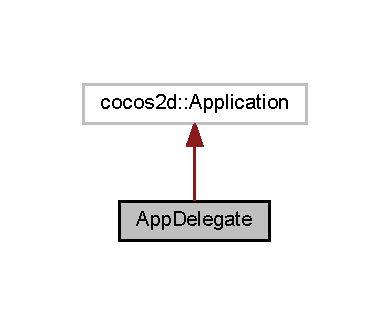
\includegraphics[width=187pt]{class_app_delegate__inherit__graph}
\end{center}
\end{figure}
\subsection*{Открытые члены}
\begin{DoxyCompactItemize}
\item 
\mbox{\Hypertarget{class_app_delegate_a7d26ade6fbc9d35ecc9185792303f82d}\label{class_app_delegate_a7d26ade6fbc9d35ecc9185792303f82d}} 
\hyperlink{class_app_delegate_a7d26ade6fbc9d35ecc9185792303f82d}{App\+Delegate} ()
\begin{DoxyCompactList}\small\item\em Конструктор по умолчанию \end{DoxyCompactList}\item 
\mbox{\Hypertarget{class_app_delegate_a9f89424b5e296e3668deaa0265fc5ac1}\label{class_app_delegate_a9f89424b5e296e3668deaa0265fc5ac1}} 
virtual \hyperlink{class_app_delegate_a9f89424b5e296e3668deaa0265fc5ac1}{$\sim$\+App\+Delegate} ()
\begin{DoxyCompactList}\small\item\em Деструктор \end{DoxyCompactList}\item 
\mbox{\Hypertarget{class_app_delegate_a2de4e8ab7d04bde311684e1d4ceb2c0f}\label{class_app_delegate_a2de4e8ab7d04bde311684e1d4ceb2c0f}} 
virtual void \hyperlink{class_app_delegate_a2de4e8ab7d04bde311684e1d4ceb2c0f}{init\+G\+L\+Context\+Attrs} ()
\begin{DoxyCompactList}\small\item\em Функция для установки атрибутов Open\+GL (красный, зеленый, синий, альфа-\/канал...) \end{DoxyCompactList}\item 
virtual bool \hyperlink{class_app_delegate_a68cbaed49edf7581dc59a09d5062fff3}{application\+Did\+Finish\+Launching} ()
\item 
\mbox{\Hypertarget{class_app_delegate_a17cb09777419781698324e0415bffd3a}\label{class_app_delegate_a17cb09777419781698324e0415bffd3a}} 
virtual void \hyperlink{class_app_delegate_a17cb09777419781698324e0415bffd3a}{application\+Did\+Enter\+Background} ()
\begin{DoxyCompactList}\small\item\em Функция вызывается, когда приложение скрывается \end{DoxyCompactList}\item 
\mbox{\Hypertarget{class_app_delegate_ac4d653e3f74a91efef5f2def58fe3108}\label{class_app_delegate_ac4d653e3f74a91efef5f2def58fe3108}} 
virtual void \hyperlink{class_app_delegate_ac4d653e3f74a91efef5f2def58fe3108}{application\+Will\+Enter\+Foreground} ()
\begin{DoxyCompactList}\small\item\em Функция вызывается при первом запуске приложения \end{DoxyCompactList}\end{DoxyCompactItemize}


\subsection{Подробное описание}
Приложение, основанное на Cocos2d. 

\subsection{Методы}
\mbox{\Hypertarget{class_app_delegate_a68cbaed49edf7581dc59a09d5062fff3}\label{class_app_delegate_a68cbaed49edf7581dc59a09d5062fff3}} 
\index{App\+Delegate@{App\+Delegate}!application\+Did\+Finish\+Launching@{application\+Did\+Finish\+Launching}}
\index{application\+Did\+Finish\+Launching@{application\+Did\+Finish\+Launching}!App\+Delegate@{App\+Delegate}}
\subsubsection{\texorpdfstring{application\+Did\+Finish\+Launching()}{applicationDidFinishLaunching()}}
{\footnotesize\ttfamily bool App\+Delegate\+::application\+Did\+Finish\+Launching (\begin{DoxyParamCaption}{ }\end{DoxyParamCaption})\hspace{0.3cm}{\ttfamily [virtual]}}

Функция для инициализации Director\textquotesingle{}а и Scene\textquotesingle{}ы \begin{DoxyReturn}{Возвращает}
true Инициализация успешна, приложение продолжает выполняться 

false Инициализация провалилась, приложение закроется 
\end{DoxyReturn}


Объявления и описания членов классов находятся в файлах\+:\begin{DoxyCompactItemize}
\item 
C\+:/\+Users/\+Vladimir/\+Documents/\+Visual Studio 2017/\+Projects/\+R\+T\+M/\+Classes/App\+Delegate.\+h\item 
C\+:/\+Users/\+Vladimir/\+Documents/\+Visual Studio 2017/\+Projects/\+R\+T\+M/\+Classes/App\+Delegate.\+cpp\end{DoxyCompactItemize}

\hypertarget{classrtm_1_1_building_object}{}\section{Класс rtm\+:\+:Building\+Object}
\label{classrtm_1_1_building_object}\index{rtm\+::\+Building\+Object@{rtm\+::\+Building\+Object}}


Класс, описывающий строения (здания)  




{\ttfamily \#include $<$Building\+Object.\+h$>$}



Граф наследования\+:rtm\+:\+:Building\+Object\+:
\nopagebreak
\begin{figure}[H]
\begin{center}
\leavevmode
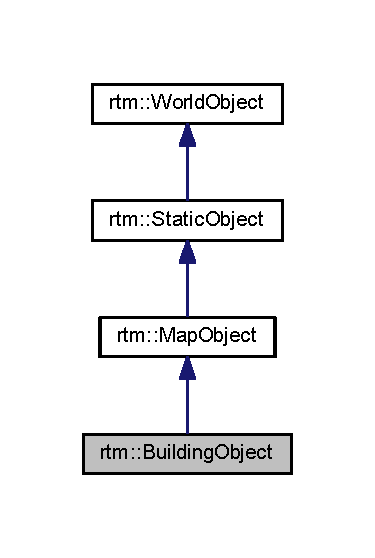
\includegraphics[width=180pt]{classrtm_1_1_building_object__inherit__graph}
\end{center}
\end{figure}
\subsection*{Открытые члены}
\begin{DoxyCompactItemize}
\item 
\mbox{\Hypertarget{classrtm_1_1_building_object_a03e7024f6e30929fd991bd811d6a7766}\label{classrtm_1_1_building_object_a03e7024f6e30929fd991bd811d6a7766}} 
\hyperlink{classrtm_1_1_building_object_a03e7024f6e30929fd991bd811d6a7766}{Building\+Object} ()
\begin{DoxyCompactList}\small\item\em Конструктор по умочанию \end{DoxyCompactList}\item 
\hyperlink{classrtm_1_1_building_object_a972c352ad972bec2381137299a95045c}{Building\+Object} (cocos2d\+::\+Sprite $\ast$const sprite, int column, int row, float angle)
\item 
\hyperlink{classrtm_1_1_building_object_a8507652023a31117c99593625011a456}{Building\+Object} (std\+::string const \&filename, int column, int row, float angle)
\item 
\hyperlink{classrtm_1_1_building_object_a3785e78d68f62e698013091d436e943d}{Building\+Object} (size\+\_\+t type, int column, int row, float angle)
\item 
\mbox{\Hypertarget{classrtm_1_1_building_object_a6c339422b4b701fb1e3208ad4a9f737a}\label{classrtm_1_1_building_object_a6c339422b4b701fb1e3208ad4a9f737a}} 
virtual \hyperlink{classrtm_1_1_building_object_a6c339422b4b701fb1e3208ad4a9f737a}{$\sim$\+Building\+Object} ()=default
\begin{DoxyCompactList}\small\item\em Деструктор по умолчанию \end{DoxyCompactList}\end{DoxyCompactItemize}
\subsection*{Дополнительные унаследованные члены}


\subsection{Подробное описание}
Класс, описывающий строения (здания) 

\subsection{Конструктор(ы)}
\mbox{\Hypertarget{classrtm_1_1_building_object_a972c352ad972bec2381137299a95045c}\label{classrtm_1_1_building_object_a972c352ad972bec2381137299a95045c}} 
\index{rtm\+::\+Building\+Object@{rtm\+::\+Building\+Object}!Building\+Object@{Building\+Object}}
\index{Building\+Object@{Building\+Object}!rtm\+::\+Building\+Object@{rtm\+::\+Building\+Object}}
\subsubsection{\texorpdfstring{Building\+Object()}{BuildingObject()}\hspace{0.1cm}{\footnotesize\ttfamily [1/3]}}
{\footnotesize\ttfamily rtm\+::\+Building\+Object\+::\+Building\+Object (\begin{DoxyParamCaption}\item[{cocos2d\+::\+Sprite $\ast$const}]{sprite,  }\item[{int}]{column,  }\item[{int}]{row,  }\item[{float}]{angle }\end{DoxyParamCaption})}

Конструктор с использованием уже готового спрайта 
\begin{DoxyParams}{Аргументы}
{\em sprite} & указатель на готовый спрайт \\
\hline
{\em column} & колонка, в которой необходимо отрисовать строение \\
\hline
{\em row} & строка, в которой необходимо отрисовать строение \\
\hline
{\em angle} & угол поворота строения \\
\hline
\end{DoxyParams}
\mbox{\Hypertarget{classrtm_1_1_building_object_a8507652023a31117c99593625011a456}\label{classrtm_1_1_building_object_a8507652023a31117c99593625011a456}} 
\index{rtm\+::\+Building\+Object@{rtm\+::\+Building\+Object}!Building\+Object@{Building\+Object}}
\index{Building\+Object@{Building\+Object}!rtm\+::\+Building\+Object@{rtm\+::\+Building\+Object}}
\subsubsection{\texorpdfstring{Building\+Object()}{BuildingObject()}\hspace{0.1cm}{\footnotesize\ttfamily [2/3]}}
{\footnotesize\ttfamily rtm\+::\+Building\+Object\+::\+Building\+Object (\begin{DoxyParamCaption}\item[{std\+::string const \&}]{filename,  }\item[{int}]{column,  }\item[{int}]{row,  }\item[{float}]{angle }\end{DoxyParamCaption})}

Конструктор из файла 
\begin{DoxyParams}{Аргументы}
{\em filename} & путь к файлу инициализации \\
\hline
{\em column} & колонка, в которой необходимо отрисовать строение \\
\hline
{\em row} & строка, в которой необходимо отрисовать строение \\
\hline
{\em angle} & угол поворота строения \\
\hline
\end{DoxyParams}
\mbox{\Hypertarget{classrtm_1_1_building_object_a3785e78d68f62e698013091d436e943d}\label{classrtm_1_1_building_object_a3785e78d68f62e698013091d436e943d}} 
\index{rtm\+::\+Building\+Object@{rtm\+::\+Building\+Object}!Building\+Object@{Building\+Object}}
\index{Building\+Object@{Building\+Object}!rtm\+::\+Building\+Object@{rtm\+::\+Building\+Object}}
\subsubsection{\texorpdfstring{Building\+Object()}{BuildingObject()}\hspace{0.1cm}{\footnotesize\ttfamily [3/3]}}
{\footnotesize\ttfamily rtm\+::\+Building\+Object\+::\+Building\+Object (\begin{DoxyParamCaption}\item[{size\+\_\+t}]{type,  }\item[{int}]{column,  }\item[{int}]{row,  }\item[{float}]{angle }\end{DoxyParamCaption})}

Конструктор стандартного строения 
\begin{DoxyParams}{Аргументы}
{\em type} & стандартный тип строения \\
\hline
{\em column} & колонка, в которой необходимо отрисовать строение \\
\hline
{\em row} & строка, в которой необходимо отрисовать строение \\
\hline
{\em angle} & угол поворота строения \\
\hline
\end{DoxyParams}


Объявления и описания членов классов находятся в файлах\+:\begin{DoxyCompactItemize}
\item 
C\+:/\+Users/\+Vladimir/\+Documents/\+Visual Studio 2017/\+Projects/\+R\+T\+M/\+Classes/Building\+Object.\+h\item 
C\+:/\+Users/\+Vladimir/\+Documents/\+Visual Studio 2017/\+Projects/\+R\+T\+M/\+Classes/Building\+Object.\+cpp\end{DoxyCompactItemize}

\hypertarget{classrtm_1_1_car_object}{}\section{Класс rtm\+:\+:Car\+Object}
\label{classrtm_1_1_car_object}\index{rtm\+::\+Car\+Object@{rtm\+::\+Car\+Object}}


Класс, описывающий машины  




{\ttfamily \#include $<$Car\+Object.\+h$>$}



Граф наследования\+:rtm\+:\+:Car\+Object\+:
\nopagebreak
\begin{figure}[H]
\begin{center}
\leavevmode
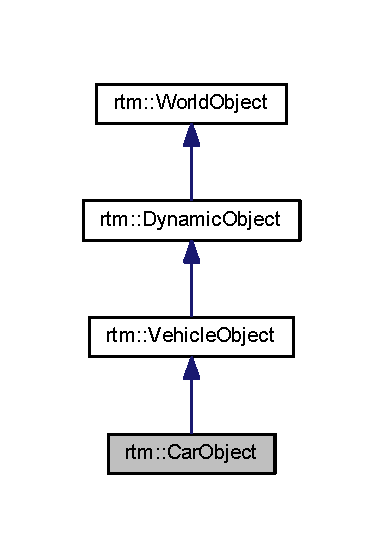
\includegraphics[width=184pt]{classrtm_1_1_car_object__inherit__graph}
\end{center}
\end{figure}
\subsection*{Открытые члены}
\begin{DoxyCompactItemize}
\item 
\mbox{\Hypertarget{classrtm_1_1_car_object_a7cc3a1d53d77c6b68e9b915455d41532}\label{classrtm_1_1_car_object_a7cc3a1d53d77c6b68e9b915455d41532}} 
\hyperlink{classrtm_1_1_car_object_a7cc3a1d53d77c6b68e9b915455d41532}{Car\+Object} ()
\begin{DoxyCompactList}\small\item\em Конструктор по умочанию \end{DoxyCompactList}\item 
\hyperlink{classrtm_1_1_car_object_af260c7e577da1e4dd75d11ae73deb1e2}{Car\+Object} (cocos2d\+::\+Sprite $\ast$const sprite, int column, int row, float angle, float max\+Speed, float acceleration)
\item 
\hyperlink{classrtm_1_1_car_object_a1f376fdc4f75df46cefc98051b05be4b}{Car\+Object} (std\+::string const \&filename, int column, int row, float angle, float max\+Speed, float acceleration)
\item 
\hyperlink{classrtm_1_1_car_object_a9f40742f9e1deb7746c9207205be73b4}{Car\+Object} (size\+\_\+t type, int column, int row, float angle)
\item 
\mbox{\Hypertarget{classrtm_1_1_car_object_a6af110bb8064a0b32ffe97a72e3645cf}\label{classrtm_1_1_car_object_a6af110bb8064a0b32ffe97a72e3645cf}} 
virtual \hyperlink{classrtm_1_1_car_object_a6af110bb8064a0b32ffe97a72e3645cf}{$\sim$\+Car\+Object} ()=default
\begin{DoxyCompactList}\small\item\em Деструктор по умолчанию \end{DoxyCompactList}\end{DoxyCompactItemize}
\subsection*{Защищенные члены}
\begin{DoxyCompactItemize}
\item 
virtual bool \hyperlink{classrtm_1_1_car_object_abbedfee1e8db8b12ea912d77efc4805c}{Movement\+Start\+\_\+} (\hyperlink{classrtm_1_1_world_controller}{World\+Controller} $\ast$const world) override
\item 
virtual bool \hyperlink{classrtm_1_1_car_object_abe89fea4893e244d9f6fb17c596b5ae0}{Movement\+Tick\+\_\+} (\hyperlink{classrtm_1_1_world_controller}{World\+Controller} $\ast$const world) override
\item 
virtual bool \hyperlink{classrtm_1_1_car_object_a24354013f953386699bbb3f4464adb0c}{Movement\+End\+\_\+} (\hyperlink{classrtm_1_1_world_controller}{World\+Controller} $\ast$const world) override
\item 
virtual bool \hyperlink{classrtm_1_1_car_object_a34063664a03d36d1308c80e064d1ae61}{Line\+Changing\+Start} (\hyperlink{classrtm_1_1_world_controller}{World\+Controller} $\ast$const world) override
\end{DoxyCompactItemize}
\subsection*{Закрытые члены}
\begin{DoxyCompactItemize}
\item 
\mbox{\Hypertarget{classrtm_1_1_car_object_a7b2f6f775bca42de1f8a171967ef4a5b}\label{classrtm_1_1_car_object_a7b2f6f775bca42de1f8a171967ef4a5b}} 
void \hyperlink{classrtm_1_1_car_object_a7b2f6f775bca42de1f8a171967ef4a5b}{Set\+Desired\+Speed\+\_\+} (float speed)
\begin{DoxyCompactList}\small\item\em Функция для установки желаемой скорости \end{DoxyCompactList}\item 
\mbox{\Hypertarget{classrtm_1_1_car_object_ac7d862334533fc10e079cec616f1c143}\label{classrtm_1_1_car_object_ac7d862334533fc10e079cec616f1c143}} 
void \hyperlink{classrtm_1_1_car_object_ac7d862334533fc10e079cec616f1c143}{Reset\+Desired\+Speed\+\_\+} ()
\begin{DoxyCompactList}\small\item\em Функция для сброса желаемой скорости \end{DoxyCompactList}\item 
void \hyperlink{classrtm_1_1_car_object_a9e80c9029d84c425b43d6a0559d0c76c}{Check\+Coating\+Ahead\+\_\+} (\hyperlink{classrtm_1_1_world_controller}{World\+Controller} $\ast$const world)
\item 
void \hyperlink{classrtm_1_1_car_object_a0cd1f15e3b28edde4271b92da250339f}{Check\+Coating\+Union\+Ahead\+\_\+} (\hyperlink{classrtm_1_1_world_controller}{World\+Controller} $\ast$const world)
\item 
void \hyperlink{classrtm_1_1_car_object_a8d8a11c484ce1afd532b78688345f314}{Check\+Road\+Ahead\+\_\+} (\hyperlink{classrtm_1_1_world_controller}{World\+Controller} $\ast$const world)
\end{DoxyCompactItemize}
\subsection*{Закрытые статические члены}
\begin{DoxyCompactItemize}
\item 
static float \hyperlink{classrtm_1_1_car_object_a0e69f04edd9f51f57a1d0fd39e2b0976}{Get\+Class\+Max\+Speed\+\_\+} (size\+\_\+t id)
\item 
static float \hyperlink{classrtm_1_1_car_object_a45d798bf2079173c677358b4b54d4e2b}{Get\+Class\+Acceleration\+\_\+} (size\+\_\+t id)
\end{DoxyCompactItemize}
\subsection*{Закрытые данные}
\begin{DoxyCompactItemize}
\item 
\mbox{\Hypertarget{classrtm_1_1_car_object_aeacdd9e29292eb69f5af3cef31aa02f7}\label{classrtm_1_1_car_object_aeacdd9e29292eb69f5af3cef31aa02f7}} 
float \hyperlink{classrtm_1_1_car_object_aeacdd9e29292eb69f5af3cef31aa02f7}{recommended\+Speed\+\_\+}
\begin{DoxyCompactList}\small\item\em Рекомендованная скорость \end{DoxyCompactList}\item 
\mbox{\Hypertarget{classrtm_1_1_car_object_a1f90afc8d2b0787b7db6b183cb58159d}\label{classrtm_1_1_car_object_a1f90afc8d2b0787b7db6b183cb58159d}} 
float \hyperlink{classrtm_1_1_car_object_a1f90afc8d2b0787b7db6b183cb58159d}{desired\+Speed\+\_\+}
\begin{DoxyCompactList}\small\item\em Желаемая скорость (приоритетнее рекомендуемой) \end{DoxyCompactList}\item 
\mbox{\Hypertarget{classrtm_1_1_car_object_a4b41298c7c17d671a0676cafebf76543}\label{classrtm_1_1_car_object_a4b41298c7c17d671a0676cafebf76543}} 
bool \hyperlink{classrtm_1_1_car_object_a4b41298c7c17d671a0676cafebf76543}{has\+Desired\+Speed\+\_\+}
\begin{DoxyCompactList}\small\item\em Задана ли желаемая скорость \end{DoxyCompactList}\item 
\mbox{\Hypertarget{classrtm_1_1_car_object_afedeeee4a90fe5febf5e164537cd9e3c}\label{classrtm_1_1_car_object_afedeeee4a90fe5febf5e164537cd9e3c}} 
bool \hyperlink{classrtm_1_1_car_object_afedeeee4a90fe5febf5e164537cd9e3c}{is\+Turn\+Near\+\_\+}
\begin{DoxyCompactList}\small\item\em Далеко ли следующий поворот \end{DoxyCompactList}\item 
\mbox{\Hypertarget{classrtm_1_1_car_object_ae8dd4d2009bfee2951559f3207e26e1a}\label{classrtm_1_1_car_object_ae8dd4d2009bfee2951559f3207e26e1a}} 
bool \hyperlink{classrtm_1_1_car_object_ae8dd4d2009bfee2951559f3207e26e1a}{is\+Right\+Turn\+\_\+}
\begin{DoxyCompactList}\small\item\em Напрвление следующего поворота \end{DoxyCompactList}\item 
\mbox{\Hypertarget{classrtm_1_1_car_object_a041532281ad637e2bf604f43089d6425}\label{classrtm_1_1_car_object_a041532281ad637e2bf604f43089d6425}} 
bool \hyperlink{classrtm_1_1_car_object_a041532281ad637e2bf604f43089d6425}{wait\+For\+Signal\+\_\+}
\begin{DoxyCompactList}\small\item\em Происходит ли сейчас ожидание сигнала светофора \end{DoxyCompactList}\item 
\mbox{\Hypertarget{classrtm_1_1_car_object_ac9d8672c56c5b0aef99e05553a6b0acd}\label{classrtm_1_1_car_object_ac9d8672c56c5b0aef99e05553a6b0acd}} 
bool \hyperlink{classrtm_1_1_car_object_ac9d8672c56c5b0aef99e05553a6b0acd}{wait\+For\+Turn\+\_\+}
\begin{DoxyCompactList}\small\item\em Происходит ли сейчас ожидание освобождения нерегулируемого перекрестка \end{DoxyCompactList}\item 
\mbox{\Hypertarget{classrtm_1_1_car_object_ae1ca1a36a1ebd0cb49759a3ff16f5885}\label{classrtm_1_1_car_object_ae1ca1a36a1ebd0cb49759a3ff16f5885}} 
\hyperlink{namespacertm_a69dc82b16a0148c10962caa83d930f89}{Angle\+Type} \hyperlink{classrtm_1_1_car_object_ae1ca1a36a1ebd0cb49759a3ff16f5885}{desired\+Direction\+\_\+}
\begin{DoxyCompactList}\small\item\em Желаемое направление движения (при первой возможности машина повернет) \end{DoxyCompactList}\end{DoxyCompactItemize}


\subsection{Подробное описание}
Класс, описывающий машины 

\subsection{Конструктор(ы)}
\mbox{\Hypertarget{classrtm_1_1_car_object_af260c7e577da1e4dd75d11ae73deb1e2}\label{classrtm_1_1_car_object_af260c7e577da1e4dd75d11ae73deb1e2}} 
\index{rtm\+::\+Car\+Object@{rtm\+::\+Car\+Object}!Car\+Object@{Car\+Object}}
\index{Car\+Object@{Car\+Object}!rtm\+::\+Car\+Object@{rtm\+::\+Car\+Object}}
\subsubsection{\texorpdfstring{Car\+Object()}{CarObject()}\hspace{0.1cm}{\footnotesize\ttfamily [1/3]}}
{\footnotesize\ttfamily rtm\+::\+Car\+Object\+::\+Car\+Object (\begin{DoxyParamCaption}\item[{cocos2d\+::\+Sprite $\ast$const}]{sprite,  }\item[{int}]{column,  }\item[{int}]{row,  }\item[{float}]{angle,  }\item[{float}]{max\+Speed,  }\item[{float}]{acceleration }\end{DoxyParamCaption})}

Конструктор с использованием уже готового спрайта 
\begin{DoxyParams}{Аргументы}
{\em sprite} & указатель на готовый спрайт \\
\hline
{\em column} & колонка, в которой необходимо отрисовать машину \\
\hline
{\em row} & строка, в которой необходимо отрисовать машину \\
\hline
{\em angle} & угол поворота машины \\
\hline
{\em max\+Speed} & максимальная скорость машины \\
\hline
{\em acceleration} & ускорение машины \\
\hline
\end{DoxyParams}
\mbox{\Hypertarget{classrtm_1_1_car_object_a1f376fdc4f75df46cefc98051b05be4b}\label{classrtm_1_1_car_object_a1f376fdc4f75df46cefc98051b05be4b}} 
\index{rtm\+::\+Car\+Object@{rtm\+::\+Car\+Object}!Car\+Object@{Car\+Object}}
\index{Car\+Object@{Car\+Object}!rtm\+::\+Car\+Object@{rtm\+::\+Car\+Object}}
\subsubsection{\texorpdfstring{Car\+Object()}{CarObject()}\hspace{0.1cm}{\footnotesize\ttfamily [2/3]}}
{\footnotesize\ttfamily rtm\+::\+Car\+Object\+::\+Car\+Object (\begin{DoxyParamCaption}\item[{std\+::string const \&}]{filename,  }\item[{int}]{column,  }\item[{int}]{row,  }\item[{float}]{angle,  }\item[{float}]{max\+Speed,  }\item[{float}]{acceleration }\end{DoxyParamCaption})}

Конструктор из файла 
\begin{DoxyParams}{Аргументы}
{\em filename} & путь к файлу инициализации \\
\hline
{\em column} & колонка, в которой необходимо отрисовать машину \\
\hline
{\em row} & строка, в которой необходимо отрисовать машину \\
\hline
{\em angle} & угол поворота машины \\
\hline
{\em max\+Speed} & максимальная скорость машины \\
\hline
{\em acceleration} & ускорение машины \\
\hline
\end{DoxyParams}
\mbox{\Hypertarget{classrtm_1_1_car_object_a9f40742f9e1deb7746c9207205be73b4}\label{classrtm_1_1_car_object_a9f40742f9e1deb7746c9207205be73b4}} 
\index{rtm\+::\+Car\+Object@{rtm\+::\+Car\+Object}!Car\+Object@{Car\+Object}}
\index{Car\+Object@{Car\+Object}!rtm\+::\+Car\+Object@{rtm\+::\+Car\+Object}}
\subsubsection{\texorpdfstring{Car\+Object()}{CarObject()}\hspace{0.1cm}{\footnotesize\ttfamily [3/3]}}
{\footnotesize\ttfamily rtm\+::\+Car\+Object\+::\+Car\+Object (\begin{DoxyParamCaption}\item[{size\+\_\+t}]{type,  }\item[{int}]{column,  }\item[{int}]{row,  }\item[{float}]{angle }\end{DoxyParamCaption})}

Конструктор стандартной машины 
\begin{DoxyParams}{Аргументы}
{\em type} & стандартный тип машины \\
\hline
{\em column} & колонка, в которой необходимо отрисовать машину \\
\hline
{\em row} & строка, в которой необходимо отрисовать машину \\
\hline
{\em angle} & угол поворота машины \\
\hline
\end{DoxyParams}


\subsection{Методы}
\mbox{\Hypertarget{classrtm_1_1_car_object_abbedfee1e8db8b12ea912d77efc4805c}\label{classrtm_1_1_car_object_abbedfee1e8db8b12ea912d77efc4805c}} 
\index{rtm\+::\+Car\+Object@{rtm\+::\+Car\+Object}!Movement\+Start\+\_\+@{Movement\+Start\+\_\+}}
\index{Movement\+Start\+\_\+@{Movement\+Start\+\_\+}!rtm\+::\+Car\+Object@{rtm\+::\+Car\+Object}}
\subsubsection{\texorpdfstring{Movement\+Start\+\_\+()}{MovementStart\_()}}
{\footnotesize\ttfamily bool rtm\+::\+Car\+Object\+::\+Movement\+Start\+\_\+ (\begin{DoxyParamCaption}\item[{\hyperlink{classrtm_1_1_world_controller}{World\+Controller} $\ast$const}]{world }\end{DoxyParamCaption})\hspace{0.3cm}{\ttfamily [override]}, {\ttfamily [protected]}, {\ttfamily [virtual]}}

Функция, которая просто пропускает выполнение родителя 
\begin{DoxyParams}{Аргументы}
{\em world} & контроллер мира, в котором находится объект \\
\hline
\end{DoxyParams}


Переопределяет метод предка \hyperlink{classrtm_1_1_vehicle_object_aa02e0b8f3fa159939f370938e45abf88}{rtm\+::\+Vehicle\+Object}.

\mbox{\Hypertarget{classrtm_1_1_car_object_abe89fea4893e244d9f6fb17c596b5ae0}\label{classrtm_1_1_car_object_abe89fea4893e244d9f6fb17c596b5ae0}} 
\index{rtm\+::\+Car\+Object@{rtm\+::\+Car\+Object}!Movement\+Tick\+\_\+@{Movement\+Tick\+\_\+}}
\index{Movement\+Tick\+\_\+@{Movement\+Tick\+\_\+}!rtm\+::\+Car\+Object@{rtm\+::\+Car\+Object}}
\subsubsection{\texorpdfstring{Movement\+Tick\+\_\+()}{MovementTick\_()}}
{\footnotesize\ttfamily bool rtm\+::\+Car\+Object\+::\+Movement\+Tick\+\_\+ (\begin{DoxyParamCaption}\item[{\hyperlink{classrtm_1_1_world_controller}{World\+Controller} $\ast$const}]{world }\end{DoxyParamCaption})\hspace{0.3cm}{\ttfamily [override]}, {\ttfamily [protected]}, {\ttfamily [virtual]}}

Функция для вычисления скорости 
\begin{DoxyParams}{Аргументы}
{\em world} & контроллер мира, в котором находится объект \\
\hline
\end{DoxyParams}


Переопределяет метод предка \hyperlink{classrtm_1_1_vehicle_object_a06a920b3fe0df4fa4ca0687a9366426a}{rtm\+::\+Vehicle\+Object}.

\mbox{\Hypertarget{classrtm_1_1_car_object_a24354013f953386699bbb3f4464adb0c}\label{classrtm_1_1_car_object_a24354013f953386699bbb3f4464adb0c}} 
\index{rtm\+::\+Car\+Object@{rtm\+::\+Car\+Object}!Movement\+End\+\_\+@{Movement\+End\+\_\+}}
\index{Movement\+End\+\_\+@{Movement\+End\+\_\+}!rtm\+::\+Car\+Object@{rtm\+::\+Car\+Object}}
\subsubsection{\texorpdfstring{Movement\+End\+\_\+()}{MovementEnd\_()}}
{\footnotesize\ttfamily bool rtm\+::\+Car\+Object\+::\+Movement\+End\+\_\+ (\begin{DoxyParamCaption}\item[{\hyperlink{classrtm_1_1_world_controller}{World\+Controller} $\ast$const}]{world }\end{DoxyParamCaption})\hspace{0.3cm}{\ttfamily [override]}, {\ttfamily [protected]}, {\ttfamily [virtual]}}

Функция обнуляет финальную скорость 
\begin{DoxyParams}{Аргументы}
{\em world} & контроллер мира, в котором находится объект \\
\hline
\end{DoxyParams}


Переопределяет метод предка \hyperlink{classrtm_1_1_vehicle_object_a7e6c94902d1d544006ca8de63ba36860}{rtm\+::\+Vehicle\+Object}.

\mbox{\Hypertarget{classrtm_1_1_car_object_a34063664a03d36d1308c80e064d1ae61}\label{classrtm_1_1_car_object_a34063664a03d36d1308c80e064d1ae61}} 
\index{rtm\+::\+Car\+Object@{rtm\+::\+Car\+Object}!Line\+Changing\+Start@{Line\+Changing\+Start}}
\index{Line\+Changing\+Start@{Line\+Changing\+Start}!rtm\+::\+Car\+Object@{rtm\+::\+Car\+Object}}
\subsubsection{\texorpdfstring{Line\+Changing\+Start()}{LineChangingStart()}}
{\footnotesize\ttfamily bool rtm\+::\+Car\+Object\+::\+Line\+Changing\+Start (\begin{DoxyParamCaption}\item[{\hyperlink{classrtm_1_1_world_controller}{World\+Controller} $\ast$const}]{world }\end{DoxyParamCaption})\hspace{0.3cm}{\ttfamily [override]}, {\ttfamily [protected]}, {\ttfamily [virtual]}}

Функция, описывающая движение перед перестроением 
\begin{DoxyParams}{Аргументы}
{\em world} & контроллер мира, в котором находится объект \\
\hline
\end{DoxyParams}


Переопределяет метод предка \hyperlink{classrtm_1_1_vehicle_object_a8976be533dfa4704f7b221c79d1fce99}{rtm\+::\+Vehicle\+Object}.

\mbox{\Hypertarget{classrtm_1_1_car_object_a9e80c9029d84c425b43d6a0559d0c76c}\label{classrtm_1_1_car_object_a9e80c9029d84c425b43d6a0559d0c76c}} 
\index{rtm\+::\+Car\+Object@{rtm\+::\+Car\+Object}!Check\+Coating\+Ahead\+\_\+@{Check\+Coating\+Ahead\+\_\+}}
\index{Check\+Coating\+Ahead\+\_\+@{Check\+Coating\+Ahead\+\_\+}!rtm\+::\+Car\+Object@{rtm\+::\+Car\+Object}}
\subsubsection{\texorpdfstring{Check\+Coating\+Ahead\+\_\+()}{CheckCoatingAhead\_()}}
{\footnotesize\ttfamily void rtm\+::\+Car\+Object\+::\+Check\+Coating\+Ahead\+\_\+ (\begin{DoxyParamCaption}\item[{\hyperlink{classrtm_1_1_world_controller}{World\+Controller} $\ast$const}]{world }\end{DoxyParamCaption})\hspace{0.3cm}{\ttfamily [private]}}

Функция для проверки объекта (повороты и т.\+д.) 
\begin{DoxyParams}{Аргументы}
{\em world} & контроллер мира, в котором находится объект \\
\hline
\end{DoxyParams}
\mbox{\Hypertarget{classrtm_1_1_car_object_a0cd1f15e3b28edde4271b92da250339f}\label{classrtm_1_1_car_object_a0cd1f15e3b28edde4271b92da250339f}} 
\index{rtm\+::\+Car\+Object@{rtm\+::\+Car\+Object}!Check\+Coating\+Union\+Ahead\+\_\+@{Check\+Coating\+Union\+Ahead\+\_\+}}
\index{Check\+Coating\+Union\+Ahead\+\_\+@{Check\+Coating\+Union\+Ahead\+\_\+}!rtm\+::\+Car\+Object@{rtm\+::\+Car\+Object}}
\subsubsection{\texorpdfstring{Check\+Coating\+Union\+Ahead\+\_\+()}{CheckCoatingUnionAhead\_()}}
{\footnotesize\ttfamily void rtm\+::\+Car\+Object\+::\+Check\+Coating\+Union\+Ahead\+\_\+ (\begin{DoxyParamCaption}\item[{\hyperlink{classrtm_1_1_world_controller}{World\+Controller} $\ast$const}]{world }\end{DoxyParamCaption})\hspace{0.3cm}{\ttfamily [private]}}

Функция для проверки объединения покрытий (заранее тормозим перед светофорами и т.\+д.) 
\begin{DoxyParams}{Аргументы}
{\em world} & контроллер мира, в котором находится объект \\
\hline
\end{DoxyParams}
\mbox{\Hypertarget{classrtm_1_1_car_object_a8d8a11c484ce1afd532b78688345f314}\label{classrtm_1_1_car_object_a8d8a11c484ce1afd532b78688345f314}} 
\index{rtm\+::\+Car\+Object@{rtm\+::\+Car\+Object}!Check\+Road\+Ahead\+\_\+@{Check\+Road\+Ahead\+\_\+}}
\index{Check\+Road\+Ahead\+\_\+@{Check\+Road\+Ahead\+\_\+}!rtm\+::\+Car\+Object@{rtm\+::\+Car\+Object}}
\subsubsection{\texorpdfstring{Check\+Road\+Ahead\+\_\+()}{CheckRoadAhead\_()}}
{\footnotesize\ttfamily void rtm\+::\+Car\+Object\+::\+Check\+Road\+Ahead\+\_\+ (\begin{DoxyParamCaption}\item[{\hyperlink{classrtm_1_1_world_controller}{World\+Controller} $\ast$const}]{world }\end{DoxyParamCaption})\hspace{0.3cm}{\ttfamily [private]}}

Функция для проверки дороги спереди (принятие решений) 
\begin{DoxyParams}{Аргументы}
{\em world} & контроллер мира, в котором находится объект \\
\hline
\end{DoxyParams}
\mbox{\Hypertarget{classrtm_1_1_car_object_a0e69f04edd9f51f57a1d0fd39e2b0976}\label{classrtm_1_1_car_object_a0e69f04edd9f51f57a1d0fd39e2b0976}} 
\index{rtm\+::\+Car\+Object@{rtm\+::\+Car\+Object}!Get\+Class\+Max\+Speed\+\_\+@{Get\+Class\+Max\+Speed\+\_\+}}
\index{Get\+Class\+Max\+Speed\+\_\+@{Get\+Class\+Max\+Speed\+\_\+}!rtm\+::\+Car\+Object@{rtm\+::\+Car\+Object}}
\subsubsection{\texorpdfstring{Get\+Class\+Max\+Speed\+\_\+()}{GetClassMaxSpeed\_()}}
{\footnotesize\ttfamily float rtm\+::\+Car\+Object\+::\+Get\+Class\+Max\+Speed\+\_\+ (\begin{DoxyParamCaption}\item[{size\+\_\+t}]{id }\end{DoxyParamCaption})\hspace{0.3cm}{\ttfamily [static]}, {\ttfamily [private]}}

Функция для получения максимальной скорости стандартной машины по номеру 
\begin{DoxyParams}{Аргументы}
{\em id} & номер стандартной машины \\
\hline
\end{DoxyParams}
\begin{DoxyReturn}{Возвращает}
максимальная скорость машины 
\end{DoxyReturn}
\mbox{\Hypertarget{classrtm_1_1_car_object_a45d798bf2079173c677358b4b54d4e2b}\label{classrtm_1_1_car_object_a45d798bf2079173c677358b4b54d4e2b}} 
\index{rtm\+::\+Car\+Object@{rtm\+::\+Car\+Object}!Get\+Class\+Acceleration\+\_\+@{Get\+Class\+Acceleration\+\_\+}}
\index{Get\+Class\+Acceleration\+\_\+@{Get\+Class\+Acceleration\+\_\+}!rtm\+::\+Car\+Object@{rtm\+::\+Car\+Object}}
\subsubsection{\texorpdfstring{Get\+Class\+Acceleration\+\_\+()}{GetClassAcceleration\_()}}
{\footnotesize\ttfamily float rtm\+::\+Car\+Object\+::\+Get\+Class\+Acceleration\+\_\+ (\begin{DoxyParamCaption}\item[{size\+\_\+t}]{id }\end{DoxyParamCaption})\hspace{0.3cm}{\ttfamily [static]}, {\ttfamily [private]}}

Функция для получения ускорения стандартной машины по номеру 
\begin{DoxyParams}{Аргументы}
{\em id} & номер стандартной машины \\
\hline
\end{DoxyParams}
\begin{DoxyReturn}{Возвращает}
ускорение машины 
\end{DoxyReturn}


Объявления и описания членов классов находятся в файлах\+:\begin{DoxyCompactItemize}
\item 
C\+:/\+Users/\+Vladimir/\+Documents/\+Visual Studio 2017/\+Projects/\+R\+T\+M/\+Classes/Car\+Object.\+h\item 
C\+:/\+Users/\+Vladimir/\+Documents/\+Visual Studio 2017/\+Projects/\+R\+T\+M/\+Classes/Car\+Object.\+cpp\end{DoxyCompactItemize}

\hypertarget{classrtm_1_1_coating_object}{}\section{Класс rtm\+:\+:Coating\+Object}
\label{classrtm_1_1_coating_object}\index{rtm\+::\+Coating\+Object@{rtm\+::\+Coating\+Object}}


Класс покрытия секции карты  




{\ttfamily \#include $<$Coating\+Object.\+h$>$}



Граф наследования\+:rtm\+:\+:Coating\+Object\+:
\nopagebreak
\begin{figure}[H]
\begin{center}
\leavevmode
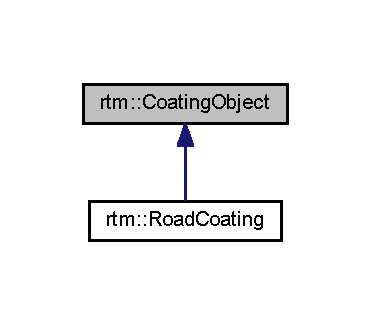
\includegraphics[width=290pt]{classrtm_1_1_coating_object__inherit__graph}
\end{center}
\end{figure}
\subsection*{Открытые члены}
\begin{DoxyCompactItemize}
\item 
\mbox{\Hypertarget{classrtm_1_1_coating_object_a4b6f326b459b1bbf6b66c08cd74d2f1a}\label{classrtm_1_1_coating_object_a4b6f326b459b1bbf6b66c08cd74d2f1a}} 
\hyperlink{classrtm_1_1_coating_object_a4b6f326b459b1bbf6b66c08cd74d2f1a}{Coating\+Object} ()
\begin{DoxyCompactList}\small\item\em Конструктор по умолчанию \end{DoxyCompactList}\item 
\hyperlink{classrtm_1_1_coating_object_a4d5d7ecc1ba34ec9f2d29dd39c1c054f}{Coating\+Object} (cocos2d\+::\+Sprite $\ast$const sprite, int column, int row, \hyperlink{namespacertm_a69dc82b16a0148c10962caa83d930f89}{Angle\+Type} angle, float resistance, \hyperlink{namespacertm_a4776fbfe59834ff1a16838ad6735b69a}{Directions} directions)
\item 
\hyperlink{classrtm_1_1_coating_object_ae3cfac6ecad1d4e35a34f80aaf782392}{Coating\+Object} (std\+::string const \&filename, int column, int row, \hyperlink{namespacertm_a69dc82b16a0148c10962caa83d930f89}{Angle\+Type} angle, float resistance, \hyperlink{namespacertm_a4776fbfe59834ff1a16838ad6735b69a}{Directions} directions)
\item 
\mbox{\Hypertarget{classrtm_1_1_coating_object_aa181401eddb2b9c099c0d56dcbae4d0d}\label{classrtm_1_1_coating_object_aa181401eddb2b9c099c0d56dcbae4d0d}} 
virtual \hyperlink{classrtm_1_1_coating_object_aa181401eddb2b9c099c0d56dcbae4d0d}{$\sim$\+Coating\+Object} ()=default
\begin{DoxyCompactList}\small\item\em Деструктор по умолчанию \end{DoxyCompactList}\item 
cocos2d\+::\+Sprite $\ast$ \hyperlink{classrtm_1_1_coating_object_a5153c2be68353078dac8771cc9c361bb}{Get\+Sprite} () const
\item 
float \hyperlink{classrtm_1_1_coating_object_a1680b004da834a1b885b4e22f09e84cc}{Get\+Resistance} () const
\item 
bool \hyperlink{classrtm_1_1_coating_object_a88eb5287d899ca8e10e31de4192bbddc}{Has\+Direction} (\hyperlink{namespacertm_a69dc82b16a0148c10962caa83d930f89}{Angle\+Type} angle) const
\item 
bool \hyperlink{classrtm_1_1_coating_object_a4d7656260eaa296f1bfa2e957698c437}{Is\+Direction\+Available} (\hyperlink{namespacertm_a69dc82b16a0148c10962caa83d930f89}{Angle\+Type} angle) const
\item 
void \hyperlink{classrtm_1_1_coating_object_a93eb37a24af3939337f6330209fae809}{Set\+Direction\+Availability} (\hyperlink{namespacertm_a69dc82b16a0148c10962caa83d930f89}{Angle\+Type} angle, bool status)
\end{DoxyCompactItemize}
\subsection*{Защищенные члены}
\begin{DoxyCompactItemize}
\item 
void \hyperlink{classrtm_1_1_coating_object_a1d0227cd023ce6e6bd475194b5cbfe2d}{Set\+Sprite\+\_\+} (cocos2d\+::\+Sprite $\ast$const sprite)
\end{DoxyCompactItemize}
\subsection*{Закрытые члены}
\begin{DoxyCompactItemize}
\item 
void \hyperlink{classrtm_1_1_coating_object_a5bb5e11400d05dc2d50bfbd2021d3aac}{Set\+X\+\_\+} (float x)
\item 
void \hyperlink{classrtm_1_1_coating_object_a3f67f750f8bf4b87a55655018c0c8d71}{Set\+Y\+\_\+} (float y)
\end{DoxyCompactItemize}
\subsection*{Закрытые данные}
\begin{DoxyCompactItemize}
\item 
\mbox{\Hypertarget{classrtm_1_1_coating_object_a5a50d8dce6f4c8f62869eac82b362b4b}\label{classrtm_1_1_coating_object_a5a50d8dce6f4c8f62869eac82b362b4b}} 
cocos2d\+::\+Sprite $\ast$ \hyperlink{classrtm_1_1_coating_object_a5a50d8dce6f4c8f62869eac82b362b4b}{sprite\+\_\+}
\begin{DoxyCompactList}\small\item\em Указатель на спрайт \end{DoxyCompactList}\item 
\mbox{\Hypertarget{classrtm_1_1_coating_object_af0952d3d8f3a52dc6f7da2b12a8728bc}\label{classrtm_1_1_coating_object_af0952d3d8f3a52dc6f7da2b12a8728bc}} 
float \hyperlink{classrtm_1_1_coating_object_af0952d3d8f3a52dc6f7da2b12a8728bc}{x\+\_\+}
\begin{DoxyCompactList}\small\item\em Абсцисса \end{DoxyCompactList}\item 
\mbox{\Hypertarget{classrtm_1_1_coating_object_a9aa381d87a817ab61a55f94538d9b6e0}\label{classrtm_1_1_coating_object_a9aa381d87a817ab61a55f94538d9b6e0}} 
float \hyperlink{classrtm_1_1_coating_object_a9aa381d87a817ab61a55f94538d9b6e0}{y\+\_\+}
\begin{DoxyCompactList}\small\item\em Ордината \end{DoxyCompactList}\item 
\mbox{\Hypertarget{classrtm_1_1_coating_object_a254720b1a903d8a0359f5d3ebe774bfb}\label{classrtm_1_1_coating_object_a254720b1a903d8a0359f5d3ebe774bfb}} 
float \hyperlink{classrtm_1_1_coating_object_a254720b1a903d8a0359f5d3ebe774bfb}{resistance\+\_\+}
\begin{DoxyCompactList}\small\item\em Сопротивление на покрытии \end{DoxyCompactList}\item 
\mbox{\Hypertarget{classrtm_1_1_coating_object_a41be26c25937bd71ecbb5e1527446841}\label{classrtm_1_1_coating_object_a41be26c25937bd71ecbb5e1527446841}} 
\hyperlink{namespacertm_a4776fbfe59834ff1a16838ad6735b69a}{Directions} \hyperlink{classrtm_1_1_coating_object_a41be26c25937bd71ecbb5e1527446841}{directions\+\_\+}
\begin{DoxyCompactList}\small\item\em Доступные направления \end{DoxyCompactList}\item 
\mbox{\Hypertarget{classrtm_1_1_coating_object_ad542a00f5a714fee4f8ebc30e76746cc}\label{classrtm_1_1_coating_object_ad542a00f5a714fee4f8ebc30e76746cc}} 
\hyperlink{namespacertm_a4776fbfe59834ff1a16838ad6735b69a}{Directions} \hyperlink{classrtm_1_1_coating_object_ad542a00f5a714fee4f8ebc30e76746cc}{available\+Directions\+\_\+}
\begin{DoxyCompactList}\small\item\em Разрешенные направления \end{DoxyCompactList}\end{DoxyCompactItemize}


\subsection{Подробное описание}
Класс покрытия секции карты 

\subsection{Конструктор(ы)}
\mbox{\Hypertarget{classrtm_1_1_coating_object_a4d5d7ecc1ba34ec9f2d29dd39c1c054f}\label{classrtm_1_1_coating_object_a4d5d7ecc1ba34ec9f2d29dd39c1c054f}} 
\index{rtm\+::\+Coating\+Object@{rtm\+::\+Coating\+Object}!Coating\+Object@{Coating\+Object}}
\index{Coating\+Object@{Coating\+Object}!rtm\+::\+Coating\+Object@{rtm\+::\+Coating\+Object}}
\subsubsection{\texorpdfstring{Coating\+Object()}{CoatingObject()}\hspace{0.1cm}{\footnotesize\ttfamily [1/2]}}
{\footnotesize\ttfamily rtm\+::\+Coating\+Object\+::\+Coating\+Object (\begin{DoxyParamCaption}\item[{cocos2d\+::\+Sprite $\ast$const}]{sprite,  }\item[{int}]{column,  }\item[{int}]{row,  }\item[{\hyperlink{namespacertm_a69dc82b16a0148c10962caa83d930f89}{Angle\+Type}}]{angle,  }\item[{float}]{resistance,  }\item[{\hyperlink{namespacertm_a4776fbfe59834ff1a16838ad6735b69a}{Directions}}]{directions }\end{DoxyParamCaption})}

Конструктор с использованием уже готового спрайта 
\begin{DoxyParams}{Аргументы}
{\em sprite} & указатель на готовый спрайт \\
\hline
{\em column} & колонка, в которой необходимо отрисовать объект \\
\hline
{\em row} & строка, в которой необходимо отрисовать объект \\
\hline
{\em angle} & угол поворота объекта \\
\hline
{\em resistance} & коэффициент сопротивления на покрытии \\
\hline
{\em directions} & доступные направления для движения \\
\hline
\end{DoxyParams}
\mbox{\Hypertarget{classrtm_1_1_coating_object_ae3cfac6ecad1d4e35a34f80aaf782392}\label{classrtm_1_1_coating_object_ae3cfac6ecad1d4e35a34f80aaf782392}} 
\index{rtm\+::\+Coating\+Object@{rtm\+::\+Coating\+Object}!Coating\+Object@{Coating\+Object}}
\index{Coating\+Object@{Coating\+Object}!rtm\+::\+Coating\+Object@{rtm\+::\+Coating\+Object}}
\subsubsection{\texorpdfstring{Coating\+Object()}{CoatingObject()}\hspace{0.1cm}{\footnotesize\ttfamily [2/2]}}
{\footnotesize\ttfamily rtm\+::\+Coating\+Object\+::\+Coating\+Object (\begin{DoxyParamCaption}\item[{std\+::string const \&}]{filename,  }\item[{int}]{column,  }\item[{int}]{row,  }\item[{\hyperlink{namespacertm_a69dc82b16a0148c10962caa83d930f89}{Angle\+Type}}]{angle,  }\item[{float}]{resistance,  }\item[{\hyperlink{namespacertm_a4776fbfe59834ff1a16838ad6735b69a}{Directions}}]{directions }\end{DoxyParamCaption})}

Конструктор из файла 
\begin{DoxyParams}{Аргументы}
{\em filename} & путь к файлу инициализации \\
\hline
{\em column} & колонка, в которой необходимо отрисовать объект \\
\hline
{\em row} & строка, в которой необходимо отрисовать объект \\
\hline
{\em angle} & угол поворота объекта \\
\hline
{\em resistance} & коэффициент сопротивления на покрытии \\
\hline
{\em directions} & доступные направления для движения \\
\hline
\end{DoxyParams}


\subsection{Методы}
\mbox{\Hypertarget{classrtm_1_1_coating_object_a5153c2be68353078dac8771cc9c361bb}\label{classrtm_1_1_coating_object_a5153c2be68353078dac8771cc9c361bb}} 
\index{rtm\+::\+Coating\+Object@{rtm\+::\+Coating\+Object}!Get\+Sprite@{Get\+Sprite}}
\index{Get\+Sprite@{Get\+Sprite}!rtm\+::\+Coating\+Object@{rtm\+::\+Coating\+Object}}
\subsubsection{\texorpdfstring{Get\+Sprite()}{GetSprite()}}
{\footnotesize\ttfamily cocos2d\+::\+Sprite $\ast$ rtm\+::\+Coating\+Object\+::\+Get\+Sprite (\begin{DoxyParamCaption}{ }\end{DoxyParamCaption}) const}

Функция для получения спрайта \begin{DoxyReturn}{Возвращает}
указатель на спрайт 
\end{DoxyReturn}
\mbox{\Hypertarget{classrtm_1_1_coating_object_a1680b004da834a1b885b4e22f09e84cc}\label{classrtm_1_1_coating_object_a1680b004da834a1b885b4e22f09e84cc}} 
\index{rtm\+::\+Coating\+Object@{rtm\+::\+Coating\+Object}!Get\+Resistance@{Get\+Resistance}}
\index{Get\+Resistance@{Get\+Resistance}!rtm\+::\+Coating\+Object@{rtm\+::\+Coating\+Object}}
\subsubsection{\texorpdfstring{Get\+Resistance()}{GetResistance()}}
{\footnotesize\ttfamily float rtm\+::\+Coating\+Object\+::\+Get\+Resistance (\begin{DoxyParamCaption}{ }\end{DoxyParamCaption}) const}

Функция для получения коэффициента сопротивления на покрытии \begin{DoxyReturn}{Возвращает}
сопротивление 
\end{DoxyReturn}
\mbox{\Hypertarget{classrtm_1_1_coating_object_a88eb5287d899ca8e10e31de4192bbddc}\label{classrtm_1_1_coating_object_a88eb5287d899ca8e10e31de4192bbddc}} 
\index{rtm\+::\+Coating\+Object@{rtm\+::\+Coating\+Object}!Has\+Direction@{Has\+Direction}}
\index{Has\+Direction@{Has\+Direction}!rtm\+::\+Coating\+Object@{rtm\+::\+Coating\+Object}}
\subsubsection{\texorpdfstring{Has\+Direction()}{HasDirection()}}
{\footnotesize\ttfamily bool rtm\+::\+Coating\+Object\+::\+Has\+Direction (\begin{DoxyParamCaption}\item[{\hyperlink{namespacertm_a69dc82b16a0148c10962caa83d930f89}{Angle\+Type}}]{angle }\end{DoxyParamCaption}) const}

Функция для проверки существования направления 
\begin{DoxyParams}{Аргументы}
{\em angle} & направление \\
\hline
\end{DoxyParams}
\begin{DoxyReturn}{Возвращает}
true, если доступно (существует), иначе false 
\end{DoxyReturn}
\mbox{\Hypertarget{classrtm_1_1_coating_object_a4d7656260eaa296f1bfa2e957698c437}\label{classrtm_1_1_coating_object_a4d7656260eaa296f1bfa2e957698c437}} 
\index{rtm\+::\+Coating\+Object@{rtm\+::\+Coating\+Object}!Is\+Direction\+Available@{Is\+Direction\+Available}}
\index{Is\+Direction\+Available@{Is\+Direction\+Available}!rtm\+::\+Coating\+Object@{rtm\+::\+Coating\+Object}}
\subsubsection{\texorpdfstring{Is\+Direction\+Available()}{IsDirectionAvailable()}}
{\footnotesize\ttfamily bool rtm\+::\+Coating\+Object\+::\+Is\+Direction\+Available (\begin{DoxyParamCaption}\item[{\hyperlink{namespacertm_a69dc82b16a0148c10962caa83d930f89}{Angle\+Type}}]{angle }\end{DoxyParamCaption}) const}

Функция для проверки разрешенности направления 
\begin{DoxyParams}{Аргументы}
{\em angle} & направление \\
\hline
\end{DoxyParams}
\begin{DoxyReturn}{Возвращает}
true, если разрешено ехать в данном направлении, иначе false 
\end{DoxyReturn}
\mbox{\Hypertarget{classrtm_1_1_coating_object_a93eb37a24af3939337f6330209fae809}\label{classrtm_1_1_coating_object_a93eb37a24af3939337f6330209fae809}} 
\index{rtm\+::\+Coating\+Object@{rtm\+::\+Coating\+Object}!Set\+Direction\+Availability@{Set\+Direction\+Availability}}
\index{Set\+Direction\+Availability@{Set\+Direction\+Availability}!rtm\+::\+Coating\+Object@{rtm\+::\+Coating\+Object}}
\subsubsection{\texorpdfstring{Set\+Direction\+Availability()}{SetDirectionAvailability()}}
{\footnotesize\ttfamily void rtm\+::\+Coating\+Object\+::\+Set\+Direction\+Availability (\begin{DoxyParamCaption}\item[{\hyperlink{namespacertm_a69dc82b16a0148c10962caa83d930f89}{Angle\+Type}}]{angle,  }\item[{bool}]{status }\end{DoxyParamCaption})}

Функция установки разрешенности направления 
\begin{DoxyParams}{Аргументы}
{\em angle} & направление \\
\hline
{\em status} & разрешено ли ехать \\
\hline
\end{DoxyParams}
\mbox{\Hypertarget{classrtm_1_1_coating_object_a1d0227cd023ce6e6bd475194b5cbfe2d}\label{classrtm_1_1_coating_object_a1d0227cd023ce6e6bd475194b5cbfe2d}} 
\index{rtm\+::\+Coating\+Object@{rtm\+::\+Coating\+Object}!Set\+Sprite\+\_\+@{Set\+Sprite\+\_\+}}
\index{Set\+Sprite\+\_\+@{Set\+Sprite\+\_\+}!rtm\+::\+Coating\+Object@{rtm\+::\+Coating\+Object}}
\subsubsection{\texorpdfstring{Set\+Sprite\+\_\+()}{SetSprite\_()}}
{\footnotesize\ttfamily void rtm\+::\+Coating\+Object\+::\+Set\+Sprite\+\_\+ (\begin{DoxyParamCaption}\item[{cocos2d\+::\+Sprite $\ast$const}]{sprite }\end{DoxyParamCaption})\hspace{0.3cm}{\ttfamily [protected]}}

Функция для установки спрайта 
\begin{DoxyParams}{Аргументы}
{\em sprite} & указатель на спрайт \\
\hline
\end{DoxyParams}
\mbox{\Hypertarget{classrtm_1_1_coating_object_a5bb5e11400d05dc2d50bfbd2021d3aac}\label{classrtm_1_1_coating_object_a5bb5e11400d05dc2d50bfbd2021d3aac}} 
\index{rtm\+::\+Coating\+Object@{rtm\+::\+Coating\+Object}!Set\+X\+\_\+@{Set\+X\+\_\+}}
\index{Set\+X\+\_\+@{Set\+X\+\_\+}!rtm\+::\+Coating\+Object@{rtm\+::\+Coating\+Object}}
\subsubsection{\texorpdfstring{Set\+X\+\_\+()}{SetX\_()}}
{\footnotesize\ttfamily void rtm\+::\+Coating\+Object\+::\+Set\+X\+\_\+ (\begin{DoxyParamCaption}\item[{float}]{x }\end{DoxyParamCaption})\hspace{0.3cm}{\ttfamily [private]}}

Функция для установки абсциссы 
\begin{DoxyParams}{Аргументы}
{\em x} & абсцисса \\
\hline
\end{DoxyParams}
\mbox{\Hypertarget{classrtm_1_1_coating_object_a3f67f750f8bf4b87a55655018c0c8d71}\label{classrtm_1_1_coating_object_a3f67f750f8bf4b87a55655018c0c8d71}} 
\index{rtm\+::\+Coating\+Object@{rtm\+::\+Coating\+Object}!Set\+Y\+\_\+@{Set\+Y\+\_\+}}
\index{Set\+Y\+\_\+@{Set\+Y\+\_\+}!rtm\+::\+Coating\+Object@{rtm\+::\+Coating\+Object}}
\subsubsection{\texorpdfstring{Set\+Y\+\_\+()}{SetY\_()}}
{\footnotesize\ttfamily void rtm\+::\+Coating\+Object\+::\+Set\+Y\+\_\+ (\begin{DoxyParamCaption}\item[{float}]{y }\end{DoxyParamCaption})\hspace{0.3cm}{\ttfamily [private]}}

Функция для установки ординаты 
\begin{DoxyParams}{Аргументы}
{\em y} & ордината \\
\hline
\end{DoxyParams}


Объявления и описания членов классов находятся в файлах\+:\begin{DoxyCompactItemize}
\item 
C\+:/\+Users/\+Vladimir/\+Documents/\+Visual Studio 2017/\+Projects/\+R\+T\+M/\+Classes/Coating\+Object.\+h\item 
C\+:/\+Users/\+Vladimir/\+Documents/\+Visual Studio 2017/\+Projects/\+R\+T\+M/\+Classes/Coating\+Object.\+cpp\end{DoxyCompactItemize}

\hypertarget{classrtm_1_1_coating_union}{}\section{Класс rtm\+:\+:Coating\+Union}
\label{classrtm_1_1_coating_union}\index{rtm\+::\+Coating\+Union@{rtm\+::\+Coating\+Union}}


{\ttfamily \#include $<$Coating\+Union.\+h$>$}



Граф наследования\+:rtm\+:\+:Coating\+Union\+:
\nopagebreak
\begin{figure}[H]
\begin{center}
\leavevmode
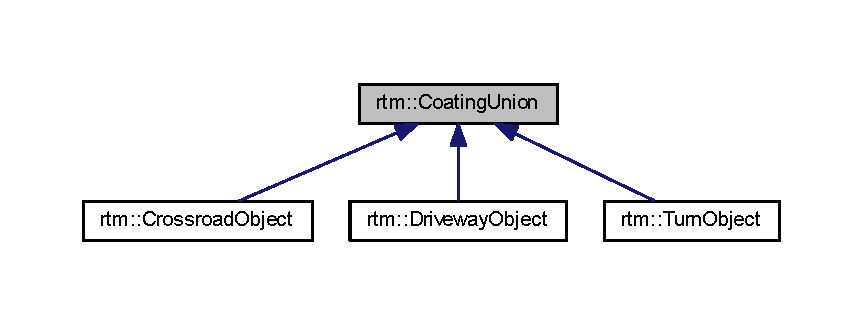
\includegraphics[width=350pt]{classrtm_1_1_coating_union__inherit__graph}
\end{center}
\end{figure}
\subsection*{Открытые члены}
\begin{DoxyCompactItemize}
\item 
\mbox{\Hypertarget{classrtm_1_1_coating_union_aada3c299db0c6604b8a713d2ae87afbb}\label{classrtm_1_1_coating_union_aada3c299db0c6604b8a713d2ae87afbb}} 
\hyperlink{classrtm_1_1_coating_union_aada3c299db0c6604b8a713d2ae87afbb}{Coating\+Union} ()
\begin{DoxyCompactList}\small\item\em Конструктор по умолчанию \end{DoxyCompactList}\item 
\hyperlink{classrtm_1_1_coating_union_ad5c97fb37269028e9058c37c10428255}{Coating\+Union} (\hyperlink{namespacertm_a6a0d424be5696f64038e5e84a79cabfa}{Coating\+Union\+Type} type, int column, int row, \hyperlink{namespacertm_ae3bb29510cfde424975be31866d2486e}{Coating\+Matrix} \&\&objects)
\item 
\mbox{\Hypertarget{classrtm_1_1_coating_union_a42d7554ae47b709c6518b84a9afe9a70}\label{classrtm_1_1_coating_union_a42d7554ae47b709c6518b84a9afe9a70}} 
virtual \hyperlink{classrtm_1_1_coating_union_a42d7554ae47b709c6518b84a9afe9a70}{$\sim$\+Coating\+Union} ()=default
\begin{DoxyCompactList}\small\item\em Деструктор по умолчанию \end{DoxyCompactList}\item 
\hyperlink{namespacertm_a6a0d424be5696f64038e5e84a79cabfa}{Coating\+Union\+Type} \hyperlink{classrtm_1_1_coating_union_a6e679033a648837c2df2b3b1ea749efd}{Get\+Type} () const
\item 
size\+\_\+t \hyperlink{classrtm_1_1_coating_union_aca7956667dce60916e9cd225694a2818}{Get\+Width} () const
\item 
size\+\_\+t \hyperlink{classrtm_1_1_coating_union_ac9530320f820757aec11c51bcf8eb3cc}{Get\+Height} () const
\item 
\hyperlink{namespacertm_ab0ec616a26920aeaf720d04e041e8ce3}{Coating\+Unique} const  \& \hyperlink{classrtm_1_1_coating_union_acbcdbbd157f6d55597a54bb639a977f2}{Get\+Coating\+Object} (int column, int row) const
\item 
virtual float \hyperlink{classrtm_1_1_coating_union_adf3ec4f4e8399c455aaa73bfe726b4ce}{Get\+Length} () const
\item 
bool \hyperlink{classrtm_1_1_coating_union_a7f77378af1ea7473d10497ad01effcad}{Is\+Correct\+Column} (int column) const
\item 
bool \hyperlink{classrtm_1_1_coating_union_abbd51ea78ee3d798807827f6ee930540}{Is\+Correct\+Row} (int row) const
\item 
virtual void \hyperlink{classrtm_1_1_coating_union_ae95be187677aec759723edb4d14b35c1}{Show\+Sprites} (cocos2d\+::\+Layer $\ast$const layer)
\item 
virtual void \hyperlink{classrtm_1_1_coating_union_a4e046aae25ce91da0408ac31a0de4e21}{Release\+Sprites} (cocos2d\+::\+Layer $\ast$const layer)
\end{DoxyCompactItemize}
\subsection*{Защищенные члены}
\begin{DoxyCompactItemize}
\item 
int \hyperlink{classrtm_1_1_coating_union_a1d2b6a339f6cafbe41d416f371cbed04}{Get\+Column\+\_\+} () const
\item 
int \hyperlink{classrtm_1_1_coating_union_ad283fd24e0c3347c569e3ea5772a9651}{Get\+Row\+\_\+} () const
\end{DoxyCompactItemize}
\subsection*{Закрытые данные}
\begin{DoxyCompactItemize}
\item 
\mbox{\Hypertarget{classrtm_1_1_coating_union_ab8fd79074da6b4915bbbaec93befc0f0}\label{classrtm_1_1_coating_union_ab8fd79074da6b4915bbbaec93befc0f0}} 
\hyperlink{namespacertm_a6a0d424be5696f64038e5e84a79cabfa}{Coating\+Union\+Type} \hyperlink{classrtm_1_1_coating_union_ab8fd79074da6b4915bbbaec93befc0f0}{type\+\_\+}
\begin{DoxyCompactList}\small\item\em Тип объединения покрытий (получившегося элемента) \end{DoxyCompactList}\item 
\mbox{\Hypertarget{classrtm_1_1_coating_union_aef5f5d3f4ac06044fe4482bf60b01e77}\label{classrtm_1_1_coating_union_aef5f5d3f4ac06044fe4482bf60b01e77}} 
int \hyperlink{classrtm_1_1_coating_union_aef5f5d3f4ac06044fe4482bf60b01e77}{column\+\_\+}
\begin{DoxyCompactList}\small\item\em Левая колонка объединения \end{DoxyCompactList}\item 
\mbox{\Hypertarget{classrtm_1_1_coating_union_aa7133c7a2059495ab4c02b1813e8abfb}\label{classrtm_1_1_coating_union_aa7133c7a2059495ab4c02b1813e8abfb}} 
int \hyperlink{classrtm_1_1_coating_union_aa7133c7a2059495ab4c02b1813e8abfb}{row\+\_\+}
\begin{DoxyCompactList}\small\item\em Нижняя строка объединения \end{DoxyCompactList}\item 
\mbox{\Hypertarget{classrtm_1_1_coating_union_acab8ed30a66c786a3ac7d0edff914dbc}\label{classrtm_1_1_coating_union_acab8ed30a66c786a3ac7d0edff914dbc}} 
size\+\_\+t \hyperlink{classrtm_1_1_coating_union_acab8ed30a66c786a3ac7d0edff914dbc}{width\+\_\+}
\begin{DoxyCompactList}\small\item\em Ширина объединения \end{DoxyCompactList}\item 
\mbox{\Hypertarget{classrtm_1_1_coating_union_abd65484b95a4b62e1c22146cb2a9d542}\label{classrtm_1_1_coating_union_abd65484b95a4b62e1c22146cb2a9d542}} 
size\+\_\+t \hyperlink{classrtm_1_1_coating_union_abd65484b95a4b62e1c22146cb2a9d542}{height\+\_\+}
\begin{DoxyCompactList}\small\item\em Высота объединения \end{DoxyCompactList}\item 
\mbox{\Hypertarget{classrtm_1_1_coating_union_a805afd44081afec9f4e286436be1a735}\label{classrtm_1_1_coating_union_a805afd44081afec9f4e286436be1a735}} 
\hyperlink{namespacertm_ae3bb29510cfde424975be31866d2486e}{Coating\+Matrix} \hyperlink{classrtm_1_1_coating_union_a805afd44081afec9f4e286436be1a735}{objects\+\_\+}
\begin{DoxyCompactList}\small\item\em @Матрица объектов покрытий \end{DoxyCompactList}\end{DoxyCompactItemize}


\subsection{Подробное описание}
Класс объединения покрытий \begin{DoxySeeAlso}{См. также}
\hyperlink{classrtm_1_1_coating_object}{Coating\+Object} 
\end{DoxySeeAlso}


\subsection{Конструктор(ы)}
\mbox{\Hypertarget{classrtm_1_1_coating_union_ad5c97fb37269028e9058c37c10428255}\label{classrtm_1_1_coating_union_ad5c97fb37269028e9058c37c10428255}} 
\index{rtm\+::\+Coating\+Union@{rtm\+::\+Coating\+Union}!Coating\+Union@{Coating\+Union}}
\index{Coating\+Union@{Coating\+Union}!rtm\+::\+Coating\+Union@{rtm\+::\+Coating\+Union}}
\subsubsection{\texorpdfstring{Coating\+Union()}{CoatingUnion()}}
{\footnotesize\ttfamily rtm\+::\+Coating\+Union\+::\+Coating\+Union (\begin{DoxyParamCaption}\item[{\hyperlink{namespacertm_a6a0d424be5696f64038e5e84a79cabfa}{Coating\+Union\+Type}}]{type,  }\item[{int}]{column,  }\item[{int}]{row,  }\item[{\hyperlink{namespacertm_ae3bb29510cfde424975be31866d2486e}{Coating\+Matrix} \&\&}]{objects }\end{DoxyParamCaption})}

Конструктор по матрице покрытий 
\begin{DoxyParams}{Аргументы}
{\em type} & тип объединения покрытий (получившегося элемента) \\
\hline
{\em column} & левая колонка объединения \\
\hline
{\em row} & нижняя строка объединения \\
\hline
{\em objects} & матрица объектов покрытий \\
\hline
\end{DoxyParams}


\subsection{Методы}
\mbox{\Hypertarget{classrtm_1_1_coating_union_a6e679033a648837c2df2b3b1ea749efd}\label{classrtm_1_1_coating_union_a6e679033a648837c2df2b3b1ea749efd}} 
\index{rtm\+::\+Coating\+Union@{rtm\+::\+Coating\+Union}!Get\+Type@{Get\+Type}}
\index{Get\+Type@{Get\+Type}!rtm\+::\+Coating\+Union@{rtm\+::\+Coating\+Union}}
\subsubsection{\texorpdfstring{Get\+Type()}{GetType()}}
{\footnotesize\ttfamily \hyperlink{namespacertm_a6a0d424be5696f64038e5e84a79cabfa}{rtm\+::\+Coating\+Union\+Type} rtm\+::\+Coating\+Union\+::\+Get\+Type (\begin{DoxyParamCaption}{ }\end{DoxyParamCaption}) const}

Функция для получения типа объединения \begin{DoxyReturn}{Возвращает}
тип объединения 
\end{DoxyReturn}
\mbox{\Hypertarget{classrtm_1_1_coating_union_aca7956667dce60916e9cd225694a2818}\label{classrtm_1_1_coating_union_aca7956667dce60916e9cd225694a2818}} 
\index{rtm\+::\+Coating\+Union@{rtm\+::\+Coating\+Union}!Get\+Width@{Get\+Width}}
\index{Get\+Width@{Get\+Width}!rtm\+::\+Coating\+Union@{rtm\+::\+Coating\+Union}}
\subsubsection{\texorpdfstring{Get\+Width()}{GetWidth()}}
{\footnotesize\ttfamily size\+\_\+t rtm\+::\+Coating\+Union\+::\+Get\+Width (\begin{DoxyParamCaption}{ }\end{DoxyParamCaption}) const}

Функция для получения ширины объединения \begin{DoxyReturn}{Возвращает}
ширина объединения 
\end{DoxyReturn}
\mbox{\Hypertarget{classrtm_1_1_coating_union_ac9530320f820757aec11c51bcf8eb3cc}\label{classrtm_1_1_coating_union_ac9530320f820757aec11c51bcf8eb3cc}} 
\index{rtm\+::\+Coating\+Union@{rtm\+::\+Coating\+Union}!Get\+Height@{Get\+Height}}
\index{Get\+Height@{Get\+Height}!rtm\+::\+Coating\+Union@{rtm\+::\+Coating\+Union}}
\subsubsection{\texorpdfstring{Get\+Height()}{GetHeight()}}
{\footnotesize\ttfamily size\+\_\+t rtm\+::\+Coating\+Union\+::\+Get\+Height (\begin{DoxyParamCaption}{ }\end{DoxyParamCaption}) const}

Функция для получения высоты объединения \begin{DoxyReturn}{Возвращает}
высота объединения 
\end{DoxyReturn}
\mbox{\Hypertarget{classrtm_1_1_coating_union_acbcdbbd157f6d55597a54bb639a977f2}\label{classrtm_1_1_coating_union_acbcdbbd157f6d55597a54bb639a977f2}} 
\index{rtm\+::\+Coating\+Union@{rtm\+::\+Coating\+Union}!Get\+Coating\+Object@{Get\+Coating\+Object}}
\index{Get\+Coating\+Object@{Get\+Coating\+Object}!rtm\+::\+Coating\+Union@{rtm\+::\+Coating\+Union}}
\subsubsection{\texorpdfstring{Get\+Coating\+Object()}{GetCoatingObject()}}
{\footnotesize\ttfamily \hyperlink{namespacertm_ab0ec616a26920aeaf720d04e041e8ce3}{rtm\+::\+Coating\+Unique} const  \& rtm\+::\+Coating\+Union\+::\+Get\+Coating\+Object (\begin{DoxyParamCaption}\item[{int}]{column,  }\item[{int}]{row }\end{DoxyParamCaption}) const}

Функция для получения объекта 
\begin{DoxyParams}{Аргументы}
{\em column} & колонка (относительно всей карты), в которой находится объект \\
\hline
{\em row} & строка (относительно всей карты), в которой находится объект \\
\hline
\end{DoxyParams}
\begin{DoxyReturn}{Возвращает}
умный указатель на объект 
\end{DoxyReturn}
\mbox{\Hypertarget{classrtm_1_1_coating_union_adf3ec4f4e8399c455aaa73bfe726b4ce}\label{classrtm_1_1_coating_union_adf3ec4f4e8399c455aaa73bfe726b4ce}} 
\index{rtm\+::\+Coating\+Union@{rtm\+::\+Coating\+Union}!Get\+Length@{Get\+Length}}
\index{Get\+Length@{Get\+Length}!rtm\+::\+Coating\+Union@{rtm\+::\+Coating\+Union}}
\subsubsection{\texorpdfstring{Get\+Length()}{GetLength()}}
{\footnotesize\ttfamily float rtm\+::\+Coating\+Union\+::\+Get\+Length (\begin{DoxyParamCaption}{ }\end{DoxyParamCaption}) const\hspace{0.3cm}{\ttfamily [virtual]}}

Функция для получения длины (количества покрытий) \begin{DoxyReturn}{Возвращает}
длина 
\end{DoxyReturn}


Переопределяется в \hyperlink{classrtm_1_1_driveway_object_a5de41ef395ad8ccefb435e568f84ed40}{rtm\+::\+Driveway\+Object}.

\mbox{\Hypertarget{classrtm_1_1_coating_union_a7f77378af1ea7473d10497ad01effcad}\label{classrtm_1_1_coating_union_a7f77378af1ea7473d10497ad01effcad}} 
\index{rtm\+::\+Coating\+Union@{rtm\+::\+Coating\+Union}!Is\+Correct\+Column@{Is\+Correct\+Column}}
\index{Is\+Correct\+Column@{Is\+Correct\+Column}!rtm\+::\+Coating\+Union@{rtm\+::\+Coating\+Union}}
\subsubsection{\texorpdfstring{Is\+Correct\+Column()}{IsCorrectColumn()}}
{\footnotesize\ttfamily bool rtm\+::\+Coating\+Union\+::\+Is\+Correct\+Column (\begin{DoxyParamCaption}\item[{int}]{column }\end{DoxyParamCaption}) const}

Функция для проверки корректности колонки в данном объединении \begin{DoxyReturn}{Возвращает}
true, если объединение содержит данную колонку, иначе false 
\end{DoxyReturn}
\mbox{\Hypertarget{classrtm_1_1_coating_union_abbd51ea78ee3d798807827f6ee930540}\label{classrtm_1_1_coating_union_abbd51ea78ee3d798807827f6ee930540}} 
\index{rtm\+::\+Coating\+Union@{rtm\+::\+Coating\+Union}!Is\+Correct\+Row@{Is\+Correct\+Row}}
\index{Is\+Correct\+Row@{Is\+Correct\+Row}!rtm\+::\+Coating\+Union@{rtm\+::\+Coating\+Union}}
\subsubsection{\texorpdfstring{Is\+Correct\+Row()}{IsCorrectRow()}}
{\footnotesize\ttfamily bool rtm\+::\+Coating\+Union\+::\+Is\+Correct\+Row (\begin{DoxyParamCaption}\item[{int}]{row }\end{DoxyParamCaption}) const}

Функция для проверки корректности строки в данном объединении \begin{DoxyReturn}{Возвращает}
true, если объединение содержит данную строку, иначе false 
\end{DoxyReturn}
\mbox{\Hypertarget{classrtm_1_1_coating_union_ae95be187677aec759723edb4d14b35c1}\label{classrtm_1_1_coating_union_ae95be187677aec759723edb4d14b35c1}} 
\index{rtm\+::\+Coating\+Union@{rtm\+::\+Coating\+Union}!Show\+Sprites@{Show\+Sprites}}
\index{Show\+Sprites@{Show\+Sprites}!rtm\+::\+Coating\+Union@{rtm\+::\+Coating\+Union}}
\subsubsection{\texorpdfstring{Show\+Sprites()}{ShowSprites()}}
{\footnotesize\ttfamily void rtm\+::\+Coating\+Union\+::\+Show\+Sprites (\begin{DoxyParamCaption}\item[{cocos2d\+::\+Layer $\ast$const}]{layer }\end{DoxyParamCaption})\hspace{0.3cm}{\ttfamily [virtual]}}

Функция для добавления спрайтов на сцену 
\begin{DoxyParams}{Аргументы}
{\em layer} & слой, на который надо добавить спрайты управляющего блока \\
\hline
\end{DoxyParams}


Переопределяется в \hyperlink{classrtm_1_1_crossroad_object_a2de2a5dac2ba2ca573cfa65a2633de9b}{rtm\+::\+Crossroad\+Object}.

\mbox{\Hypertarget{classrtm_1_1_coating_union_a4e046aae25ce91da0408ac31a0de4e21}\label{classrtm_1_1_coating_union_a4e046aae25ce91da0408ac31a0de4e21}} 
\index{rtm\+::\+Coating\+Union@{rtm\+::\+Coating\+Union}!Release\+Sprites@{Release\+Sprites}}
\index{Release\+Sprites@{Release\+Sprites}!rtm\+::\+Coating\+Union@{rtm\+::\+Coating\+Union}}
\subsubsection{\texorpdfstring{Release\+Sprites()}{ReleaseSprites()}}
{\footnotesize\ttfamily void rtm\+::\+Coating\+Union\+::\+Release\+Sprites (\begin{DoxyParamCaption}\item[{cocos2d\+::\+Layer $\ast$const}]{layer }\end{DoxyParamCaption})\hspace{0.3cm}{\ttfamily [virtual]}}

Функция для удаления спрайтов со сцены 
\begin{DoxyParams}{Аргументы}
{\em layer} & слой, с которого надо удалить спрайты управляющего блока \\
\hline
\end{DoxyParams}


Переопределяется в \hyperlink{classrtm_1_1_crossroad_object_a92e9357697edecc69564fd4d40524a3b}{rtm\+::\+Crossroad\+Object}.

\mbox{\Hypertarget{classrtm_1_1_coating_union_a1d2b6a339f6cafbe41d416f371cbed04}\label{classrtm_1_1_coating_union_a1d2b6a339f6cafbe41d416f371cbed04}} 
\index{rtm\+::\+Coating\+Union@{rtm\+::\+Coating\+Union}!Get\+Column\+\_\+@{Get\+Column\+\_\+}}
\index{Get\+Column\+\_\+@{Get\+Column\+\_\+}!rtm\+::\+Coating\+Union@{rtm\+::\+Coating\+Union}}
\subsubsection{\texorpdfstring{Get\+Column\+\_\+()}{GetColumn\_()}}
{\footnotesize\ttfamily int rtm\+::\+Coating\+Union\+::\+Get\+Column\+\_\+ (\begin{DoxyParamCaption}{ }\end{DoxyParamCaption}) const\hspace{0.3cm}{\ttfamily [protected]}}

Функция для получения левой колонки объединения \begin{DoxyReturn}{Возвращает}
левая колонка объединения 
\end{DoxyReturn}
\mbox{\Hypertarget{classrtm_1_1_coating_union_ad283fd24e0c3347c569e3ea5772a9651}\label{classrtm_1_1_coating_union_ad283fd24e0c3347c569e3ea5772a9651}} 
\index{rtm\+::\+Coating\+Union@{rtm\+::\+Coating\+Union}!Get\+Row\+\_\+@{Get\+Row\+\_\+}}
\index{Get\+Row\+\_\+@{Get\+Row\+\_\+}!rtm\+::\+Coating\+Union@{rtm\+::\+Coating\+Union}}
\subsubsection{\texorpdfstring{Get\+Row\+\_\+()}{GetRow\_()}}
{\footnotesize\ttfamily int rtm\+::\+Coating\+Union\+::\+Get\+Row\+\_\+ (\begin{DoxyParamCaption}{ }\end{DoxyParamCaption}) const\hspace{0.3cm}{\ttfamily [protected]}}

Функция для получения нижней строки объединения \begin{DoxyReturn}{Возвращает}
нижняя строка объединения 
\end{DoxyReturn}


Объявления и описания членов классов находятся в файлах\+:\begin{DoxyCompactItemize}
\item 
C\+:/\+Users/\+Vladimir/\+Documents/\+Visual Studio 2017/\+Projects/\+R\+T\+M/\+Classes/Coating\+Union.\+h\item 
C\+:/\+Users/\+Vladimir/\+Documents/\+Visual Studio 2017/\+Projects/\+R\+T\+M/\+Classes/Coating\+Union.\+cpp\end{DoxyCompactItemize}

\hypertarget{classrtm_1_1_control_unit}{}\section{Класс rtm\+:\+:Control\+Unit}
\label{classrtm_1_1_control_unit}\index{rtm\+::\+Control\+Unit@{rtm\+::\+Control\+Unit}}


Класс управляющего блока (светофор)  




{\ttfamily \#include $<$Control\+Unit.\+h$>$}

\subsection*{Открытые члены}
\begin{DoxyCompactItemize}
\item 
\mbox{\Hypertarget{classrtm_1_1_control_unit_a6faae9a6512a9f75fbe4c1c4b2f88090}\label{classrtm_1_1_control_unit_a6faae9a6512a9f75fbe4c1c4b2f88090}} 
\hyperlink{classrtm_1_1_control_unit_a6faae9a6512a9f75fbe4c1c4b2f88090}{Control\+Unit} ()
\begin{DoxyCompactList}\small\item\em Конструктор по умолчанию \end{DoxyCompactList}\item 
\hyperlink{classrtm_1_1_control_unit_ac8a261d763f6d6632ce2c872710fe6b4}{Control\+Unit} (size\+\_\+t type, int column, int row, \hyperlink{namespacertm_a14457f3088a92b86a96686b72d3e4eea}{Lines\+Counts} lines\+Counts)
\item 
\hyperlink{classrtm_1_1_control_unit_a2c2c1f0f0196f0af82009f94bb875736}{Control\+Unit} (size\+\_\+t type, int column, int row, \hyperlink{namespacertm_a14457f3088a92b86a96686b72d3e4eea}{Lines\+Counts} lines\+Counts, \hyperlink{namespacertm_a69dc82b16a0148c10962caa83d930f89}{Angle\+Type} null\+Direction)
\item 
\mbox{\Hypertarget{classrtm_1_1_control_unit_a29e6e147ae6212c9bc7cc13c5d8fdc2c}\label{classrtm_1_1_control_unit_a29e6e147ae6212c9bc7cc13c5d8fdc2c}} 
virtual \hyperlink{classrtm_1_1_control_unit_a29e6e147ae6212c9bc7cc13c5d8fdc2c}{$\sim$\+Control\+Unit} ()=default
\begin{DoxyCompactList}\small\item\em Деструктор по умолчанию \end{DoxyCompactList}\item 
void \hyperlink{classrtm_1_1_control_unit_afb3eba6577d912109784ac1d32338859}{Update} (\hyperlink{classrtm_1_1_world_controller}{World\+Controller} $\ast$const world)
\item 
\hyperlink{classrtm_1_1_control_unit_ab48f3a045d62fa1f251af2ece4b52d44}{operator bool} () const
\item 
\hyperlink{namespacertm_aadb7300c15d57429546fb0b7f8ee0ee6}{Signal\+Type} \hyperlink{classrtm_1_1_control_unit_afa3dcc399f2f5b7d0c1451aa65977da6}{Get\+Signal} (\hyperlink{namespacertm_a57b216f3aeb45041f3461bab08bc3aeb}{Direction\+Type} from, \hyperlink{namespacertm_a57b216f3aeb45041f3461bab08bc3aeb}{Direction\+Type} to) const
\item 
void \hyperlink{classrtm_1_1_control_unit_af126b136af6883970ded2a592c90d2b1}{Show\+Sprites} (cocos2d\+::\+Layer $\ast$const layer)
\item 
void \hyperlink{classrtm_1_1_control_unit_ac21d7c91d9c62fb58f29b2412ce4d4be}{Release\+Sprites} (cocos2d\+::\+Layer $\ast$const layer)
\end{DoxyCompactItemize}
\subsection*{Закрытые члены}
\begin{DoxyCompactItemize}
\item 
\mbox{\Hypertarget{classrtm_1_1_control_unit_aeec72cf989ee126e9fb7a7b27c486f6b}\label{classrtm_1_1_control_unit_aeec72cf989ee126e9fb7a7b27c486f6b}} 
void \hyperlink{classrtm_1_1_control_unit_aeec72cf989ee126e9fb7a7b27c486f6b}{Init\+Signals\+\_\+} ()
\begin{DoxyCompactList}\small\item\em Функция для инициализации сигналов \end{DoxyCompactList}\item 
\mbox{\Hypertarget{classrtm_1_1_control_unit_aca3d0de2c18e1b9fa1ca449e86328599}\label{classrtm_1_1_control_unit_aca3d0de2c18e1b9fa1ca449e86328599}} 
void \hyperlink{classrtm_1_1_control_unit_aca3d0de2c18e1b9fa1ca449e86328599}{Reset\+Sprites\+\_\+} ()
\begin{DoxyCompactList}\small\item\em Функция для отображения спрайтов в зависимости от массива сигналов \end{DoxyCompactList}\item 
void \hyperlink{classrtm_1_1_control_unit_afacb521a6f7297b932a48edbbf0a10b2}{Update\+Signal\+\_\+} (size\+\_\+t i, size\+\_\+t j, \hyperlink{namespacertm_aadb7300c15d57429546fb0b7f8ee0ee6}{Signal\+Type} signal)
\item 
\mbox{\Hypertarget{classrtm_1_1_control_unit_a63302a181e4f6cf8ecfc9acd24acfdb9}\label{classrtm_1_1_control_unit_a63302a181e4f6cf8ecfc9acd24acfdb9}} 
void \hyperlink{classrtm_1_1_control_unit_a63302a181e4f6cf8ecfc9acd24acfdb9}{Inc\+State\+\_\+} ()
\begin{DoxyCompactList}\small\item\em Функция для инкремента номера состояния \end{DoxyCompactList}\item 
void \hyperlink{classrtm_1_1_control_unit_adc15ad500c2e7edbe9bdac16a16a0eff}{Set\+State\+\_\+} (size\+\_\+t state)
\item 
\mbox{\Hypertarget{classrtm_1_1_control_unit_a8beeca4f58525c029a5879534304367e}\label{classrtm_1_1_control_unit_a8beeca4f58525c029a5879534304367e}} 
void \hyperlink{classrtm_1_1_control_unit_a8beeca4f58525c029a5879534304367e}{Reset\+State\+\_\+} ()
\begin{DoxyCompactList}\small\item\em Функция для сброса номера состояния \end{DoxyCompactList}\end{DoxyCompactItemize}
\subsection*{Закрытые данные}
\begin{DoxyCompactItemize}
\item 
\mbox{\Hypertarget{classrtm_1_1_control_unit_a831ba648d8df6aca6c2530bab19eae65}\label{classrtm_1_1_control_unit_a831ba648d8df6aca6c2530bab19eae65}} 
size\+\_\+t \hyperlink{classrtm_1_1_control_unit_a831ba648d8df6aca6c2530bab19eae65}{type\+\_\+}
\begin{DoxyCompactList}\small\item\em Номер типа управляющего блока (задает логику) \end{DoxyCompactList}\item 
\mbox{\Hypertarget{classrtm_1_1_control_unit_a9b3fa03f97a3f29e758e265c8ded4957}\label{classrtm_1_1_control_unit_a9b3fa03f97a3f29e758e265c8ded4957}} 
int \hyperlink{classrtm_1_1_control_unit_a9b3fa03f97a3f29e758e265c8ded4957}{column\+\_\+}
\begin{DoxyCompactList}\small\item\em Левая колонка перекрестка \end{DoxyCompactList}\item 
\mbox{\Hypertarget{classrtm_1_1_control_unit_aa3b238e5b91281a493bfb3fb24d01d66}\label{classrtm_1_1_control_unit_aa3b238e5b91281a493bfb3fb24d01d66}} 
int \hyperlink{classrtm_1_1_control_unit_aa3b238e5b91281a493bfb3fb24d01d66}{row\+\_\+}
\begin{DoxyCompactList}\small\item\em Нижняя строка перекрестка \end{DoxyCompactList}\item 
\mbox{\Hypertarget{classrtm_1_1_control_unit_a98e098f07ff00685089fa55f0b569802}\label{classrtm_1_1_control_unit_a98e098f07ff00685089fa55f0b569802}} 
\hyperlink{namespacertm_a14457f3088a92b86a96686b72d3e4eea}{Lines\+Counts} \hyperlink{classrtm_1_1_control_unit_a98e098f07ff00685089fa55f0b569802}{lines\+Counts\+\_\+}
\begin{DoxyCompactList}\small\item\em Количество полос в каждом направлении \end{DoxyCompactList}\item 
\mbox{\Hypertarget{classrtm_1_1_control_unit_a2fe9307cb649d9c6a7f122e0363bca24}\label{classrtm_1_1_control_unit_a2fe9307cb649d9c6a7f122e0363bca24}} 
\hyperlink{namespacertm_a69dc82b16a0148c10962caa83d930f89}{Angle\+Type} \hyperlink{classrtm_1_1_control_unit_a2fe9307cb649d9c6a7f122e0363bca24}{null\+Direction\+\_\+}
\begin{DoxyCompactList}\small\item\em Сторона, в направлении которой нельзя двигаться \end{DoxyCompactList}\item 
\mbox{\Hypertarget{classrtm_1_1_control_unit_aace48a89b42ac67686c879c5ae61023d}\label{classrtm_1_1_control_unit_aace48a89b42ac67686c879c5ae61023d}} 
\hyperlink{namespacertm_afa6df86cef8e2ebcc053ad994e440354}{Crossroad\+Signals} \hyperlink{classrtm_1_1_control_unit_aace48a89b42ac67686c879c5ae61023d}{signals\+\_\+}
\begin{DoxyCompactList}\small\item\em Все сигналы управляющего блока \end{DoxyCompactList}\item 
\mbox{\Hypertarget{classrtm_1_1_control_unit_a907c89505cfec93598b95c7b3e7c4664}\label{classrtm_1_1_control_unit_a907c89505cfec93598b95c7b3e7c4664}} 
\hyperlink{namespacertm_ac9f276c8ed33ee992eb1a1f04a8254a0}{Directions\+Signal\+Sprites} \hyperlink{classrtm_1_1_control_unit_a907c89505cfec93598b95c7b3e7c4664}{sprites\+\_\+}
\begin{DoxyCompactList}\small\item\em Все спрайты управляющего блока \end{DoxyCompactList}\item 
\mbox{\Hypertarget{classrtm_1_1_control_unit_a1496bfa46e8d33577118271087235e4d}\label{classrtm_1_1_control_unit_a1496bfa46e8d33577118271087235e4d}} 
float \hyperlink{classrtm_1_1_control_unit_a1496bfa46e8d33577118271087235e4d}{time\+\_\+}
\begin{DoxyCompactList}\small\item\em Время, прошедшее с последней смены сигнала \end{DoxyCompactList}\item 
\mbox{\Hypertarget{classrtm_1_1_control_unit_ac5da371e562f8be0aa5529a80cb866b7}\label{classrtm_1_1_control_unit_ac5da371e562f8be0aa5529a80cb866b7}} 
size\+\_\+t \hyperlink{classrtm_1_1_control_unit_ac5da371e562f8be0aa5529a80cb866b7}{state\+\_\+}
\begin{DoxyCompactList}\small\item\em Номер состояния (для последовательного включения сигналов разных направлений) \end{DoxyCompactList}\end{DoxyCompactItemize}


\subsection{Подробное описание}
Класс управляющего блока (светофор) 

\subsection{Конструктор(ы)}
\mbox{\Hypertarget{classrtm_1_1_control_unit_ac8a261d763f6d6632ce2c872710fe6b4}\label{classrtm_1_1_control_unit_ac8a261d763f6d6632ce2c872710fe6b4}} 
\index{rtm\+::\+Control\+Unit@{rtm\+::\+Control\+Unit}!Control\+Unit@{Control\+Unit}}
\index{Control\+Unit@{Control\+Unit}!rtm\+::\+Control\+Unit@{rtm\+::\+Control\+Unit}}
\subsubsection{\texorpdfstring{Control\+Unit()}{ControlUnit()}\hspace{0.1cm}{\footnotesize\ttfamily [1/2]}}
{\footnotesize\ttfamily rtm\+::\+Control\+Unit\+::\+Control\+Unit (\begin{DoxyParamCaption}\item[{size\+\_\+t}]{type,  }\item[{int}]{column,  }\item[{int}]{row,  }\item[{\hyperlink{namespacertm_a14457f3088a92b86a96686b72d3e4eea}{Lines\+Counts}}]{lines\+Counts }\end{DoxyParamCaption})}

Конструктор управляющего блока перекрестком 
\begin{DoxyParams}{Аргументы}
{\em type} & номер типа управляющего блока \\
\hline
{\em column} & левая колонка перекрестка \\
\hline
{\em row} & нижняя строка перекрестка \\
\hline
{\em lines\+Counts} & количество полос в каждом направлении \\
\hline
\end{DoxyParams}
\mbox{\Hypertarget{classrtm_1_1_control_unit_a2c2c1f0f0196f0af82009f94bb875736}\label{classrtm_1_1_control_unit_a2c2c1f0f0196f0af82009f94bb875736}} 
\index{rtm\+::\+Control\+Unit@{rtm\+::\+Control\+Unit}!Control\+Unit@{Control\+Unit}}
\index{Control\+Unit@{Control\+Unit}!rtm\+::\+Control\+Unit@{rtm\+::\+Control\+Unit}}
\subsubsection{\texorpdfstring{Control\+Unit()}{ControlUnit()}\hspace{0.1cm}{\footnotesize\ttfamily [2/2]}}
{\footnotesize\ttfamily rtm\+::\+Control\+Unit\+::\+Control\+Unit (\begin{DoxyParamCaption}\item[{size\+\_\+t}]{type,  }\item[{int}]{column,  }\item[{int}]{row,  }\item[{\hyperlink{namespacertm_a14457f3088a92b86a96686b72d3e4eea}{Lines\+Counts}}]{lines\+Counts,  }\item[{\hyperlink{namespacertm_a69dc82b16a0148c10962caa83d930f89}{Angle\+Type}}]{null\+Direction }\end{DoxyParamCaption})}

Конструктор управляющего блока перекрестком 
\begin{DoxyParams}{Аргументы}
{\em type} & номер типа управляющего блока \\
\hline
{\em column} & левая колонка перекрестка \\
\hline
{\em row} & нижняя строка перекрестка \\
\hline
{\em lines\+Counts} & количество полос в каждом направлении \\
\hline
{\em null\+Direction} & сторона, в направлении которой нельзя двигаться \\
\hline
\end{DoxyParams}


\subsection{Методы}
\mbox{\Hypertarget{classrtm_1_1_control_unit_afb3eba6577d912109784ac1d32338859}\label{classrtm_1_1_control_unit_afb3eba6577d912109784ac1d32338859}} 
\index{rtm\+::\+Control\+Unit@{rtm\+::\+Control\+Unit}!Update@{Update}}
\index{Update@{Update}!rtm\+::\+Control\+Unit@{rtm\+::\+Control\+Unit}}
\subsubsection{\texorpdfstring{Update()}{Update()}}
{\footnotesize\ttfamily void rtm\+::\+Control\+Unit\+::\+Update (\begin{DoxyParamCaption}\item[{\hyperlink{classrtm_1_1_world_controller}{World\+Controller} $\ast$const}]{world }\end{DoxyParamCaption})}

Функция обновления 
\begin{DoxyParams}{Аргументы}
{\em world} & контроллер мира, в котором находится объект \\
\hline
\end{DoxyParams}
\mbox{\Hypertarget{classrtm_1_1_control_unit_ab48f3a045d62fa1f251af2ece4b52d44}\label{classrtm_1_1_control_unit_ab48f3a045d62fa1f251af2ece4b52d44}} 
\index{rtm\+::\+Control\+Unit@{rtm\+::\+Control\+Unit}!operator bool@{operator bool}}
\index{operator bool@{operator bool}!rtm\+::\+Control\+Unit@{rtm\+::\+Control\+Unit}}
\subsubsection{\texorpdfstring{operator bool()}{operator bool()}}
{\footnotesize\ttfamily rtm\+::\+Control\+Unit\+::operator bool (\begin{DoxyParamCaption}{ }\end{DoxyParamCaption}) const}

Оператор преобразования в логический тип \begin{DoxyReturn}{Возвращает}
true, если управляющий блок работает (меняются сигналы), иначе false 
\end{DoxyReturn}
\mbox{\Hypertarget{classrtm_1_1_control_unit_afa3dcc399f2f5b7d0c1451aa65977da6}\label{classrtm_1_1_control_unit_afa3dcc399f2f5b7d0c1451aa65977da6}} 
\index{rtm\+::\+Control\+Unit@{rtm\+::\+Control\+Unit}!Get\+Signal@{Get\+Signal}}
\index{Get\+Signal@{Get\+Signal}!rtm\+::\+Control\+Unit@{rtm\+::\+Control\+Unit}}
\subsubsection{\texorpdfstring{Get\+Signal()}{GetSignal()}}
{\footnotesize\ttfamily \hyperlink{namespacertm_aadb7300c15d57429546fb0b7f8ee0ee6}{rtm\+::\+Signal\+Type} rtm\+::\+Control\+Unit\+::\+Get\+Signal (\begin{DoxyParamCaption}\item[{\hyperlink{namespacertm_a57b216f3aeb45041f3461bab08bc3aeb}{Direction\+Type}}]{from,  }\item[{\hyperlink{namespacertm_a57b216f3aeb45041f3461bab08bc3aeb}{Direction\+Type}}]{to }\end{DoxyParamCaption}) const}

Функция для получения сигнала (статуса направления) 
\begin{DoxyParams}{Аргументы}
{\em from} & направление, в котором транспорт движется \\
\hline
{\em to} & направление, в котором транспорт поедет дальше \\
\hline
\end{DoxyParams}
\begin{DoxyReturn}{Возвращает}
сигнал в нужном направлении 
\end{DoxyReturn}
\mbox{\Hypertarget{classrtm_1_1_control_unit_af126b136af6883970ded2a592c90d2b1}\label{classrtm_1_1_control_unit_af126b136af6883970ded2a592c90d2b1}} 
\index{rtm\+::\+Control\+Unit@{rtm\+::\+Control\+Unit}!Show\+Sprites@{Show\+Sprites}}
\index{Show\+Sprites@{Show\+Sprites}!rtm\+::\+Control\+Unit@{rtm\+::\+Control\+Unit}}
\subsubsection{\texorpdfstring{Show\+Sprites()}{ShowSprites()}}
{\footnotesize\ttfamily void rtm\+::\+Control\+Unit\+::\+Show\+Sprites (\begin{DoxyParamCaption}\item[{cocos2d\+::\+Layer $\ast$const}]{layer }\end{DoxyParamCaption})}

Функция для добавления спрайтов на сцену 
\begin{DoxyParams}{Аргументы}
{\em layer} & слой, на который надо добавить спрайты управляющего блока \\
\hline
\end{DoxyParams}
\mbox{\Hypertarget{classrtm_1_1_control_unit_ac21d7c91d9c62fb58f29b2412ce4d4be}\label{classrtm_1_1_control_unit_ac21d7c91d9c62fb58f29b2412ce4d4be}} 
\index{rtm\+::\+Control\+Unit@{rtm\+::\+Control\+Unit}!Release\+Sprites@{Release\+Sprites}}
\index{Release\+Sprites@{Release\+Sprites}!rtm\+::\+Control\+Unit@{rtm\+::\+Control\+Unit}}
\subsubsection{\texorpdfstring{Release\+Sprites()}{ReleaseSprites()}}
{\footnotesize\ttfamily void rtm\+::\+Control\+Unit\+::\+Release\+Sprites (\begin{DoxyParamCaption}\item[{cocos2d\+::\+Layer $\ast$const}]{layer }\end{DoxyParamCaption})}

Функция для удаления спрайтов со сцены 
\begin{DoxyParams}{Аргументы}
{\em layer} & слой, с которого надо удалить спрайты управляющего блока \\
\hline
\end{DoxyParams}
\mbox{\Hypertarget{classrtm_1_1_control_unit_afacb521a6f7297b932a48edbbf0a10b2}\label{classrtm_1_1_control_unit_afacb521a6f7297b932a48edbbf0a10b2}} 
\index{rtm\+::\+Control\+Unit@{rtm\+::\+Control\+Unit}!Update\+Signal\+\_\+@{Update\+Signal\+\_\+}}
\index{Update\+Signal\+\_\+@{Update\+Signal\+\_\+}!rtm\+::\+Control\+Unit@{rtm\+::\+Control\+Unit}}
\subsubsection{\texorpdfstring{Update\+Signal\+\_\+()}{UpdateSignal\_()}}
{\footnotesize\ttfamily void rtm\+::\+Control\+Unit\+::\+Update\+Signal\+\_\+ (\begin{DoxyParamCaption}\item[{size\+\_\+t}]{i,  }\item[{size\+\_\+t}]{j,  }\item[{\hyperlink{namespacertm_aadb7300c15d57429546fb0b7f8ee0ee6}{Signal\+Type}}]{signal }\end{DoxyParamCaption})\hspace{0.3cm}{\ttfamily [private]}}

Функция для безопасной установки сигнала (если направление не закрыто) 
\begin{DoxyParams}{Аргументы}
{\em i} & индекс массива для исходного направления \\
\hline
{\em j} & индекс массива для конечного направления \\
\hline
{\em signal} & новый сигнал \\
\hline
\end{DoxyParams}
\mbox{\Hypertarget{classrtm_1_1_control_unit_adc15ad500c2e7edbe9bdac16a16a0eff}\label{classrtm_1_1_control_unit_adc15ad500c2e7edbe9bdac16a16a0eff}} 
\index{rtm\+::\+Control\+Unit@{rtm\+::\+Control\+Unit}!Set\+State\+\_\+@{Set\+State\+\_\+}}
\index{Set\+State\+\_\+@{Set\+State\+\_\+}!rtm\+::\+Control\+Unit@{rtm\+::\+Control\+Unit}}
\subsubsection{\texorpdfstring{Set\+State\+\_\+()}{SetState\_()}}
{\footnotesize\ttfamily void rtm\+::\+Control\+Unit\+::\+Set\+State\+\_\+ (\begin{DoxyParamCaption}\item[{size\+\_\+t}]{state }\end{DoxyParamCaption})\hspace{0.3cm}{\ttfamily [private]}}

Функция для установки номера состояния 
\begin{DoxyParams}{Аргументы}
{\em state} & новый номера состояния \\
\hline
\end{DoxyParams}


Объявления и описания членов классов находятся в файлах\+:\begin{DoxyCompactItemize}
\item 
C\+:/\+Users/\+Vladimir/\+Documents/\+Visual Studio 2017/\+Projects/\+R\+T\+M/\+Classes/Control\+Unit.\+h\item 
C\+:/\+Users/\+Vladimir/\+Documents/\+Visual Studio 2017/\+Projects/\+R\+T\+M/\+Classes/Control\+Unit.\+cpp\end{DoxyCompactItemize}

\hypertarget{classrtm_1_1_crossroad_object}{}\section{Класс rtm\+:\+:Crossroad\+Object}
\label{classrtm_1_1_crossroad_object}\index{rtm\+::\+Crossroad\+Object@{rtm\+::\+Crossroad\+Object}}


Класс пересечения дорог  




{\ttfamily \#include $<$Crossroad\+Object.\+h$>$}



Граф наследования\+:rtm\+:\+:Crossroad\+Object\+:
\nopagebreak
\begin{figure}[H]
\begin{center}
\leavevmode
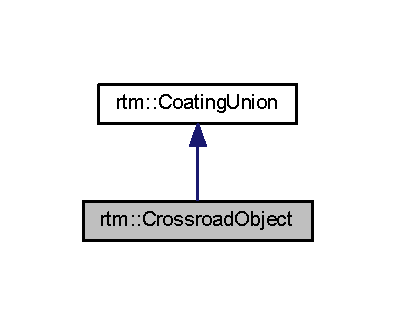
\includegraphics[width=190pt]{classrtm_1_1_crossroad_object__inherit__graph}
\end{center}
\end{figure}
\subsection*{Открытые члены}
\begin{DoxyCompactItemize}
\item 
\mbox{\Hypertarget{classrtm_1_1_crossroad_object_a07fd0e5feeca4e6226dd6043ad9175af}\label{classrtm_1_1_crossroad_object_a07fd0e5feeca4e6226dd6043ad9175af}} 
\hyperlink{classrtm_1_1_crossroad_object_a07fd0e5feeca4e6226dd6043ad9175af}{Crossroad\+Object} ()
\begin{DoxyCompactList}\small\item\em Конструктор по умолчанию \end{DoxyCompactList}\item 
\hyperlink{classrtm_1_1_crossroad_object_a370ec11e5fd53f2191fb107a8fe2a5d5}{Crossroad\+Object} (\hyperlink{namespacertm_aecd3929e64cd461eb3555b611f6fad95}{Coating\+Type} type, int column, int row, \hyperlink{namespacertm_a14457f3088a92b86a96686b72d3e4eea}{Lines\+Counts} lines\+Counts, size\+\_\+t control\+Unit\+Type=0)
\begin{DoxyCompactList}\small\item\em Конструктор для обычного перекрестка \end{DoxyCompactList}\item 
\hyperlink{classrtm_1_1_crossroad_object_a8a76233b7cff3b017ad67bbf5e11a5d3}{Crossroad\+Object} (\hyperlink{namespacertm_aecd3929e64cd461eb3555b611f6fad95}{Coating\+Type} type, int column, int row, \hyperlink{namespacertm_a14457f3088a92b86a96686b72d3e4eea}{Lines\+Counts} lines\+Counts, \hyperlink{namespacertm_a69dc82b16a0148c10962caa83d930f89}{Angle\+Type} null\+Direction, size\+\_\+t control\+Unit\+Type=0)
\begin{DoxyCompactList}\small\item\em Конструктор для Т-\/образного перекрестка \end{DoxyCompactList}\item 
\mbox{\Hypertarget{classrtm_1_1_crossroad_object_a7e004fc5c59d1fd2b2bea0babcd52abe}\label{classrtm_1_1_crossroad_object_a7e004fc5c59d1fd2b2bea0babcd52abe}} 
virtual \hyperlink{classrtm_1_1_crossroad_object_a7e004fc5c59d1fd2b2bea0babcd52abe}{$\sim$\+Crossroad\+Object} ()=default
\begin{DoxyCompactList}\small\item\em Деструктор по умолчанию \end{DoxyCompactList}\item 
\hyperlink{namespacertm_a69dc82b16a0148c10962caa83d930f89}{Angle\+Type} \hyperlink{classrtm_1_1_crossroad_object_a73d0e929640d8aa804122d8e0ab5e961}{Get\+Null\+Direction} () const
\begin{DoxyCompactList}\small\item\em Функция для получения стороны, в направлении которой нельзя двигаться \end{DoxyCompactList}\item 
\hyperlink{namespacertm_a64296d558b2fa02bbf5870afffd61fd9}{Control\+Unit\+Shared} \hyperlink{classrtm_1_1_crossroad_object_a7169a01dc0623fc2701aa184a858be49}{Get\+Control\+Unit} () const
\begin{DoxyCompactList}\small\item\em Функция для получения управляющего блока, привязанного к данному объекту \end{DoxyCompactList}\item 
virtual void \hyperlink{classrtm_1_1_crossroad_object_a2de2a5dac2ba2ca573cfa65a2633de9b}{Show\+Sprites} (cocos2d\+::\+Layer $\ast$const layer) override
\begin{DoxyCompactList}\small\item\em Функция для добавления спрайтов на сцену \end{DoxyCompactList}\item 
virtual void \hyperlink{classrtm_1_1_crossroad_object_a92e9357697edecc69564fd4d40524a3b}{Release\+Sprites} (cocos2d\+::\+Layer $\ast$const layer) override
\begin{DoxyCompactList}\small\item\em Функция для удаления спрайтов со сцены \end{DoxyCompactList}\end{DoxyCompactItemize}
\subsection*{Открытые статические члены}
\begin{DoxyCompactItemize}
\item 
static \hyperlink{namespacertm_ae3bb29510cfde424975be31866d2486e}{Coating\+Matrix} \hyperlink{classrtm_1_1_crossroad_object_a11e6cc77965034adf630b5ac47ab1222}{Crossroad\+Matrix} (\hyperlink{namespacertm_aecd3929e64cd461eb3555b611f6fad95}{Coating\+Type} type, int column, int row, \hyperlink{namespacertm_a14457f3088a92b86a96686b72d3e4eea}{Lines\+Counts} lines\+Counts)
\begin{DoxyCompactList}\small\item\em Функция для получения матрицы покрытий перекрестка \end{DoxyCompactList}\item 
static \hyperlink{namespacertm_ae3bb29510cfde424975be31866d2486e}{Coating\+Matrix} \hyperlink{classrtm_1_1_crossroad_object_a24683882ff8728973a1260ff7acc7a02}{T\+Crossroad\+Matrix} (\hyperlink{namespacertm_aecd3929e64cd461eb3555b611f6fad95}{Coating\+Type} type, int column, int row, \hyperlink{namespacertm_a14457f3088a92b86a96686b72d3e4eea}{Lines\+Counts} lines\+Counts, \hyperlink{namespacertm_a69dc82b16a0148c10962caa83d930f89}{Angle\+Type} null\+Direction)
\begin{DoxyCompactList}\small\item\em Функция для получения матрицы покрытий Т-\/образного перекрестка \end{DoxyCompactList}\end{DoxyCompactItemize}
\subsection*{Закрытые данные}
\begin{DoxyCompactItemize}
\item 
\mbox{\Hypertarget{classrtm_1_1_crossroad_object_a0c335da8c54d6927a9ae1a9a16a908ce}\label{classrtm_1_1_crossroad_object_a0c335da8c54d6927a9ae1a9a16a908ce}} 
\hyperlink{namespacertm_a14457f3088a92b86a96686b72d3e4eea}{Lines\+Counts} \hyperlink{classrtm_1_1_crossroad_object_a0c335da8c54d6927a9ae1a9a16a908ce}{lines\+Counts\+\_\+}
\begin{DoxyCompactList}\small\item\em Количество полос в каждом направлении \end{DoxyCompactList}\item 
\mbox{\Hypertarget{classrtm_1_1_crossroad_object_a8e3056ac82578b7d113d26a4926b6258}\label{classrtm_1_1_crossroad_object_a8e3056ac82578b7d113d26a4926b6258}} 
\hyperlink{namespacertm_a69dc82b16a0148c10962caa83d930f89}{Angle\+Type} \hyperlink{classrtm_1_1_crossroad_object_a8e3056ac82578b7d113d26a4926b6258}{null\+Direction\+\_\+}
\begin{DoxyCompactList}\small\item\em Сторона, в направлении которой нельзя двигаться \end{DoxyCompactList}\item 
\mbox{\Hypertarget{classrtm_1_1_crossroad_object_a77bfe06c0b30c3837cb92e49ce0a5bca}\label{classrtm_1_1_crossroad_object_a77bfe06c0b30c3837cb92e49ce0a5bca}} 
\hyperlink{namespacertm_a64296d558b2fa02bbf5870afffd61fd9}{Control\+Unit\+Shared} \hyperlink{classrtm_1_1_crossroad_object_a77bfe06c0b30c3837cb92e49ce0a5bca}{control\+Unit\+\_\+}
\begin{DoxyCompactList}\small\item\em Умный указатель на управляющий блок \end{DoxyCompactList}\end{DoxyCompactItemize}
\subsection*{Дополнительные унаследованные члены}


\subsection{Подробное описание}
Класс пересечения дорог 

\subsection{Конструктор(ы)}
\mbox{\Hypertarget{classrtm_1_1_crossroad_object_a370ec11e5fd53f2191fb107a8fe2a5d5}\label{classrtm_1_1_crossroad_object_a370ec11e5fd53f2191fb107a8fe2a5d5}} 
\index{rtm\+::\+Crossroad\+Object@{rtm\+::\+Crossroad\+Object}!Crossroad\+Object@{Crossroad\+Object}}
\index{Crossroad\+Object@{Crossroad\+Object}!rtm\+::\+Crossroad\+Object@{rtm\+::\+Crossroad\+Object}}
\subsubsection{\texorpdfstring{Crossroad\+Object()}{CrossroadObject()}\hspace{0.1cm}{\footnotesize\ttfamily [1/2]}}
{\footnotesize\ttfamily rtm\+::\+Crossroad\+Object\+::\+Crossroad\+Object (\begin{DoxyParamCaption}\item[{\hyperlink{namespacertm_aecd3929e64cd461eb3555b611f6fad95}{Coating\+Type}}]{type,  }\item[{int}]{column,  }\item[{int}]{row,  }\item[{\hyperlink{namespacertm_a14457f3088a92b86a96686b72d3e4eea}{Lines\+Counts}}]{lines\+Counts,  }\item[{size\+\_\+t}]{control\+Unit\+Type = {\ttfamily 0} }\end{DoxyParamCaption})}



Конструктор для обычного перекрестка 


\begin{DoxyParams}{Аргументы}
{\em type} & тип покрытия \\
\hline
{\em column} & левая колонка перекрестка \\
\hline
{\em row} & нижняя строка перекрестка \\
\hline
{\em lines\+Counts} & количество полос в каждом направлении \\
\hline
{\em control\+Unit\+Type} & номер типа управляющего блока \\
\hline
\end{DoxyParams}
\mbox{\Hypertarget{classrtm_1_1_crossroad_object_a8a76233b7cff3b017ad67bbf5e11a5d3}\label{classrtm_1_1_crossroad_object_a8a76233b7cff3b017ad67bbf5e11a5d3}} 
\index{rtm\+::\+Crossroad\+Object@{rtm\+::\+Crossroad\+Object}!Crossroad\+Object@{Crossroad\+Object}}
\index{Crossroad\+Object@{Crossroad\+Object}!rtm\+::\+Crossroad\+Object@{rtm\+::\+Crossroad\+Object}}
\subsubsection{\texorpdfstring{Crossroad\+Object()}{CrossroadObject()}\hspace{0.1cm}{\footnotesize\ttfamily [2/2]}}
{\footnotesize\ttfamily rtm\+::\+Crossroad\+Object\+::\+Crossroad\+Object (\begin{DoxyParamCaption}\item[{\hyperlink{namespacertm_aecd3929e64cd461eb3555b611f6fad95}{Coating\+Type}}]{type,  }\item[{int}]{column,  }\item[{int}]{row,  }\item[{\hyperlink{namespacertm_a14457f3088a92b86a96686b72d3e4eea}{Lines\+Counts}}]{lines\+Counts,  }\item[{\hyperlink{namespacertm_a69dc82b16a0148c10962caa83d930f89}{Angle\+Type}}]{null\+Direction,  }\item[{size\+\_\+t}]{control\+Unit\+Type = {\ttfamily 0} }\end{DoxyParamCaption})}



Конструктор для Т-\/образного перекрестка 


\begin{DoxyParams}{Аргументы}
{\em type} & тип покрытия \\
\hline
{\em column} & левая колонка перекрестка \\
\hline
{\em row} & нижняя строка перекрестка \\
\hline
{\em lines\+Counts} & количество полос в каждом направлении \\
\hline
{\em null\+Direction} & сторона, в направлении которой нельзя двигаться \\
\hline
{\em control\+Unit\+Type} & номер типа управляющего блока \\
\hline
\end{DoxyParams}


\subsection{Методы}
\mbox{\Hypertarget{classrtm_1_1_crossroad_object_a11e6cc77965034adf630b5ac47ab1222}\label{classrtm_1_1_crossroad_object_a11e6cc77965034adf630b5ac47ab1222}} 
\index{rtm\+::\+Crossroad\+Object@{rtm\+::\+Crossroad\+Object}!Crossroad\+Matrix@{Crossroad\+Matrix}}
\index{Crossroad\+Matrix@{Crossroad\+Matrix}!rtm\+::\+Crossroad\+Object@{rtm\+::\+Crossroad\+Object}}
\subsubsection{\texorpdfstring{Crossroad\+Matrix()}{CrossroadMatrix()}}
{\footnotesize\ttfamily \hyperlink{namespacertm_ae3bb29510cfde424975be31866d2486e}{rtm\+::\+Coating\+Matrix} rtm\+::\+Crossroad\+Object\+::\+Crossroad\+Matrix (\begin{DoxyParamCaption}\item[{\hyperlink{namespacertm_aecd3929e64cd461eb3555b611f6fad95}{Coating\+Type}}]{type,  }\item[{int}]{column,  }\item[{int}]{row,  }\item[{\hyperlink{namespacertm_a14457f3088a92b86a96686b72d3e4eea}{Lines\+Counts}}]{lines\+Counts }\end{DoxyParamCaption})\hspace{0.3cm}{\ttfamily [static]}}



Функция для получения матрицы покрытий перекрестка 


\begin{DoxyParams}{Аргументы}
{\em type} & тип покрытия \\
\hline
{\em column} & левая колонка перекрестка \\
\hline
{\em row} & нижняя строка перекрестка \\
\hline
{\em lines\+Counts} & количество полос в каждом направлении \\
\hline
\end{DoxyParams}
\begin{DoxyReturn}{Возвращает}
матрица покрытий 
\end{DoxyReturn}
\mbox{\Hypertarget{classrtm_1_1_crossroad_object_a24683882ff8728973a1260ff7acc7a02}\label{classrtm_1_1_crossroad_object_a24683882ff8728973a1260ff7acc7a02}} 
\index{rtm\+::\+Crossroad\+Object@{rtm\+::\+Crossroad\+Object}!T\+Crossroad\+Matrix@{T\+Crossroad\+Matrix}}
\index{T\+Crossroad\+Matrix@{T\+Crossroad\+Matrix}!rtm\+::\+Crossroad\+Object@{rtm\+::\+Crossroad\+Object}}
\subsubsection{\texorpdfstring{T\+Crossroad\+Matrix()}{TCrossroadMatrix()}}
{\footnotesize\ttfamily \hyperlink{namespacertm_ae3bb29510cfde424975be31866d2486e}{rtm\+::\+Coating\+Matrix} rtm\+::\+Crossroad\+Object\+::\+T\+Crossroad\+Matrix (\begin{DoxyParamCaption}\item[{\hyperlink{namespacertm_aecd3929e64cd461eb3555b611f6fad95}{Coating\+Type}}]{type,  }\item[{int}]{column,  }\item[{int}]{row,  }\item[{\hyperlink{namespacertm_a14457f3088a92b86a96686b72d3e4eea}{Lines\+Counts}}]{lines\+Counts,  }\item[{\hyperlink{namespacertm_a69dc82b16a0148c10962caa83d930f89}{Angle\+Type}}]{null\+Direction }\end{DoxyParamCaption})\hspace{0.3cm}{\ttfamily [static]}}



Функция для получения матрицы покрытий Т-\/образного перекрестка 


\begin{DoxyParams}{Аргументы}
{\em type} & тип покрытия \\
\hline
{\em column} & левая колонка перекрестка \\
\hline
{\em row} & нижняя строка перекрестка \\
\hline
{\em lines\+Counts} & количество полос в каждом направлении \\
\hline
{\em null\+Direction} & сторона, в направлении которой нельзя двигаться \\
\hline
\end{DoxyParams}
\begin{DoxyReturn}{Возвращает}
матрица покрытий 
\end{DoxyReturn}
\mbox{\Hypertarget{classrtm_1_1_crossroad_object_a73d0e929640d8aa804122d8e0ab5e961}\label{classrtm_1_1_crossroad_object_a73d0e929640d8aa804122d8e0ab5e961}} 
\index{rtm\+::\+Crossroad\+Object@{rtm\+::\+Crossroad\+Object}!Get\+Null\+Direction@{Get\+Null\+Direction}}
\index{Get\+Null\+Direction@{Get\+Null\+Direction}!rtm\+::\+Crossroad\+Object@{rtm\+::\+Crossroad\+Object}}
\subsubsection{\texorpdfstring{Get\+Null\+Direction()}{GetNullDirection()}}
{\footnotesize\ttfamily \hyperlink{namespacertm_a69dc82b16a0148c10962caa83d930f89}{rtm\+::\+Angle\+Type} rtm\+::\+Crossroad\+Object\+::\+Get\+Null\+Direction (\begin{DoxyParamCaption}{ }\end{DoxyParamCaption}) const}



Функция для получения стороны, в направлении которой нельзя двигаться 

\begin{DoxyReturn}{Возвращает}
угол, соответствующий запрещенной стороне 
\end{DoxyReturn}
\mbox{\Hypertarget{classrtm_1_1_crossroad_object_a7169a01dc0623fc2701aa184a858be49}\label{classrtm_1_1_crossroad_object_a7169a01dc0623fc2701aa184a858be49}} 
\index{rtm\+::\+Crossroad\+Object@{rtm\+::\+Crossroad\+Object}!Get\+Control\+Unit@{Get\+Control\+Unit}}
\index{Get\+Control\+Unit@{Get\+Control\+Unit}!rtm\+::\+Crossroad\+Object@{rtm\+::\+Crossroad\+Object}}
\subsubsection{\texorpdfstring{Get\+Control\+Unit()}{GetControlUnit()}}
{\footnotesize\ttfamily \hyperlink{namespacertm_a64296d558b2fa02bbf5870afffd61fd9}{rtm\+::\+Control\+Unit\+Shared} rtm\+::\+Crossroad\+Object\+::\+Get\+Control\+Unit (\begin{DoxyParamCaption}{ }\end{DoxyParamCaption}) const}



Функция для получения управляющего блока, привязанного к данному объекту 

\begin{DoxyReturn}{Возвращает}
умный указатель на управляющий блок 
\end{DoxyReturn}
\mbox{\Hypertarget{classrtm_1_1_crossroad_object_a2de2a5dac2ba2ca573cfa65a2633de9b}\label{classrtm_1_1_crossroad_object_a2de2a5dac2ba2ca573cfa65a2633de9b}} 
\index{rtm\+::\+Crossroad\+Object@{rtm\+::\+Crossroad\+Object}!Show\+Sprites@{Show\+Sprites}}
\index{Show\+Sprites@{Show\+Sprites}!rtm\+::\+Crossroad\+Object@{rtm\+::\+Crossroad\+Object}}
\subsubsection{\texorpdfstring{Show\+Sprites()}{ShowSprites()}}
{\footnotesize\ttfamily void rtm\+::\+Crossroad\+Object\+::\+Show\+Sprites (\begin{DoxyParamCaption}\item[{cocos2d\+::\+Layer $\ast$const}]{layer }\end{DoxyParamCaption})\hspace{0.3cm}{\ttfamily [override]}, {\ttfamily [virtual]}}



Функция для добавления спрайтов на сцену 


\begin{DoxyParams}{Аргументы}
{\em layer} & слой, на который надо добавить спрайты управляющего блока \\
\hline
\end{DoxyParams}


Переопределяет метод предка \hyperlink{classrtm_1_1_coating_union_ae95be187677aec759723edb4d14b35c1}{rtm\+::\+Coating\+Union}.

\mbox{\Hypertarget{classrtm_1_1_crossroad_object_a92e9357697edecc69564fd4d40524a3b}\label{classrtm_1_1_crossroad_object_a92e9357697edecc69564fd4d40524a3b}} 
\index{rtm\+::\+Crossroad\+Object@{rtm\+::\+Crossroad\+Object}!Release\+Sprites@{Release\+Sprites}}
\index{Release\+Sprites@{Release\+Sprites}!rtm\+::\+Crossroad\+Object@{rtm\+::\+Crossroad\+Object}}
\subsubsection{\texorpdfstring{Release\+Sprites()}{ReleaseSprites()}}
{\footnotesize\ttfamily void rtm\+::\+Crossroad\+Object\+::\+Release\+Sprites (\begin{DoxyParamCaption}\item[{cocos2d\+::\+Layer $\ast$const}]{layer }\end{DoxyParamCaption})\hspace{0.3cm}{\ttfamily [override]}, {\ttfamily [virtual]}}



Функция для удаления спрайтов со сцены 


\begin{DoxyParams}{Аргументы}
{\em layer} & слой, с которого надо удалить спрайты управляющего блока \\
\hline
\end{DoxyParams}


Переопределяет метод предка \hyperlink{classrtm_1_1_coating_union_a4e046aae25ce91da0408ac31a0de4e21}{rtm\+::\+Coating\+Union}.



Объявления и описания членов классов находятся в файлах\+:\begin{DoxyCompactItemize}
\item 
C\+:/\+Users/\+Vladimir/\+Documents/\+Visual Studio 2017/\+Projects/\+R\+T\+M/\+Classes/Crossroad\+Object.\+h\item 
C\+:/\+Users/\+Vladimir/\+Documents/\+Visual Studio 2017/\+Projects/\+R\+T\+M/\+Classes/Crossroad\+Object.\+cpp\end{DoxyCompactItemize}

\hypertarget{classrtm_1_1_driveway_object}{}\section{Класс rtm\+:\+:Driveway\+Object}
\label{classrtm_1_1_driveway_object}\index{rtm\+::\+Driveway\+Object@{rtm\+::\+Driveway\+Object}}


Класс прямой дороги  




{\ttfamily \#include $<$Driveway\+Object.\+h$>$}



Граф наследования\+:rtm\+:\+:Driveway\+Object\+:
\nopagebreak
\begin{figure}[H]
\begin{center}
\leavevmode
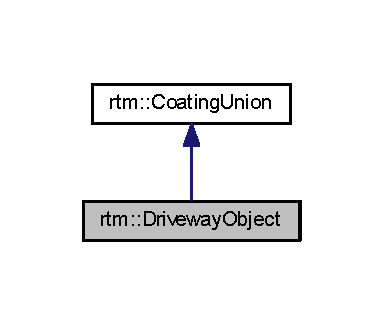
\includegraphics[width=184pt]{classrtm_1_1_driveway_object__inherit__graph}
\end{center}
\end{figure}
\subsection*{Открытые члены}
\begin{DoxyCompactItemize}
\item 
\mbox{\Hypertarget{classrtm_1_1_driveway_object_a0db985799ef0297057c2e33284418a6b}\label{classrtm_1_1_driveway_object_a0db985799ef0297057c2e33284418a6b}} 
\hyperlink{classrtm_1_1_driveway_object_a0db985799ef0297057c2e33284418a6b}{Driveway\+Object} ()
\begin{DoxyCompactList}\small\item\em Конструктор по умолчанию \end{DoxyCompactList}\item 
\hyperlink{classrtm_1_1_driveway_object_aa9f5531382b6be2c6fb0cde4160a9f90}{Driveway\+Object} (\hyperlink{namespacertm_aecd3929e64cd461eb3555b611f6fad95}{Coating\+Type} type, int column, int row, size\+\_\+t width, size\+\_\+t height, \hyperlink{namespacertm_a69dc82b16a0148c10962caa83d930f89}{Angle\+Type} angle)
\item 
\mbox{\Hypertarget{classrtm_1_1_driveway_object_a822b655b5c429ce2775a3999f77265a0}\label{classrtm_1_1_driveway_object_a822b655b5c429ce2775a3999f77265a0}} 
virtual \hyperlink{classrtm_1_1_driveway_object_a822b655b5c429ce2775a3999f77265a0}{$\sim$\+Driveway\+Object} ()=default
\begin{DoxyCompactList}\small\item\em Деструктор по умолчанию \end{DoxyCompactList}\item 
virtual float \hyperlink{classrtm_1_1_driveway_object_a5de41ef395ad8ccefb435e568f84ed40}{Get\+Length} () const override
\item 
size\+\_\+t \hyperlink{classrtm_1_1_driveway_object_a239d7f4d9d5203d1f00cf60294e94151}{Get\+Lines\+Count} () const
\item 
bool \hyperlink{classrtm_1_1_driveway_object_ae427989fc802b24d06f6b7f83959be2a}{is\+Right\+Line} (int column, int row) const
\item 
bool \hyperlink{classrtm_1_1_driveway_object_addaa5faebb5469e8074a46f6c3584e56}{is\+Right\+Line} (float x, float y) const
\item 
bool \hyperlink{classrtm_1_1_driveway_object_aea7d711c9cf1ba995bc08d805373cc52}{is\+Left\+Line} (int column, int row) const
\item 
bool \hyperlink{classrtm_1_1_driveway_object_afa48600b7d87a38e6c690e3b1058d177}{is\+Left\+Line} (float x, float y) const
\end{DoxyCompactItemize}
\subsection*{Открытые статические члены}
\begin{DoxyCompactItemize}
\item 
static \hyperlink{namespacertm_ae3bb29510cfde424975be31866d2486e}{Coating\+Matrix} \hyperlink{classrtm_1_1_driveway_object_ab89dd0516cf883cb0c3332ae0bbc1726}{Driveway\+Matrix} (\hyperlink{namespacertm_aecd3929e64cd461eb3555b611f6fad95}{Coating\+Type} type, int column, int row, size\+\_\+t width, size\+\_\+t height, \hyperlink{namespacertm_a69dc82b16a0148c10962caa83d930f89}{Angle\+Type} angle)
\end{DoxyCompactItemize}
\subsection*{Закрытые статические члены}
\begin{DoxyCompactItemize}
\item 
static float \hyperlink{classrtm_1_1_driveway_object_a6ebdc5c00005dbc2e96243767ba33273}{Count\+Length\+\_\+} (size\+\_\+t width, size\+\_\+t height, \hyperlink{namespacertm_a69dc82b16a0148c10962caa83d930f89}{Angle\+Type} angle)
\item 
static size\+\_\+t \hyperlink{classrtm_1_1_driveway_object_af8a26a955200fde09d68d606a68c5f8c}{Count\+Lines\+\_\+} (size\+\_\+t width, size\+\_\+t height, \hyperlink{namespacertm_a69dc82b16a0148c10962caa83d930f89}{Angle\+Type} angle)
\end{DoxyCompactItemize}
\subsection*{Закрытые данные}
\begin{DoxyCompactItemize}
\item 
\mbox{\Hypertarget{classrtm_1_1_driveway_object_ae1a5ce1c3e82307f34c1d31ad004b075}\label{classrtm_1_1_driveway_object_ae1a5ce1c3e82307f34c1d31ad004b075}} 
\hyperlink{namespacertm_a69dc82b16a0148c10962caa83d930f89}{Angle\+Type} \hyperlink{classrtm_1_1_driveway_object_ae1a5ce1c3e82307f34c1d31ad004b075}{angle\+\_\+}
\begin{DoxyCompactList}\small\item\em Направление движения \end{DoxyCompactList}\item 
\mbox{\Hypertarget{classrtm_1_1_driveway_object_a7338ac80dc7ac9e9a9f109c57fa1ff20}\label{classrtm_1_1_driveway_object_a7338ac80dc7ac9e9a9f109c57fa1ff20}} 
float \hyperlink{classrtm_1_1_driveway_object_a7338ac80dc7ac9e9a9f109c57fa1ff20}{length\+\_\+}
\begin{DoxyCompactList}\small\item\em Длина объекта (для вычисления кратчайшего пути) \end{DoxyCompactList}\item 
\mbox{\Hypertarget{classrtm_1_1_driveway_object_acb732900dd6a079b71038f3bb8732818}\label{classrtm_1_1_driveway_object_acb732900dd6a079b71038f3bb8732818}} 
size\+\_\+t \hyperlink{classrtm_1_1_driveway_object_acb732900dd6a079b71038f3bb8732818}{lines\+Count\+\_\+}
\begin{DoxyCompactList}\small\item\em Количество полос \end{DoxyCompactList}\end{DoxyCompactItemize}
\subsection*{Дополнительные унаследованные члены}


\subsection{Подробное описание}
Класс прямой дороги 

\subsection{Конструктор(ы)}
\mbox{\Hypertarget{classrtm_1_1_driveway_object_aa9f5531382b6be2c6fb0cde4160a9f90}\label{classrtm_1_1_driveway_object_aa9f5531382b6be2c6fb0cde4160a9f90}} 
\index{rtm\+::\+Driveway\+Object@{rtm\+::\+Driveway\+Object}!Driveway\+Object@{Driveway\+Object}}
\index{Driveway\+Object@{Driveway\+Object}!rtm\+::\+Driveway\+Object@{rtm\+::\+Driveway\+Object}}
\subsubsection{\texorpdfstring{Driveway\+Object()}{DrivewayObject()}}
{\footnotesize\ttfamily rtm\+::\+Driveway\+Object\+::\+Driveway\+Object (\begin{DoxyParamCaption}\item[{\hyperlink{namespacertm_aecd3929e64cd461eb3555b611f6fad95}{Coating\+Type}}]{type,  }\item[{int}]{column,  }\item[{int}]{row,  }\item[{size\+\_\+t}]{width,  }\item[{size\+\_\+t}]{height,  }\item[{\hyperlink{namespacertm_a69dc82b16a0148c10962caa83d930f89}{Angle\+Type}}]{angle }\end{DoxyParamCaption})}

Конструктор по размерам 
\begin{DoxyParams}{Аргументы}
{\em type} & тип покрытия \\
\hline
{\em column} & левая колонка объекта \\
\hline
{\em row} & нижняя строка объекта \\
\hline
{\em width} & ширина объекта \\
\hline
{\em height} & высота объекта \\
\hline
{\em angle} & направление движения \\
\hline
\end{DoxyParams}


\subsection{Методы}
\mbox{\Hypertarget{classrtm_1_1_driveway_object_ab89dd0516cf883cb0c3332ae0bbc1726}\label{classrtm_1_1_driveway_object_ab89dd0516cf883cb0c3332ae0bbc1726}} 
\index{rtm\+::\+Driveway\+Object@{rtm\+::\+Driveway\+Object}!Driveway\+Matrix@{Driveway\+Matrix}}
\index{Driveway\+Matrix@{Driveway\+Matrix}!rtm\+::\+Driveway\+Object@{rtm\+::\+Driveway\+Object}}
\subsubsection{\texorpdfstring{Driveway\+Matrix()}{DrivewayMatrix()}}
{\footnotesize\ttfamily \hyperlink{namespacertm_ae3bb29510cfde424975be31866d2486e}{rtm\+::\+Coating\+Matrix} rtm\+::\+Driveway\+Object\+::\+Driveway\+Matrix (\begin{DoxyParamCaption}\item[{\hyperlink{namespacertm_aecd3929e64cd461eb3555b611f6fad95}{Coating\+Type}}]{type,  }\item[{int}]{column,  }\item[{int}]{row,  }\item[{size\+\_\+t}]{width,  }\item[{size\+\_\+t}]{height,  }\item[{\hyperlink{namespacertm_a69dc82b16a0148c10962caa83d930f89}{Angle\+Type}}]{angle }\end{DoxyParamCaption})\hspace{0.3cm}{\ttfamily [static]}}

Функция для получения матрицы покрытий дороги 
\begin{DoxyParams}{Аргументы}
{\em type} & тип покрытия \\
\hline
{\em column} & левая колонка объекта \\
\hline
{\em row} & нижняя строка объекта \\
\hline
{\em width} & ширина объекта \\
\hline
{\em height} & высота объекта \\
\hline
{\em angle} & направление движения \\
\hline
\end{DoxyParams}
\begin{DoxyReturn}{Возвращает}
матрица покрытий 
\end{DoxyReturn}
\mbox{\Hypertarget{classrtm_1_1_driveway_object_a5de41ef395ad8ccefb435e568f84ed40}\label{classrtm_1_1_driveway_object_a5de41ef395ad8ccefb435e568f84ed40}} 
\index{rtm\+::\+Driveway\+Object@{rtm\+::\+Driveway\+Object}!Get\+Length@{Get\+Length}}
\index{Get\+Length@{Get\+Length}!rtm\+::\+Driveway\+Object@{rtm\+::\+Driveway\+Object}}
\subsubsection{\texorpdfstring{Get\+Length()}{GetLength()}}
{\footnotesize\ttfamily float rtm\+::\+Driveway\+Object\+::\+Get\+Length (\begin{DoxyParamCaption}{ }\end{DoxyParamCaption}) const\hspace{0.3cm}{\ttfamily [override]}, {\ttfamily [virtual]}}

Функция для получения длины объекта (для вычисления кратчайшего пути) \begin{DoxyReturn}{Возвращает}
длина 
\end{DoxyReturn}


Переопределяет метод предка \hyperlink{classrtm_1_1_coating_union_adf3ec4f4e8399c455aaa73bfe726b4ce}{rtm\+::\+Coating\+Union}.

\mbox{\Hypertarget{classrtm_1_1_driveway_object_a239d7f4d9d5203d1f00cf60294e94151}\label{classrtm_1_1_driveway_object_a239d7f4d9d5203d1f00cf60294e94151}} 
\index{rtm\+::\+Driveway\+Object@{rtm\+::\+Driveway\+Object}!Get\+Lines\+Count@{Get\+Lines\+Count}}
\index{Get\+Lines\+Count@{Get\+Lines\+Count}!rtm\+::\+Driveway\+Object@{rtm\+::\+Driveway\+Object}}
\subsubsection{\texorpdfstring{Get\+Lines\+Count()}{GetLinesCount()}}
{\footnotesize\ttfamily size\+\_\+t rtm\+::\+Driveway\+Object\+::\+Get\+Lines\+Count (\begin{DoxyParamCaption}{ }\end{DoxyParamCaption}) const}

Функция для получения количества полос \begin{DoxyReturn}{Возвращает}
количество полос 
\end{DoxyReturn}
\mbox{\Hypertarget{classrtm_1_1_driveway_object_ae427989fc802b24d06f6b7f83959be2a}\label{classrtm_1_1_driveway_object_ae427989fc802b24d06f6b7f83959be2a}} 
\index{rtm\+::\+Driveway\+Object@{rtm\+::\+Driveway\+Object}!is\+Right\+Line@{is\+Right\+Line}}
\index{is\+Right\+Line@{is\+Right\+Line}!rtm\+::\+Driveway\+Object@{rtm\+::\+Driveway\+Object}}
\subsubsection{\texorpdfstring{is\+Right\+Line()}{isRightLine()}\hspace{0.1cm}{\footnotesize\ttfamily [1/2]}}
{\footnotesize\ttfamily bool rtm\+::\+Driveway\+Object\+::is\+Right\+Line (\begin{DoxyParamCaption}\item[{int}]{column,  }\item[{int}]{row }\end{DoxyParamCaption}) const}

Функция для проверки\+: находится ли объект в правой полосе 
\begin{DoxyParams}{Аргументы}
{\em column} & колонка, в которой находится объект \\
\hline
{\em row} & строка, в которой находится объект \\
\hline
\end{DoxyParams}
\begin{DoxyReturn}{Возвращает}
true, если объект находится в правой полосе, иначе false 
\end{DoxyReturn}
\mbox{\Hypertarget{classrtm_1_1_driveway_object_addaa5faebb5469e8074a46f6c3584e56}\label{classrtm_1_1_driveway_object_addaa5faebb5469e8074a46f6c3584e56}} 
\index{rtm\+::\+Driveway\+Object@{rtm\+::\+Driveway\+Object}!is\+Right\+Line@{is\+Right\+Line}}
\index{is\+Right\+Line@{is\+Right\+Line}!rtm\+::\+Driveway\+Object@{rtm\+::\+Driveway\+Object}}
\subsubsection{\texorpdfstring{is\+Right\+Line()}{isRightLine()}\hspace{0.1cm}{\footnotesize\ttfamily [2/2]}}
{\footnotesize\ttfamily bool rtm\+::\+Driveway\+Object\+::is\+Right\+Line (\begin{DoxyParamCaption}\item[{float}]{x,  }\item[{float}]{y }\end{DoxyParamCaption}) const}

Функция для проверки\+: находится ли объект в правой полосе 
\begin{DoxyParams}{Аргументы}
{\em x} & абсцисса объекта \\
\hline
{\em y} & ордината объекта \\
\hline
\end{DoxyParams}
\begin{DoxyReturn}{Возвращает}
true, если объект находится в правой полосе, иначе false 
\end{DoxyReturn}
\mbox{\Hypertarget{classrtm_1_1_driveway_object_aea7d711c9cf1ba995bc08d805373cc52}\label{classrtm_1_1_driveway_object_aea7d711c9cf1ba995bc08d805373cc52}} 
\index{rtm\+::\+Driveway\+Object@{rtm\+::\+Driveway\+Object}!is\+Left\+Line@{is\+Left\+Line}}
\index{is\+Left\+Line@{is\+Left\+Line}!rtm\+::\+Driveway\+Object@{rtm\+::\+Driveway\+Object}}
\subsubsection{\texorpdfstring{is\+Left\+Line()}{isLeftLine()}\hspace{0.1cm}{\footnotesize\ttfamily [1/2]}}
{\footnotesize\ttfamily bool rtm\+::\+Driveway\+Object\+::is\+Left\+Line (\begin{DoxyParamCaption}\item[{int}]{column,  }\item[{int}]{row }\end{DoxyParamCaption}) const}

Функция для проверки\+: находится ли объект в левой полосе 
\begin{DoxyParams}{Аргументы}
{\em column} & колонка, в которой находится объект \\
\hline
{\em row} & строка, в которой находится объект \\
\hline
\end{DoxyParams}
\begin{DoxyReturn}{Возвращает}
true, если объект находится в левой полосе, иначе false 
\end{DoxyReturn}
\mbox{\Hypertarget{classrtm_1_1_driveway_object_afa48600b7d87a38e6c690e3b1058d177}\label{classrtm_1_1_driveway_object_afa48600b7d87a38e6c690e3b1058d177}} 
\index{rtm\+::\+Driveway\+Object@{rtm\+::\+Driveway\+Object}!is\+Left\+Line@{is\+Left\+Line}}
\index{is\+Left\+Line@{is\+Left\+Line}!rtm\+::\+Driveway\+Object@{rtm\+::\+Driveway\+Object}}
\subsubsection{\texorpdfstring{is\+Left\+Line()}{isLeftLine()}\hspace{0.1cm}{\footnotesize\ttfamily [2/2]}}
{\footnotesize\ttfamily bool rtm\+::\+Driveway\+Object\+::is\+Left\+Line (\begin{DoxyParamCaption}\item[{float}]{x,  }\item[{float}]{y }\end{DoxyParamCaption}) const}

Функция для проверки\+: находится ли объект в левой полосе 
\begin{DoxyParams}{Аргументы}
{\em x} & абсцисса объекта \\
\hline
{\em y} & ордината объекта \\
\hline
\end{DoxyParams}
\begin{DoxyReturn}{Возвращает}
true, если объект находится в левой полосе, иначе false 
\end{DoxyReturn}
\mbox{\Hypertarget{classrtm_1_1_driveway_object_a6ebdc5c00005dbc2e96243767ba33273}\label{classrtm_1_1_driveway_object_a6ebdc5c00005dbc2e96243767ba33273}} 
\index{rtm\+::\+Driveway\+Object@{rtm\+::\+Driveway\+Object}!Count\+Length\+\_\+@{Count\+Length\+\_\+}}
\index{Count\+Length\+\_\+@{Count\+Length\+\_\+}!rtm\+::\+Driveway\+Object@{rtm\+::\+Driveway\+Object}}
\subsubsection{\texorpdfstring{Count\+Length\+\_\+()}{CountLength\_()}}
{\footnotesize\ttfamily float rtm\+::\+Driveway\+Object\+::\+Count\+Length\+\_\+ (\begin{DoxyParamCaption}\item[{size\+\_\+t}]{width,  }\item[{size\+\_\+t}]{height,  }\item[{\hyperlink{namespacertm_a69dc82b16a0148c10962caa83d930f89}{Angle\+Type}}]{angle }\end{DoxyParamCaption})\hspace{0.3cm}{\ttfamily [static]}, {\ttfamily [private]}}

Функция для вычисления длины объекта 
\begin{DoxyParams}{Аргументы}
{\em width} & ширина объекта \\
\hline
{\em height} & высота объекта \\
\hline
{\em angle} & направление движения \\
\hline
\end{DoxyParams}
\begin{DoxyReturn}{Возвращает}
длина объекта 
\end{DoxyReturn}
\mbox{\Hypertarget{classrtm_1_1_driveway_object_af8a26a955200fde09d68d606a68c5f8c}\label{classrtm_1_1_driveway_object_af8a26a955200fde09d68d606a68c5f8c}} 
\index{rtm\+::\+Driveway\+Object@{rtm\+::\+Driveway\+Object}!Count\+Lines\+\_\+@{Count\+Lines\+\_\+}}
\index{Count\+Lines\+\_\+@{Count\+Lines\+\_\+}!rtm\+::\+Driveway\+Object@{rtm\+::\+Driveway\+Object}}
\subsubsection{\texorpdfstring{Count\+Lines\+\_\+()}{CountLines\_()}}
{\footnotesize\ttfamily size\+\_\+t rtm\+::\+Driveway\+Object\+::\+Count\+Lines\+\_\+ (\begin{DoxyParamCaption}\item[{size\+\_\+t}]{width,  }\item[{size\+\_\+t}]{height,  }\item[{\hyperlink{namespacertm_a69dc82b16a0148c10962caa83d930f89}{Angle\+Type}}]{angle }\end{DoxyParamCaption})\hspace{0.3cm}{\ttfamily [static]}, {\ttfamily [private]}}

Функция для получения количества полос 
\begin{DoxyParams}{Аргументы}
{\em width} & ширина объекта \\
\hline
{\em height} & высота объекта \\
\hline
{\em angle} & направление движения \\
\hline
\end{DoxyParams}
\begin{DoxyReturn}{Возвращает}
количество полос 
\end{DoxyReturn}


Объявления и описания членов классов находятся в файлах\+:\begin{DoxyCompactItemize}
\item 
C\+:/\+Users/\+Vladimir/\+Documents/\+Visual Studio 2017/\+Projects/\+R\+T\+M/\+Classes/Driveway\+Object.\+h\item 
C\+:/\+Users/\+Vladimir/\+Documents/\+Visual Studio 2017/\+Projects/\+R\+T\+M/\+Classes/Driveway\+Object.\+cpp\end{DoxyCompactItemize}

\hypertarget{classrtm_1_1_dynamic_object}{}\section{Класс rtm\+:\+:Dynamic\+Object}
\label{classrtm_1_1_dynamic_object}\index{rtm\+::\+Dynamic\+Object@{rtm\+::\+Dynamic\+Object}}


Класс динамического объекта (который двигается, обновляется)  




{\ttfamily \#include $<$Dynamic\+Object.\+h$>$}



Граф наследования\+:rtm\+:\+:Dynamic\+Object\+:
\nopagebreak
\begin{figure}[H]
\begin{center}
\leavevmode
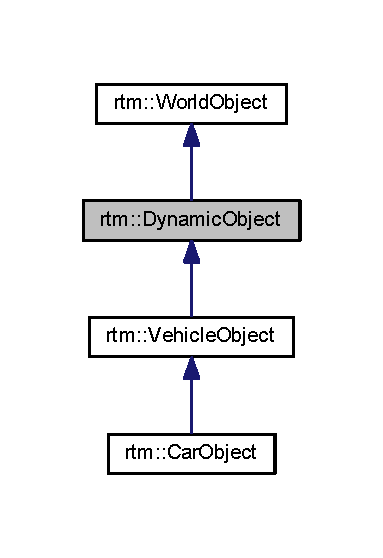
\includegraphics[width=184pt]{classrtm_1_1_dynamic_object__inherit__graph}
\end{center}
\end{figure}
\subsection*{Открытые члены}
\begin{DoxyCompactItemize}
\item 
\mbox{\Hypertarget{classrtm_1_1_dynamic_object_aeb59f3ec97c939c5b12a8738206557c2}\label{classrtm_1_1_dynamic_object_aeb59f3ec97c939c5b12a8738206557c2}} 
\hyperlink{classrtm_1_1_dynamic_object_aeb59f3ec97c939c5b12a8738206557c2}{Dynamic\+Object} ()
\begin{DoxyCompactList}\small\item\em Конструктор по умочанию \end{DoxyCompactList}\item 
\hyperlink{classrtm_1_1_dynamic_object_a404c2232fe49bb759fd6a473d74131ed}{Dynamic\+Object} (cocos2d\+::\+Sprite $\ast$sprite, float x, float y, float angle, float speed)
\item 
\hyperlink{classrtm_1_1_dynamic_object_aa65c16292e48449c981ed3710d7a6a26}{Dynamic\+Object} (std\+::string const \&filename, float x, float y, float angle, float speed)
\item 
\mbox{\Hypertarget{classrtm_1_1_dynamic_object_ae98f1897c1299f8f0aa2d4994e23090a}\label{classrtm_1_1_dynamic_object_ae98f1897c1299f8f0aa2d4994e23090a}} 
virtual \hyperlink{classrtm_1_1_dynamic_object_ae98f1897c1299f8f0aa2d4994e23090a}{$\sim$\+Dynamic\+Object} ()=default
\begin{DoxyCompactList}\small\item\em Деструктор по умолчанию \end{DoxyCompactList}\item 
float \hyperlink{classrtm_1_1_dynamic_object_ac75970216f8be37f7b5eefd1f506215f}{Get\+Speed} () const
\item 
float \hyperlink{classrtm_1_1_dynamic_object_ada2fd3defc1cea052020023b99be12ec}{Get\+Last\+Delta} () const
\item 
bool \hyperlink{classrtm_1_1_dynamic_object_a0bc9390b78faf5c770bff86a2e451ec6}{Has\+Collision} () const
\item 
virtual void \hyperlink{classrtm_1_1_dynamic_object_a2b2a4072f80d6be9c8d1097bc072197e}{Update} (\hyperlink{classrtm_1_1_world_controller}{World\+Controller} $\ast$const world)
\item 
bool \hyperlink{classrtm_1_1_dynamic_object_adcbb0baaad8ba2185e00221cc90fdee9}{Is\+Near\+Others} (\hyperlink{classrtm_1_1_world_controller}{World\+Controller} $\ast$const world)
\end{DoxyCompactItemize}
\subsection*{Защищенные члены}
\begin{DoxyCompactItemize}
\item 
void \hyperlink{classrtm_1_1_dynamic_object_aceb38c6ff9d41d814953d4538e32542f}{Set\+Speed\+\_\+} (float speed)
\item 
void \hyperlink{classrtm_1_1_dynamic_object_a50d64daac674d1e9f55ce1fb73cf9d6a}{Set\+Collision\+Flag\+\_\+} (bool flag)
\item 
bool \hyperlink{classrtm_1_1_dynamic_object_a8ed34444a34b29ff9a672839c6593558}{Is\+Beholding\+\_\+} (\hyperlink{classrtm_1_1_world_object}{World\+Object} const $\ast$const other, float radius=\hyperlink{namespacertm_a6ae2631935a995c34abce1c62fa3dcd7}{V\+I\+E\+W\+\_\+\+R\+A\+D\+I\+US}, float angle=\hyperlink{namespacertm_af0ecac808d3938e77a20990f1947c8fd}{V\+I\+E\+W\+\_\+\+A\+N\+G\+LE}, float angle\+Shift=\hyperlink{namespacertm_a10eed490bb183c7853ac317d82e0b1cd}{V\+I\+E\+W\+\_\+\+A\+N\+G\+L\+E\+\_\+\+S\+H\+I\+FT}) const
\item 
bool \hyperlink{classrtm_1_1_dynamic_object_a96af6b5ed31d2332a3a45acfbdf084e5}{Is\+Intersecting\+\_\+} (\hyperlink{classrtm_1_1_world_object}{World\+Object} const $\ast$const other) const
\end{DoxyCompactItemize}
\subsection*{Закрытые члены}
\begin{DoxyCompactItemize}
\item 
bool \hyperlink{classrtm_1_1_dynamic_object_a3df4074c83b3ab30d3080b4e99e08a5b}{Is\+Near\+\_\+} (\hyperlink{classrtm_1_1_world_object}{World\+Object} const $\ast$const other) const
\end{DoxyCompactItemize}
\subsection*{Закрытые данные}
\begin{DoxyCompactItemize}
\item 
\mbox{\Hypertarget{classrtm_1_1_dynamic_object_a3bb8542efacb7c256d6a60fb5e022916}\label{classrtm_1_1_dynamic_object_a3bb8542efacb7c256d6a60fb5e022916}} 
float \hyperlink{classrtm_1_1_dynamic_object_a3bb8542efacb7c256d6a60fb5e022916}{speed\+\_\+}
\begin{DoxyCompactList}\small\item\em Текущая скорость \end{DoxyCompactList}\item 
\mbox{\Hypertarget{classrtm_1_1_dynamic_object_af325931cad8f3256cbda0c08f22cc004}\label{classrtm_1_1_dynamic_object_af325931cad8f3256cbda0c08f22cc004}} 
float \hyperlink{classrtm_1_1_dynamic_object_af325931cad8f3256cbda0c08f22cc004}{last\+Delta\+\_\+}
\begin{DoxyCompactList}\small\item\em Длина последнего смещения \end{DoxyCompactList}\item 
\mbox{\Hypertarget{classrtm_1_1_dynamic_object_a05fe95cdc787c012fe36584398e82428}\label{classrtm_1_1_dynamic_object_a05fe95cdc787c012fe36584398e82428}} 
bool \hyperlink{classrtm_1_1_dynamic_object_a05fe95cdc787c012fe36584398e82428}{has\+Collision\+\_\+}
\begin{DoxyCompactList}\small\item\em Наличие столкновений у данного объекта \end{DoxyCompactList}\end{DoxyCompactItemize}
\subsection*{Друзья}
\begin{DoxyCompactItemize}
\item 
void \hyperlink{classrtm_1_1_dynamic_object_af73a5c4922e4f77fba3e44898bfa308b}{Check\+Collisions} (\hyperlink{classrtm_1_1_world_controller}{World\+Controller} $\ast$const world)
\end{DoxyCompactItemize}


\subsection{Подробное описание}
Класс динамического объекта (который двигается, обновляется) 

\subsection{Конструктор(ы)}
\mbox{\Hypertarget{classrtm_1_1_dynamic_object_a404c2232fe49bb759fd6a473d74131ed}\label{classrtm_1_1_dynamic_object_a404c2232fe49bb759fd6a473d74131ed}} 
\index{rtm\+::\+Dynamic\+Object@{rtm\+::\+Dynamic\+Object}!Dynamic\+Object@{Dynamic\+Object}}
\index{Dynamic\+Object@{Dynamic\+Object}!rtm\+::\+Dynamic\+Object@{rtm\+::\+Dynamic\+Object}}
\subsubsection{\texorpdfstring{Dynamic\+Object()}{DynamicObject()}\hspace{0.1cm}{\footnotesize\ttfamily [1/2]}}
{\footnotesize\ttfamily rtm\+::\+Dynamic\+Object\+::\+Dynamic\+Object (\begin{DoxyParamCaption}\item[{cocos2d\+::\+Sprite $\ast$}]{sprite,  }\item[{float}]{x,  }\item[{float}]{y,  }\item[{float}]{angle,  }\item[{float}]{speed }\end{DoxyParamCaption})}

Конструктор с использованием уже готового спрайта 
\begin{DoxyParams}{Аргументы}
{\em sprite} & указатель на готовый спрайт \\
\hline
{\em x} & абсцисса будущего объекта \\
\hline
{\em y} & ордината будущего объекта \\
\hline
{\em angle} & угол поворота строения \\
\hline
{\em speed} & первоначальная скорость \\
\hline
\end{DoxyParams}
\mbox{\Hypertarget{classrtm_1_1_dynamic_object_aa65c16292e48449c981ed3710d7a6a26}\label{classrtm_1_1_dynamic_object_aa65c16292e48449c981ed3710d7a6a26}} 
\index{rtm\+::\+Dynamic\+Object@{rtm\+::\+Dynamic\+Object}!Dynamic\+Object@{Dynamic\+Object}}
\index{Dynamic\+Object@{Dynamic\+Object}!rtm\+::\+Dynamic\+Object@{rtm\+::\+Dynamic\+Object}}
\subsubsection{\texorpdfstring{Dynamic\+Object()}{DynamicObject()}\hspace{0.1cm}{\footnotesize\ttfamily [2/2]}}
{\footnotesize\ttfamily rtm\+::\+Dynamic\+Object\+::\+Dynamic\+Object (\begin{DoxyParamCaption}\item[{std\+::string const \&}]{filename,  }\item[{float}]{x,  }\item[{float}]{y,  }\item[{float}]{angle,  }\item[{float}]{speed }\end{DoxyParamCaption})}

Конструктор из файла 
\begin{DoxyParams}{Аргументы}
{\em filename} & путь к файлу инициализации \\
\hline
{\em x} & абсцисса будущего объекта \\
\hline
{\em y} & ордината будущего объекта \\
\hline
{\em angle} & угол поворота строения \\
\hline
{\em speed} & первоначальная скорость \\
\hline
\end{DoxyParams}


\subsection{Методы}
\mbox{\Hypertarget{classrtm_1_1_dynamic_object_ac75970216f8be37f7b5eefd1f506215f}\label{classrtm_1_1_dynamic_object_ac75970216f8be37f7b5eefd1f506215f}} 
\index{rtm\+::\+Dynamic\+Object@{rtm\+::\+Dynamic\+Object}!Get\+Speed@{Get\+Speed}}
\index{Get\+Speed@{Get\+Speed}!rtm\+::\+Dynamic\+Object@{rtm\+::\+Dynamic\+Object}}
\subsubsection{\texorpdfstring{Get\+Speed()}{GetSpeed()}}
{\footnotesize\ttfamily float rtm\+::\+Dynamic\+Object\+::\+Get\+Speed (\begin{DoxyParamCaption}{ }\end{DoxyParamCaption}) const}

Функция для получения скорости \begin{DoxyReturn}{Возвращает}
скорость объекта 
\end{DoxyReturn}
\mbox{\Hypertarget{classrtm_1_1_dynamic_object_ada2fd3defc1cea052020023b99be12ec}\label{classrtm_1_1_dynamic_object_ada2fd3defc1cea052020023b99be12ec}} 
\index{rtm\+::\+Dynamic\+Object@{rtm\+::\+Dynamic\+Object}!Get\+Last\+Delta@{Get\+Last\+Delta}}
\index{Get\+Last\+Delta@{Get\+Last\+Delta}!rtm\+::\+Dynamic\+Object@{rtm\+::\+Dynamic\+Object}}
\subsubsection{\texorpdfstring{Get\+Last\+Delta()}{GetLastDelta()}}
{\footnotesize\ttfamily float rtm\+::\+Dynamic\+Object\+::\+Get\+Last\+Delta (\begin{DoxyParamCaption}{ }\end{DoxyParamCaption}) const}

Функция для получения последнего приращения положения \begin{DoxyReturn}{Возвращает}
длина последнего смещения 
\end{DoxyReturn}
\mbox{\Hypertarget{classrtm_1_1_dynamic_object_a0bc9390b78faf5c770bff86a2e451ec6}\label{classrtm_1_1_dynamic_object_a0bc9390b78faf5c770bff86a2e451ec6}} 
\index{rtm\+::\+Dynamic\+Object@{rtm\+::\+Dynamic\+Object}!Has\+Collision@{Has\+Collision}}
\index{Has\+Collision@{Has\+Collision}!rtm\+::\+Dynamic\+Object@{rtm\+::\+Dynamic\+Object}}
\subsubsection{\texorpdfstring{Has\+Collision()}{HasCollision()}}
{\footnotesize\ttfamily bool rtm\+::\+Dynamic\+Object\+::\+Has\+Collision (\begin{DoxyParamCaption}{ }\end{DoxyParamCaption}) const}

Функция для проверки наличия столкновений у данного объекта \begin{DoxyReturn}{Возвращает}
true, если после последней проверки была столкновение, иначе false 
\end{DoxyReturn}
\mbox{\Hypertarget{classrtm_1_1_dynamic_object_a2b2a4072f80d6be9c8d1097bc072197e}\label{classrtm_1_1_dynamic_object_a2b2a4072f80d6be9c8d1097bc072197e}} 
\index{rtm\+::\+Dynamic\+Object@{rtm\+::\+Dynamic\+Object}!Update@{Update}}
\index{Update@{Update}!rtm\+::\+Dynamic\+Object@{rtm\+::\+Dynamic\+Object}}
\subsubsection{\texorpdfstring{Update()}{Update()}}
{\footnotesize\ttfamily void rtm\+::\+Dynamic\+Object\+::\+Update (\begin{DoxyParamCaption}\item[{\hyperlink{classrtm_1_1_world_controller}{World\+Controller} $\ast$const}]{world }\end{DoxyParamCaption})\hspace{0.3cm}{\ttfamily [virtual]}}

Функция обновления 
\begin{DoxyParams}{Аргументы}
{\em world} & контроллер мира, в котором находится объект \\
\hline
\end{DoxyParams}


Переопределяется в \hyperlink{classrtm_1_1_vehicle_object_a1e089c8acf528660417a21c75658d546}{rtm\+::\+Vehicle\+Object}.

\mbox{\Hypertarget{classrtm_1_1_dynamic_object_adcbb0baaad8ba2185e00221cc90fdee9}\label{classrtm_1_1_dynamic_object_adcbb0baaad8ba2185e00221cc90fdee9}} 
\index{rtm\+::\+Dynamic\+Object@{rtm\+::\+Dynamic\+Object}!Is\+Near\+Others@{Is\+Near\+Others}}
\index{Is\+Near\+Others@{Is\+Near\+Others}!rtm\+::\+Dynamic\+Object@{rtm\+::\+Dynamic\+Object}}
\subsubsection{\texorpdfstring{Is\+Near\+Others()}{IsNearOthers()}}
{\footnotesize\ttfamily bool rtm\+::\+Dynamic\+Object\+::\+Is\+Near\+Others (\begin{DoxyParamCaption}\item[{\hyperlink{classrtm_1_1_world_controller}{World\+Controller} $\ast$const}]{world }\end{DoxyParamCaption})}

Функция для поиска объектов неподалеку 
\begin{DoxyParams}{Аргументы}
{\em world} & контроллер мира, в котором находится объект \\
\hline
\end{DoxyParams}
\begin{DoxyReturn}{Возвращает}
true, если какой-\/нибудь объект находится рядом, иначе false 
\end{DoxyReturn}
\mbox{\Hypertarget{classrtm_1_1_dynamic_object_aceb38c6ff9d41d814953d4538e32542f}\label{classrtm_1_1_dynamic_object_aceb38c6ff9d41d814953d4538e32542f}} 
\index{rtm\+::\+Dynamic\+Object@{rtm\+::\+Dynamic\+Object}!Set\+Speed\+\_\+@{Set\+Speed\+\_\+}}
\index{Set\+Speed\+\_\+@{Set\+Speed\+\_\+}!rtm\+::\+Dynamic\+Object@{rtm\+::\+Dynamic\+Object}}
\subsubsection{\texorpdfstring{Set\+Speed\+\_\+()}{SetSpeed\_()}}
{\footnotesize\ttfamily void rtm\+::\+Dynamic\+Object\+::\+Set\+Speed\+\_\+ (\begin{DoxyParamCaption}\item[{float}]{speed }\end{DoxyParamCaption})\hspace{0.3cm}{\ttfamily [protected]}}

Функция для установки скорости 
\begin{DoxyParams}{Аргументы}
{\em speed} & новая скорость \\
\hline
\end{DoxyParams}
\mbox{\Hypertarget{classrtm_1_1_dynamic_object_a50d64daac674d1e9f55ce1fb73cf9d6a}\label{classrtm_1_1_dynamic_object_a50d64daac674d1e9f55ce1fb73cf9d6a}} 
\index{rtm\+::\+Dynamic\+Object@{rtm\+::\+Dynamic\+Object}!Set\+Collision\+Flag\+\_\+@{Set\+Collision\+Flag\+\_\+}}
\index{Set\+Collision\+Flag\+\_\+@{Set\+Collision\+Flag\+\_\+}!rtm\+::\+Dynamic\+Object@{rtm\+::\+Dynamic\+Object}}
\subsubsection{\texorpdfstring{Set\+Collision\+Flag\+\_\+()}{SetCollisionFlag\_()}}
{\footnotesize\ttfamily void rtm\+::\+Dynamic\+Object\+::\+Set\+Collision\+Flag\+\_\+ (\begin{DoxyParamCaption}\item[{bool}]{flag }\end{DoxyParamCaption})\hspace{0.3cm}{\ttfamily [protected]}}

Функция для сохранения информации о столкновениях 
\begin{DoxyParams}{Аргументы}
{\em flag} & есть ли столкновение \\
\hline
\end{DoxyParams}
\mbox{\Hypertarget{classrtm_1_1_dynamic_object_a8ed34444a34b29ff9a672839c6593558}\label{classrtm_1_1_dynamic_object_a8ed34444a34b29ff9a672839c6593558}} 
\index{rtm\+::\+Dynamic\+Object@{rtm\+::\+Dynamic\+Object}!Is\+Beholding\+\_\+@{Is\+Beholding\+\_\+}}
\index{Is\+Beholding\+\_\+@{Is\+Beholding\+\_\+}!rtm\+::\+Dynamic\+Object@{rtm\+::\+Dynamic\+Object}}
\subsubsection{\texorpdfstring{Is\+Beholding\+\_\+()}{IsBeholding\_()}}
{\footnotesize\ttfamily bool rtm\+::\+Dynamic\+Object\+::\+Is\+Beholding\+\_\+ (\begin{DoxyParamCaption}\item[{\hyperlink{classrtm_1_1_world_object}{World\+Object} const $\ast$const}]{other,  }\item[{float}]{radius = {\ttfamily \hyperlink{namespacertm_a6ae2631935a995c34abce1c62fa3dcd7}{V\+I\+E\+W\+\_\+\+R\+A\+D\+I\+US}},  }\item[{float}]{angle = {\ttfamily \hyperlink{namespacertm_af0ecac808d3938e77a20990f1947c8fd}{V\+I\+E\+W\+\_\+\+A\+N\+G\+LE}},  }\item[{float}]{angle\+Shift = {\ttfamily \hyperlink{namespacertm_a10eed490bb183c7853ac317d82e0b1cd}{V\+I\+E\+W\+\_\+\+A\+N\+G\+L\+E\+\_\+\+S\+H\+I\+FT}} }\end{DoxyParamCaption}) const\hspace{0.3cm}{\ttfamily [protected]}}

Функция для проверки попадания объекта в зону видимости 
\begin{DoxyParams}{Аргументы}
{\em other} & указатель на второй объект \\
\hline
{\em radius} & радиус видимости \\
\hline
{\em angle} & угол видимости (в каждую из сторон) \\
\hline
{\em angle\+Shift} & сдвиг области видимости \\
\hline
\end{DoxyParams}
\begin{DoxyReturn}{Возвращает}
true, если other находится в области видимости данного объекта, иначе false 
\end{DoxyReturn}
\mbox{\Hypertarget{classrtm_1_1_dynamic_object_a96af6b5ed31d2332a3a45acfbdf084e5}\label{classrtm_1_1_dynamic_object_a96af6b5ed31d2332a3a45acfbdf084e5}} 
\index{rtm\+::\+Dynamic\+Object@{rtm\+::\+Dynamic\+Object}!Is\+Intersecting\+\_\+@{Is\+Intersecting\+\_\+}}
\index{Is\+Intersecting\+\_\+@{Is\+Intersecting\+\_\+}!rtm\+::\+Dynamic\+Object@{rtm\+::\+Dynamic\+Object}}
\subsubsection{\texorpdfstring{Is\+Intersecting\+\_\+()}{IsIntersecting\_()}}
{\footnotesize\ttfamily bool rtm\+::\+Dynamic\+Object\+::\+Is\+Intersecting\+\_\+ (\begin{DoxyParamCaption}\item[{\hyperlink{classrtm_1_1_world_object}{World\+Object} const $\ast$const}]{other }\end{DoxyParamCaption}) const\hspace{0.3cm}{\ttfamily [protected]}}

Функция для проверки наличия столкновения с other 
\begin{DoxyParams}{Аргументы}
{\em other} & указатель на второй объект \\
\hline
\end{DoxyParams}
\begin{DoxyReturn}{Возвращает}
true, если объект пересекается с other, иначе false 
\end{DoxyReturn}
\mbox{\Hypertarget{classrtm_1_1_dynamic_object_a3df4074c83b3ab30d3080b4e99e08a5b}\label{classrtm_1_1_dynamic_object_a3df4074c83b3ab30d3080b4e99e08a5b}} 
\index{rtm\+::\+Dynamic\+Object@{rtm\+::\+Dynamic\+Object}!Is\+Near\+\_\+@{Is\+Near\+\_\+}}
\index{Is\+Near\+\_\+@{Is\+Near\+\_\+}!rtm\+::\+Dynamic\+Object@{rtm\+::\+Dynamic\+Object}}
\subsubsection{\texorpdfstring{Is\+Near\+\_\+()}{IsNear\_()}}
{\footnotesize\ttfamily bool rtm\+::\+Dynamic\+Object\+::\+Is\+Near\+\_\+ (\begin{DoxyParamCaption}\item[{\hyperlink{classrtm_1_1_world_object}{World\+Object} const $\ast$const}]{other }\end{DoxyParamCaption}) const\hspace{0.3cm}{\ttfamily [private]}}

Функция для проверки, находится ли other рядом с данным объектом 
\begin{DoxyParams}{Аргументы}
{\em other} & указатель на второй объект \\
\hline
\end{DoxyParams}
\begin{DoxyReturn}{Возвращает}
true, если other рядом, иначе false 
\end{DoxyReturn}


\subsection{Документация по друзьям класса и функциям, относящимся к классу}
\mbox{\Hypertarget{classrtm_1_1_dynamic_object_af73a5c4922e4f77fba3e44898bfa308b}\label{classrtm_1_1_dynamic_object_af73a5c4922e4f77fba3e44898bfa308b}} 
\index{rtm\+::\+Dynamic\+Object@{rtm\+::\+Dynamic\+Object}!Check\+Collisions@{Check\+Collisions}}
\index{Check\+Collisions@{Check\+Collisions}!rtm\+::\+Dynamic\+Object@{rtm\+::\+Dynamic\+Object}}
\subsubsection{\texorpdfstring{Check\+Collisions}{CheckCollisions}}
{\footnotesize\ttfamily void Check\+Collisions (\begin{DoxyParamCaption}\item[{\hyperlink{classrtm_1_1_world_controller}{World\+Controller} $\ast$const}]{world }\end{DoxyParamCaption})\hspace{0.3cm}{\ttfamily [friend]}}

Функция для вычисления столкновений в мире 
\begin{DoxyParams}{Аргументы}
{\em world} & контроллер мира, в котором будут происходить вычисления \\
\hline
\end{DoxyParams}


Объявления и описания членов классов находятся в файлах\+:\begin{DoxyCompactItemize}
\item 
C\+:/\+Users/\+Vladimir/\+Documents/\+Visual Studio 2017/\+Projects/\+R\+T\+M/\+Classes/Dynamic\+Object.\+h\item 
C\+:/\+Users/\+Vladimir/\+Documents/\+Visual Studio 2017/\+Projects/\+R\+T\+M/\+Classes/Dynamic\+Object.\+cpp\end{DoxyCompactItemize}

\hypertarget{classrtm_1_1_map_object}{}\section{Класс rtm\+:\+:Map\+Object}
\label{classrtm_1_1_map_object}\index{rtm\+::\+Map\+Object@{rtm\+::\+Map\+Object}}


Класс статического объекта карты  




{\ttfamily \#include $<$Map\+Object.\+h$>$}



Граф наследования\+:rtm\+:\+:Map\+Object\+:
\nopagebreak
\begin{figure}[H]
\begin{center}
\leavevmode
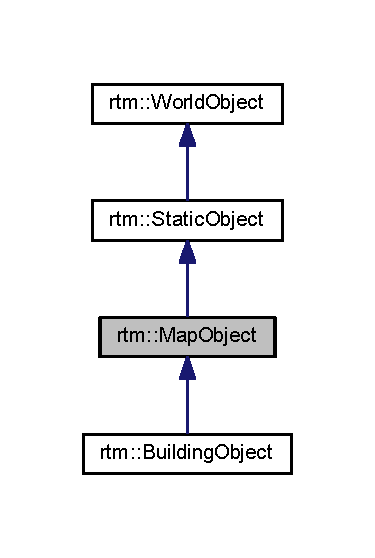
\includegraphics[width=180pt]{classrtm_1_1_map_object__inherit__graph}
\end{center}
\end{figure}
\subsection*{Открытые члены}
\begin{DoxyCompactItemize}
\item 
\mbox{\Hypertarget{classrtm_1_1_map_object_a5a739a68e3ff7439f083a998a7760287}\label{classrtm_1_1_map_object_a5a739a68e3ff7439f083a998a7760287}} 
\hyperlink{classrtm_1_1_map_object_a5a739a68e3ff7439f083a998a7760287}{Map\+Object} ()
\begin{DoxyCompactList}\small\item\em Конструктор по умочанию \end{DoxyCompactList}\item 
\hyperlink{classrtm_1_1_map_object_a39e9366932d38519d7358f74ebee9fa4}{Map\+Object} (cocos2d\+::\+Sprite $\ast$sprite, int column, int row, float angle)
\item 
\hyperlink{classrtm_1_1_map_object_ae4fbfe3193009e9e92140dc946a31bcc}{Map\+Object} (std\+::string const \&filename, int column, int row, float angle)
\item 
\mbox{\Hypertarget{classrtm_1_1_map_object_ae54a583ef69280a7b813f370979bd1b7}\label{classrtm_1_1_map_object_ae54a583ef69280a7b813f370979bd1b7}} 
virtual \hyperlink{classrtm_1_1_map_object_ae54a583ef69280a7b813f370979bd1b7}{$\sim$\+Map\+Object} ()=default
\begin{DoxyCompactList}\small\item\em Деструктор по умолчанию \end{DoxyCompactList}\end{DoxyCompactItemize}
\subsection*{Дополнительные унаследованные члены}


\subsection{Подробное описание}
Класс статического объекта карты 

\subsection{Конструктор(ы)}
\mbox{\Hypertarget{classrtm_1_1_map_object_a39e9366932d38519d7358f74ebee9fa4}\label{classrtm_1_1_map_object_a39e9366932d38519d7358f74ebee9fa4}} 
\index{rtm\+::\+Map\+Object@{rtm\+::\+Map\+Object}!Map\+Object@{Map\+Object}}
\index{Map\+Object@{Map\+Object}!rtm\+::\+Map\+Object@{rtm\+::\+Map\+Object}}
\subsubsection{\texorpdfstring{Map\+Object()}{MapObject()}\hspace{0.1cm}{\footnotesize\ttfamily [1/2]}}
{\footnotesize\ttfamily rtm\+::\+Map\+Object\+::\+Map\+Object (\begin{DoxyParamCaption}\item[{cocos2d\+::\+Sprite $\ast$}]{sprite,  }\item[{int}]{column,  }\item[{int}]{row,  }\item[{float}]{angle }\end{DoxyParamCaption})}

Конструктор с использованием уже готового спрайта 
\begin{DoxyParams}{Аргументы}
{\em sprite} & указатель на готовый спрайт \\
\hline
{\em column} & колонка, в которой необходимо отрисовать объект \\
\hline
{\em row} & строка, в которой необходимо отрисовать объект \\
\hline
{\em angle} & угол поворота объекта \\
\hline
\end{DoxyParams}
\mbox{\Hypertarget{classrtm_1_1_map_object_ae4fbfe3193009e9e92140dc946a31bcc}\label{classrtm_1_1_map_object_ae4fbfe3193009e9e92140dc946a31bcc}} 
\index{rtm\+::\+Map\+Object@{rtm\+::\+Map\+Object}!Map\+Object@{Map\+Object}}
\index{Map\+Object@{Map\+Object}!rtm\+::\+Map\+Object@{rtm\+::\+Map\+Object}}
\subsubsection{\texorpdfstring{Map\+Object()}{MapObject()}\hspace{0.1cm}{\footnotesize\ttfamily [2/2]}}
{\footnotesize\ttfamily rtm\+::\+Map\+Object\+::\+Map\+Object (\begin{DoxyParamCaption}\item[{std\+::string const \&}]{filename,  }\item[{int}]{column,  }\item[{int}]{row,  }\item[{float}]{angle }\end{DoxyParamCaption})}

Конструктор из файла 
\begin{DoxyParams}{Аргументы}
{\em filename} & путь к файлу инициализации \\
\hline
{\em column} & колонка, в которой необходимо отрисовать объект \\
\hline
{\em row} & строка, в которой необходимо отрисовать объект \\
\hline
{\em angle} & угол поворота объекта \\
\hline
\end{DoxyParams}


Объявления и описания членов классов находятся в файлах\+:\begin{DoxyCompactItemize}
\item 
C\+:/\+Users/\+Vladimir/\+Documents/\+Visual Studio 2017/\+Projects/\+R\+T\+M/\+Classes/Map\+Object.\+h\item 
C\+:/\+Users/\+Vladimir/\+Documents/\+Visual Studio 2017/\+Projects/\+R\+T\+M/\+Classes/Map\+Object.\+cpp\end{DoxyCompactItemize}

\hypertarget{classrtm_1_1_road_coating}{}\section{Класс rtm\+:\+:Road\+Coating}
\label{classrtm_1_1_road_coating}\index{rtm\+::\+Road\+Coating@{rtm\+::\+Road\+Coating}}


Класс, описывающий дороги  




{\ttfamily \#include $<$Road\+Coating.\+h$>$}



Граф наследования\+:rtm\+:\+:Road\+Coating\+:
\nopagebreak
\begin{figure}[H]
\begin{center}
\leavevmode
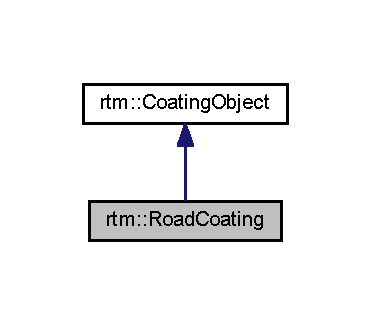
\includegraphics[width=178pt]{classrtm_1_1_road_coating__inherit__graph}
\end{center}
\end{figure}
\subsection*{Открытые члены}
\begin{DoxyCompactItemize}
\item 
\mbox{\Hypertarget{classrtm_1_1_road_coating_a0069c9e169fd982c4b5a5fa7f00145c6}\label{classrtm_1_1_road_coating_a0069c9e169fd982c4b5a5fa7f00145c6}} 
\hyperlink{classrtm_1_1_road_coating_a0069c9e169fd982c4b5a5fa7f00145c6}{Road\+Coating} ()
\begin{DoxyCompactList}\small\item\em Конструктор по умочанию \end{DoxyCompactList}\item 
\hyperlink{classrtm_1_1_road_coating_a3daed8c05e6901a8e2aedd5bd8b10e88}{Road\+Coating} (cocos2d\+::\+Sprite $\ast$const sprite, int column, int row, \hyperlink{namespacertm_a69dc82b16a0148c10962caa83d930f89}{Angle\+Type} angle, float resistance, \hyperlink{namespacertm_a4776fbfe59834ff1a16838ad6735b69a}{Directions} directions)
\item 
\hyperlink{classrtm_1_1_road_coating_ab127c8e986544a6e8bdf95ed8f302b7e}{Road\+Coating} (std\+::string const \&filename, int column, int row, \hyperlink{namespacertm_a69dc82b16a0148c10962caa83d930f89}{Angle\+Type} angle, float resistance, \hyperlink{namespacertm_a4776fbfe59834ff1a16838ad6735b69a}{Directions} directions)
\item 
\hyperlink{classrtm_1_1_road_coating_a0734f50e7884ed3cad83d0a6a16d663e}{Road\+Coating} (\hyperlink{namespacertm_aecd3929e64cd461eb3555b611f6fad95}{Coating\+Type} type, size\+\_\+t id, int column, int row, \hyperlink{namespacertm_a69dc82b16a0148c10962caa83d930f89}{Angle\+Type} angle)
\item 
\mbox{\Hypertarget{classrtm_1_1_road_coating_a49f9bc08088af98a0cccdf8db296ba0f}\label{classrtm_1_1_road_coating_a49f9bc08088af98a0cccdf8db296ba0f}} 
virtual \hyperlink{classrtm_1_1_road_coating_a49f9bc08088af98a0cccdf8db296ba0f}{$\sim$\+Road\+Coating} ()=default
\begin{DoxyCompactList}\small\item\em Деструктор по умолчанию \end{DoxyCompactList}\end{DoxyCompactItemize}
\subsection*{Закрытые статические члены}
\begin{DoxyCompactItemize}
\item 
static float \hyperlink{classrtm_1_1_road_coating_ac5bb86996945090417532dd5af056a24}{Get\+Class\+Resistance\+\_\+} (\hyperlink{namespacertm_aecd3929e64cd461eb3555b611f6fad95}{Coating\+Type} type)
\item 
static \hyperlink{namespacertm_a4776fbfe59834ff1a16838ad6735b69a}{Directions} const  \& \hyperlink{classrtm_1_1_road_coating_ae95e308d1f3998967ca420fa83f2bd93}{Get\+Class\+Directions\+\_\+} (size\+\_\+t id)
\end{DoxyCompactItemize}
\subsection*{Дополнительные унаследованные члены}


\subsection{Подробное описание}
Класс, описывающий дороги 

\subsection{Конструктор(ы)}
\mbox{\Hypertarget{classrtm_1_1_road_coating_a3daed8c05e6901a8e2aedd5bd8b10e88}\label{classrtm_1_1_road_coating_a3daed8c05e6901a8e2aedd5bd8b10e88}} 
\index{rtm\+::\+Road\+Coating@{rtm\+::\+Road\+Coating}!Road\+Coating@{Road\+Coating}}
\index{Road\+Coating@{Road\+Coating}!rtm\+::\+Road\+Coating@{rtm\+::\+Road\+Coating}}
\subsubsection{\texorpdfstring{Road\+Coating()}{RoadCoating()}\hspace{0.1cm}{\footnotesize\ttfamily [1/3]}}
{\footnotesize\ttfamily rtm\+::\+Road\+Coating\+::\+Road\+Coating (\begin{DoxyParamCaption}\item[{cocos2d\+::\+Sprite $\ast$const}]{sprite,  }\item[{int}]{column,  }\item[{int}]{row,  }\item[{\hyperlink{namespacertm_a69dc82b16a0148c10962caa83d930f89}{Angle\+Type}}]{angle,  }\item[{float}]{resistance,  }\item[{\hyperlink{namespacertm_a4776fbfe59834ff1a16838ad6735b69a}{Directions}}]{directions }\end{DoxyParamCaption})}

Конструктор с использованием уже готового спрайта 
\begin{DoxyParams}{Аргументы}
{\em sprite} & указатель на готовый спрайт \\
\hline
{\em column} & колонка, в которой необходимо отрисовать дорогу \\
\hline
{\em row} & строка, в которой необходимо отрисовать дорогу \\
\hline
{\em angle} & угол поворота дороги \\
\hline
{\em resistance} & коэффициент сопротивления на дороге \\
\hline
{\em directions} & доступные направления для движения \\
\hline
\end{DoxyParams}
\mbox{\Hypertarget{classrtm_1_1_road_coating_ab127c8e986544a6e8bdf95ed8f302b7e}\label{classrtm_1_1_road_coating_ab127c8e986544a6e8bdf95ed8f302b7e}} 
\index{rtm\+::\+Road\+Coating@{rtm\+::\+Road\+Coating}!Road\+Coating@{Road\+Coating}}
\index{Road\+Coating@{Road\+Coating}!rtm\+::\+Road\+Coating@{rtm\+::\+Road\+Coating}}
\subsubsection{\texorpdfstring{Road\+Coating()}{RoadCoating()}\hspace{0.1cm}{\footnotesize\ttfamily [2/3]}}
{\footnotesize\ttfamily rtm\+::\+Road\+Coating\+::\+Road\+Coating (\begin{DoxyParamCaption}\item[{std\+::string const \&}]{filename,  }\item[{int}]{column,  }\item[{int}]{row,  }\item[{\hyperlink{namespacertm_a69dc82b16a0148c10962caa83d930f89}{Angle\+Type}}]{angle,  }\item[{float}]{resistance,  }\item[{\hyperlink{namespacertm_a4776fbfe59834ff1a16838ad6735b69a}{Directions}}]{directions }\end{DoxyParamCaption})}

Конструктор из файла 
\begin{DoxyParams}{Аргументы}
{\em filename} & путь к файлу инициализации \\
\hline
{\em column} & колонка, в которой необходимо отрисовать дорогу \\
\hline
{\em row} & строка, в которой необходимо отрисовать дорогу \\
\hline
{\em angle} & угол поворота дороги \\
\hline
{\em resistance} & коэффициент сопротивления на дороге \\
\hline
{\em directions} & доступные направления для движения \\
\hline
\end{DoxyParams}
\mbox{\Hypertarget{classrtm_1_1_road_coating_a0734f50e7884ed3cad83d0a6a16d663e}\label{classrtm_1_1_road_coating_a0734f50e7884ed3cad83d0a6a16d663e}} 
\index{rtm\+::\+Road\+Coating@{rtm\+::\+Road\+Coating}!Road\+Coating@{Road\+Coating}}
\index{Road\+Coating@{Road\+Coating}!rtm\+::\+Road\+Coating@{rtm\+::\+Road\+Coating}}
\subsubsection{\texorpdfstring{Road\+Coating()}{RoadCoating()}\hspace{0.1cm}{\footnotesize\ttfamily [3/3]}}
{\footnotesize\ttfamily rtm\+::\+Road\+Coating\+::\+Road\+Coating (\begin{DoxyParamCaption}\item[{\hyperlink{namespacertm_aecd3929e64cd461eb3555b611f6fad95}{Coating\+Type}}]{type,  }\item[{size\+\_\+t}]{id,  }\item[{int}]{column,  }\item[{int}]{row,  }\item[{\hyperlink{namespacertm_a69dc82b16a0148c10962caa83d930f89}{Angle\+Type}}]{angle }\end{DoxyParamCaption})}

Конструктор стандартного дороги 
\begin{DoxyParams}{Аргументы}
{\em type} & стандартный тип покрытия \\
\hline
{\em id} & номер стандартной дороги \\
\hline
{\em column} & колонка, в которой необходимо отрисовать дорогу \\
\hline
{\em row} & строка, в которой необходимо отрисовать дорогу \\
\hline
{\em angle} & угол поворота дороги \\
\hline
\end{DoxyParams}


\subsection{Методы}
\mbox{\Hypertarget{classrtm_1_1_road_coating_ac5bb86996945090417532dd5af056a24}\label{classrtm_1_1_road_coating_ac5bb86996945090417532dd5af056a24}} 
\index{rtm\+::\+Road\+Coating@{rtm\+::\+Road\+Coating}!Get\+Class\+Resistance\+\_\+@{Get\+Class\+Resistance\+\_\+}}
\index{Get\+Class\+Resistance\+\_\+@{Get\+Class\+Resistance\+\_\+}!rtm\+::\+Road\+Coating@{rtm\+::\+Road\+Coating}}
\subsubsection{\texorpdfstring{Get\+Class\+Resistance\+\_\+()}{GetClassResistance\_()}}
{\footnotesize\ttfamily float rtm\+::\+Road\+Coating\+::\+Get\+Class\+Resistance\+\_\+ (\begin{DoxyParamCaption}\item[{\hyperlink{namespacertm_aecd3929e64cd461eb3555b611f6fad95}{Coating\+Type}}]{type }\end{DoxyParamCaption})\hspace{0.3cm}{\ttfamily [static]}, {\ttfamily [private]}}

Функция для получения коэффициента сопротивления на стандартной дороге по номеру 
\begin{DoxyParams}{Аргументы}
{\em type} & тип покрытия \\
\hline
\end{DoxyParams}
\begin{DoxyReturn}{Возвращает}
сопротивление 
\end{DoxyReturn}
\mbox{\Hypertarget{classrtm_1_1_road_coating_ae95e308d1f3998967ca420fa83f2bd93}\label{classrtm_1_1_road_coating_ae95e308d1f3998967ca420fa83f2bd93}} 
\index{rtm\+::\+Road\+Coating@{rtm\+::\+Road\+Coating}!Get\+Class\+Directions\+\_\+@{Get\+Class\+Directions\+\_\+}}
\index{Get\+Class\+Directions\+\_\+@{Get\+Class\+Directions\+\_\+}!rtm\+::\+Road\+Coating@{rtm\+::\+Road\+Coating}}
\subsubsection{\texorpdfstring{Get\+Class\+Directions\+\_\+()}{GetClassDirections\_()}}
{\footnotesize\ttfamily \hyperlink{namespacertm_a4776fbfe59834ff1a16838ad6735b69a}{rtm\+::\+Directions} const  \& rtm\+::\+Road\+Coating\+::\+Get\+Class\+Directions\+\_\+ (\begin{DoxyParamCaption}\item[{size\+\_\+t}]{id }\end{DoxyParamCaption})\hspace{0.3cm}{\ttfamily [static]}, {\ttfamily [private]}}

Функция для получения доступных направлений стандартной дороги по номеру 
\begin{DoxyParams}{Аргументы}
{\em id} & номер стандартной дороги \\
\hline
\end{DoxyParams}
\begin{DoxyReturn}{Возвращает}
доступные направления 
\end{DoxyReturn}


Объявления и описания членов классов находятся в файлах\+:\begin{DoxyCompactItemize}
\item 
C\+:/\+Users/\+Vladimir/\+Documents/\+Visual Studio 2017/\+Projects/\+R\+T\+M/\+Classes/Road\+Coating.\+h\item 
C\+:/\+Users/\+Vladimir/\+Documents/\+Visual Studio 2017/\+Projects/\+R\+T\+M/\+Classes/Road\+Coating.\+cpp\end{DoxyCompactItemize}

\hypertarget{structrtm_1_1_spawn_type}{}\section{Структура rtm\+:\+:Spawn\+Type}
\label{structrtm_1_1_spawn_type}\index{rtm\+::\+Spawn\+Type@{rtm\+::\+Spawn\+Type}}


Структура, описывающая параметры точки генерации объектов  




{\ttfamily \#include $<$General.\+h$>$}

\subsection*{Открытые атрибуты}
\begin{DoxyCompactItemize}
\item 
\mbox{\Hypertarget{structrtm_1_1_spawn_type_a0759515d2a862efac57fa838d706cc6f}\label{structrtm_1_1_spawn_type_a0759515d2a862efac57fa838d706cc6f}} 
int \hyperlink{structrtm_1_1_spawn_type_a0759515d2a862efac57fa838d706cc6f}{column}
\begin{DoxyCompactList}\small\item\em Номер столбца \end{DoxyCompactList}\item 
\mbox{\Hypertarget{structrtm_1_1_spawn_type_a098608b3e4273cbd65525acd8d8cbca1}\label{structrtm_1_1_spawn_type_a098608b3e4273cbd65525acd8d8cbca1}} 
int \hyperlink{structrtm_1_1_spawn_type_a098608b3e4273cbd65525acd8d8cbca1}{row}
\begin{DoxyCompactList}\small\item\em Номер строки \end{DoxyCompactList}\item 
\mbox{\Hypertarget{structrtm_1_1_spawn_type_ad375d97cdd10099f5e48fd8baf3b1145}\label{structrtm_1_1_spawn_type_ad375d97cdd10099f5e48fd8baf3b1145}} 
float \hyperlink{structrtm_1_1_spawn_type_ad375d97cdd10099f5e48fd8baf3b1145}{angle}
\begin{DoxyCompactList}\small\item\em Первоначальный угол для транспорта \end{DoxyCompactList}\end{DoxyCompactItemize}


\subsection{Подробное описание}
Структура, описывающая параметры точки генерации объектов 

Объявления и описания членов структуры находятся в файле\+:\begin{DoxyCompactItemize}
\item 
C\+:/\+Users/\+Vladimir/\+Documents/\+Visual Studio 2017/\+Projects/\+R\+T\+M/\+Classes/General.\+h\end{DoxyCompactItemize}

\hypertarget{classrtm_1_1_static_object}{}\section{Класс rtm\+:\+:Static\+Object}
\label{classrtm_1_1_static_object}\index{rtm\+::\+Static\+Object@{rtm\+::\+Static\+Object}}


Класс статического объекта (который не обновляется)  




{\ttfamily \#include $<$Static\+Object.\+h$>$}



Граф наследования\+:rtm\+:\+:Static\+Object\+:
\nopagebreak
\begin{figure}[H]
\begin{center}
\leavevmode
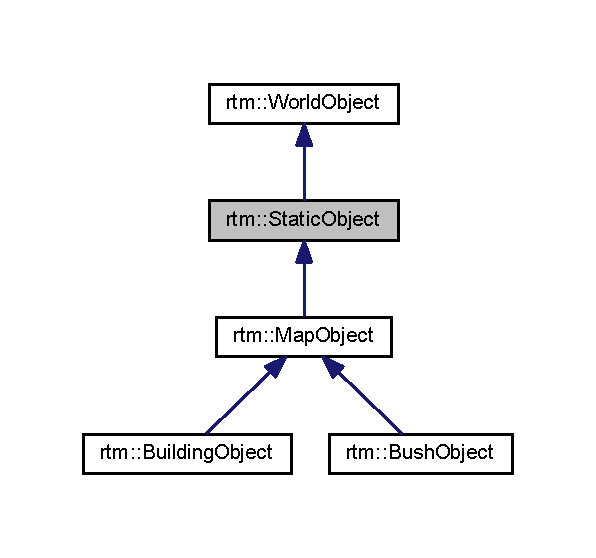
\includegraphics[width=180pt]{classrtm_1_1_static_object__inherit__graph}
\end{center}
\end{figure}
\subsection*{Открытые члены}
\begin{DoxyCompactItemize}
\item 
\mbox{\Hypertarget{classrtm_1_1_static_object_a28d0f4f8205c5ad132afca9ecfc9143e}\label{classrtm_1_1_static_object_a28d0f4f8205c5ad132afca9ecfc9143e}} 
\hyperlink{classrtm_1_1_static_object_a28d0f4f8205c5ad132afca9ecfc9143e}{Static\+Object} ()
\begin{DoxyCompactList}\small\item\em Конструктор по умочанию \end{DoxyCompactList}\item 
\hyperlink{classrtm_1_1_static_object_a98a64488b482ca02b10c0f1fed4fcad0}{Static\+Object} (cocos2d\+::\+Sprite $\ast$sprite, float x, float y, float angle)
\item 
\hyperlink{classrtm_1_1_static_object_af17012380ecde141998deadea57acd79}{Static\+Object} (std\+::string const \&filename, float x, float y, float angle)
\item 
\mbox{\Hypertarget{classrtm_1_1_static_object_ab7ae519ee89a02f8ce1178af045bdb7f}\label{classrtm_1_1_static_object_ab7ae519ee89a02f8ce1178af045bdb7f}} 
virtual \hyperlink{classrtm_1_1_static_object_ab7ae519ee89a02f8ce1178af045bdb7f}{$\sim$\+Static\+Object} ()=default
\begin{DoxyCompactList}\small\item\em Деструктор по умолчанию \end{DoxyCompactList}\end{DoxyCompactItemize}
\subsection*{Дополнительные унаследованные члены}


\subsection{Подробное описание}
Класс статического объекта (который не обновляется) 

\subsection{Конструктор(ы)}
\mbox{\Hypertarget{classrtm_1_1_static_object_a98a64488b482ca02b10c0f1fed4fcad0}\label{classrtm_1_1_static_object_a98a64488b482ca02b10c0f1fed4fcad0}} 
\index{rtm\+::\+Static\+Object@{rtm\+::\+Static\+Object}!Static\+Object@{Static\+Object}}
\index{Static\+Object@{Static\+Object}!rtm\+::\+Static\+Object@{rtm\+::\+Static\+Object}}
\subsubsection{\texorpdfstring{Static\+Object()}{StaticObject()}\hspace{0.1cm}{\footnotesize\ttfamily [1/2]}}
{\footnotesize\ttfamily rtm\+::\+Static\+Object\+::\+Static\+Object (\begin{DoxyParamCaption}\item[{cocos2d\+::\+Sprite $\ast$}]{sprite,  }\item[{float}]{x,  }\item[{float}]{y,  }\item[{float}]{angle }\end{DoxyParamCaption})}

Конструктор с использованием уже готового спрайта 
\begin{DoxyParams}{Аргументы}
{\em sprite} & указатель на готовый спрайт \\
\hline
{\em x} & абсцисса будущего объекта \\
\hline
{\em y} & ордината будущего объекта \\
\hline
{\em angle} & угол поворота строения \\
\hline
\end{DoxyParams}
\mbox{\Hypertarget{classrtm_1_1_static_object_af17012380ecde141998deadea57acd79}\label{classrtm_1_1_static_object_af17012380ecde141998deadea57acd79}} 
\index{rtm\+::\+Static\+Object@{rtm\+::\+Static\+Object}!Static\+Object@{Static\+Object}}
\index{Static\+Object@{Static\+Object}!rtm\+::\+Static\+Object@{rtm\+::\+Static\+Object}}
\subsubsection{\texorpdfstring{Static\+Object()}{StaticObject()}\hspace{0.1cm}{\footnotesize\ttfamily [2/2]}}
{\footnotesize\ttfamily rtm\+::\+Static\+Object\+::\+Static\+Object (\begin{DoxyParamCaption}\item[{std\+::string const \&}]{filename,  }\item[{float}]{x,  }\item[{float}]{y,  }\item[{float}]{angle }\end{DoxyParamCaption})}

Конструктор из файла 
\begin{DoxyParams}{Аргументы}
{\em filename} & путь к файлу инициализации \\
\hline
{\em x} & абсцисса будущего объекта \\
\hline
{\em y} & ордината будущего объекта \\
\hline
{\em angle} & угол поворота строения \\
\hline
\end{DoxyParams}


Объявления и описания членов классов находятся в файлах\+:\begin{DoxyCompactItemize}
\item 
C\+:/\+Users/\+Vladimir/\+Documents/\+Visual Studio 2017/\+Projects/\+R\+T\+M/\+Classes/Static\+Object.\+h\item 
C\+:/\+Users/\+Vladimir/\+Documents/\+Visual Studio 2017/\+Projects/\+R\+T\+M/\+Classes/Static\+Object.\+cpp\end{DoxyCompactItemize}

\hypertarget{classrtm_1_1_turn_object}{}\section{Класс rtm\+:\+:Turn\+Object}
\label{classrtm_1_1_turn_object}\index{rtm\+::\+Turn\+Object@{rtm\+::\+Turn\+Object}}


Класс поворота дороги  




{\ttfamily \#include $<$Turn\+Object.\+h$>$}



Граф наследования\+:rtm\+:\+:Turn\+Object\+:
\nopagebreak
\begin{figure}[H]
\begin{center}
\leavevmode
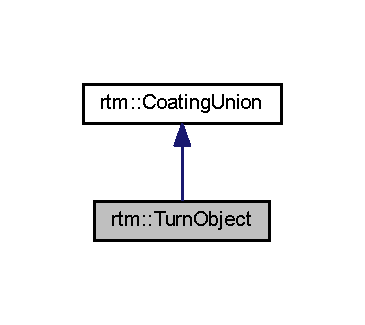
\includegraphics[width=175pt]{classrtm_1_1_turn_object__inherit__graph}
\end{center}
\end{figure}
\subsection*{Открытые члены}
\begin{DoxyCompactItemize}
\item 
\mbox{\Hypertarget{classrtm_1_1_turn_object_a987baa86c69edf1f23d1fcb2d3140ca9}\label{classrtm_1_1_turn_object_a987baa86c69edf1f23d1fcb2d3140ca9}} 
\hyperlink{classrtm_1_1_turn_object_a987baa86c69edf1f23d1fcb2d3140ca9}{Turn\+Object} ()
\begin{DoxyCompactList}\small\item\em Конструктор по умолчанию \end{DoxyCompactList}\item 
\hyperlink{classrtm_1_1_turn_object_ac673c94a34ee6dd7ece82a41fb8f7930}{Turn\+Object} (bool is\+Right, \hyperlink{namespacertm_aecd3929e64cd461eb3555b611f6fad95}{Coating\+Type} type, int column, int row, size\+\_\+t lines\+Count, \hyperlink{namespacertm_a69dc82b16a0148c10962caa83d930f89}{Angle\+Type} angle)
\begin{DoxyCompactList}\small\item\em Конструктор по размерам \end{DoxyCompactList}\item 
\mbox{\Hypertarget{classrtm_1_1_turn_object_a50ff1135e100a02294bb433ffd0a7dc6}\label{classrtm_1_1_turn_object_a50ff1135e100a02294bb433ffd0a7dc6}} 
virtual \hyperlink{classrtm_1_1_turn_object_a50ff1135e100a02294bb433ffd0a7dc6}{$\sim$\+Turn\+Object} ()=default
\begin{DoxyCompactList}\small\item\em Деструктор по умолчанию \end{DoxyCompactList}\item 
bool \hyperlink{classrtm_1_1_turn_object_ab2958c0a469d4835751b304e2bd16084}{Is\+Right} () const
\begin{DoxyCompactList}\small\item\em Функция для получения типа поворота \end{DoxyCompactList}\item 
\hyperlink{namespacertm_a69dc82b16a0148c10962caa83d930f89}{Angle\+Type} \hyperlink{classrtm_1_1_turn_object_ae3fbfdd8e940bbb61d3a68db236d60b5}{Get\+Angle} () const
\begin{DoxyCompactList}\small\item\em Функция для получения угла поворота объекта \end{DoxyCompactList}\end{DoxyCompactItemize}
\subsection*{Открытые статические члены}
\begin{DoxyCompactItemize}
\item 
static \hyperlink{namespacertm_ae3bb29510cfde424975be31866d2486e}{Coating\+Matrix} \hyperlink{classrtm_1_1_turn_object_a74dbdda621e1fbe6be1fe6373949bbad}{Right\+Turn\+Matrix} (\hyperlink{namespacertm_aecd3929e64cd461eb3555b611f6fad95}{Coating\+Type} type, int column, int row, size\+\_\+t lines\+Count, \hyperlink{namespacertm_a69dc82b16a0148c10962caa83d930f89}{Angle\+Type} angle)
\begin{DoxyCompactList}\small\item\em Функция для получения матрицы правого поворота \end{DoxyCompactList}\item 
static \hyperlink{namespacertm_ae3bb29510cfde424975be31866d2486e}{Coating\+Matrix} \hyperlink{classrtm_1_1_turn_object_a329c8abcba91f87b0dce98543d7448ba}{Left\+Turn\+Matrix} (\hyperlink{namespacertm_aecd3929e64cd461eb3555b611f6fad95}{Coating\+Type} type, int column, int row, size\+\_\+t lines\+Count, \hyperlink{namespacertm_a69dc82b16a0148c10962caa83d930f89}{Angle\+Type} angle)
\begin{DoxyCompactList}\small\item\em Функция для получения матрицы левого поворота \end{DoxyCompactList}\end{DoxyCompactItemize}
\subsection*{Закрытые данные}
\begin{DoxyCompactItemize}
\item 
\mbox{\Hypertarget{classrtm_1_1_turn_object_aae270ae895bdc8edc482e21e1784f042}\label{classrtm_1_1_turn_object_aae270ae895bdc8edc482e21e1784f042}} 
bool \hyperlink{classrtm_1_1_turn_object_aae270ae895bdc8edc482e21e1784f042}{is\+Right\+\_\+}
\begin{DoxyCompactList}\small\item\em Тип поворота \end{DoxyCompactList}\item 
\mbox{\Hypertarget{classrtm_1_1_turn_object_afcb2206b9201f0755281dc31fad29e50}\label{classrtm_1_1_turn_object_afcb2206b9201f0755281dc31fad29e50}} 
\hyperlink{namespacertm_a69dc82b16a0148c10962caa83d930f89}{Angle\+Type} \hyperlink{classrtm_1_1_turn_object_afcb2206b9201f0755281dc31fad29e50}{angle\+\_\+}
\begin{DoxyCompactList}\small\item\em Угол поворота объекта \end{DoxyCompactList}\end{DoxyCompactItemize}
\subsection*{Дополнительные унаследованные члены}


\subsection{Подробное описание}
Класс поворота дороги 

\subsection{Конструктор(ы)}
\mbox{\Hypertarget{classrtm_1_1_turn_object_ac673c94a34ee6dd7ece82a41fb8f7930}\label{classrtm_1_1_turn_object_ac673c94a34ee6dd7ece82a41fb8f7930}} 
\index{rtm\+::\+Turn\+Object@{rtm\+::\+Turn\+Object}!Turn\+Object@{Turn\+Object}}
\index{Turn\+Object@{Turn\+Object}!rtm\+::\+Turn\+Object@{rtm\+::\+Turn\+Object}}
\subsubsection{\texorpdfstring{Turn\+Object()}{TurnObject()}}
{\footnotesize\ttfamily rtm\+::\+Turn\+Object\+::\+Turn\+Object (\begin{DoxyParamCaption}\item[{bool}]{is\+Right,  }\item[{\hyperlink{namespacertm_aecd3929e64cd461eb3555b611f6fad95}{Coating\+Type}}]{type,  }\item[{int}]{column,  }\item[{int}]{row,  }\item[{size\+\_\+t}]{lines\+Count,  }\item[{\hyperlink{namespacertm_a69dc82b16a0148c10962caa83d930f89}{Angle\+Type}}]{angle }\end{DoxyParamCaption})}



Конструктор по размерам 


\begin{DoxyParams}{Аргументы}
{\em is\+Right} & тип поворота (false -\/ левый, true -\/ правый) \\
\hline
{\em type} & тип покрытия \\
\hline
{\em column} & левая колонка объекта \\
\hline
{\em row} & нижняя строка объекта \\
\hline
{\em lines\+Count} & количество полос \\
\hline
{\em angle} & угол поворота объекта \\
\hline
\end{DoxyParams}


\subsection{Методы}
\mbox{\Hypertarget{classrtm_1_1_turn_object_a74dbdda621e1fbe6be1fe6373949bbad}\label{classrtm_1_1_turn_object_a74dbdda621e1fbe6be1fe6373949bbad}} 
\index{rtm\+::\+Turn\+Object@{rtm\+::\+Turn\+Object}!Right\+Turn\+Matrix@{Right\+Turn\+Matrix}}
\index{Right\+Turn\+Matrix@{Right\+Turn\+Matrix}!rtm\+::\+Turn\+Object@{rtm\+::\+Turn\+Object}}
\subsubsection{\texorpdfstring{Right\+Turn\+Matrix()}{RightTurnMatrix()}}
{\footnotesize\ttfamily \hyperlink{namespacertm_ae3bb29510cfde424975be31866d2486e}{rtm\+::\+Coating\+Matrix} rtm\+::\+Turn\+Object\+::\+Right\+Turn\+Matrix (\begin{DoxyParamCaption}\item[{\hyperlink{namespacertm_aecd3929e64cd461eb3555b611f6fad95}{Coating\+Type}}]{type,  }\item[{int}]{column,  }\item[{int}]{row,  }\item[{size\+\_\+t}]{lines\+Count,  }\item[{\hyperlink{namespacertm_a69dc82b16a0148c10962caa83d930f89}{Angle\+Type}}]{angle }\end{DoxyParamCaption})\hspace{0.3cm}{\ttfamily [static]}}



Функция для получения матрицы правого поворота 


\begin{DoxyParams}{Аргументы}
{\em type} & тип покрытия \\
\hline
{\em column} & левая колонка объекта \\
\hline
{\em row} & нижняя строка объекта \\
\hline
{\em lines\+Count} & количество полос \\
\hline
{\em angle} & угол поворота объекта \\
\hline
\end{DoxyParams}
\begin{DoxyReturn}{Возвращает}
матрица покрытий 
\end{DoxyReturn}
\mbox{\Hypertarget{classrtm_1_1_turn_object_a329c8abcba91f87b0dce98543d7448ba}\label{classrtm_1_1_turn_object_a329c8abcba91f87b0dce98543d7448ba}} 
\index{rtm\+::\+Turn\+Object@{rtm\+::\+Turn\+Object}!Left\+Turn\+Matrix@{Left\+Turn\+Matrix}}
\index{Left\+Turn\+Matrix@{Left\+Turn\+Matrix}!rtm\+::\+Turn\+Object@{rtm\+::\+Turn\+Object}}
\subsubsection{\texorpdfstring{Left\+Turn\+Matrix()}{LeftTurnMatrix()}}
{\footnotesize\ttfamily \hyperlink{namespacertm_ae3bb29510cfde424975be31866d2486e}{rtm\+::\+Coating\+Matrix} rtm\+::\+Turn\+Object\+::\+Left\+Turn\+Matrix (\begin{DoxyParamCaption}\item[{\hyperlink{namespacertm_aecd3929e64cd461eb3555b611f6fad95}{Coating\+Type}}]{type,  }\item[{int}]{column,  }\item[{int}]{row,  }\item[{size\+\_\+t}]{lines\+Count,  }\item[{\hyperlink{namespacertm_a69dc82b16a0148c10962caa83d930f89}{Angle\+Type}}]{angle }\end{DoxyParamCaption})\hspace{0.3cm}{\ttfamily [static]}}



Функция для получения матрицы левого поворота 


\begin{DoxyParams}{Аргументы}
{\em type} & тип покрытия \\
\hline
{\em column} & левая колонка объекта \\
\hline
{\em row} & нижняя строка объекта \\
\hline
{\em lines\+Count} & количество полос \\
\hline
{\em angle} & угол поворота объекта \\
\hline
\end{DoxyParams}
\begin{DoxyReturn}{Возвращает}
матрица покрытий 
\end{DoxyReturn}
\mbox{\Hypertarget{classrtm_1_1_turn_object_ab2958c0a469d4835751b304e2bd16084}\label{classrtm_1_1_turn_object_ab2958c0a469d4835751b304e2bd16084}} 
\index{rtm\+::\+Turn\+Object@{rtm\+::\+Turn\+Object}!Is\+Right@{Is\+Right}}
\index{Is\+Right@{Is\+Right}!rtm\+::\+Turn\+Object@{rtm\+::\+Turn\+Object}}
\subsubsection{\texorpdfstring{Is\+Right()}{IsRight()}}
{\footnotesize\ttfamily bool rtm\+::\+Turn\+Object\+::\+Is\+Right (\begin{DoxyParamCaption}{ }\end{DoxyParamCaption}) const}



Функция для получения типа поворота 

\begin{DoxyReturn}{Возвращает}
true, если правый поворот, false, если левый 
\end{DoxyReturn}
\mbox{\Hypertarget{classrtm_1_1_turn_object_ae3fbfdd8e940bbb61d3a68db236d60b5}\label{classrtm_1_1_turn_object_ae3fbfdd8e940bbb61d3a68db236d60b5}} 
\index{rtm\+::\+Turn\+Object@{rtm\+::\+Turn\+Object}!Get\+Angle@{Get\+Angle}}
\index{Get\+Angle@{Get\+Angle}!rtm\+::\+Turn\+Object@{rtm\+::\+Turn\+Object}}
\subsubsection{\texorpdfstring{Get\+Angle()}{GetAngle()}}
{\footnotesize\ttfamily \hyperlink{namespacertm_a69dc82b16a0148c10962caa83d930f89}{rtm\+::\+Angle\+Type} rtm\+::\+Turn\+Object\+::\+Get\+Angle (\begin{DoxyParamCaption}{ }\end{DoxyParamCaption}) const}



Функция для получения угла поворота объекта 

\begin{DoxyReturn}{Возвращает}
угол поворота объекта 
\end{DoxyReturn}


Объявления и описания членов классов находятся в файлах\+:\begin{DoxyCompactItemize}
\item 
C\+:/\+Users/\+Vladimir/\+Documents/\+Visual Studio 2017/\+Projects/\+R\+T\+M/\+Classes/Turn\+Object.\+h\item 
C\+:/\+Users/\+Vladimir/\+Documents/\+Visual Studio 2017/\+Projects/\+R\+T\+M/\+Classes/Turn\+Object.\+cpp\end{DoxyCompactItemize}

\hypertarget{classrtm_1_1_vehicle_object}{}\section{Класс rtm\+:\+:Vehicle\+Object}
\label{classrtm_1_1_vehicle_object}\index{rtm\+::\+Vehicle\+Object@{rtm\+::\+Vehicle\+Object}}


Класс транспорта (динамического объекта карты)  




{\ttfamily \#include $<$Vehicle\+Object.\+h$>$}



Граф наследования\+:rtm\+:\+:Vehicle\+Object\+:
\nopagebreak
\begin{figure}[H]
\begin{center}
\leavevmode
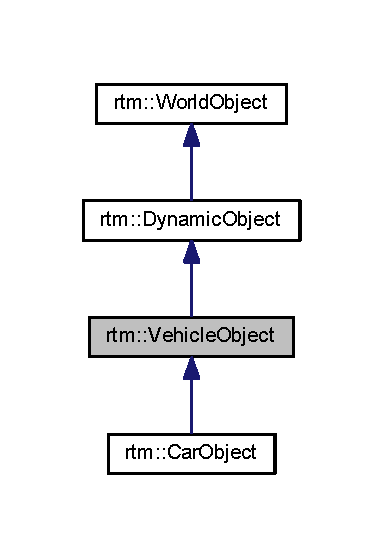
\includegraphics[width=184pt]{classrtm_1_1_vehicle_object__inherit__graph}
\end{center}
\end{figure}
\subsection*{Открытые члены}
\begin{DoxyCompactItemize}
\item 
\mbox{\Hypertarget{classrtm_1_1_vehicle_object_a11e3aa43d731f461ed503fb26c48ea5c}\label{classrtm_1_1_vehicle_object_a11e3aa43d731f461ed503fb26c48ea5c}} 
\hyperlink{classrtm_1_1_vehicle_object_a11e3aa43d731f461ed503fb26c48ea5c}{Vehicle\+Object} ()
\begin{DoxyCompactList}\small\item\em Конструктор по умочанию \end{DoxyCompactList}\item 
\hyperlink{classrtm_1_1_vehicle_object_aa14dd490d0828a12ab1e8f32bab4c98b}{Vehicle\+Object} (cocos2d\+::\+Sprite $\ast$const sprite, int column, int row, float angle, float max\+Speed, float acceleration, float deceleration)
\begin{DoxyCompactList}\small\item\em Конструктор с использованием уже готового спрайта \end{DoxyCompactList}\item 
\hyperlink{classrtm_1_1_vehicle_object_aee37c55d41eb445704b51f24cb7865cb}{Vehicle\+Object} (std\+::string const \&filename, int column, int row, float angle, float max\+Speed, float acceleration, float deceleration)
\begin{DoxyCompactList}\small\item\em Конструктор из файла \end{DoxyCompactList}\item 
\mbox{\Hypertarget{classrtm_1_1_vehicle_object_a06fe20ebdc790885520022d7f59868c0}\label{classrtm_1_1_vehicle_object_a06fe20ebdc790885520022d7f59868c0}} 
virtual \hyperlink{classrtm_1_1_vehicle_object_a06fe20ebdc790885520022d7f59868c0}{$\sim$\+Vehicle\+Object} ()=default
\begin{DoxyCompactList}\small\item\em Деструктор по умолчанию \end{DoxyCompactList}\item 
virtual void \hyperlink{classrtm_1_1_vehicle_object_a1e089c8acf528660417a21c75658d546}{Update} (\hyperlink{classrtm_1_1_world_controller}{World\+Controller} $\ast$const world) override
\begin{DoxyCompactList}\small\item\em Функция обновления \end{DoxyCompactList}\end{DoxyCompactItemize}
\subsection*{Защищенные члены}
\begin{DoxyCompactItemize}
\item 
bool \hyperlink{classrtm_1_1_vehicle_object_a017a765353387080952f3ef1657c9463}{Move\+Forward\+\_\+} ()
\begin{DoxyCompactList}\small\item\em Функция для сообщения о необходимости начать движение \end{DoxyCompactList}\item 
bool \hyperlink{classrtm_1_1_vehicle_object_a74dd5fb7b16da79e1d288738ba43ded0}{Stop\+\_\+} ()
\begin{DoxyCompactList}\small\item\em Функция для сообщения о необходимости остановиться \end{DoxyCompactList}\item 
bool \hyperlink{classrtm_1_1_vehicle_object_a0739284311dc651679c0c5954f240758}{Rotate\+\_\+} (float angle=\hyperlink{namespacertm_a39212dd73aa5a6387211cf776bdb64d8}{A\+N\+G\+L\+E\+\_\+\+R\+I\+G\+HT})
\begin{DoxyCompactList}\small\item\em Функция для сообщения о необходимости повернуть \end{DoxyCompactList}\item 
bool \hyperlink{classrtm_1_1_vehicle_object_a73ef7c4f1318bdbe2cd75dc4f07aca4e}{Change\+Line\+\_\+} (bool is\+Right=\hyperlink{namespacertm_a92d29773a54951290dd89f754fb39a8c}{L\+E\+FT})
\begin{DoxyCompactList}\small\item\em Функция для сообщения о необходимости перестроиться \end{DoxyCompactList}\item 
bool \hyperlink{classrtm_1_1_vehicle_object_adcccb796e4b1b404a25512fa8491cd43}{Is\+Movement\+\_\+} () const
\begin{DoxyCompactList}\small\item\em Функция, сообщающая о движении объекта \end{DoxyCompactList}\item 
bool \hyperlink{classrtm_1_1_vehicle_object_a7cb07a20e09d1460ec3d2dd70d62aba2}{Is\+Rotation\+\_\+} () const
\begin{DoxyCompactList}\small\item\em Функция, сообщающая о повороте объекта \end{DoxyCompactList}\item 
bool \hyperlink{classrtm_1_1_vehicle_object_a464c8de22beb3cbf819d12ad36ae4974}{Is\+Line\+Changing\+\_\+} () const
\begin{DoxyCompactList}\small\item\em Функция, сообщающая о перестроении объекта \end{DoxyCompactList}\item 
bool \hyperlink{classrtm_1_1_vehicle_object_ab74eb10fd7df8238a437923cbf184bca}{Is\+Braking\+\_\+} () const
\begin{DoxyCompactList}\small\item\em Функция, сообщающая о торможении объекта перед светофором и т.\+д. \end{DoxyCompactList}\item 
float \hyperlink{classrtm_1_1_vehicle_object_ad0dd345b8c1d7913034aaf3267ee4a03}{Get\+Max\+Speed\+\_\+} () const
\begin{DoxyCompactList}\small\item\em Функция для получения максимальной скорости \end{DoxyCompactList}\item 
float \hyperlink{classrtm_1_1_vehicle_object_a6cf4eb12c1eaf80b7f1e95ab206deae9}{Get\+Final\+Speed\+\_\+} () const
\begin{DoxyCompactList}\small\item\em Функция для получения финальной скорости (к которой объект будет стремиться) \end{DoxyCompactList}\item 
void \hyperlink{classrtm_1_1_vehicle_object_a0339478b106ebe22b63a6d076204cc22}{Set\+Final\+Speed\+\_\+} (float speed)
\begin{DoxyCompactList}\small\item\em Функция для установки финальной скорости (к которой объект будет стремиться) \end{DoxyCompactList}\item 
void \hyperlink{classrtm_1_1_vehicle_object_a3c2db832bf74ea5bd226e98e24b3da4b}{Set\+Braking\+Factor\+\_\+} (float factor)
\begin{DoxyCompactList}\small\item\em Функция для установки коэффициента торможения \end{DoxyCompactList}\item 
void \hyperlink{classrtm_1_1_vehicle_object_a124909b0d2443d501d9b1eb8d359ad5a}{Stop\+At\+Distance\+\_\+} (float distance)
\begin{DoxyCompactList}\small\item\em Функция для установки тормозого пути (объект будет пытаться остановиться за данную дистанцию) \end{DoxyCompactList}\end{DoxyCompactItemize}
\begin{Indent}\textbf{ Зрение у машин}\par
{\em Функции для просмотра окружающего мира }\begin{DoxyCompactItemize}
\item 
\hyperlink{classrtm_1_1_coating_object}{Coating\+Object} $\ast$ \hyperlink{classrtm_1_1_vehicle_object_a3756c9823f032ce8647343291fdbd00b}{Check\+Forward\+Coating\+\_\+} (\hyperlink{classrtm_1_1_world_controller}{World\+Controller} $\ast$const world, int delta=1)
\begin{DoxyCompactList}\small\item\em Функция для получения следующего по ходу движения покрытия \end{DoxyCompactList}\item 
\hyperlink{classrtm_1_1_coating_union}{Coating\+Union} $\ast$ \hyperlink{classrtm_1_1_vehicle_object_a96e80f98cc6aa50ab3f822e06223e345}{Check\+Forward\+Coating\+Union\+\_\+} (\hyperlink{classrtm_1_1_world_controller}{World\+Controller} $\ast$const world, int delta=1)
\begin{DoxyCompactList}\small\item\em Функция для получения следующего по ходу движения объединения покрытий \end{DoxyCompactList}\item 
\hyperlink{classrtm_1_1_dynamic_object}{Dynamic\+Object} $\ast$ \hyperlink{classrtm_1_1_vehicle_object_a2bc87b24a74b9eefc4e63d6618052c33}{Check\+Forward\+Area\+\_\+} (\hyperlink{classrtm_1_1_world_controller}{World\+Controller} $\ast$const world, float radius, float angle, float angle\+Shift)
\begin{DoxyCompactList}\small\item\em Функция для проверки области видимости спереди \end{DoxyCompactList}\item 
\hyperlink{classrtm_1_1_dynamic_object}{Dynamic\+Object} $\ast$ \hyperlink{classrtm_1_1_vehicle_object_a1c0c4467498e3b4a2d78c465a03fd32a}{Check\+Moving\+Area\+\_\+} (\hyperlink{classrtm_1_1_world_controller}{World\+Controller} $\ast$const world)
\begin{DoxyCompactList}\small\item\em Функция для проверки области видимости во время движения по прямой \end{DoxyCompactList}\item 
\hyperlink{classrtm_1_1_dynamic_object}{Dynamic\+Object} $\ast$ \hyperlink{classrtm_1_1_vehicle_object_a02526acf80a7bdf23f0b448a2f8b3e24}{Check\+Turn\+Area\+\_\+} (\hyperlink{classrtm_1_1_world_controller}{World\+Controller} $\ast$const world, bool is\+Right)
\begin{DoxyCompactList}\small\item\em Функция для проверки области видимости перед поворотом \end{DoxyCompactList}\item 
\hyperlink{classrtm_1_1_dynamic_object}{Dynamic\+Object} $\ast$ \hyperlink{classrtm_1_1_vehicle_object_a377af8433f7cd5cf99d8ab432dbc4e44}{Check\+Rotation\+Area\+\_\+} (\hyperlink{classrtm_1_1_world_controller}{World\+Controller} $\ast$const world)
\begin{DoxyCompactList}\small\item\em Функция для проверки области видимости во время поворота \end{DoxyCompactList}\item 
\hyperlink{classrtm_1_1_dynamic_object}{Dynamic\+Object} $\ast$ \hyperlink{classrtm_1_1_vehicle_object_a1e193bc81dc4b6c14d29c6be17db1071}{Check\+Crossroad\+Area\+\_\+} (\hyperlink{classrtm_1_1_world_controller}{World\+Controller} $\ast$const world)
\begin{DoxyCompactList}\small\item\em Функция для проверки области видимости перед нерегулируемым перекрестком \end{DoxyCompactList}\item 
\hyperlink{classrtm_1_1_dynamic_object}{Dynamic\+Object} $\ast$ \hyperlink{classrtm_1_1_vehicle_object_a397b0e3055f0dfe3f2b1b731cd5e2eb1}{Check\+Line\+Changing\+Area\+\_\+} (\hyperlink{classrtm_1_1_world_controller}{World\+Controller} $\ast$const world)
\begin{DoxyCompactList}\small\item\em Функция для проверки области видимости перед перестроением \end{DoxyCompactList}\end{DoxyCompactItemize}
\end{Indent}
\begin{Indent}\textbf{ Маневры}\par
{\em Функции выполняющиеся во время маневров }\begin{DoxyCompactItemize}
\item 
virtual void \hyperlink{classrtm_1_1_vehicle_object_abac2e84c7d102e9170843efd80c53fd2}{Before\+Moving\+\_\+} (\hyperlink{classrtm_1_1_world_controller}{World\+Controller} $\ast$const world)
\begin{DoxyCompactList}\small\item\em Функция, выполняющаяся непосредственно перед перемещением объекта \end{DoxyCompactList}\item 
virtual void \hyperlink{classrtm_1_1_vehicle_object_a4ffe184361efac31e9a009cfc4e07a1b}{After\+Moving\+\_\+} (\hyperlink{classrtm_1_1_world_controller}{World\+Controller} $\ast$const world)
\begin{DoxyCompactList}\small\item\em Функция, выполняющаяся непосредственно после перемещением объекта \end{DoxyCompactList}\item 
virtual bool \hyperlink{classrtm_1_1_vehicle_object_aa02e0b8f3fa159939f370938e45abf88}{Movement\+Start\+\_\+} (\hyperlink{classrtm_1_1_world_controller}{World\+Controller} $\ast$const world)
\begin{DoxyCompactList}\small\item\em Функция, выполняющаяся перед началом движения \end{DoxyCompactList}\item 
virtual bool \hyperlink{classrtm_1_1_vehicle_object_a06a920b3fe0df4fa4ca0687a9366426a}{Movement\+Tick\+\_\+} (\hyperlink{classrtm_1_1_world_controller}{World\+Controller} $\ast$const world)
\begin{DoxyCompactList}\small\item\em Функция, выполняющаяся во время движения \end{DoxyCompactList}\item 
virtual bool \hyperlink{classrtm_1_1_vehicle_object_a7e6c94902d1d544006ca8de63ba36860}{Movement\+End\+\_\+} (\hyperlink{classrtm_1_1_world_controller}{World\+Controller} $\ast$const world)
\begin{DoxyCompactList}\small\item\em Функция, выполняющаяся после движения (перед началом остановки) \end{DoxyCompactList}\item 
virtual bool \hyperlink{classrtm_1_1_vehicle_object_a2c449bdf4d8e954fe7bd06de4b64deb7}{Rotation\+Start\+\_\+} (\hyperlink{classrtm_1_1_world_controller}{World\+Controller} $\ast$const world)
\begin{DoxyCompactList}\small\item\em Функция, выполняющаяся перед поворотом \end{DoxyCompactList}\item 
virtual bool \hyperlink{classrtm_1_1_vehicle_object_a3dd8736f34c5e5ba26259335193628e5}{Rotation\+Tick\+\_\+} (\hyperlink{classrtm_1_1_world_controller}{World\+Controller} $\ast$const world)
\begin{DoxyCompactList}\small\item\em Функция, выполняющаяся во время поворота \end{DoxyCompactList}\item 
virtual bool \hyperlink{classrtm_1_1_vehicle_object_ab109b98ab7bda9402a6197efa98e5a03}{Rotation\+End\+\_\+} (\hyperlink{classrtm_1_1_world_controller}{World\+Controller} $\ast$const world)
\begin{DoxyCompactList}\small\item\em Функция, выполняющаяся после поворота \end{DoxyCompactList}\item 
virtual bool \hyperlink{classrtm_1_1_vehicle_object_a8976be533dfa4704f7b221c79d1fce99}{Line\+Changing\+Start} (\hyperlink{classrtm_1_1_world_controller}{World\+Controller} $\ast$const world)
\begin{DoxyCompactList}\small\item\em Функция, выполняющаяся перед перестроением \end{DoxyCompactList}\item 
virtual bool \hyperlink{classrtm_1_1_vehicle_object_ad14f2e164f2105fbae0c982cec4aff9a}{Line\+Changing\+Tick\+\_\+} (\hyperlink{classrtm_1_1_world_controller}{World\+Controller} $\ast$const world)
\begin{DoxyCompactList}\small\item\em Функция, выполняющаяся во время перестроения \end{DoxyCompactList}\item 
virtual bool \hyperlink{classrtm_1_1_vehicle_object_a61c3ec3ea6a03c4c031c2b72def10c72}{Line\+Changing\+End\+\_\+} (\hyperlink{classrtm_1_1_world_controller}{World\+Controller} $\ast$const world)
\begin{DoxyCompactList}\small\item\em Функция, выполняющаяся после перестроения \end{DoxyCompactList}\end{DoxyCompactItemize}
\end{Indent}
\subsection*{Закрытые члены}
\begin{DoxyCompactItemize}
\item 
void \hyperlink{classrtm_1_1_vehicle_object_afbfb4168caaa0b61ff8cc18e0b52275c}{Line\+Changing\+\_\+} (\hyperlink{classrtm_1_1_world_controller}{World\+Controller} $\ast$const world)
\begin{DoxyCompactList}\small\item\em Функция, выполняющая различные этапы при перестроении \end{DoxyCompactList}\item 
void \hyperlink{classrtm_1_1_vehicle_object_a6961d03a7e8a805a9bd4422a8d0c1985}{Rotation\+\_\+} (\hyperlink{classrtm_1_1_world_controller}{World\+Controller} $\ast$const world)
\begin{DoxyCompactList}\small\item\em Функция, выполняющая различные этапы при повороте \end{DoxyCompactList}\item 
void \hyperlink{classrtm_1_1_vehicle_object_a0db960e75dbcb12d028b239e441ea0ed}{Movement\+\_\+} (\hyperlink{classrtm_1_1_world_controller}{World\+Controller} $\ast$const world)
\begin{DoxyCompactList}\small\item\em Функция, выполняющая различные этапы при движении \end{DoxyCompactList}\item 
void \hyperlink{classrtm_1_1_vehicle_object_aee8f792a78b9b1becf7a84c01157520b}{Speed\+Changing\+\_\+} (\hyperlink{classrtm_1_1_world_controller}{World\+Controller} $\ast$const world)
\begin{DoxyCompactList}\small\item\em Функция, выполняющая изменение скорости в зависимости от ускорения, тормозного пути и т.\+д. \end{DoxyCompactList}\item 
void \hyperlink{classrtm_1_1_vehicle_object_a76d76e5138ecb2188bb678a361ca58d7}{Smooth\+Braking\+Counter} (\hyperlink{classrtm_1_1_world_controller}{World\+Controller} $\ast$const world)
\begin{DoxyCompactList}\small\item\em Функция, выполняющая декрементирование тормозного пути (если задан) \end{DoxyCompactList}\end{DoxyCompactItemize}
\subsection*{Закрытые данные}
\begin{DoxyCompactItemize}
\item 
\mbox{\Hypertarget{classrtm_1_1_vehicle_object_a2428e286d3d4b343aa08d7511621a80e}\label{classrtm_1_1_vehicle_object_a2428e286d3d4b343aa08d7511621a80e}} 
\hyperlink{namespacertm_a11aeba1786456e9bc054ffe33b454181}{State\+Type} \hyperlink{classrtm_1_1_vehicle_object_a2428e286d3d4b343aa08d7511621a80e}{is\+Movement\+\_\+}
\begin{DoxyCompactList}\small\item\em Этап выполнения движения (стоит, движется) \end{DoxyCompactList}\item 
\mbox{\Hypertarget{classrtm_1_1_vehicle_object_a0ffcd2c459f9e9e254fceb9dbf9f92ec}\label{classrtm_1_1_vehicle_object_a0ffcd2c459f9e9e254fceb9dbf9f92ec}} 
\hyperlink{namespacertm_a11aeba1786456e9bc054ffe33b454181}{State\+Type} \hyperlink{classrtm_1_1_vehicle_object_a0ffcd2c459f9e9e254fceb9dbf9f92ec}{is\+Rotation\+\_\+}
\begin{DoxyCompactList}\small\item\em Этап выполнения поворота \end{DoxyCompactList}\item 
\mbox{\Hypertarget{classrtm_1_1_vehicle_object_a9414b0c9f1e9efb64e1a0e3d7799645d}\label{classrtm_1_1_vehicle_object_a9414b0c9f1e9efb64e1a0e3d7799645d}} 
\hyperlink{namespacertm_a11aeba1786456e9bc054ffe33b454181}{State\+Type} \hyperlink{classrtm_1_1_vehicle_object_a9414b0c9f1e9efb64e1a0e3d7799645d}{is\+Line\+Changing\+\_\+}
\begin{DoxyCompactList}\small\item\em Этап выполнения перестроения \end{DoxyCompactList}\item 
\mbox{\Hypertarget{classrtm_1_1_vehicle_object_a364a6f04fee0079d3300c8aebb3e6b05}\label{classrtm_1_1_vehicle_object_a364a6f04fee0079d3300c8aebb3e6b05}} 
float const \hyperlink{classrtm_1_1_vehicle_object_a364a6f04fee0079d3300c8aebb3e6b05}{max\+Speed\+\_\+}
\begin{DoxyCompactList}\small\item\em Максимальная скорость \end{DoxyCompactList}\item 
\mbox{\Hypertarget{classrtm_1_1_vehicle_object_a8415f32ef87c65c05046f8e02da02dd5}\label{classrtm_1_1_vehicle_object_a8415f32ef87c65c05046f8e02da02dd5}} 
float const \hyperlink{classrtm_1_1_vehicle_object_a8415f32ef87c65c05046f8e02da02dd5}{acceleration\+\_\+}
\begin{DoxyCompactList}\small\item\em Ускорение \end{DoxyCompactList}\item 
\mbox{\Hypertarget{classrtm_1_1_vehicle_object_a2c2a8e9df92422f085eed51c446cebd2}\label{classrtm_1_1_vehicle_object_a2c2a8e9df92422f085eed51c446cebd2}} 
float const \hyperlink{classrtm_1_1_vehicle_object_a2c2a8e9df92422f085eed51c446cebd2}{deceleration\+\_\+}
\begin{DoxyCompactList}\small\item\em Скорость замедления \end{DoxyCompactList}\item 
\mbox{\Hypertarget{classrtm_1_1_vehicle_object_ac9c696fd2df6a84e3dbfad964f434641}\label{classrtm_1_1_vehicle_object_ac9c696fd2df6a84e3dbfad964f434641}} 
float \hyperlink{classrtm_1_1_vehicle_object_ac9c696fd2df6a84e3dbfad964f434641}{final\+Speed\+\_\+}
\begin{DoxyCompactList}\small\item\em Финальная скорость \end{DoxyCompactList}\item 
\mbox{\Hypertarget{classrtm_1_1_vehicle_object_a47c0ab82e158a3336f2f771b2107e9a6}\label{classrtm_1_1_vehicle_object_a47c0ab82e158a3336f2f771b2107e9a6}} 
float \hyperlink{classrtm_1_1_vehicle_object_a47c0ab82e158a3336f2f771b2107e9a6}{braking\+Factor\+\_\+}
\begin{DoxyCompactList}\small\item\em Коэффициент торможения \end{DoxyCompactList}\item 
\mbox{\Hypertarget{classrtm_1_1_vehicle_object_abe08fb06427e5ab242f46decda8cc93e}\label{classrtm_1_1_vehicle_object_abe08fb06427e5ab242f46decda8cc93e}} 
float \hyperlink{classrtm_1_1_vehicle_object_abe08fb06427e5ab242f46decda8cc93e}{braking\+Distance\+\_\+}
\begin{DoxyCompactList}\small\item\em Тормозной путь \end{DoxyCompactList}\item 
\mbox{\Hypertarget{classrtm_1_1_vehicle_object_a3382d23ebb5e01e0e1feff6c677f8947}\label{classrtm_1_1_vehicle_object_a3382d23ebb5e01e0e1feff6c677f8947}} 
float \hyperlink{classrtm_1_1_vehicle_object_a3382d23ebb5e01e0e1feff6c677f8947}{rotation\+Angle\+\_\+}
\begin{DoxyCompactList}\small\item\em Угол, на который надо повернуться \end{DoxyCompactList}\item 
\mbox{\Hypertarget{classrtm_1_1_vehicle_object_a1d89228e0e78c3edcc71c1196222c11f}\label{classrtm_1_1_vehicle_object_a1d89228e0e78c3edcc71c1196222c11f}} 
float \hyperlink{classrtm_1_1_vehicle_object_a1d89228e0e78c3edcc71c1196222c11f}{rotation\+Radius\+\_\+}
\begin{DoxyCompactList}\small\item\em Радиус окружности, по которой двигается объект \end{DoxyCompactList}\item 
\mbox{\Hypertarget{classrtm_1_1_vehicle_object_a79954d52d836f41f45a8c960708b6ad7}\label{classrtm_1_1_vehicle_object_a79954d52d836f41f45a8c960708b6ad7}} 
float \hyperlink{classrtm_1_1_vehicle_object_a79954d52d836f41f45a8c960708b6ad7}{remaining\+Offset\+\_\+}
\begin{DoxyCompactList}\small\item\em Оставшийся перпендикулярный движению сдвиг при перестроении \end{DoxyCompactList}\item 
\mbox{\Hypertarget{classrtm_1_1_vehicle_object_a94a0837b95aee16ec5662a1188f70c81}\label{classrtm_1_1_vehicle_object_a94a0837b95aee16ec5662a1188f70c81}} 
float \hyperlink{classrtm_1_1_vehicle_object_a94a0837b95aee16ec5662a1188f70c81}{remaining\+Offset\+Angle\+\_\+}
\begin{DoxyCompactList}\small\item\em Направление перестроения (перпендикулярно движению) \end{DoxyCompactList}\end{DoxyCompactItemize}


\subsection{Подробное описание}
Класс транспорта (динамического объекта карты) 

\subsection{Конструктор(ы)}
\mbox{\Hypertarget{classrtm_1_1_vehicle_object_aa14dd490d0828a12ab1e8f32bab4c98b}\label{classrtm_1_1_vehicle_object_aa14dd490d0828a12ab1e8f32bab4c98b}} 
\index{rtm\+::\+Vehicle\+Object@{rtm\+::\+Vehicle\+Object}!Vehicle\+Object@{Vehicle\+Object}}
\index{Vehicle\+Object@{Vehicle\+Object}!rtm\+::\+Vehicle\+Object@{rtm\+::\+Vehicle\+Object}}
\subsubsection{\texorpdfstring{Vehicle\+Object()}{VehicleObject()}\hspace{0.1cm}{\footnotesize\ttfamily [1/2]}}
{\footnotesize\ttfamily rtm\+::\+Vehicle\+Object\+::\+Vehicle\+Object (\begin{DoxyParamCaption}\item[{cocos2d\+::\+Sprite $\ast$const}]{sprite,  }\item[{int}]{column,  }\item[{int}]{row,  }\item[{float}]{angle,  }\item[{float}]{max\+Speed,  }\item[{float}]{acceleration,  }\item[{float}]{deceleration }\end{DoxyParamCaption})}



Конструктор с использованием уже готового спрайта 


\begin{DoxyParams}{Аргументы}
{\em sprite} & указатель на готовый спрайт \\
\hline
{\em column} & колонка, в которой необходимо отрисовать машину \\
\hline
{\em row} & строка, в которой необходимо отрисовать машину \\
\hline
{\em angle} & угол поворота машины \\
\hline
{\em max\+Speed} & максимальная скорость машины \\
\hline
{\em acceleration} & ускорение машины \\
\hline
{\em deceleration} & скорость замедления машины \\
\hline
\end{DoxyParams}
\mbox{\Hypertarget{classrtm_1_1_vehicle_object_aee37c55d41eb445704b51f24cb7865cb}\label{classrtm_1_1_vehicle_object_aee37c55d41eb445704b51f24cb7865cb}} 
\index{rtm\+::\+Vehicle\+Object@{rtm\+::\+Vehicle\+Object}!Vehicle\+Object@{Vehicle\+Object}}
\index{Vehicle\+Object@{Vehicle\+Object}!rtm\+::\+Vehicle\+Object@{rtm\+::\+Vehicle\+Object}}
\subsubsection{\texorpdfstring{Vehicle\+Object()}{VehicleObject()}\hspace{0.1cm}{\footnotesize\ttfamily [2/2]}}
{\footnotesize\ttfamily rtm\+::\+Vehicle\+Object\+::\+Vehicle\+Object (\begin{DoxyParamCaption}\item[{std\+::string const \&}]{filename,  }\item[{int}]{column,  }\item[{int}]{row,  }\item[{float}]{angle,  }\item[{float}]{max\+Speed,  }\item[{float}]{acceleration,  }\item[{float}]{deceleration }\end{DoxyParamCaption})}



Конструктор из файла 


\begin{DoxyParams}{Аргументы}
{\em filename} & путь к файлу инициализации \\
\hline
{\em column} & колонка, в которой необходимо отрисовать машину \\
\hline
{\em row} & строка, в которой необходимо отрисовать машину \\
\hline
{\em angle} & угол поворота машины \\
\hline
{\em max\+Speed} & максимальная скорость машины \\
\hline
{\em acceleration} & ускорение машины \\
\hline
{\em deceleration} & скорость замедления машины \\
\hline
\end{DoxyParams}


\subsection{Методы}
\mbox{\Hypertarget{classrtm_1_1_vehicle_object_a1e089c8acf528660417a21c75658d546}\label{classrtm_1_1_vehicle_object_a1e089c8acf528660417a21c75658d546}} 
\index{rtm\+::\+Vehicle\+Object@{rtm\+::\+Vehicle\+Object}!Update@{Update}}
\index{Update@{Update}!rtm\+::\+Vehicle\+Object@{rtm\+::\+Vehicle\+Object}}
\subsubsection{\texorpdfstring{Update()}{Update()}}
{\footnotesize\ttfamily void rtm\+::\+Vehicle\+Object\+::\+Update (\begin{DoxyParamCaption}\item[{\hyperlink{classrtm_1_1_world_controller}{World\+Controller} $\ast$const}]{world }\end{DoxyParamCaption})\hspace{0.3cm}{\ttfamily [override]}, {\ttfamily [virtual]}}



Функция обновления 


\begin{DoxyParams}{Аргументы}
{\em world} & контроллер мира, в котором находится объект \\
\hline
\end{DoxyParams}


Переопределяет метод предка \hyperlink{classrtm_1_1_dynamic_object_a2b2a4072f80d6be9c8d1097bc072197e}{rtm\+::\+Dynamic\+Object}.

\mbox{\Hypertarget{classrtm_1_1_vehicle_object_a017a765353387080952f3ef1657c9463}\label{classrtm_1_1_vehicle_object_a017a765353387080952f3ef1657c9463}} 
\index{rtm\+::\+Vehicle\+Object@{rtm\+::\+Vehicle\+Object}!Move\+Forward\+\_\+@{Move\+Forward\+\_\+}}
\index{Move\+Forward\+\_\+@{Move\+Forward\+\_\+}!rtm\+::\+Vehicle\+Object@{rtm\+::\+Vehicle\+Object}}
\subsubsection{\texorpdfstring{Move\+Forward\+\_\+()}{MoveForward\_()}}
{\footnotesize\ttfamily bool rtm\+::\+Vehicle\+Object\+::\+Move\+Forward\+\_\+ (\begin{DoxyParamCaption}{ }\end{DoxyParamCaption})\hspace{0.3cm}{\ttfamily [protected]}}



Функция для сообщения о необходимости начать движение 

\begin{DoxyReturn}{Возвращает}
true, если возможно начать движение, иначе false 
\end{DoxyReturn}
\mbox{\Hypertarget{classrtm_1_1_vehicle_object_a74dd5fb7b16da79e1d288738ba43ded0}\label{classrtm_1_1_vehicle_object_a74dd5fb7b16da79e1d288738ba43ded0}} 
\index{rtm\+::\+Vehicle\+Object@{rtm\+::\+Vehicle\+Object}!Stop\+\_\+@{Stop\+\_\+}}
\index{Stop\+\_\+@{Stop\+\_\+}!rtm\+::\+Vehicle\+Object@{rtm\+::\+Vehicle\+Object}}
\subsubsection{\texorpdfstring{Stop\+\_\+()}{Stop\_()}}
{\footnotesize\ttfamily bool rtm\+::\+Vehicle\+Object\+::\+Stop\+\_\+ (\begin{DoxyParamCaption}{ }\end{DoxyParamCaption})\hspace{0.3cm}{\ttfamily [protected]}}



Функция для сообщения о необходимости остановиться 

\begin{DoxyReturn}{Возвращает}
true, если возможно остановиться, иначе false 
\end{DoxyReturn}
\mbox{\Hypertarget{classrtm_1_1_vehicle_object_a0739284311dc651679c0c5954f240758}\label{classrtm_1_1_vehicle_object_a0739284311dc651679c0c5954f240758}} 
\index{rtm\+::\+Vehicle\+Object@{rtm\+::\+Vehicle\+Object}!Rotate\+\_\+@{Rotate\+\_\+}}
\index{Rotate\+\_\+@{Rotate\+\_\+}!rtm\+::\+Vehicle\+Object@{rtm\+::\+Vehicle\+Object}}
\subsubsection{\texorpdfstring{Rotate\+\_\+()}{Rotate\_()}}
{\footnotesize\ttfamily bool rtm\+::\+Vehicle\+Object\+::\+Rotate\+\_\+ (\begin{DoxyParamCaption}\item[{float}]{angle = {\ttfamily \hyperlink{namespacertm_a39212dd73aa5a6387211cf776bdb64d8}{A\+N\+G\+L\+E\+\_\+\+R\+I\+G\+HT}} }\end{DoxyParamCaption})\hspace{0.3cm}{\ttfamily [protected]}}



Функция для сообщения о необходимости повернуть 


\begin{DoxyParams}{Аргументы}
{\em angle} & угол, на который необходимо повернуть \\
\hline
\end{DoxyParams}
\begin{DoxyReturn}{Возвращает}
true, если возможно повернуть, иначе false (если поворот уже начат) 
\end{DoxyReturn}
\mbox{\Hypertarget{classrtm_1_1_vehicle_object_a73ef7c4f1318bdbe2cd75dc4f07aca4e}\label{classrtm_1_1_vehicle_object_a73ef7c4f1318bdbe2cd75dc4f07aca4e}} 
\index{rtm\+::\+Vehicle\+Object@{rtm\+::\+Vehicle\+Object}!Change\+Line\+\_\+@{Change\+Line\+\_\+}}
\index{Change\+Line\+\_\+@{Change\+Line\+\_\+}!rtm\+::\+Vehicle\+Object@{rtm\+::\+Vehicle\+Object}}
\subsubsection{\texorpdfstring{Change\+Line\+\_\+()}{ChangeLine\_()}}
{\footnotesize\ttfamily bool rtm\+::\+Vehicle\+Object\+::\+Change\+Line\+\_\+ (\begin{DoxyParamCaption}\item[{bool}]{is\+Right = {\ttfamily \hyperlink{namespacertm_a92d29773a54951290dd89f754fb39a8c}{L\+E\+FT}} }\end{DoxyParamCaption})\hspace{0.3cm}{\ttfamily [protected]}}



Функция для сообщения о необходимости перестроиться 


\begin{DoxyParams}{Аргументы}
{\em is\+Right} & сторона, в которую надо перестроиться (можно использовать константы \hyperlink{namespacertm_a92d29773a54951290dd89f754fb39a8c}{rtm\+::\+L\+E\+FT} и \hyperlink{namespacertm_a18eb7493925a15e12096e1a6170c3da7}{rtm\+::\+R\+I\+G\+HT}) \\
\hline
\end{DoxyParams}
\begin{DoxyReturn}{Возвращает}
true, если возможно перестроиться, иначе false 
\end{DoxyReturn}
\mbox{\Hypertarget{classrtm_1_1_vehicle_object_adcccb796e4b1b404a25512fa8491cd43}\label{classrtm_1_1_vehicle_object_adcccb796e4b1b404a25512fa8491cd43}} 
\index{rtm\+::\+Vehicle\+Object@{rtm\+::\+Vehicle\+Object}!Is\+Movement\+\_\+@{Is\+Movement\+\_\+}}
\index{Is\+Movement\+\_\+@{Is\+Movement\+\_\+}!rtm\+::\+Vehicle\+Object@{rtm\+::\+Vehicle\+Object}}
\subsubsection{\texorpdfstring{Is\+Movement\+\_\+()}{IsMovement\_()}}
{\footnotesize\ttfamily bool rtm\+::\+Vehicle\+Object\+::\+Is\+Movement\+\_\+ (\begin{DoxyParamCaption}{ }\end{DoxyParamCaption}) const\hspace{0.3cm}{\ttfamily [protected]}}



Функция, сообщающая о движении объекта 

\begin{DoxyReturn}{Возвращает}
true, если объект движется, иначе false 
\end{DoxyReturn}
\mbox{\Hypertarget{classrtm_1_1_vehicle_object_a7cb07a20e09d1460ec3d2dd70d62aba2}\label{classrtm_1_1_vehicle_object_a7cb07a20e09d1460ec3d2dd70d62aba2}} 
\index{rtm\+::\+Vehicle\+Object@{rtm\+::\+Vehicle\+Object}!Is\+Rotation\+\_\+@{Is\+Rotation\+\_\+}}
\index{Is\+Rotation\+\_\+@{Is\+Rotation\+\_\+}!rtm\+::\+Vehicle\+Object@{rtm\+::\+Vehicle\+Object}}
\subsubsection{\texorpdfstring{Is\+Rotation\+\_\+()}{IsRotation\_()}}
{\footnotesize\ttfamily bool rtm\+::\+Vehicle\+Object\+::\+Is\+Rotation\+\_\+ (\begin{DoxyParamCaption}{ }\end{DoxyParamCaption}) const\hspace{0.3cm}{\ttfamily [protected]}}



Функция, сообщающая о повороте объекта 

\begin{DoxyReturn}{Возвращает}
true, если объект поворачивает, иначе false 
\end{DoxyReturn}
\mbox{\Hypertarget{classrtm_1_1_vehicle_object_a464c8de22beb3cbf819d12ad36ae4974}\label{classrtm_1_1_vehicle_object_a464c8de22beb3cbf819d12ad36ae4974}} 
\index{rtm\+::\+Vehicle\+Object@{rtm\+::\+Vehicle\+Object}!Is\+Line\+Changing\+\_\+@{Is\+Line\+Changing\+\_\+}}
\index{Is\+Line\+Changing\+\_\+@{Is\+Line\+Changing\+\_\+}!rtm\+::\+Vehicle\+Object@{rtm\+::\+Vehicle\+Object}}
\subsubsection{\texorpdfstring{Is\+Line\+Changing\+\_\+()}{IsLineChanging\_()}}
{\footnotesize\ttfamily bool rtm\+::\+Vehicle\+Object\+::\+Is\+Line\+Changing\+\_\+ (\begin{DoxyParamCaption}{ }\end{DoxyParamCaption}) const\hspace{0.3cm}{\ttfamily [protected]}}



Функция, сообщающая о перестроении объекта 

\begin{DoxyReturn}{Возвращает}
true, если объект перестраивается, иначе false 
\end{DoxyReturn}
\mbox{\Hypertarget{classrtm_1_1_vehicle_object_ab74eb10fd7df8238a437923cbf184bca}\label{classrtm_1_1_vehicle_object_ab74eb10fd7df8238a437923cbf184bca}} 
\index{rtm\+::\+Vehicle\+Object@{rtm\+::\+Vehicle\+Object}!Is\+Braking\+\_\+@{Is\+Braking\+\_\+}}
\index{Is\+Braking\+\_\+@{Is\+Braking\+\_\+}!rtm\+::\+Vehicle\+Object@{rtm\+::\+Vehicle\+Object}}
\subsubsection{\texorpdfstring{Is\+Braking\+\_\+()}{IsBraking\_()}}
{\footnotesize\ttfamily bool rtm\+::\+Vehicle\+Object\+::\+Is\+Braking\+\_\+ (\begin{DoxyParamCaption}{ }\end{DoxyParamCaption}) const\hspace{0.3cm}{\ttfamily [protected]}}



Функция, сообщающая о торможении объекта перед светофором и т.\+д. 

\begin{DoxyReturn}{Возвращает}
true, если объект тормозит, иначе false 
\end{DoxyReturn}
\mbox{\Hypertarget{classrtm_1_1_vehicle_object_ad0dd345b8c1d7913034aaf3267ee4a03}\label{classrtm_1_1_vehicle_object_ad0dd345b8c1d7913034aaf3267ee4a03}} 
\index{rtm\+::\+Vehicle\+Object@{rtm\+::\+Vehicle\+Object}!Get\+Max\+Speed\+\_\+@{Get\+Max\+Speed\+\_\+}}
\index{Get\+Max\+Speed\+\_\+@{Get\+Max\+Speed\+\_\+}!rtm\+::\+Vehicle\+Object@{rtm\+::\+Vehicle\+Object}}
\subsubsection{\texorpdfstring{Get\+Max\+Speed\+\_\+()}{GetMaxSpeed\_()}}
{\footnotesize\ttfamily float rtm\+::\+Vehicle\+Object\+::\+Get\+Max\+Speed\+\_\+ (\begin{DoxyParamCaption}{ }\end{DoxyParamCaption}) const\hspace{0.3cm}{\ttfamily [protected]}}



Функция для получения максимальной скорости 

\begin{DoxyReturn}{Возвращает}
максимальная скорость 
\end{DoxyReturn}
\mbox{\Hypertarget{classrtm_1_1_vehicle_object_a6cf4eb12c1eaf80b7f1e95ab206deae9}\label{classrtm_1_1_vehicle_object_a6cf4eb12c1eaf80b7f1e95ab206deae9}} 
\index{rtm\+::\+Vehicle\+Object@{rtm\+::\+Vehicle\+Object}!Get\+Final\+Speed\+\_\+@{Get\+Final\+Speed\+\_\+}}
\index{Get\+Final\+Speed\+\_\+@{Get\+Final\+Speed\+\_\+}!rtm\+::\+Vehicle\+Object@{rtm\+::\+Vehicle\+Object}}
\subsubsection{\texorpdfstring{Get\+Final\+Speed\+\_\+()}{GetFinalSpeed\_()}}
{\footnotesize\ttfamily float rtm\+::\+Vehicle\+Object\+::\+Get\+Final\+Speed\+\_\+ (\begin{DoxyParamCaption}{ }\end{DoxyParamCaption}) const\hspace{0.3cm}{\ttfamily [protected]}}



Функция для получения финальной скорости (к которой объект будет стремиться) 

\begin{DoxyReturn}{Возвращает}
конечная скорость 
\end{DoxyReturn}
\mbox{\Hypertarget{classrtm_1_1_vehicle_object_a0339478b106ebe22b63a6d076204cc22}\label{classrtm_1_1_vehicle_object_a0339478b106ebe22b63a6d076204cc22}} 
\index{rtm\+::\+Vehicle\+Object@{rtm\+::\+Vehicle\+Object}!Set\+Final\+Speed\+\_\+@{Set\+Final\+Speed\+\_\+}}
\index{Set\+Final\+Speed\+\_\+@{Set\+Final\+Speed\+\_\+}!rtm\+::\+Vehicle\+Object@{rtm\+::\+Vehicle\+Object}}
\subsubsection{\texorpdfstring{Set\+Final\+Speed\+\_\+()}{SetFinalSpeed\_()}}
{\footnotesize\ttfamily void rtm\+::\+Vehicle\+Object\+::\+Set\+Final\+Speed\+\_\+ (\begin{DoxyParamCaption}\item[{float}]{speed }\end{DoxyParamCaption})\hspace{0.3cm}{\ttfamily [protected]}}



Функция для установки финальной скорости (к которой объект будет стремиться) 


\begin{DoxyParams}{Аргументы}
{\em speed} & новая скорость \\
\hline
\end{DoxyParams}
\mbox{\Hypertarget{classrtm_1_1_vehicle_object_a3c2db832bf74ea5bd226e98e24b3da4b}\label{classrtm_1_1_vehicle_object_a3c2db832bf74ea5bd226e98e24b3da4b}} 
\index{rtm\+::\+Vehicle\+Object@{rtm\+::\+Vehicle\+Object}!Set\+Braking\+Factor\+\_\+@{Set\+Braking\+Factor\+\_\+}}
\index{Set\+Braking\+Factor\+\_\+@{Set\+Braking\+Factor\+\_\+}!rtm\+::\+Vehicle\+Object@{rtm\+::\+Vehicle\+Object}}
\subsubsection{\texorpdfstring{Set\+Braking\+Factor\+\_\+()}{SetBrakingFactor\_()}}
{\footnotesize\ttfamily void rtm\+::\+Vehicle\+Object\+::\+Set\+Braking\+Factor\+\_\+ (\begin{DoxyParamCaption}\item[{float}]{factor }\end{DoxyParamCaption})\hspace{0.3cm}{\ttfamily [protected]}}



Функция для установки коэффициента торможения 


\begin{DoxyParams}{Аргументы}
{\em factor} & новый коэффициент торможения (1 -\/ торможение с обычным ускорением) \\
\hline
\end{DoxyParams}
\mbox{\Hypertarget{classrtm_1_1_vehicle_object_a124909b0d2443d501d9b1eb8d359ad5a}\label{classrtm_1_1_vehicle_object_a124909b0d2443d501d9b1eb8d359ad5a}} 
\index{rtm\+::\+Vehicle\+Object@{rtm\+::\+Vehicle\+Object}!Stop\+At\+Distance\+\_\+@{Stop\+At\+Distance\+\_\+}}
\index{Stop\+At\+Distance\+\_\+@{Stop\+At\+Distance\+\_\+}!rtm\+::\+Vehicle\+Object@{rtm\+::\+Vehicle\+Object}}
\subsubsection{\texorpdfstring{Stop\+At\+Distance\+\_\+()}{StopAtDistance\_()}}
{\footnotesize\ttfamily void rtm\+::\+Vehicle\+Object\+::\+Stop\+At\+Distance\+\_\+ (\begin{DoxyParamCaption}\item[{float}]{distance }\end{DoxyParamCaption})\hspace{0.3cm}{\ttfamily [protected]}}



Функция для установки тормозого пути (объект будет пытаться остановиться за данную дистанцию) 


\begin{DoxyParams}{Аргументы}
{\em distance} & дистанция, за которую необходимо остановиться \\
\hline
\end{DoxyParams}
\mbox{\Hypertarget{classrtm_1_1_vehicle_object_a3756c9823f032ce8647343291fdbd00b}\label{classrtm_1_1_vehicle_object_a3756c9823f032ce8647343291fdbd00b}} 
\index{rtm\+::\+Vehicle\+Object@{rtm\+::\+Vehicle\+Object}!Check\+Forward\+Coating\+\_\+@{Check\+Forward\+Coating\+\_\+}}
\index{Check\+Forward\+Coating\+\_\+@{Check\+Forward\+Coating\+\_\+}!rtm\+::\+Vehicle\+Object@{rtm\+::\+Vehicle\+Object}}
\subsubsection{\texorpdfstring{Check\+Forward\+Coating\+\_\+()}{CheckForwardCoating\_()}}
{\footnotesize\ttfamily \hyperlink{classrtm_1_1_coating_object}{rtm\+::\+Coating\+Object} $\ast$ rtm\+::\+Vehicle\+Object\+::\+Check\+Forward\+Coating\+\_\+ (\begin{DoxyParamCaption}\item[{\hyperlink{classrtm_1_1_world_controller}{World\+Controller} $\ast$const}]{world,  }\item[{int}]{delta = {\ttfamily 1} }\end{DoxyParamCaption})\hspace{0.3cm}{\ttfamily [protected]}}



Функция для получения следующего по ходу движения покрытия 


\begin{DoxyParams}{Аргументы}
{\em world} & контроллер мира, в котором находится объект \\
\hline
{\em delta} & сдвиг в клетках относительно данного объекта (1 -\/ следующая, 2 -\/ через одну) \\
\hline
\end{DoxyParams}
\begin{DoxyReturn}{Возвращает}
указатель на покрытие 
\end{DoxyReturn}
\mbox{\Hypertarget{classrtm_1_1_vehicle_object_a96e80f98cc6aa50ab3f822e06223e345}\label{classrtm_1_1_vehicle_object_a96e80f98cc6aa50ab3f822e06223e345}} 
\index{rtm\+::\+Vehicle\+Object@{rtm\+::\+Vehicle\+Object}!Check\+Forward\+Coating\+Union\+\_\+@{Check\+Forward\+Coating\+Union\+\_\+}}
\index{Check\+Forward\+Coating\+Union\+\_\+@{Check\+Forward\+Coating\+Union\+\_\+}!rtm\+::\+Vehicle\+Object@{rtm\+::\+Vehicle\+Object}}
\subsubsection{\texorpdfstring{Check\+Forward\+Coating\+Union\+\_\+()}{CheckForwardCoatingUnion\_()}}
{\footnotesize\ttfamily \hyperlink{classrtm_1_1_coating_union}{rtm\+::\+Coating\+Union} $\ast$ rtm\+::\+Vehicle\+Object\+::\+Check\+Forward\+Coating\+Union\+\_\+ (\begin{DoxyParamCaption}\item[{\hyperlink{classrtm_1_1_world_controller}{World\+Controller} $\ast$const}]{world,  }\item[{int}]{delta = {\ttfamily 1} }\end{DoxyParamCaption})\hspace{0.3cm}{\ttfamily [protected]}}



Функция для получения следующего по ходу движения объединения покрытий 


\begin{DoxyParams}{Аргументы}
{\em world} & контроллер мира, в котором находится объект \\
\hline
{\em delta} & сдвиг в клетках относительно данного объекта (1 -\/ следующее, 2 -\/ через одно) \\
\hline
\end{DoxyParams}
\begin{DoxyReturn}{Возвращает}
указатель на объединение покрытий 
\end{DoxyReturn}
\mbox{\Hypertarget{classrtm_1_1_vehicle_object_a2bc87b24a74b9eefc4e63d6618052c33}\label{classrtm_1_1_vehicle_object_a2bc87b24a74b9eefc4e63d6618052c33}} 
\index{rtm\+::\+Vehicle\+Object@{rtm\+::\+Vehicle\+Object}!Check\+Forward\+Area\+\_\+@{Check\+Forward\+Area\+\_\+}}
\index{Check\+Forward\+Area\+\_\+@{Check\+Forward\+Area\+\_\+}!rtm\+::\+Vehicle\+Object@{rtm\+::\+Vehicle\+Object}}
\subsubsection{\texorpdfstring{Check\+Forward\+Area\+\_\+()}{CheckForwardArea\_()}}
{\footnotesize\ttfamily \hyperlink{classrtm_1_1_dynamic_object}{rtm\+::\+Dynamic\+Object} $\ast$ rtm\+::\+Vehicle\+Object\+::\+Check\+Forward\+Area\+\_\+ (\begin{DoxyParamCaption}\item[{\hyperlink{classrtm_1_1_world_controller}{World\+Controller} $\ast$const}]{world,  }\item[{float}]{radius,  }\item[{float}]{angle,  }\item[{float}]{angle\+Shift }\end{DoxyParamCaption})\hspace{0.3cm}{\ttfamily [protected]}}



Функция для проверки области видимости спереди 


\begin{DoxyParams}{Аргументы}
{\em world} & контроллер мира, в котором находится данный объект \\
\hline
{\em radius} & радиус видимости \\
\hline
{\em angle} & угол видимости (в каждую из сторон) \\
\hline
{\em angle\+Shift} & сдвиг области видимости \\
\hline
\end{DoxyParams}
\begin{DoxyReturn}{Возвращает}
указатель на объект, находящийся в области видимости 

nullptr, если нет объектов в области видимости 
\end{DoxyReturn}
\mbox{\Hypertarget{classrtm_1_1_vehicle_object_a1c0c4467498e3b4a2d78c465a03fd32a}\label{classrtm_1_1_vehicle_object_a1c0c4467498e3b4a2d78c465a03fd32a}} 
\index{rtm\+::\+Vehicle\+Object@{rtm\+::\+Vehicle\+Object}!Check\+Moving\+Area\+\_\+@{Check\+Moving\+Area\+\_\+}}
\index{Check\+Moving\+Area\+\_\+@{Check\+Moving\+Area\+\_\+}!rtm\+::\+Vehicle\+Object@{rtm\+::\+Vehicle\+Object}}
\subsubsection{\texorpdfstring{Check\+Moving\+Area\+\_\+()}{CheckMovingArea\_()}}
{\footnotesize\ttfamily \hyperlink{classrtm_1_1_dynamic_object}{rtm\+::\+Dynamic\+Object} $\ast$ rtm\+::\+Vehicle\+Object\+::\+Check\+Moving\+Area\+\_\+ (\begin{DoxyParamCaption}\item[{\hyperlink{classrtm_1_1_world_controller}{World\+Controller} $\ast$const}]{world }\end{DoxyParamCaption})\hspace{0.3cm}{\ttfamily [protected]}}



Функция для проверки области видимости во время движения по прямой 


\begin{DoxyParams}{Аргументы}
{\em world} & контроллер мира, в котором находится данный объект \\
\hline
\end{DoxyParams}
\begin{DoxyReturn}{Возвращает}
указатель на объект, находящийся в области видимости 

nullptr, если нет объектов в области видимости 
\end{DoxyReturn}
\mbox{\Hypertarget{classrtm_1_1_vehicle_object_a02526acf80a7bdf23f0b448a2f8b3e24}\label{classrtm_1_1_vehicle_object_a02526acf80a7bdf23f0b448a2f8b3e24}} 
\index{rtm\+::\+Vehicle\+Object@{rtm\+::\+Vehicle\+Object}!Check\+Turn\+Area\+\_\+@{Check\+Turn\+Area\+\_\+}}
\index{Check\+Turn\+Area\+\_\+@{Check\+Turn\+Area\+\_\+}!rtm\+::\+Vehicle\+Object@{rtm\+::\+Vehicle\+Object}}
\subsubsection{\texorpdfstring{Check\+Turn\+Area\+\_\+()}{CheckTurnArea\_()}}
{\footnotesize\ttfamily \hyperlink{classrtm_1_1_dynamic_object}{rtm\+::\+Dynamic\+Object} $\ast$ rtm\+::\+Vehicle\+Object\+::\+Check\+Turn\+Area\+\_\+ (\begin{DoxyParamCaption}\item[{\hyperlink{classrtm_1_1_world_controller}{World\+Controller} $\ast$const}]{world,  }\item[{bool}]{is\+Right }\end{DoxyParamCaption})\hspace{0.3cm}{\ttfamily [protected]}}



Функция для проверки области видимости перед поворотом 


\begin{DoxyParams}{Аргументы}
{\em world} & контроллер мира, в котором находится данный объект \\
\hline
{\em is\+Right} & сторона, в которую совершается поворот (тип поворота) \\
\hline
\end{DoxyParams}
\begin{DoxyReturn}{Возвращает}
указатель на объект, находящийся в области видимости 

nullptr, если нет объектов в области видимости 
\end{DoxyReturn}
\mbox{\Hypertarget{classrtm_1_1_vehicle_object_a377af8433f7cd5cf99d8ab432dbc4e44}\label{classrtm_1_1_vehicle_object_a377af8433f7cd5cf99d8ab432dbc4e44}} 
\index{rtm\+::\+Vehicle\+Object@{rtm\+::\+Vehicle\+Object}!Check\+Rotation\+Area\+\_\+@{Check\+Rotation\+Area\+\_\+}}
\index{Check\+Rotation\+Area\+\_\+@{Check\+Rotation\+Area\+\_\+}!rtm\+::\+Vehicle\+Object@{rtm\+::\+Vehicle\+Object}}
\subsubsection{\texorpdfstring{Check\+Rotation\+Area\+\_\+()}{CheckRotationArea\_()}}
{\footnotesize\ttfamily \hyperlink{classrtm_1_1_dynamic_object}{rtm\+::\+Dynamic\+Object} $\ast$ rtm\+::\+Vehicle\+Object\+::\+Check\+Rotation\+Area\+\_\+ (\begin{DoxyParamCaption}\item[{\hyperlink{classrtm_1_1_world_controller}{World\+Controller} $\ast$const}]{world }\end{DoxyParamCaption})\hspace{0.3cm}{\ttfamily [protected]}}



Функция для проверки области видимости во время поворота 


\begin{DoxyParams}{Аргументы}
{\em world} & контроллер мира, в котором находится данный объект \\
\hline
\end{DoxyParams}
\begin{DoxyReturn}{Возвращает}
указатель на объект, находящийся в области видимости 

nullptr, если нет объектов в области видимости 
\end{DoxyReturn}
\mbox{\Hypertarget{classrtm_1_1_vehicle_object_a1e193bc81dc4b6c14d29c6be17db1071}\label{classrtm_1_1_vehicle_object_a1e193bc81dc4b6c14d29c6be17db1071}} 
\index{rtm\+::\+Vehicle\+Object@{rtm\+::\+Vehicle\+Object}!Check\+Crossroad\+Area\+\_\+@{Check\+Crossroad\+Area\+\_\+}}
\index{Check\+Crossroad\+Area\+\_\+@{Check\+Crossroad\+Area\+\_\+}!rtm\+::\+Vehicle\+Object@{rtm\+::\+Vehicle\+Object}}
\subsubsection{\texorpdfstring{Check\+Crossroad\+Area\+\_\+()}{CheckCrossroadArea\_()}}
{\footnotesize\ttfamily \hyperlink{classrtm_1_1_dynamic_object}{rtm\+::\+Dynamic\+Object} $\ast$ rtm\+::\+Vehicle\+Object\+::\+Check\+Crossroad\+Area\+\_\+ (\begin{DoxyParamCaption}\item[{\hyperlink{classrtm_1_1_world_controller}{World\+Controller} $\ast$const}]{world }\end{DoxyParamCaption})\hspace{0.3cm}{\ttfamily [protected]}}



Функция для проверки области видимости перед нерегулируемым перекрестком 


\begin{DoxyParams}{Аргументы}
{\em world} & контроллер мира, в котором находится данный объект \\
\hline
\end{DoxyParams}
\begin{DoxyReturn}{Возвращает}
указатель на объект, находящийся в области видимости 

nullptr, если нет объектов в области видимости 
\end{DoxyReturn}
\mbox{\Hypertarget{classrtm_1_1_vehicle_object_a397b0e3055f0dfe3f2b1b731cd5e2eb1}\label{classrtm_1_1_vehicle_object_a397b0e3055f0dfe3f2b1b731cd5e2eb1}} 
\index{rtm\+::\+Vehicle\+Object@{rtm\+::\+Vehicle\+Object}!Check\+Line\+Changing\+Area\+\_\+@{Check\+Line\+Changing\+Area\+\_\+}}
\index{Check\+Line\+Changing\+Area\+\_\+@{Check\+Line\+Changing\+Area\+\_\+}!rtm\+::\+Vehicle\+Object@{rtm\+::\+Vehicle\+Object}}
\subsubsection{\texorpdfstring{Check\+Line\+Changing\+Area\+\_\+()}{CheckLineChangingArea\_()}}
{\footnotesize\ttfamily \hyperlink{classrtm_1_1_dynamic_object}{rtm\+::\+Dynamic\+Object} $\ast$ rtm\+::\+Vehicle\+Object\+::\+Check\+Line\+Changing\+Area\+\_\+ (\begin{DoxyParamCaption}\item[{\hyperlink{classrtm_1_1_world_controller}{World\+Controller} $\ast$const}]{world }\end{DoxyParamCaption})\hspace{0.3cm}{\ttfamily [protected]}}



Функция для проверки области видимости перед перестроением 


\begin{DoxyParams}{Аргументы}
{\em world} & контроллер мира, в котором находится данный объект \\
\hline
\end{DoxyParams}
\begin{DoxyReturn}{Возвращает}
указатель на объект, находящийся в области видимости 

nullptr, если нет объектов в области видимости 
\end{DoxyReturn}
\mbox{\Hypertarget{classrtm_1_1_vehicle_object_abac2e84c7d102e9170843efd80c53fd2}\label{classrtm_1_1_vehicle_object_abac2e84c7d102e9170843efd80c53fd2}} 
\index{rtm\+::\+Vehicle\+Object@{rtm\+::\+Vehicle\+Object}!Before\+Moving\+\_\+@{Before\+Moving\+\_\+}}
\index{Before\+Moving\+\_\+@{Before\+Moving\+\_\+}!rtm\+::\+Vehicle\+Object@{rtm\+::\+Vehicle\+Object}}
\subsubsection{\texorpdfstring{Before\+Moving\+\_\+()}{BeforeMoving\_()}}
{\footnotesize\ttfamily void rtm\+::\+Vehicle\+Object\+::\+Before\+Moving\+\_\+ (\begin{DoxyParamCaption}\item[{\hyperlink{classrtm_1_1_world_controller}{World\+Controller} $\ast$const}]{world }\end{DoxyParamCaption})\hspace{0.3cm}{\ttfamily [protected]}, {\ttfamily [virtual]}}



Функция, выполняющаяся непосредственно перед перемещением объекта 


\begin{DoxyParams}{Аргументы}
{\em world} & контроллер мира, в котором находится данный объект \\
\hline
\end{DoxyParams}
\mbox{\Hypertarget{classrtm_1_1_vehicle_object_a4ffe184361efac31e9a009cfc4e07a1b}\label{classrtm_1_1_vehicle_object_a4ffe184361efac31e9a009cfc4e07a1b}} 
\index{rtm\+::\+Vehicle\+Object@{rtm\+::\+Vehicle\+Object}!After\+Moving\+\_\+@{After\+Moving\+\_\+}}
\index{After\+Moving\+\_\+@{After\+Moving\+\_\+}!rtm\+::\+Vehicle\+Object@{rtm\+::\+Vehicle\+Object}}
\subsubsection{\texorpdfstring{After\+Moving\+\_\+()}{AfterMoving\_()}}
{\footnotesize\ttfamily void rtm\+::\+Vehicle\+Object\+::\+After\+Moving\+\_\+ (\begin{DoxyParamCaption}\item[{\hyperlink{classrtm_1_1_world_controller}{World\+Controller} $\ast$const}]{world }\end{DoxyParamCaption})\hspace{0.3cm}{\ttfamily [protected]}, {\ttfamily [virtual]}}



Функция, выполняющаяся непосредственно после перемещением объекта 


\begin{DoxyParams}{Аргументы}
{\em world} & контроллер мира, в котором находится данный объект \\
\hline
\end{DoxyParams}
\mbox{\Hypertarget{classrtm_1_1_vehicle_object_aa02e0b8f3fa159939f370938e45abf88}\label{classrtm_1_1_vehicle_object_aa02e0b8f3fa159939f370938e45abf88}} 
\index{rtm\+::\+Vehicle\+Object@{rtm\+::\+Vehicle\+Object}!Movement\+Start\+\_\+@{Movement\+Start\+\_\+}}
\index{Movement\+Start\+\_\+@{Movement\+Start\+\_\+}!rtm\+::\+Vehicle\+Object@{rtm\+::\+Vehicle\+Object}}
\subsubsection{\texorpdfstring{Movement\+Start\+\_\+()}{MovementStart\_()}}
{\footnotesize\ttfamily bool rtm\+::\+Vehicle\+Object\+::\+Movement\+Start\+\_\+ (\begin{DoxyParamCaption}\item[{\hyperlink{classrtm_1_1_world_controller}{World\+Controller} $\ast$const}]{world }\end{DoxyParamCaption})\hspace{0.3cm}{\ttfamily [protected]}, {\ttfamily [virtual]}}



Функция, выполняющаяся перед началом движения 


\begin{DoxyParams}{Аргументы}
{\em world} & контроллер мира, в котором находится данный объект \\
\hline
\end{DoxyParams}
\begin{DoxyReturn}{Возвращает}
true, если шаг успешно завершён (в следующий раз выполнится Movement\+Tick) 

false, если необходимо повторить этот шаг (в следующий раз выполнится опять эта функция) 
\end{DoxyReturn}


Переопределяется в \hyperlink{classrtm_1_1_car_object_abbedfee1e8db8b12ea912d77efc4805c}{rtm\+::\+Car\+Object}.

\mbox{\Hypertarget{classrtm_1_1_vehicle_object_a06a920b3fe0df4fa4ca0687a9366426a}\label{classrtm_1_1_vehicle_object_a06a920b3fe0df4fa4ca0687a9366426a}} 
\index{rtm\+::\+Vehicle\+Object@{rtm\+::\+Vehicle\+Object}!Movement\+Tick\+\_\+@{Movement\+Tick\+\_\+}}
\index{Movement\+Tick\+\_\+@{Movement\+Tick\+\_\+}!rtm\+::\+Vehicle\+Object@{rtm\+::\+Vehicle\+Object}}
\subsubsection{\texorpdfstring{Movement\+Tick\+\_\+()}{MovementTick\_()}}
{\footnotesize\ttfamily bool rtm\+::\+Vehicle\+Object\+::\+Movement\+Tick\+\_\+ (\begin{DoxyParamCaption}\item[{\hyperlink{classrtm_1_1_world_controller}{World\+Controller} $\ast$const}]{world }\end{DoxyParamCaption})\hspace{0.3cm}{\ttfamily [protected]}, {\ttfamily [virtual]}}



Функция, выполняющаяся во время движения 


\begin{DoxyParams}{Аргументы}
{\em world} & контроллер мира, в котором находится данный объект \\
\hline
\end{DoxyParams}
\begin{DoxyReturn}{Возвращает}
true, если шаг успешно завершён (в следующий раз выполнится Movement\+End) 

false, если необходимо повторить этот шаг (в следующий раз выполнится опять эта функция) 
\end{DoxyReturn}


Переопределяется в \hyperlink{classrtm_1_1_car_object_abe89fea4893e244d9f6fb17c596b5ae0}{rtm\+::\+Car\+Object}.

\mbox{\Hypertarget{classrtm_1_1_vehicle_object_a7e6c94902d1d544006ca8de63ba36860}\label{classrtm_1_1_vehicle_object_a7e6c94902d1d544006ca8de63ba36860}} 
\index{rtm\+::\+Vehicle\+Object@{rtm\+::\+Vehicle\+Object}!Movement\+End\+\_\+@{Movement\+End\+\_\+}}
\index{Movement\+End\+\_\+@{Movement\+End\+\_\+}!rtm\+::\+Vehicle\+Object@{rtm\+::\+Vehicle\+Object}}
\subsubsection{\texorpdfstring{Movement\+End\+\_\+()}{MovementEnd\_()}}
{\footnotesize\ttfamily bool rtm\+::\+Vehicle\+Object\+::\+Movement\+End\+\_\+ (\begin{DoxyParamCaption}\item[{\hyperlink{classrtm_1_1_world_controller}{World\+Controller} $\ast$const}]{world }\end{DoxyParamCaption})\hspace{0.3cm}{\ttfamily [protected]}, {\ttfamily [virtual]}}



Функция, выполняющаяся после движения (перед началом остановки) 


\begin{DoxyParams}{Аргументы}
{\em world} & контроллер мира, в котором находится данный объект \\
\hline
\end{DoxyParams}
\begin{DoxyReturn}{Возвращает}
true, если шаг успешно завершён (движение на этом закончится) 

false, если необходимо повторить этот шаг (в следующий раз выполнится опять эта функция) 
\end{DoxyReturn}


Переопределяется в \hyperlink{classrtm_1_1_car_object_a24354013f953386699bbb3f4464adb0c}{rtm\+::\+Car\+Object}.

\mbox{\Hypertarget{classrtm_1_1_vehicle_object_a2c449bdf4d8e954fe7bd06de4b64deb7}\label{classrtm_1_1_vehicle_object_a2c449bdf4d8e954fe7bd06de4b64deb7}} 
\index{rtm\+::\+Vehicle\+Object@{rtm\+::\+Vehicle\+Object}!Rotation\+Start\+\_\+@{Rotation\+Start\+\_\+}}
\index{Rotation\+Start\+\_\+@{Rotation\+Start\+\_\+}!rtm\+::\+Vehicle\+Object@{rtm\+::\+Vehicle\+Object}}
\subsubsection{\texorpdfstring{Rotation\+Start\+\_\+()}{RotationStart\_()}}
{\footnotesize\ttfamily bool rtm\+::\+Vehicle\+Object\+::\+Rotation\+Start\+\_\+ (\begin{DoxyParamCaption}\item[{\hyperlink{classrtm_1_1_world_controller}{World\+Controller} $\ast$const}]{world }\end{DoxyParamCaption})\hspace{0.3cm}{\ttfamily [protected]}, {\ttfamily [virtual]}}



Функция, выполняющаяся перед поворотом 


\begin{DoxyParams}{Аргументы}
{\em world} & контроллер мира, в котором находится данный объект \\
\hline
\end{DoxyParams}
\begin{DoxyReturn}{Возвращает}
true, если шаг успешно завершён (в следующий раз выполнится Rotation\+Tick) 

false, если необходимо повторить этот шаг (в следующий раз выполнится опять эта функция) 
\end{DoxyReturn}
\mbox{\Hypertarget{classrtm_1_1_vehicle_object_a3dd8736f34c5e5ba26259335193628e5}\label{classrtm_1_1_vehicle_object_a3dd8736f34c5e5ba26259335193628e5}} 
\index{rtm\+::\+Vehicle\+Object@{rtm\+::\+Vehicle\+Object}!Rotation\+Tick\+\_\+@{Rotation\+Tick\+\_\+}}
\index{Rotation\+Tick\+\_\+@{Rotation\+Tick\+\_\+}!rtm\+::\+Vehicle\+Object@{rtm\+::\+Vehicle\+Object}}
\subsubsection{\texorpdfstring{Rotation\+Tick\+\_\+()}{RotationTick\_()}}
{\footnotesize\ttfamily bool rtm\+::\+Vehicle\+Object\+::\+Rotation\+Tick\+\_\+ (\begin{DoxyParamCaption}\item[{\hyperlink{classrtm_1_1_world_controller}{World\+Controller} $\ast$const}]{world }\end{DoxyParamCaption})\hspace{0.3cm}{\ttfamily [protected]}, {\ttfamily [virtual]}}



Функция, выполняющаяся во время поворота 


\begin{DoxyParams}{Аргументы}
{\em world} & контроллер мира, в котором находится данный объект \\
\hline
\end{DoxyParams}
\begin{DoxyReturn}{Возвращает}
true, если шаг успешно завершён (в следующий раз выполнится Rotation\+End) 

false, если необходимо повторить этот шаг (в следующий раз выполнится опять эта функция) 
\end{DoxyReturn}
\mbox{\Hypertarget{classrtm_1_1_vehicle_object_ab109b98ab7bda9402a6197efa98e5a03}\label{classrtm_1_1_vehicle_object_ab109b98ab7bda9402a6197efa98e5a03}} 
\index{rtm\+::\+Vehicle\+Object@{rtm\+::\+Vehicle\+Object}!Rotation\+End\+\_\+@{Rotation\+End\+\_\+}}
\index{Rotation\+End\+\_\+@{Rotation\+End\+\_\+}!rtm\+::\+Vehicle\+Object@{rtm\+::\+Vehicle\+Object}}
\subsubsection{\texorpdfstring{Rotation\+End\+\_\+()}{RotationEnd\_()}}
{\footnotesize\ttfamily bool rtm\+::\+Vehicle\+Object\+::\+Rotation\+End\+\_\+ (\begin{DoxyParamCaption}\item[{\hyperlink{classrtm_1_1_world_controller}{World\+Controller} $\ast$const}]{world }\end{DoxyParamCaption})\hspace{0.3cm}{\ttfamily [protected]}, {\ttfamily [virtual]}}



Функция, выполняющаяся после поворота 


\begin{DoxyParams}{Аргументы}
{\em world} & контроллер мира, в котором находится данный объект \\
\hline
\end{DoxyParams}
\begin{DoxyReturn}{Возвращает}
true, если шаг успешно завершён (поворот на этом закончится) 

false, если необходимо повторить этот шаг (в следующий раз выполнится опять эта функция) 
\end{DoxyReturn}
\mbox{\Hypertarget{classrtm_1_1_vehicle_object_a8976be533dfa4704f7b221c79d1fce99}\label{classrtm_1_1_vehicle_object_a8976be533dfa4704f7b221c79d1fce99}} 
\index{rtm\+::\+Vehicle\+Object@{rtm\+::\+Vehicle\+Object}!Line\+Changing\+Start@{Line\+Changing\+Start}}
\index{Line\+Changing\+Start@{Line\+Changing\+Start}!rtm\+::\+Vehicle\+Object@{rtm\+::\+Vehicle\+Object}}
\subsubsection{\texorpdfstring{Line\+Changing\+Start()}{LineChangingStart()}}
{\footnotesize\ttfamily bool rtm\+::\+Vehicle\+Object\+::\+Line\+Changing\+Start (\begin{DoxyParamCaption}\item[{\hyperlink{classrtm_1_1_world_controller}{World\+Controller} $\ast$const}]{world }\end{DoxyParamCaption})\hspace{0.3cm}{\ttfamily [protected]}, {\ttfamily [virtual]}}



Функция, выполняющаяся перед перестроением 


\begin{DoxyParams}{Аргументы}
{\em world} & контроллер мира, в котором находится данный объект \\
\hline
\end{DoxyParams}
\begin{DoxyReturn}{Возвращает}
true, если шаг успешно завершён (в следующий раз выполнится Line\+Changing\+Tick) 

false, если необходимо повторить этот шаг (в следующий раз выполнится опять эта функция) 
\end{DoxyReturn}


Переопределяется в \hyperlink{classrtm_1_1_car_object_a34063664a03d36d1308c80e064d1ae61}{rtm\+::\+Car\+Object}.

\mbox{\Hypertarget{classrtm_1_1_vehicle_object_ad14f2e164f2105fbae0c982cec4aff9a}\label{classrtm_1_1_vehicle_object_ad14f2e164f2105fbae0c982cec4aff9a}} 
\index{rtm\+::\+Vehicle\+Object@{rtm\+::\+Vehicle\+Object}!Line\+Changing\+Tick\+\_\+@{Line\+Changing\+Tick\+\_\+}}
\index{Line\+Changing\+Tick\+\_\+@{Line\+Changing\+Tick\+\_\+}!rtm\+::\+Vehicle\+Object@{rtm\+::\+Vehicle\+Object}}
\subsubsection{\texorpdfstring{Line\+Changing\+Tick\+\_\+()}{LineChangingTick\_()}}
{\footnotesize\ttfamily bool rtm\+::\+Vehicle\+Object\+::\+Line\+Changing\+Tick\+\_\+ (\begin{DoxyParamCaption}\item[{\hyperlink{classrtm_1_1_world_controller}{World\+Controller} $\ast$const}]{world }\end{DoxyParamCaption})\hspace{0.3cm}{\ttfamily [protected]}, {\ttfamily [virtual]}}



Функция, выполняющаяся во время перестроения 


\begin{DoxyParams}{Аргументы}
{\em world} & контроллер мира, в котором находится данный объект \\
\hline
\end{DoxyParams}
\begin{DoxyReturn}{Возвращает}
true, если шаг успешно завершён (в следующий раз выполнится Line\+Changing\+End) 

false, если необходимо повторить этот шаг (в следующий раз выполнится опять эта функция) 
\end{DoxyReturn}
\mbox{\Hypertarget{classrtm_1_1_vehicle_object_a61c3ec3ea6a03c4c031c2b72def10c72}\label{classrtm_1_1_vehicle_object_a61c3ec3ea6a03c4c031c2b72def10c72}} 
\index{rtm\+::\+Vehicle\+Object@{rtm\+::\+Vehicle\+Object}!Line\+Changing\+End\+\_\+@{Line\+Changing\+End\+\_\+}}
\index{Line\+Changing\+End\+\_\+@{Line\+Changing\+End\+\_\+}!rtm\+::\+Vehicle\+Object@{rtm\+::\+Vehicle\+Object}}
\subsubsection{\texorpdfstring{Line\+Changing\+End\+\_\+()}{LineChangingEnd\_()}}
{\footnotesize\ttfamily bool rtm\+::\+Vehicle\+Object\+::\+Line\+Changing\+End\+\_\+ (\begin{DoxyParamCaption}\item[{\hyperlink{classrtm_1_1_world_controller}{World\+Controller} $\ast$const}]{world }\end{DoxyParamCaption})\hspace{0.3cm}{\ttfamily [protected]}, {\ttfamily [virtual]}}



Функция, выполняющаяся после перестроения 


\begin{DoxyParams}{Аргументы}
{\em world} & контроллер мира, в котором находится данный объект \\
\hline
\end{DoxyParams}
\begin{DoxyReturn}{Возвращает}
true, если шаг успешно завершён (перестроение на этом закончится) 

false, если необходимо повторить этот шаг (в следующий раз выполнится опять эта функция) 
\end{DoxyReturn}
\mbox{\Hypertarget{classrtm_1_1_vehicle_object_afbfb4168caaa0b61ff8cc18e0b52275c}\label{classrtm_1_1_vehicle_object_afbfb4168caaa0b61ff8cc18e0b52275c}} 
\index{rtm\+::\+Vehicle\+Object@{rtm\+::\+Vehicle\+Object}!Line\+Changing\+\_\+@{Line\+Changing\+\_\+}}
\index{Line\+Changing\+\_\+@{Line\+Changing\+\_\+}!rtm\+::\+Vehicle\+Object@{rtm\+::\+Vehicle\+Object}}
\subsubsection{\texorpdfstring{Line\+Changing\+\_\+()}{LineChanging\_()}}
{\footnotesize\ttfamily void rtm\+::\+Vehicle\+Object\+::\+Line\+Changing\+\_\+ (\begin{DoxyParamCaption}\item[{\hyperlink{classrtm_1_1_world_controller}{World\+Controller} $\ast$const}]{world }\end{DoxyParamCaption})\hspace{0.3cm}{\ttfamily [private]}}



Функция, выполняющая различные этапы при перестроении 


\begin{DoxyParams}{Аргументы}
{\em world} & контроллер мира, в котором находится данный объект \\
\hline
\end{DoxyParams}
\mbox{\Hypertarget{classrtm_1_1_vehicle_object_a6961d03a7e8a805a9bd4422a8d0c1985}\label{classrtm_1_1_vehicle_object_a6961d03a7e8a805a9bd4422a8d0c1985}} 
\index{rtm\+::\+Vehicle\+Object@{rtm\+::\+Vehicle\+Object}!Rotation\+\_\+@{Rotation\+\_\+}}
\index{Rotation\+\_\+@{Rotation\+\_\+}!rtm\+::\+Vehicle\+Object@{rtm\+::\+Vehicle\+Object}}
\subsubsection{\texorpdfstring{Rotation\+\_\+()}{Rotation\_()}}
{\footnotesize\ttfamily void rtm\+::\+Vehicle\+Object\+::\+Rotation\+\_\+ (\begin{DoxyParamCaption}\item[{\hyperlink{classrtm_1_1_world_controller}{World\+Controller} $\ast$const}]{world }\end{DoxyParamCaption})\hspace{0.3cm}{\ttfamily [private]}}



Функция, выполняющая различные этапы при повороте 


\begin{DoxyParams}{Аргументы}
{\em world} & контроллер мира, в котором находится данный объект \\
\hline
\end{DoxyParams}
\mbox{\Hypertarget{classrtm_1_1_vehicle_object_a0db960e75dbcb12d028b239e441ea0ed}\label{classrtm_1_1_vehicle_object_a0db960e75dbcb12d028b239e441ea0ed}} 
\index{rtm\+::\+Vehicle\+Object@{rtm\+::\+Vehicle\+Object}!Movement\+\_\+@{Movement\+\_\+}}
\index{Movement\+\_\+@{Movement\+\_\+}!rtm\+::\+Vehicle\+Object@{rtm\+::\+Vehicle\+Object}}
\subsubsection{\texorpdfstring{Movement\+\_\+()}{Movement\_()}}
{\footnotesize\ttfamily void rtm\+::\+Vehicle\+Object\+::\+Movement\+\_\+ (\begin{DoxyParamCaption}\item[{\hyperlink{classrtm_1_1_world_controller}{World\+Controller} $\ast$const}]{world }\end{DoxyParamCaption})\hspace{0.3cm}{\ttfamily [private]}}



Функция, выполняющая различные этапы при движении 


\begin{DoxyParams}{Аргументы}
{\em world} & контроллер мира, в котором находится данный объект \\
\hline
\end{DoxyParams}
\mbox{\Hypertarget{classrtm_1_1_vehicle_object_aee8f792a78b9b1becf7a84c01157520b}\label{classrtm_1_1_vehicle_object_aee8f792a78b9b1becf7a84c01157520b}} 
\index{rtm\+::\+Vehicle\+Object@{rtm\+::\+Vehicle\+Object}!Speed\+Changing\+\_\+@{Speed\+Changing\+\_\+}}
\index{Speed\+Changing\+\_\+@{Speed\+Changing\+\_\+}!rtm\+::\+Vehicle\+Object@{rtm\+::\+Vehicle\+Object}}
\subsubsection{\texorpdfstring{Speed\+Changing\+\_\+()}{SpeedChanging\_()}}
{\footnotesize\ttfamily void rtm\+::\+Vehicle\+Object\+::\+Speed\+Changing\+\_\+ (\begin{DoxyParamCaption}\item[{\hyperlink{classrtm_1_1_world_controller}{World\+Controller} $\ast$const}]{world }\end{DoxyParamCaption})\hspace{0.3cm}{\ttfamily [private]}}



Функция, выполняющая изменение скорости в зависимости от ускорения, тормозного пути и т.\+д. 


\begin{DoxyParams}{Аргументы}
{\em world} & контроллер мира, в котором находится данный объект \\
\hline
\end{DoxyParams}
\mbox{\Hypertarget{classrtm_1_1_vehicle_object_a76d76e5138ecb2188bb678a361ca58d7}\label{classrtm_1_1_vehicle_object_a76d76e5138ecb2188bb678a361ca58d7}} 
\index{rtm\+::\+Vehicle\+Object@{rtm\+::\+Vehicle\+Object}!Smooth\+Braking\+Counter@{Smooth\+Braking\+Counter}}
\index{Smooth\+Braking\+Counter@{Smooth\+Braking\+Counter}!rtm\+::\+Vehicle\+Object@{rtm\+::\+Vehicle\+Object}}
\subsubsection{\texorpdfstring{Smooth\+Braking\+Counter()}{SmoothBrakingCounter()}}
{\footnotesize\ttfamily void rtm\+::\+Vehicle\+Object\+::\+Smooth\+Braking\+Counter (\begin{DoxyParamCaption}\item[{\hyperlink{classrtm_1_1_world_controller}{World\+Controller} $\ast$const}]{world }\end{DoxyParamCaption})\hspace{0.3cm}{\ttfamily [private]}}



Функция, выполняющая декрементирование тормозного пути (если задан) 


\begin{DoxyParams}{Аргументы}
{\em world} & контроллер мира, в котором находится данный объект \\
\hline
\end{DoxyParams}


Объявления и описания членов классов находятся в файлах\+:\begin{DoxyCompactItemize}
\item 
C\+:/\+Users/\+Vladimir/\+Documents/\+Visual Studio 2017/\+Projects/\+R\+T\+M/\+Classes/Vehicle\+Object.\+h\item 
C\+:/\+Users/\+Vladimir/\+Documents/\+Visual Studio 2017/\+Projects/\+R\+T\+M/\+Classes/Vehicle\+Object.\+cpp\end{DoxyCompactItemize}

\hypertarget{classrtm_1_1_world_controller}{}\section{Класс rtm\+:\+:World\+Controller}
\label{classrtm_1_1_world_controller}\index{rtm\+::\+World\+Controller@{rtm\+::\+World\+Controller}}


Класс контроллера карты, связующее звено всех объектов  




{\ttfamily \#include $<$World\+Controller.\+h$>$}

\subsection*{Открытые члены}
\begin{DoxyCompactItemize}
\item 
\mbox{\Hypertarget{classrtm_1_1_world_controller_a177ef24d8d2c834ca1c3d0ed5b9dff02}\label{classrtm_1_1_world_controller_a177ef24d8d2c834ca1c3d0ed5b9dff02}} 
\hyperlink{classrtm_1_1_world_controller_a177ef24d8d2c834ca1c3d0ed5b9dff02}{World\+Controller} ()
\begin{DoxyCompactList}\small\item\em Конструктор по умолчанию \end{DoxyCompactList}\item 
\hyperlink{classrtm_1_1_world_controller_a6c7b626c306b63f5799ed3b37e7de7a4}{World\+Controller} (\hyperlink{classrtm_1_1_world_scene}{World\+Scene} $\ast$const scene)
\item 
\hyperlink{classrtm_1_1_world_controller_abe5fb63dc74f98dd25e1896d567d5caf}{World\+Controller} (\hyperlink{classrtm_1_1_world_scene}{World\+Scene} $\ast$const scene, std\+::string const \&filename)
\item 
\hyperlink{classrtm_1_1_world_controller_ac2f5bcddd4192807bb5ea30440d3defc}{World\+Controller} (\hyperlink{classrtm_1_1_world_scene}{World\+Scene} $\ast$const scene, size\+\_\+t map\+Number)
\item 
void \hyperlink{classrtm_1_1_world_controller_a6b97a9ccc241734be2d68198de15068f}{Update} (float time)
\item 
cocos2d\+::\+Layer $\ast$ \hyperlink{classrtm_1_1_world_controller_a74bfc6a22a7091dc2668b08cd79f8aca}{Get\+Layer} () const
\item 
size\+\_\+t \hyperlink{classrtm_1_1_world_controller_af845be3c9945c0a2250f32e134a04294}{Get\+Columns\+Count} () const
\item 
size\+\_\+t \hyperlink{classrtm_1_1_world_controller_afb245167ac0680db01a3d09f80051dd0}{Get\+Rows\+Count} () const
\item 
float \hyperlink{classrtm_1_1_world_controller_a2288dd191a28070d4811897281413c36}{Get\+Delta\+Time} () const
\item 
float \hyperlink{classrtm_1_1_world_controller_a97ccb5133bc7c0617affe4d947265370}{Get\+Time\+Factor} () const
\item 
\hyperlink{classrtm_1_1_coating_object}{Coating\+Object} $\ast$ \hyperlink{classrtm_1_1_world_controller_ab2b9d9d1451820fcbbe7107deed6e4cf}{Get\+Coating\+Object} (int column, int row)
\item 
\hyperlink{classrtm_1_1_coating_union}{Coating\+Union} $\ast$ \hyperlink{classrtm_1_1_world_controller_ac43dfd6de088ba04aefc8b4d9d118ea7}{Get\+Coating\+Union} (int column, int row)
\item 
\hyperlink{classrtm_1_1_static_object}{Static\+Object} $\ast$ \hyperlink{classrtm_1_1_world_controller_ae949e287815fd3327b04b4225255bcf1}{Get\+Static\+Object} (int column, int row)
\item 
std\+::vector$<$ \hyperlink{namespacertm_af668a936c29b476890a79ad1eb19e3cc}{Dynamic\+Shared} $>$ \& \hyperlink{classrtm_1_1_world_controller_a3f1ea0c4cb853482e4b4681fb14f9b4f}{Get\+Dynamic\+Objects} ()
\item 
bool \hyperlink{classrtm_1_1_world_controller_a028e4f7ab189c6ad5fe889ca375786e4}{Is\+Pause} ()
\item 
bool \hyperlink{classrtm_1_1_world_controller_ae560ff85d296effbe814dbadc2514ccf}{Is\+Correct\+Column} (int column)
\item 
bool \hyperlink{classrtm_1_1_world_controller_ae468c9d0d4de9c4250eea4c78dc9eb7a}{Is\+Correct\+Row} (int row)
\item 
bool \hyperlink{classrtm_1_1_world_controller_aae96f9a5d1a32b4c347fa07a6180f8fd}{Is\+Allowable\+Column} (int column)
\item 
bool \hyperlink{classrtm_1_1_world_controller_a0adbbeed573fe3d987c6db2f14e50d21}{Is\+Allowable\+Row} (int row)
\item 
bool \hyperlink{classrtm_1_1_world_controller_aba0f7dc41fd8b38af0864b05e3c59761}{Is\+Visible\+Column} (int column)
\item 
bool \hyperlink{classrtm_1_1_world_controller_a146a82552c4043987b96615547f527be}{Is\+Visible\+Row} (int row)
\item 
void \hyperlink{classrtm_1_1_world_controller_ae06b54bf542fcd9a30945b6d51048f53}{Set\+Time\+Factor} (float factor)
\item 
bool \hyperlink{classrtm_1_1_world_controller_a66ec47d83ef2aa4bc88ef8dd91072491}{Load\+Map} (std\+::string const \&filename)
\item 
bool \hyperlink{classrtm_1_1_world_controller_ada6f03eb6808d52ed7fc6af239851ff3}{Load\+Map} (size\+\_\+t number)
\item 
\mbox{\Hypertarget{classrtm_1_1_world_controller_ae9fbdfd9f1b5a9dafe74c0eb1b3919bc}\label{classrtm_1_1_world_controller_ae9fbdfd9f1b5a9dafe74c0eb1b3919bc}} 
void \hyperlink{classrtm_1_1_world_controller_ae9fbdfd9f1b5a9dafe74c0eb1b3919bc}{Spawn\+Car} ()
\begin{DoxyCompactList}\small\item\em Функция для добавления машины на карту \end{DoxyCompactList}\item 
\mbox{\Hypertarget{classrtm_1_1_world_controller_a8d3e8c8133111ad23a9f8c23fb31c6d2}\label{classrtm_1_1_world_controller_a8d3e8c8133111ad23a9f8c23fb31c6d2}} 
void \hyperlink{classrtm_1_1_world_controller_a8d3e8c8133111ad23a9f8c23fb31c6d2}{Remove\+Accidents} ()
\begin{DoxyCompactList}\small\item\em Функция для удаления аварий \end{DoxyCompactList}\item 
\mbox{\Hypertarget{classrtm_1_1_world_controller_a31576a18588c9f736298f96ceefd48d4}\label{classrtm_1_1_world_controller_a31576a18588c9f736298f96ceefd48d4}} 
void \hyperlink{classrtm_1_1_world_controller_a31576a18588c9f736298f96ceefd48d4}{Remove\+Vehicles} ()
\begin{DoxyCompactList}\small\item\em Функция для удаления всего транспорта \end{DoxyCompactList}\item 
\mbox{\Hypertarget{classrtm_1_1_world_controller_a36cb8912de7839fbc337a81f24bac1c7}\label{classrtm_1_1_world_controller_a36cb8912de7839fbc337a81f24bac1c7}} 
void \hyperlink{classrtm_1_1_world_controller_a36cb8912de7839fbc337a81f24bac1c7}{Play} ()
\begin{DoxyCompactList}\small\item\em Функция для продолжения выполнения обновлений \end{DoxyCompactList}\item 
\mbox{\Hypertarget{classrtm_1_1_world_controller_a69bc1f11010c2ec18ed5afcde9ea2346}\label{classrtm_1_1_world_controller_a69bc1f11010c2ec18ed5afcde9ea2346}} 
void \hyperlink{classrtm_1_1_world_controller_a69bc1f11010c2ec18ed5afcde9ea2346}{Pause} ()
\begin{DoxyCompactList}\small\item\em Функция для временной остановки обновлений \end{DoxyCompactList}\item 
\mbox{\Hypertarget{classrtm_1_1_world_controller_af682ce5179e826d1cc93f52f3c288905}\label{classrtm_1_1_world_controller_af682ce5179e826d1cc93f52f3c288905}} 
void \hyperlink{classrtm_1_1_world_controller_af682ce5179e826d1cc93f52f3c288905}{Reset} ()
\begin{DoxyCompactList}\small\item\em Функция для перезагрузки карты \end{DoxyCompactList}\end{DoxyCompactItemize}
\subsection*{Закрытые члены}
\begin{DoxyCompactItemize}
\item 
bool \hyperlink{classrtm_1_1_world_controller_adb901be7a42ea77c48eadc1358f89af1}{Is\+Empty\+\_\+} (int column, int row, size\+\_\+t width=1, size\+\_\+t height=1)
\item 
bool \hyperlink{classrtm_1_1_world_controller_a23b126a4227462eb8c6637f105c23614}{Generate\+Object\+\_\+} (uint8\+\_\+t $\ast$params, uint8\+\_\+t count)
\item 
bool \hyperlink{classrtm_1_1_world_controller_a6639efb9bada52ca44f485482e7b0e70}{Add\+Coating\+Union\+\_\+} (int column, int row, \hyperlink{namespacertm_a0b1daa4ff7c2591d8433d441f9e56e4c}{Coating\+Union\+Shared} coating\+Union)
\item 
bool \hyperlink{classrtm_1_1_world_controller_ae1ed62925357166038cde39adab53171}{Add\+Driveway\+\_\+} (\hyperlink{namespacertm_aecd3929e64cd461eb3555b611f6fad95}{Coating\+Type} type, int column, int row, size\+\_\+t width, size\+\_\+t height, \hyperlink{namespacertm_a69dc82b16a0148c10962caa83d930f89}{Angle\+Type} angle)
\item 
bool \hyperlink{classrtm_1_1_world_controller_a044376120aaed246dcb1e15b7ca345ac}{Add\+Crossroad\+\_\+} (\hyperlink{namespacertm_aecd3929e64cd461eb3555b611f6fad95}{Coating\+Type} type, int column, int row, \hyperlink{namespacertm_a14457f3088a92b86a96686b72d3e4eea}{Lines\+Counts} lines\+Counts, size\+\_\+t control\+Unit\+Type=0)
\item 
bool \hyperlink{classrtm_1_1_world_controller_aa691a505a1a3c18c98974ab5a3aac5ca}{Add\+T\+Crossroad\+\_\+} (\hyperlink{namespacertm_aecd3929e64cd461eb3555b611f6fad95}{Coating\+Type} type, int column, int row, \hyperlink{namespacertm_a14457f3088a92b86a96686b72d3e4eea}{Lines\+Counts} lines\+Counts, \hyperlink{namespacertm_a69dc82b16a0148c10962caa83d930f89}{Angle\+Type} null\+Direction, size\+\_\+t control\+Unit\+Type=0)
\item 
bool \hyperlink{classrtm_1_1_world_controller_a8c74afa75819e11feec4424cc03388f8}{Add\+Left\+Turt\+\_\+} (\hyperlink{namespacertm_aecd3929e64cd461eb3555b611f6fad95}{Coating\+Type} type, int column, int row, size\+\_\+t lines\+Count, \hyperlink{namespacertm_a69dc82b16a0148c10962caa83d930f89}{Angle\+Type} angle)
\item 
bool \hyperlink{classrtm_1_1_world_controller_aa516f5455b1bad2f80e10f13f3060773}{Add\+Right\+Turt\+\_\+} (\hyperlink{namespacertm_aecd3929e64cd461eb3555b611f6fad95}{Coating\+Type} type, int column, int row, size\+\_\+t lines\+Count, \hyperlink{namespacertm_a69dc82b16a0148c10962caa83d930f89}{Angle\+Type} angle)
\item 
bool \hyperlink{classrtm_1_1_world_controller_a54a03012a522c844563f092e4f0a1e60}{Add\+Control\+Unit\+\_\+} (\hyperlink{namespacertm_a64296d558b2fa02bbf5870afffd61fd9}{Control\+Unit\+Shared} control\+Unit)
\item 
bool \hyperlink{classrtm_1_1_world_controller_a07bb2d2043361ea1768cc157a19c472d}{Add\+Static\+Object\+\_\+} (int column, int row, \hyperlink{namespacertm_a80e2b49f975d8e515a73b3b579b88e07}{Static\+Shared} static\+Object)
\item 
bool \hyperlink{classrtm_1_1_world_controller_ae17e4ffc602819f5b382251b501b1d7c}{Add\+Building\+\_\+} (size\+\_\+t type, int column, int row, float angle)
\item 
bool \hyperlink{classrtm_1_1_world_controller_aa886cfea79318d25b2ab69b01c01a5a3}{Add\+Dynamic\+Object\+\_\+} (int column, int row, \hyperlink{namespacertm_af668a936c29b476890a79ad1eb19e3cc}{Dynamic\+Shared} dynamic\+Object)
\item 
bool \hyperlink{classrtm_1_1_world_controller_add7f36a79e7f096c8cf1d7413affec6a}{Add\+Car\+\_\+} (size\+\_\+t type, int column, int row, float angle)
\item 
size\+\_\+t \hyperlink{classrtm_1_1_world_controller_ab88f97b038e03e763c6f863cf38863fb}{Get\+Vector\+Column\+\_\+} (int column)
\item 
size\+\_\+t \hyperlink{classrtm_1_1_world_controller_a294d87950964a203d2b7cc7fb7716168}{Get\+Vector\+Row\+\_\+} (int row)
\item 
int \hyperlink{classrtm_1_1_world_controller_a73f4df1b8493c6d6d0a6b3cdb21a076c}{Get\+Real\+Column\+\_\+} (size\+\_\+t column)
\item 
int \hyperlink{classrtm_1_1_world_controller_a3aad7b071f3e8a80ab159e89ec5c8035}{Get\+Real\+Row\+\_\+} (size\+\_\+t row)
\item 
\mbox{\Hypertarget{classrtm_1_1_world_controller_a3cd1dce633aa3d4a6991ccf6c367b9a8}\label{classrtm_1_1_world_controller_a3cd1dce633aa3d4a6991ccf6c367b9a8}} 
void \hyperlink{classrtm_1_1_world_controller_a3cd1dce633aa3d4a6991ccf6c367b9a8}{Close\+Map\+\_\+} ()
\begin{DoxyCompactList}\small\item\em Функция закрытии карты \end{DoxyCompactList}\item 
\mbox{\Hypertarget{classrtm_1_1_world_controller_a01b62499764622bf0e08e17456ca3550}\label{classrtm_1_1_world_controller_a01b62499764622bf0e08e17456ca3550}} 
void \hyperlink{classrtm_1_1_world_controller_a01b62499764622bf0e08e17456ca3550}{Clear\+Spawns\+\_\+} ()
\begin{DoxyCompactList}\small\item\em Функция для очистки массива точек генерации \end{DoxyCompactList}\item 
\mbox{\Hypertarget{classrtm_1_1_world_controller_a8dbb12f485207fe3cddbc686b0f28797}\label{classrtm_1_1_world_controller_a8dbb12f485207fe3cddbc686b0f28797}} 
void \hyperlink{classrtm_1_1_world_controller_a8dbb12f485207fe3cddbc686b0f28797}{Clear\+Coating\+Objects\+\_\+} ()
\begin{DoxyCompactList}\small\item\em Функция для очистки матрицы покрытий \end{DoxyCompactList}\item 
\mbox{\Hypertarget{classrtm_1_1_world_controller_aacf88f1ea0c2a81ed1da34a0147f32f9}\label{classrtm_1_1_world_controller_aacf88f1ea0c2a81ed1da34a0147f32f9}} 
void \hyperlink{classrtm_1_1_world_controller_aacf88f1ea0c2a81ed1da34a0147f32f9}{Clear\+Control\+Units\+\_\+} ()
\begin{DoxyCompactList}\small\item\em Функция для очистки движущихся объектов \end{DoxyCompactList}\item 
\mbox{\Hypertarget{classrtm_1_1_world_controller_a0f6b29410a02d1fa480fdec29e9b5827}\label{classrtm_1_1_world_controller_a0f6b29410a02d1fa480fdec29e9b5827}} 
void \hyperlink{classrtm_1_1_world_controller_a0f6b29410a02d1fa480fdec29e9b5827}{Clear\+Static\+Objects\+\_\+} ()
\begin{DoxyCompactList}\small\item\em Функция для очистки статических объектов \end{DoxyCompactList}\item 
\mbox{\Hypertarget{classrtm_1_1_world_controller_ad32b6c19479b509c06c8b03364e707af}\label{classrtm_1_1_world_controller_ad32b6c19479b509c06c8b03364e707af}} 
void \hyperlink{classrtm_1_1_world_controller_ad32b6c19479b509c06c8b03364e707af}{Clear\+Dynamic\+Objects\+\_\+} ()
\begin{DoxyCompactList}\small\item\em Функция для очистки движущихся объектов \end{DoxyCompactList}\end{DoxyCompactItemize}
\subsection*{Закрытые статические члены}
\begin{DoxyCompactItemize}
\item 
static std\+::string \hyperlink{classrtm_1_1_world_controller_a0f1868e663f83dcd5e31a056cfafb0f5}{Get\+Class\+File\+\_\+} (size\+\_\+t number)
\end{DoxyCompactItemize}
\subsection*{Закрытые данные}
\begin{DoxyCompactItemize}
\item 
\mbox{\Hypertarget{classrtm_1_1_world_controller_ae40cf27e88b9916d7b3d2cac35c0dcf8}\label{classrtm_1_1_world_controller_ae40cf27e88b9916d7b3d2cac35c0dcf8}} 
\hyperlink{classrtm_1_1_world_scene}{World\+Scene} $\ast$ \hyperlink{classrtm_1_1_world_controller_ae40cf27e88b9916d7b3d2cac35c0dcf8}{scene\+\_\+}
\begin{DoxyCompactList}\small\item\em Сцена, к которой привязан контроллер \end{DoxyCompactList}\item 
\mbox{\Hypertarget{classrtm_1_1_world_controller_a3ef20fc54308d60f9700525dd79efa41}\label{classrtm_1_1_world_controller_a3ef20fc54308d60f9700525dd79efa41}} 
cocos2d\+::\+Layer $\ast$ \hyperlink{classrtm_1_1_world_controller_a3ef20fc54308d60f9700525dd79efa41}{main\+Layer\+\_\+}
\begin{DoxyCompactList}\small\item\em Основной слой сцены (на нём вся движуха) \end{DoxyCompactList}\item 
\mbox{\Hypertarget{classrtm_1_1_world_controller_ac87ad7a14e099eb1234ca09bc0bd6c21}\label{classrtm_1_1_world_controller_ac87ad7a14e099eb1234ca09bc0bd6c21}} 
bool \hyperlink{classrtm_1_1_world_controller_ac87ad7a14e099eb1234ca09bc0bd6c21}{is\+Pause\+\_\+}
\begin{DoxyCompactList}\small\item\em Происходят ли обновления (точнее стоит ли пауза) \end{DoxyCompactList}\item 
\mbox{\Hypertarget{classrtm_1_1_world_controller_ae1a38ec061ab1a7957c627a3bba63469}\label{classrtm_1_1_world_controller_ae1a38ec061ab1a7957c627a3bba63469}} 
uint8\+\_\+t \hyperlink{classrtm_1_1_world_controller_ae1a38ec061ab1a7957c627a3bba63469}{hidden\+Area\+\_\+}
\begin{DoxyCompactList}\small\item\em Размер скрытой зоны \end{DoxyCompactList}\item 
\mbox{\Hypertarget{classrtm_1_1_world_controller_a7bfc27a0522b00d935d876cecba22462}\label{classrtm_1_1_world_controller_a7bfc27a0522b00d935d876cecba22462}} 
uint16\+\_\+t \hyperlink{classrtm_1_1_world_controller_a7bfc27a0522b00d935d876cecba22462}{columns\+Count\+\_\+}
\begin{DoxyCompactList}\small\item\em Количество колонок (включая скрытую зону) \end{DoxyCompactList}\item 
\mbox{\Hypertarget{classrtm_1_1_world_controller_a197d3d16ed426663acff8961c490ad90}\label{classrtm_1_1_world_controller_a197d3d16ed426663acff8961c490ad90}} 
uint16\+\_\+t \hyperlink{classrtm_1_1_world_controller_a197d3d16ed426663acff8961c490ad90}{rows\+Count\+\_\+}
\begin{DoxyCompactList}\small\item\em Количество строк (включая скрытую зону) \end{DoxyCompactList}\item 
\mbox{\Hypertarget{classrtm_1_1_world_controller_a1613bacd371babaf2ec98676dd3825b0}\label{classrtm_1_1_world_controller_a1613bacd371babaf2ec98676dd3825b0}} 
\hyperlink{namespacertm_a9945e0a1add3159b49ccf7bad512ad70}{Spawn\+Vector} \hyperlink{classrtm_1_1_world_controller_a1613bacd371babaf2ec98676dd3825b0}{spawns\+\_\+}
\begin{DoxyCompactList}\small\item\em Массив точек генерации транспорта \end{DoxyCompactList}\item 
\mbox{\Hypertarget{classrtm_1_1_world_controller_a9001de7c6700848e46213028697da9cc}\label{classrtm_1_1_world_controller_a9001de7c6700848e46213028697da9cc}} 
float \hyperlink{classrtm_1_1_world_controller_a9001de7c6700848e46213028697da9cc}{delta\+Time\+\_\+}
\begin{DoxyCompactList}\small\item\em Последняя разница между обновлениями \end{DoxyCompactList}\item 
\mbox{\Hypertarget{classrtm_1_1_world_controller_af7d55257bbc082e99ba262e3af446484}\label{classrtm_1_1_world_controller_af7d55257bbc082e99ba262e3af446484}} 
float \hyperlink{classrtm_1_1_world_controller_af7d55257bbc082e99ba262e3af446484}{spawn\+Time\+\_\+}
\begin{DoxyCompactList}\small\item\em Время, прошеднее с последней автоматического генерации транспорта \end{DoxyCompactList}\item 
\mbox{\Hypertarget{classrtm_1_1_world_controller_adf27005742c62e45a779ef60db6c3ab9}\label{classrtm_1_1_world_controller_adf27005742c62e45a779ef60db6c3ab9}} 
float \hyperlink{classrtm_1_1_world_controller_adf27005742c62e45a779ef60db6c3ab9}{clean\+Time\+\_\+}
\begin{DoxyCompactList}\small\item\em Время, прошеднее с последнего автоматического удаления аварий \end{DoxyCompactList}\item 
\mbox{\Hypertarget{classrtm_1_1_world_controller_aacdd7b79b8d34710d8149cc6f628a205}\label{classrtm_1_1_world_controller_aacdd7b79b8d34710d8149cc6f628a205}} 
float \hyperlink{classrtm_1_1_world_controller_aacdd7b79b8d34710d8149cc6f628a205}{time\+Factor\+\_\+}
\begin{DoxyCompactList}\small\item\em Коэффициент ускорения времени \end{DoxyCompactList}\item 
\mbox{\Hypertarget{classrtm_1_1_world_controller_a9a654be15f165442066c89ad51d8d107}\label{classrtm_1_1_world_controller_a9a654be15f165442066c89ad51d8d107}} 
std\+::string \hyperlink{classrtm_1_1_world_controller_a9a654be15f165442066c89ad51d8d107}{last\+Map\+File\+\_\+}
\begin{DoxyCompactList}\small\item\em Последняя загруженная карта (путь к файлу) \end{DoxyCompactList}\item 
\mbox{\Hypertarget{classrtm_1_1_world_controller_abfdb2934c555cde911311bc7cb0e54af}\label{classrtm_1_1_world_controller_abfdb2934c555cde911311bc7cb0e54af}} 
\hyperlink{namespacertm_adc6cbe68dc67c19da757de5768da04cc}{Coating\+Union\+Matrix} \hyperlink{classrtm_1_1_world_controller_abfdb2934c555cde911311bc7cb0e54af}{coating\+Unions\+\_\+}
\begin{DoxyCompactList}\small\item\em Матрица покрытий \end{DoxyCompactList}\item 
\mbox{\Hypertarget{classrtm_1_1_world_controller_a3ff1e23bc217832142a171ca04794dd8}\label{classrtm_1_1_world_controller_a3ff1e23bc217832142a171ca04794dd8}} 
\hyperlink{namespacertm_a4a3a9823e8a845d46e86793bb854caa1}{Control\+Unit\+Vector} \hyperlink{classrtm_1_1_world_controller_a3ff1e23bc217832142a171ca04794dd8}{control\+Units\+\_\+}
\begin{DoxyCompactList}\small\item\em Матрица объединений покрытий \end{DoxyCompactList}\item 
\mbox{\Hypertarget{classrtm_1_1_world_controller_a4d8e2a139009da1c96d4645709379687}\label{classrtm_1_1_world_controller_a4d8e2a139009da1c96d4645709379687}} 
\hyperlink{namespacertm_ad5f25e2b28cb92f41fe991faa7fcdd30}{Static\+Matrix} \hyperlink{classrtm_1_1_world_controller_a4d8e2a139009da1c96d4645709379687}{static\+Objects\+\_\+}
\begin{DoxyCompactList}\small\item\em Матрица статических объектов \end{DoxyCompactList}\item 
\mbox{\Hypertarget{classrtm_1_1_world_controller_a595fed30f15d5f5eee51aa5d829abc7e}\label{classrtm_1_1_world_controller_a595fed30f15d5f5eee51aa5d829abc7e}} 
\hyperlink{namespacertm_a7fb21a6bf2f6f5947e2875093824c144}{Dynamic\+Vector} \hyperlink{classrtm_1_1_world_controller_a595fed30f15d5f5eee51aa5d829abc7e}{dynamic\+Objects\+\_\+}
\begin{DoxyCompactList}\small\item\em Массив движущихся объектов \end{DoxyCompactList}\end{DoxyCompactItemize}


\subsection{Подробное описание}
Класс контроллера карты, связующее звено всех объектов 

\subsection{Конструктор(ы)}
\mbox{\Hypertarget{classrtm_1_1_world_controller_a6c7b626c306b63f5799ed3b37e7de7a4}\label{classrtm_1_1_world_controller_a6c7b626c306b63f5799ed3b37e7de7a4}} 
\index{rtm\+::\+World\+Controller@{rtm\+::\+World\+Controller}!World\+Controller@{World\+Controller}}
\index{World\+Controller@{World\+Controller}!rtm\+::\+World\+Controller@{rtm\+::\+World\+Controller}}
\subsubsection{\texorpdfstring{World\+Controller()}{WorldController()}\hspace{0.1cm}{\footnotesize\ttfamily [1/3]}}
{\footnotesize\ttfamily rtm\+::\+World\+Controller\+::\+World\+Controller (\begin{DoxyParamCaption}\item[{\hyperlink{classrtm_1_1_world_scene}{World\+Scene} $\ast$const}]{scene }\end{DoxyParamCaption})}

Конструктор без загрузки какой-\/либо карты 
\begin{DoxyParams}{Аргументы}
{\em scene} & сцена, к которой привязан контроллер \\
\hline
\end{DoxyParams}
\mbox{\Hypertarget{classrtm_1_1_world_controller_abe5fb63dc74f98dd25e1896d567d5caf}\label{classrtm_1_1_world_controller_abe5fb63dc74f98dd25e1896d567d5caf}} 
\index{rtm\+::\+World\+Controller@{rtm\+::\+World\+Controller}!World\+Controller@{World\+Controller}}
\index{World\+Controller@{World\+Controller}!rtm\+::\+World\+Controller@{rtm\+::\+World\+Controller}}
\subsubsection{\texorpdfstring{World\+Controller()}{WorldController()}\hspace{0.1cm}{\footnotesize\ttfamily [2/3]}}
{\footnotesize\ttfamily rtm\+::\+World\+Controller\+::\+World\+Controller (\begin{DoxyParamCaption}\item[{\hyperlink{classrtm_1_1_world_scene}{World\+Scene} $\ast$const}]{scene,  }\item[{std\+::string const \&}]{filename }\end{DoxyParamCaption})}

Конструктор с загрузкой карты 
\begin{DoxyParams}{Аргументы}
{\em scene} & сцена, к которой привязан контроллер \\
\hline
{\em filename} & путь к карте \\
\hline
\end{DoxyParams}
\mbox{\Hypertarget{classrtm_1_1_world_controller_ac2f5bcddd4192807bb5ea30440d3defc}\label{classrtm_1_1_world_controller_ac2f5bcddd4192807bb5ea30440d3defc}} 
\index{rtm\+::\+World\+Controller@{rtm\+::\+World\+Controller}!World\+Controller@{World\+Controller}}
\index{World\+Controller@{World\+Controller}!rtm\+::\+World\+Controller@{rtm\+::\+World\+Controller}}
\subsubsection{\texorpdfstring{World\+Controller()}{WorldController()}\hspace{0.1cm}{\footnotesize\ttfamily [3/3]}}
{\footnotesize\ttfamily rtm\+::\+World\+Controller\+::\+World\+Controller (\begin{DoxyParamCaption}\item[{\hyperlink{classrtm_1_1_world_scene}{World\+Scene} $\ast$const}]{scene,  }\item[{size\+\_\+t}]{map\+Number }\end{DoxyParamCaption})}

Конструктор с загрузкой карты 
\begin{DoxyParams}{Аргументы}
{\em scene} & сцена, к которой привязан контроллер \\
\hline
{\em map\+Number} & номер стандартной карты \\
\hline
\end{DoxyParams}


\subsection{Методы}
\mbox{\Hypertarget{classrtm_1_1_world_controller_a6b97a9ccc241734be2d68198de15068f}\label{classrtm_1_1_world_controller_a6b97a9ccc241734be2d68198de15068f}} 
\index{rtm\+::\+World\+Controller@{rtm\+::\+World\+Controller}!Update@{Update}}
\index{Update@{Update}!rtm\+::\+World\+Controller@{rtm\+::\+World\+Controller}}
\subsubsection{\texorpdfstring{Update()}{Update()}}
{\footnotesize\ttfamily void rtm\+::\+World\+Controller\+::\+Update (\begin{DoxyParamCaption}\item[{float}]{time }\end{DoxyParamCaption})}

Функция обновления 
\begin{DoxyParams}{Аргументы}
{\em time} & время, прошедшее с момента прошлого обновления (в секундах) \\
\hline
\end{DoxyParams}
\mbox{\Hypertarget{classrtm_1_1_world_controller_a74bfc6a22a7091dc2668b08cd79f8aca}\label{classrtm_1_1_world_controller_a74bfc6a22a7091dc2668b08cd79f8aca}} 
\index{rtm\+::\+World\+Controller@{rtm\+::\+World\+Controller}!Get\+Layer@{Get\+Layer}}
\index{Get\+Layer@{Get\+Layer}!rtm\+::\+World\+Controller@{rtm\+::\+World\+Controller}}
\subsubsection{\texorpdfstring{Get\+Layer()}{GetLayer()}}
{\footnotesize\ttfamily cocos2d\+::\+Layer $\ast$ rtm\+::\+World\+Controller\+::\+Get\+Layer (\begin{DoxyParamCaption}{ }\end{DoxyParamCaption}) const}

Функция для получения основного слоя сцены (на нём вся движуха) \begin{DoxyReturn}{Возвращает}
основной слой 
\end{DoxyReturn}
\mbox{\Hypertarget{classrtm_1_1_world_controller_af845be3c9945c0a2250f32e134a04294}\label{classrtm_1_1_world_controller_af845be3c9945c0a2250f32e134a04294}} 
\index{rtm\+::\+World\+Controller@{rtm\+::\+World\+Controller}!Get\+Columns\+Count@{Get\+Columns\+Count}}
\index{Get\+Columns\+Count@{Get\+Columns\+Count}!rtm\+::\+World\+Controller@{rtm\+::\+World\+Controller}}
\subsubsection{\texorpdfstring{Get\+Columns\+Count()}{GetColumnsCount()}}
{\footnotesize\ttfamily size\+\_\+t rtm\+::\+World\+Controller\+::\+Get\+Columns\+Count (\begin{DoxyParamCaption}{ }\end{DoxyParamCaption}) const}

Функция для получения количества столбцов карты \begin{DoxyReturn}{Возвращает}
количество столбцов 
\end{DoxyReturn}
\mbox{\Hypertarget{classrtm_1_1_world_controller_afb245167ac0680db01a3d09f80051dd0}\label{classrtm_1_1_world_controller_afb245167ac0680db01a3d09f80051dd0}} 
\index{rtm\+::\+World\+Controller@{rtm\+::\+World\+Controller}!Get\+Rows\+Count@{Get\+Rows\+Count}}
\index{Get\+Rows\+Count@{Get\+Rows\+Count}!rtm\+::\+World\+Controller@{rtm\+::\+World\+Controller}}
\subsubsection{\texorpdfstring{Get\+Rows\+Count()}{GetRowsCount()}}
{\footnotesize\ttfamily size\+\_\+t rtm\+::\+World\+Controller\+::\+Get\+Rows\+Count (\begin{DoxyParamCaption}{ }\end{DoxyParamCaption}) const}

Функция для получения количества строк карты \begin{DoxyReturn}{Возвращает}
количество строк 
\end{DoxyReturn}
\mbox{\Hypertarget{classrtm_1_1_world_controller_a2288dd191a28070d4811897281413c36}\label{classrtm_1_1_world_controller_a2288dd191a28070d4811897281413c36}} 
\index{rtm\+::\+World\+Controller@{rtm\+::\+World\+Controller}!Get\+Delta\+Time@{Get\+Delta\+Time}}
\index{Get\+Delta\+Time@{Get\+Delta\+Time}!rtm\+::\+World\+Controller@{rtm\+::\+World\+Controller}}
\subsubsection{\texorpdfstring{Get\+Delta\+Time()}{GetDeltaTime()}}
{\footnotesize\ttfamily float rtm\+::\+World\+Controller\+::\+Get\+Delta\+Time (\begin{DoxyParamCaption}{ }\end{DoxyParamCaption}) const}

Функция для получения последней разницей между обновлениями \begin{DoxyReturn}{Возвращает}
разница во времени между обновлениями (в секундах) 
\end{DoxyReturn}
\mbox{\Hypertarget{classrtm_1_1_world_controller_a97ccb5133bc7c0617affe4d947265370}\label{classrtm_1_1_world_controller_a97ccb5133bc7c0617affe4d947265370}} 
\index{rtm\+::\+World\+Controller@{rtm\+::\+World\+Controller}!Get\+Time\+Factor@{Get\+Time\+Factor}}
\index{Get\+Time\+Factor@{Get\+Time\+Factor}!rtm\+::\+World\+Controller@{rtm\+::\+World\+Controller}}
\subsubsection{\texorpdfstring{Get\+Time\+Factor()}{GetTimeFactor()}}
{\footnotesize\ttfamily float rtm\+::\+World\+Controller\+::\+Get\+Time\+Factor (\begin{DoxyParamCaption}{ }\end{DoxyParamCaption}) const}

Функция для получения коэффициента ускорения времени \begin{DoxyReturn}{Возвращает}
коэффициент ускорения времени (1 -\/ реальная скорость) 
\end{DoxyReturn}
\mbox{\Hypertarget{classrtm_1_1_world_controller_ab2b9d9d1451820fcbbe7107deed6e4cf}\label{classrtm_1_1_world_controller_ab2b9d9d1451820fcbbe7107deed6e4cf}} 
\index{rtm\+::\+World\+Controller@{rtm\+::\+World\+Controller}!Get\+Coating\+Object@{Get\+Coating\+Object}}
\index{Get\+Coating\+Object@{Get\+Coating\+Object}!rtm\+::\+World\+Controller@{rtm\+::\+World\+Controller}}
\subsubsection{\texorpdfstring{Get\+Coating\+Object()}{GetCoatingObject()}}
{\footnotesize\ttfamily \hyperlink{classrtm_1_1_coating_object}{rtm\+::\+Coating\+Object} $\ast$ rtm\+::\+World\+Controller\+::\+Get\+Coating\+Object (\begin{DoxyParamCaption}\item[{int}]{column,  }\item[{int}]{row }\end{DoxyParamCaption})}

Функция для получения объекта в определенной клетке \begin{DoxyReturn}{Возвращает}
указатель на объект объекта 
\end{DoxyReturn}
\mbox{\Hypertarget{classrtm_1_1_world_controller_ac43dfd6de088ba04aefc8b4d9d118ea7}\label{classrtm_1_1_world_controller_ac43dfd6de088ba04aefc8b4d9d118ea7}} 
\index{rtm\+::\+World\+Controller@{rtm\+::\+World\+Controller}!Get\+Coating\+Union@{Get\+Coating\+Union}}
\index{Get\+Coating\+Union@{Get\+Coating\+Union}!rtm\+::\+World\+Controller@{rtm\+::\+World\+Controller}}
\subsubsection{\texorpdfstring{Get\+Coating\+Union()}{GetCoatingUnion()}}
{\footnotesize\ttfamily \hyperlink{classrtm_1_1_coating_union}{rtm\+::\+Coating\+Union} $\ast$ rtm\+::\+World\+Controller\+::\+Get\+Coating\+Union (\begin{DoxyParamCaption}\item[{int}]{column,  }\item[{int}]{row }\end{DoxyParamCaption})}

Функция для получения объединения покрытий в определенной клетке \begin{DoxyReturn}{Возвращает}
указатель на объект объединения покрытий 
\end{DoxyReturn}
\mbox{\Hypertarget{classrtm_1_1_world_controller_ae949e287815fd3327b04b4225255bcf1}\label{classrtm_1_1_world_controller_ae949e287815fd3327b04b4225255bcf1}} 
\index{rtm\+::\+World\+Controller@{rtm\+::\+World\+Controller}!Get\+Static\+Object@{Get\+Static\+Object}}
\index{Get\+Static\+Object@{Get\+Static\+Object}!rtm\+::\+World\+Controller@{rtm\+::\+World\+Controller}}
\subsubsection{\texorpdfstring{Get\+Static\+Object()}{GetStaticObject()}}
{\footnotesize\ttfamily \hyperlink{classrtm_1_1_static_object}{rtm\+::\+Static\+Object} $\ast$ rtm\+::\+World\+Controller\+::\+Get\+Static\+Object (\begin{DoxyParamCaption}\item[{int}]{column,  }\item[{int}]{row }\end{DoxyParamCaption})}

Функция для получения статического объекта в определенной клетке \begin{DoxyReturn}{Возвращает}
указатель на статический объект 
\end{DoxyReturn}
\mbox{\Hypertarget{classrtm_1_1_world_controller_a3f1ea0c4cb853482e4b4681fb14f9b4f}\label{classrtm_1_1_world_controller_a3f1ea0c4cb853482e4b4681fb14f9b4f}} 
\index{rtm\+::\+World\+Controller@{rtm\+::\+World\+Controller}!Get\+Dynamic\+Objects@{Get\+Dynamic\+Objects}}
\index{Get\+Dynamic\+Objects@{Get\+Dynamic\+Objects}!rtm\+::\+World\+Controller@{rtm\+::\+World\+Controller}}
\subsubsection{\texorpdfstring{Get\+Dynamic\+Objects()}{GetDynamicObjects()}}
{\footnotesize\ttfamily std\+::vector$<$ \hyperlink{namespacertm_af668a936c29b476890a79ad1eb19e3cc}{rtm\+::\+Dynamic\+Shared} $>$ \& rtm\+::\+World\+Controller\+::\+Get\+Dynamic\+Objects (\begin{DoxyParamCaption}{ }\end{DoxyParamCaption})}

Функция для получения массива движущихся объектов \begin{DoxyReturn}{Возвращает}
массив движущихся объектов 
\end{DoxyReturn}
\mbox{\Hypertarget{classrtm_1_1_world_controller_a028e4f7ab189c6ad5fe889ca375786e4}\label{classrtm_1_1_world_controller_a028e4f7ab189c6ad5fe889ca375786e4}} 
\index{rtm\+::\+World\+Controller@{rtm\+::\+World\+Controller}!Is\+Pause@{Is\+Pause}}
\index{Is\+Pause@{Is\+Pause}!rtm\+::\+World\+Controller@{rtm\+::\+World\+Controller}}
\subsubsection{\texorpdfstring{Is\+Pause()}{IsPause()}}
{\footnotesize\ttfamily bool rtm\+::\+World\+Controller\+::\+Is\+Pause (\begin{DoxyParamCaption}{ }\end{DoxyParamCaption})}

Функция сообщает, происходят ли обновления \begin{DoxyReturn}{Возвращает}
true, если происходят не происходят (стоит пауза), иначе false 
\end{DoxyReturn}
\mbox{\Hypertarget{classrtm_1_1_world_controller_ae560ff85d296effbe814dbadc2514ccf}\label{classrtm_1_1_world_controller_ae560ff85d296effbe814dbadc2514ccf}} 
\index{rtm\+::\+World\+Controller@{rtm\+::\+World\+Controller}!Is\+Correct\+Column@{Is\+Correct\+Column}}
\index{Is\+Correct\+Column@{Is\+Correct\+Column}!rtm\+::\+World\+Controller@{rtm\+::\+World\+Controller}}
\subsubsection{\texorpdfstring{Is\+Correct\+Column()}{IsCorrectColumn()}}
{\footnotesize\ttfamily bool rtm\+::\+World\+Controller\+::\+Is\+Correct\+Column (\begin{DoxyParamCaption}\item[{int}]{column }\end{DoxyParamCaption})}

Функция проверяет корректность столбца 
\begin{DoxyParams}{Аргументы}
{\em column} & номер проверяемой колонки \\
\hline
\end{DoxyParams}
\begin{DoxyReturn}{Возвращает}
true, если столбец корректный, иначе false 
\end{DoxyReturn}
\mbox{\Hypertarget{classrtm_1_1_world_controller_ae468c9d0d4de9c4250eea4c78dc9eb7a}\label{classrtm_1_1_world_controller_ae468c9d0d4de9c4250eea4c78dc9eb7a}} 
\index{rtm\+::\+World\+Controller@{rtm\+::\+World\+Controller}!Is\+Correct\+Row@{Is\+Correct\+Row}}
\index{Is\+Correct\+Row@{Is\+Correct\+Row}!rtm\+::\+World\+Controller@{rtm\+::\+World\+Controller}}
\subsubsection{\texorpdfstring{Is\+Correct\+Row()}{IsCorrectRow()}}
{\footnotesize\ttfamily bool rtm\+::\+World\+Controller\+::\+Is\+Correct\+Row (\begin{DoxyParamCaption}\item[{int}]{row }\end{DoxyParamCaption})}

Функция проверяет корректность строки 
\begin{DoxyParams}{Аргументы}
{\em row} & номер проверяемой строки \\
\hline
\end{DoxyParams}
\begin{DoxyReturn}{Возвращает}
true, если строка корректная, иначе false 
\end{DoxyReturn}
\mbox{\Hypertarget{classrtm_1_1_world_controller_aae96f9a5d1a32b4c347fa07a6180f8fd}\label{classrtm_1_1_world_controller_aae96f9a5d1a32b4c347fa07a6180f8fd}} 
\index{rtm\+::\+World\+Controller@{rtm\+::\+World\+Controller}!Is\+Allowable\+Column@{Is\+Allowable\+Column}}
\index{Is\+Allowable\+Column@{Is\+Allowable\+Column}!rtm\+::\+World\+Controller@{rtm\+::\+World\+Controller}}
\subsubsection{\texorpdfstring{Is\+Allowable\+Column()}{IsAllowableColumn()}}
{\footnotesize\ttfamily bool rtm\+::\+World\+Controller\+::\+Is\+Allowable\+Column (\begin{DoxyParamCaption}\item[{int}]{column }\end{DoxyParamCaption})}

Функция проверяет, можно ли двигаться в столбце 
\begin{DoxyParams}{Аргументы}
{\em column} & номер проверяемой колонки \\
\hline
\end{DoxyParams}
\begin{DoxyReturn}{Возвращает}
true, если в столбце можно двигаться, иначе false 
\end{DoxyReturn}
\mbox{\Hypertarget{classrtm_1_1_world_controller_a0adbbeed573fe3d987c6db2f14e50d21}\label{classrtm_1_1_world_controller_a0adbbeed573fe3d987c6db2f14e50d21}} 
\index{rtm\+::\+World\+Controller@{rtm\+::\+World\+Controller}!Is\+Allowable\+Row@{Is\+Allowable\+Row}}
\index{Is\+Allowable\+Row@{Is\+Allowable\+Row}!rtm\+::\+World\+Controller@{rtm\+::\+World\+Controller}}
\subsubsection{\texorpdfstring{Is\+Allowable\+Row()}{IsAllowableRow()}}
{\footnotesize\ttfamily bool rtm\+::\+World\+Controller\+::\+Is\+Allowable\+Row (\begin{DoxyParamCaption}\item[{int}]{row }\end{DoxyParamCaption})}

Функция проверяет, можно ли двигаться в строке 
\begin{DoxyParams}{Аргументы}
{\em row} & номер проверяемой строки \\
\hline
\end{DoxyParams}
\begin{DoxyReturn}{Возвращает}
true, если в строке можно двигаться, иначе false 
\end{DoxyReturn}
\mbox{\Hypertarget{classrtm_1_1_world_controller_aba0f7dc41fd8b38af0864b05e3c59761}\label{classrtm_1_1_world_controller_aba0f7dc41fd8b38af0864b05e3c59761}} 
\index{rtm\+::\+World\+Controller@{rtm\+::\+World\+Controller}!Is\+Visible\+Column@{Is\+Visible\+Column}}
\index{Is\+Visible\+Column@{Is\+Visible\+Column}!rtm\+::\+World\+Controller@{rtm\+::\+World\+Controller}}
\subsubsection{\texorpdfstring{Is\+Visible\+Column()}{IsVisibleColumn()}}
{\footnotesize\ttfamily bool rtm\+::\+World\+Controller\+::\+Is\+Visible\+Column (\begin{DoxyParamCaption}\item[{int}]{column }\end{DoxyParamCaption})}

Функция проверяет видимость столбца 
\begin{DoxyParams}{Аргументы}
{\em column} & номер проверяемой колонки \\
\hline
\end{DoxyParams}
\begin{DoxyReturn}{Возвращает}
true, если столбец виден, иначе false 
\end{DoxyReturn}
\mbox{\Hypertarget{classrtm_1_1_world_controller_a146a82552c4043987b96615547f527be}\label{classrtm_1_1_world_controller_a146a82552c4043987b96615547f527be}} 
\index{rtm\+::\+World\+Controller@{rtm\+::\+World\+Controller}!Is\+Visible\+Row@{Is\+Visible\+Row}}
\index{Is\+Visible\+Row@{Is\+Visible\+Row}!rtm\+::\+World\+Controller@{rtm\+::\+World\+Controller}}
\subsubsection{\texorpdfstring{Is\+Visible\+Row()}{IsVisibleRow()}}
{\footnotesize\ttfamily bool rtm\+::\+World\+Controller\+::\+Is\+Visible\+Row (\begin{DoxyParamCaption}\item[{int}]{row }\end{DoxyParamCaption})}

Функция проверяет видимость строки 
\begin{DoxyParams}{Аргументы}
{\em row} & номер проверяемой строки \\
\hline
\end{DoxyParams}
\begin{DoxyReturn}{Возвращает}
true, если строка видна, иначе false 
\end{DoxyReturn}
\mbox{\Hypertarget{classrtm_1_1_world_controller_ae06b54bf542fcd9a30945b6d51048f53}\label{classrtm_1_1_world_controller_ae06b54bf542fcd9a30945b6d51048f53}} 
\index{rtm\+::\+World\+Controller@{rtm\+::\+World\+Controller}!Set\+Time\+Factor@{Set\+Time\+Factor}}
\index{Set\+Time\+Factor@{Set\+Time\+Factor}!rtm\+::\+World\+Controller@{rtm\+::\+World\+Controller}}
\subsubsection{\texorpdfstring{Set\+Time\+Factor()}{SetTimeFactor()}}
{\footnotesize\ttfamily void rtm\+::\+World\+Controller\+::\+Set\+Time\+Factor (\begin{DoxyParamCaption}\item[{float}]{factor }\end{DoxyParamCaption})}

Функция для установки коэффициента ускорения времени 
\begin{DoxyParams}{Аргументы}
{\em factor} & коэффициент ускорения времени (1 -\/ реальная скорость) \\
\hline
\end{DoxyParams}
\mbox{\Hypertarget{classrtm_1_1_world_controller_a66ec47d83ef2aa4bc88ef8dd91072491}\label{classrtm_1_1_world_controller_a66ec47d83ef2aa4bc88ef8dd91072491}} 
\index{rtm\+::\+World\+Controller@{rtm\+::\+World\+Controller}!Load\+Map@{Load\+Map}}
\index{Load\+Map@{Load\+Map}!rtm\+::\+World\+Controller@{rtm\+::\+World\+Controller}}
\subsubsection{\texorpdfstring{Load\+Map()}{LoadMap()}\hspace{0.1cm}{\footnotesize\ttfamily [1/2]}}
{\footnotesize\ttfamily bool rtm\+::\+World\+Controller\+::\+Load\+Map (\begin{DoxyParamCaption}\item[{std\+::string const \&}]{filename }\end{DoxyParamCaption})}

Функция для загрузки карты из файла 
\begin{DoxyParams}{Аргументы}
{\em filename} & полный путь к файлу с картой \\
\hline
\end{DoxyParams}
\mbox{\Hypertarget{classrtm_1_1_world_controller_ada6f03eb6808d52ed7fc6af239851ff3}\label{classrtm_1_1_world_controller_ada6f03eb6808d52ed7fc6af239851ff3}} 
\index{rtm\+::\+World\+Controller@{rtm\+::\+World\+Controller}!Load\+Map@{Load\+Map}}
\index{Load\+Map@{Load\+Map}!rtm\+::\+World\+Controller@{rtm\+::\+World\+Controller}}
\subsubsection{\texorpdfstring{Load\+Map()}{LoadMap()}\hspace{0.1cm}{\footnotesize\ttfamily [2/2]}}
{\footnotesize\ttfamily bool rtm\+::\+World\+Controller\+::\+Load\+Map (\begin{DoxyParamCaption}\item[{size\+\_\+t}]{number }\end{DoxyParamCaption})}

Функция для загрузки карты по номеру 
\begin{DoxyParams}{Аргументы}
{\em number} & номер стандартной карты \\
\hline
\end{DoxyParams}
\mbox{\Hypertarget{classrtm_1_1_world_controller_adb901be7a42ea77c48eadc1358f89af1}\label{classrtm_1_1_world_controller_adb901be7a42ea77c48eadc1358f89af1}} 
\index{rtm\+::\+World\+Controller@{rtm\+::\+World\+Controller}!Is\+Empty\+\_\+@{Is\+Empty\+\_\+}}
\index{Is\+Empty\+\_\+@{Is\+Empty\+\_\+}!rtm\+::\+World\+Controller@{rtm\+::\+World\+Controller}}
\subsubsection{\texorpdfstring{Is\+Empty\+\_\+()}{IsEmpty\_()}}
{\footnotesize\ttfamily bool rtm\+::\+World\+Controller\+::\+Is\+Empty\+\_\+ (\begin{DoxyParamCaption}\item[{int}]{column,  }\item[{int}]{row,  }\item[{size\+\_\+t}]{width = {\ttfamily 1},  }\item[{size\+\_\+t}]{height = {\ttfamily 1} }\end{DoxyParamCaption})\hspace{0.3cm}{\ttfamily [private]}}

Функция проверяет доступность зоны для генерации статических объектов и объектов объекта 
\begin{DoxyParams}{Аргументы}
{\em column} & левая колонка проверяемой зоны \\
\hline
{\em row} & нижняя строка проверяемой зоны \\
\hline
{\em width} & ширина проверяемой зоны \\
\hline
{\em height} & высота проверяемой зоны \\
\hline
\end{DoxyParams}
\begin{DoxyReturn}{Возвращает}
true, если можно сгенерировать объект в данной зоне, иначе false 
\end{DoxyReturn}
\mbox{\Hypertarget{classrtm_1_1_world_controller_a23b126a4227462eb8c6637f105c23614}\label{classrtm_1_1_world_controller_a23b126a4227462eb8c6637f105c23614}} 
\index{rtm\+::\+World\+Controller@{rtm\+::\+World\+Controller}!Generate\+Object\+\_\+@{Generate\+Object\+\_\+}}
\index{Generate\+Object\+\_\+@{Generate\+Object\+\_\+}!rtm\+::\+World\+Controller@{rtm\+::\+World\+Controller}}
\subsubsection{\texorpdfstring{Generate\+Object\+\_\+()}{GenerateObject\_()}}
{\footnotesize\ttfamily bool rtm\+::\+World\+Controller\+::\+Generate\+Object\+\_\+ (\begin{DoxyParamCaption}\item[{uint8\+\_\+t $\ast$}]{params,  }\item[{uint8\+\_\+t}]{count }\end{DoxyParamCaption})\hspace{0.3cm}{\ttfamily [private]}}

Функция для парсинга параметров и генерации объектов 
\begin{DoxyParams}{Аргументы}
{\em params} & массив параметров генерации \\
\hline
{\em count} & количество параметров генерации в массиве \\
\hline
\end{DoxyParams}
\begin{DoxyReturn}{Возвращает}
true, если объект получилось сгенерировать, иначе false 
\end{DoxyReturn}
\mbox{\Hypertarget{classrtm_1_1_world_controller_a6639efb9bada52ca44f485482e7b0e70}\label{classrtm_1_1_world_controller_a6639efb9bada52ca44f485482e7b0e70}} 
\index{rtm\+::\+World\+Controller@{rtm\+::\+World\+Controller}!Add\+Coating\+Union\+\_\+@{Add\+Coating\+Union\+\_\+}}
\index{Add\+Coating\+Union\+\_\+@{Add\+Coating\+Union\+\_\+}!rtm\+::\+World\+Controller@{rtm\+::\+World\+Controller}}
\subsubsection{\texorpdfstring{Add\+Coating\+Union\+\_\+()}{AddCoatingUnion\_()}}
{\footnotesize\ttfamily bool rtm\+::\+World\+Controller\+::\+Add\+Coating\+Union\+\_\+ (\begin{DoxyParamCaption}\item[{int}]{column,  }\item[{int}]{row,  }\item[{\hyperlink{namespacertm_a0b1daa4ff7c2591d8433d441f9e56e4c}{Coating\+Union\+Shared}}]{coating\+Union }\end{DoxyParamCaption})\hspace{0.3cm}{\ttfamily [private]}}

Функция для генерации объединения покрытий 
\begin{DoxyParams}{Аргументы}
{\em column} & левая колонка объединения покрытий \\
\hline
{\em row} & нижняя строка объединения покрытий \\
\hline
{\em coating\+Union} & умный указатель на объединение дорог \\
\hline
\end{DoxyParams}
\begin{DoxyReturn}{Возвращает}
true, если объект получилось сгенерировать, иначе false 
\end{DoxyReturn}
\mbox{\Hypertarget{classrtm_1_1_world_controller_ae1ed62925357166038cde39adab53171}\label{classrtm_1_1_world_controller_ae1ed62925357166038cde39adab53171}} 
\index{rtm\+::\+World\+Controller@{rtm\+::\+World\+Controller}!Add\+Driveway\+\_\+@{Add\+Driveway\+\_\+}}
\index{Add\+Driveway\+\_\+@{Add\+Driveway\+\_\+}!rtm\+::\+World\+Controller@{rtm\+::\+World\+Controller}}
\subsubsection{\texorpdfstring{Add\+Driveway\+\_\+()}{AddDriveway\_()}}
{\footnotesize\ttfamily bool rtm\+::\+World\+Controller\+::\+Add\+Driveway\+\_\+ (\begin{DoxyParamCaption}\item[{\hyperlink{namespacertm_aecd3929e64cd461eb3555b611f6fad95}{Coating\+Type}}]{type,  }\item[{int}]{column,  }\item[{int}]{row,  }\item[{size\+\_\+t}]{width,  }\item[{size\+\_\+t}]{height,  }\item[{\hyperlink{namespacertm_a69dc82b16a0148c10962caa83d930f89}{Angle\+Type}}]{angle }\end{DoxyParamCaption})\hspace{0.3cm}{\ttfamily [private]}}

Функция для генерации прямой односторонней дороги 
\begin{DoxyParams}{Аргументы}
{\em type} & тип объекта (асфальт, грязь...) \\
\hline
{\em column} & левая колонка объекта дороги \\
\hline
{\em row} & нижняя строка объекта дороги \\
\hline
{\em width} & ширина объекта дороги \\
\hline
{\em height} & высота объекта дороги \\
\hline
{\em angle} & направление, в котором разрешенно движение \\
\hline
\end{DoxyParams}
\begin{DoxyReturn}{Возвращает}
true, если объект получилось сгенерировать, иначе false 
\end{DoxyReturn}
\mbox{\Hypertarget{classrtm_1_1_world_controller_a044376120aaed246dcb1e15b7ca345ac}\label{classrtm_1_1_world_controller_a044376120aaed246dcb1e15b7ca345ac}} 
\index{rtm\+::\+World\+Controller@{rtm\+::\+World\+Controller}!Add\+Crossroad\+\_\+@{Add\+Crossroad\+\_\+}}
\index{Add\+Crossroad\+\_\+@{Add\+Crossroad\+\_\+}!rtm\+::\+World\+Controller@{rtm\+::\+World\+Controller}}
\subsubsection{\texorpdfstring{Add\+Crossroad\+\_\+()}{AddCrossroad\_()}}
{\footnotesize\ttfamily bool rtm\+::\+World\+Controller\+::\+Add\+Crossroad\+\_\+ (\begin{DoxyParamCaption}\item[{\hyperlink{namespacertm_aecd3929e64cd461eb3555b611f6fad95}{Coating\+Type}}]{type,  }\item[{int}]{column,  }\item[{int}]{row,  }\item[{\hyperlink{namespacertm_a14457f3088a92b86a96686b72d3e4eea}{Lines\+Counts}}]{lines\+Counts,  }\item[{size\+\_\+t}]{control\+Unit\+Type = {\ttfamily 0} }\end{DoxyParamCaption})\hspace{0.3cm}{\ttfamily [private]}}

Функция для генерации перекрестка 
\begin{DoxyParams}{Аргументы}
{\em type} & тип объекта (асфальт, грязь...) \\
\hline
{\em column} & левая колонка перекрестка \\
\hline
{\em row} & нижняя строка перекрестка \\
\hline
{\em lines\+Counts} & количество полос в каждом направлении \\
\hline
{\em control\+Unit\+Type} & тип управляющего модуля перекрестком (тип светофора) \\
\hline
\end{DoxyParams}
\begin{DoxyReturn}{Возвращает}
true, если объект получилось сгенерировать, иначе false 
\end{DoxyReturn}
\mbox{\Hypertarget{classrtm_1_1_world_controller_aa691a505a1a3c18c98974ab5a3aac5ca}\label{classrtm_1_1_world_controller_aa691a505a1a3c18c98974ab5a3aac5ca}} 
\index{rtm\+::\+World\+Controller@{rtm\+::\+World\+Controller}!Add\+T\+Crossroad\+\_\+@{Add\+T\+Crossroad\+\_\+}}
\index{Add\+T\+Crossroad\+\_\+@{Add\+T\+Crossroad\+\_\+}!rtm\+::\+World\+Controller@{rtm\+::\+World\+Controller}}
\subsubsection{\texorpdfstring{Add\+T\+Crossroad\+\_\+()}{AddTCrossroad\_()}}
{\footnotesize\ttfamily bool rtm\+::\+World\+Controller\+::\+Add\+T\+Crossroad\+\_\+ (\begin{DoxyParamCaption}\item[{\hyperlink{namespacertm_aecd3929e64cd461eb3555b611f6fad95}{Coating\+Type}}]{type,  }\item[{int}]{column,  }\item[{int}]{row,  }\item[{\hyperlink{namespacertm_a14457f3088a92b86a96686b72d3e4eea}{Lines\+Counts}}]{lines\+Counts,  }\item[{\hyperlink{namespacertm_a69dc82b16a0148c10962caa83d930f89}{Angle\+Type}}]{null\+Direction,  }\item[{size\+\_\+t}]{control\+Unit\+Type = {\ttfamily 0} }\end{DoxyParamCaption})\hspace{0.3cm}{\ttfamily [private]}}

Функция для генерации т-\/образного перекрестка 
\begin{DoxyParams}{Аргументы}
{\em type} & тип объекта (асфальт, грязь...) \\
\hline
{\em column} & левая колонка перекрестка \\
\hline
{\em row} & нижняя строка перекрестка \\
\hline
{\em lines\+Counts} & количество полос в каждом направлении \\
\hline
{\em null\+Direction} & сторона, в направлении которой нельзя двигаться \\
\hline
{\em control\+Unit\+Type} & тип управляющего модуля перекрестком (тип светофора) \\
\hline
\end{DoxyParams}
\begin{DoxyReturn}{Возвращает}
true, если объект получилось сгенерировать, иначе false 
\end{DoxyReturn}
\mbox{\Hypertarget{classrtm_1_1_world_controller_a8c74afa75819e11feec4424cc03388f8}\label{classrtm_1_1_world_controller_a8c74afa75819e11feec4424cc03388f8}} 
\index{rtm\+::\+World\+Controller@{rtm\+::\+World\+Controller}!Add\+Left\+Turt\+\_\+@{Add\+Left\+Turt\+\_\+}}
\index{Add\+Left\+Turt\+\_\+@{Add\+Left\+Turt\+\_\+}!rtm\+::\+World\+Controller@{rtm\+::\+World\+Controller}}
\subsubsection{\texorpdfstring{Add\+Left\+Turt\+\_\+()}{AddLeftTurt\_()}}
{\footnotesize\ttfamily bool rtm\+::\+World\+Controller\+::\+Add\+Left\+Turt\+\_\+ (\begin{DoxyParamCaption}\item[{\hyperlink{namespacertm_aecd3929e64cd461eb3555b611f6fad95}{Coating\+Type}}]{type,  }\item[{int}]{column,  }\item[{int}]{row,  }\item[{size\+\_\+t}]{lines\+Count,  }\item[{\hyperlink{namespacertm_a69dc82b16a0148c10962caa83d930f89}{Angle\+Type}}]{angle }\end{DoxyParamCaption})\hspace{0.3cm}{\ttfamily [private]}}

Функция для генерации левого поворота 
\begin{DoxyParams}{Аргументы}
{\em type} & тип объекта (асфальт, грязь...) \\
\hline
{\em column} & левая колонка поворота \\
\hline
{\em row} & нижняя строка поворота \\
\hline
{\em lines\+Count} & количество полос \\
\hline
{\em angle} & угол поворота (самого поворота) \\
\hline
\end{DoxyParams}
\begin{DoxyReturn}{Возвращает}
true, если объект получилось сгенерировать, иначе false 
\end{DoxyReturn}
\mbox{\Hypertarget{classrtm_1_1_world_controller_aa516f5455b1bad2f80e10f13f3060773}\label{classrtm_1_1_world_controller_aa516f5455b1bad2f80e10f13f3060773}} 
\index{rtm\+::\+World\+Controller@{rtm\+::\+World\+Controller}!Add\+Right\+Turt\+\_\+@{Add\+Right\+Turt\+\_\+}}
\index{Add\+Right\+Turt\+\_\+@{Add\+Right\+Turt\+\_\+}!rtm\+::\+World\+Controller@{rtm\+::\+World\+Controller}}
\subsubsection{\texorpdfstring{Add\+Right\+Turt\+\_\+()}{AddRightTurt\_()}}
{\footnotesize\ttfamily bool rtm\+::\+World\+Controller\+::\+Add\+Right\+Turt\+\_\+ (\begin{DoxyParamCaption}\item[{\hyperlink{namespacertm_aecd3929e64cd461eb3555b611f6fad95}{Coating\+Type}}]{type,  }\item[{int}]{column,  }\item[{int}]{row,  }\item[{size\+\_\+t}]{lines\+Count,  }\item[{\hyperlink{namespacertm_a69dc82b16a0148c10962caa83d930f89}{Angle\+Type}}]{angle }\end{DoxyParamCaption})\hspace{0.3cm}{\ttfamily [private]}}

Функция для генерации правого поворота 
\begin{DoxyParams}{Аргументы}
{\em type} & тип объекта (асфальт, грязь...) \\
\hline
{\em column} & левая колонка поворота \\
\hline
{\em row} & нижняя строка поворота \\
\hline
{\em lines\+Count} & количество полос \\
\hline
{\em angle} & угол поворота (самого поворота) \\
\hline
\end{DoxyParams}
\begin{DoxyReturn}{Возвращает}
true, если объект получилось сгенерировать, иначе false 
\end{DoxyReturn}
\mbox{\Hypertarget{classrtm_1_1_world_controller_a54a03012a522c844563f092e4f0a1e60}\label{classrtm_1_1_world_controller_a54a03012a522c844563f092e4f0a1e60}} 
\index{rtm\+::\+World\+Controller@{rtm\+::\+World\+Controller}!Add\+Control\+Unit\+\_\+@{Add\+Control\+Unit\+\_\+}}
\index{Add\+Control\+Unit\+\_\+@{Add\+Control\+Unit\+\_\+}!rtm\+::\+World\+Controller@{rtm\+::\+World\+Controller}}
\subsubsection{\texorpdfstring{Add\+Control\+Unit\+\_\+()}{AddControlUnit\_()}}
{\footnotesize\ttfamily bool rtm\+::\+World\+Controller\+::\+Add\+Control\+Unit\+\_\+ (\begin{DoxyParamCaption}\item[{\hyperlink{namespacertm_a64296d558b2fa02bbf5870afffd61fd9}{Control\+Unit\+Shared}}]{control\+Unit }\end{DoxyParamCaption})\hspace{0.3cm}{\ttfamily [private]}}

Функция для добавления управляющего блока в общий массив (для обновлений) 
\begin{DoxyParams}{Аргументы}
{\em control\+Unit} & умный указатель на управляющий блок \\
\hline
\end{DoxyParams}
\begin{DoxyReturn}{Возвращает}
true, если объект получилось добавить, иначе false 
\end{DoxyReturn}
\mbox{\Hypertarget{classrtm_1_1_world_controller_a07bb2d2043361ea1768cc157a19c472d}\label{classrtm_1_1_world_controller_a07bb2d2043361ea1768cc157a19c472d}} 
\index{rtm\+::\+World\+Controller@{rtm\+::\+World\+Controller}!Add\+Static\+Object\+\_\+@{Add\+Static\+Object\+\_\+}}
\index{Add\+Static\+Object\+\_\+@{Add\+Static\+Object\+\_\+}!rtm\+::\+World\+Controller@{rtm\+::\+World\+Controller}}
\subsubsection{\texorpdfstring{Add\+Static\+Object\+\_\+()}{AddStaticObject\_()}}
{\footnotesize\ttfamily bool rtm\+::\+World\+Controller\+::\+Add\+Static\+Object\+\_\+ (\begin{DoxyParamCaption}\item[{int}]{column,  }\item[{int}]{row,  }\item[{\hyperlink{namespacertm_a80e2b49f975d8e515a73b3b579b88e07}{Static\+Shared}}]{static\+Object }\end{DoxyParamCaption})\hspace{0.3cm}{\ttfamily [private]}}

Функция для генерации статического объекта 
\begin{DoxyParams}{Аргументы}
{\em column} & колонка статического объекта \\
\hline
{\em row} & строка статического объекта \\
\hline
{\em static\+Object} & умный указатель на статический объект \\
\hline
\end{DoxyParams}
\begin{DoxyReturn}{Возвращает}
true, если объект получилось сгенерировать, иначе false 
\end{DoxyReturn}
\mbox{\Hypertarget{classrtm_1_1_world_controller_ae17e4ffc602819f5b382251b501b1d7c}\label{classrtm_1_1_world_controller_ae17e4ffc602819f5b382251b501b1d7c}} 
\index{rtm\+::\+World\+Controller@{rtm\+::\+World\+Controller}!Add\+Building\+\_\+@{Add\+Building\+\_\+}}
\index{Add\+Building\+\_\+@{Add\+Building\+\_\+}!rtm\+::\+World\+Controller@{rtm\+::\+World\+Controller}}
\subsubsection{\texorpdfstring{Add\+Building\+\_\+()}{AddBuilding\_()}}
{\footnotesize\ttfamily bool rtm\+::\+World\+Controller\+::\+Add\+Building\+\_\+ (\begin{DoxyParamCaption}\item[{size\+\_\+t}]{type,  }\item[{int}]{column,  }\item[{int}]{row,  }\item[{float}]{angle }\end{DoxyParamCaption})\hspace{0.3cm}{\ttfamily [private]}}

Функция для генерации строения 
\begin{DoxyParams}{Аргументы}
{\em type} & тип строения \\
\hline
{\em column} & колонка строения \\
\hline
{\em row} & строка строения \\
\hline
{\em angle} & угол поворота строения \\
\hline
\end{DoxyParams}
\begin{DoxyReturn}{Возвращает}
true, если объект получилось сгенерировать, иначе false 
\end{DoxyReturn}
\mbox{\Hypertarget{classrtm_1_1_world_controller_aa886cfea79318d25b2ab69b01c01a5a3}\label{classrtm_1_1_world_controller_aa886cfea79318d25b2ab69b01c01a5a3}} 
\index{rtm\+::\+World\+Controller@{rtm\+::\+World\+Controller}!Add\+Dynamic\+Object\+\_\+@{Add\+Dynamic\+Object\+\_\+}}
\index{Add\+Dynamic\+Object\+\_\+@{Add\+Dynamic\+Object\+\_\+}!rtm\+::\+World\+Controller@{rtm\+::\+World\+Controller}}
\subsubsection{\texorpdfstring{Add\+Dynamic\+Object\+\_\+()}{AddDynamicObject\_()}}
{\footnotesize\ttfamily bool rtm\+::\+World\+Controller\+::\+Add\+Dynamic\+Object\+\_\+ (\begin{DoxyParamCaption}\item[{int}]{column,  }\item[{int}]{row,  }\item[{\hyperlink{namespacertm_af668a936c29b476890a79ad1eb19e3cc}{Dynamic\+Shared}}]{dynamic\+Object }\end{DoxyParamCaption})\hspace{0.3cm}{\ttfamily [private]}}

Функция для генерации динамического объекта 
\begin{DoxyParams}{Аргументы}
{\em column} & колонка динамического объекта \\
\hline
{\em row} & строка динамического объекта \\
\hline
{\em dynamic\+Object} & умный указатель на динамический объект \\
\hline
\end{DoxyParams}
\begin{DoxyReturn}{Возвращает}
true, если объект получилось сгенерировать, иначе false 
\end{DoxyReturn}
\mbox{\Hypertarget{classrtm_1_1_world_controller_add7f36a79e7f096c8cf1d7413affec6a}\label{classrtm_1_1_world_controller_add7f36a79e7f096c8cf1d7413affec6a}} 
\index{rtm\+::\+World\+Controller@{rtm\+::\+World\+Controller}!Add\+Car\+\_\+@{Add\+Car\+\_\+}}
\index{Add\+Car\+\_\+@{Add\+Car\+\_\+}!rtm\+::\+World\+Controller@{rtm\+::\+World\+Controller}}
\subsubsection{\texorpdfstring{Add\+Car\+\_\+()}{AddCar\_()}}
{\footnotesize\ttfamily bool rtm\+::\+World\+Controller\+::\+Add\+Car\+\_\+ (\begin{DoxyParamCaption}\item[{size\+\_\+t}]{type,  }\item[{int}]{column,  }\item[{int}]{row,  }\item[{float}]{angle }\end{DoxyParamCaption})\hspace{0.3cm}{\ttfamily [private]}}

Функция для генерации машины 
\begin{DoxyParams}{Аргументы}
{\em type} & тип машины \\
\hline
{\em column} & колонка машины \\
\hline
{\em row} & строка машины \\
\hline
{\em angle} & угол поворота машины \\
\hline
\end{DoxyParams}
\begin{DoxyReturn}{Возвращает}
true, если объект получилось сгенерировать, иначе false 
\end{DoxyReturn}
\mbox{\Hypertarget{classrtm_1_1_world_controller_ab88f97b038e03e763c6f863cf38863fb}\label{classrtm_1_1_world_controller_ab88f97b038e03e763c6f863cf38863fb}} 
\index{rtm\+::\+World\+Controller@{rtm\+::\+World\+Controller}!Get\+Vector\+Column\+\_\+@{Get\+Vector\+Column\+\_\+}}
\index{Get\+Vector\+Column\+\_\+@{Get\+Vector\+Column\+\_\+}!rtm\+::\+World\+Controller@{rtm\+::\+World\+Controller}}
\subsubsection{\texorpdfstring{Get\+Vector\+Column\+\_\+()}{GetVectorColumn\_()}}
{\footnotesize\ttfamily size\+\_\+t rtm\+::\+World\+Controller\+::\+Get\+Vector\+Column\+\_\+ (\begin{DoxyParamCaption}\item[{int}]{column }\end{DoxyParamCaption})\hspace{0.3cm}{\ttfamily [inline]}, {\ttfamily [private]}}

Функция для получения столбца в массиве 
\begin{DoxyParams}{Аргументы}
{\em column} & столбец объекта \\
\hline
\end{DoxyParams}
\begin{DoxyReturn}{Возвращает}
столбец в массиве 
\end{DoxyReturn}
\mbox{\Hypertarget{classrtm_1_1_world_controller_a294d87950964a203d2b7cc7fb7716168}\label{classrtm_1_1_world_controller_a294d87950964a203d2b7cc7fb7716168}} 
\index{rtm\+::\+World\+Controller@{rtm\+::\+World\+Controller}!Get\+Vector\+Row\+\_\+@{Get\+Vector\+Row\+\_\+}}
\index{Get\+Vector\+Row\+\_\+@{Get\+Vector\+Row\+\_\+}!rtm\+::\+World\+Controller@{rtm\+::\+World\+Controller}}
\subsubsection{\texorpdfstring{Get\+Vector\+Row\+\_\+()}{GetVectorRow\_()}}
{\footnotesize\ttfamily size\+\_\+t rtm\+::\+World\+Controller\+::\+Get\+Vector\+Row\+\_\+ (\begin{DoxyParamCaption}\item[{int}]{row }\end{DoxyParamCaption})\hspace{0.3cm}{\ttfamily [inline]}, {\ttfamily [private]}}

Функция для получения строки в массиве 
\begin{DoxyParams}{Аргументы}
{\em row} & строка объекта \\
\hline
\end{DoxyParams}
\begin{DoxyReturn}{Возвращает}
строка в массиве 
\end{DoxyReturn}
\mbox{\Hypertarget{classrtm_1_1_world_controller_a73f4df1b8493c6d6d0a6b3cdb21a076c}\label{classrtm_1_1_world_controller_a73f4df1b8493c6d6d0a6b3cdb21a076c}} 
\index{rtm\+::\+World\+Controller@{rtm\+::\+World\+Controller}!Get\+Real\+Column\+\_\+@{Get\+Real\+Column\+\_\+}}
\index{Get\+Real\+Column\+\_\+@{Get\+Real\+Column\+\_\+}!rtm\+::\+World\+Controller@{rtm\+::\+World\+Controller}}
\subsubsection{\texorpdfstring{Get\+Real\+Column\+\_\+()}{GetRealColumn\_()}}
{\footnotesize\ttfamily int rtm\+::\+World\+Controller\+::\+Get\+Real\+Column\+\_\+ (\begin{DoxyParamCaption}\item[{size\+\_\+t}]{column }\end{DoxyParamCaption})\hspace{0.3cm}{\ttfamily [inline]}, {\ttfamily [private]}}

Функция для получения столбца объекта 
\begin{DoxyParams}{Аргументы}
{\em column} & столбец в массиве \\
\hline
\end{DoxyParams}
\begin{DoxyReturn}{Возвращает}
столбец объекта 
\end{DoxyReturn}
\mbox{\Hypertarget{classrtm_1_1_world_controller_a3aad7b071f3e8a80ab159e89ec5c8035}\label{classrtm_1_1_world_controller_a3aad7b071f3e8a80ab159e89ec5c8035}} 
\index{rtm\+::\+World\+Controller@{rtm\+::\+World\+Controller}!Get\+Real\+Row\+\_\+@{Get\+Real\+Row\+\_\+}}
\index{Get\+Real\+Row\+\_\+@{Get\+Real\+Row\+\_\+}!rtm\+::\+World\+Controller@{rtm\+::\+World\+Controller}}
\subsubsection{\texorpdfstring{Get\+Real\+Row\+\_\+()}{GetRealRow\_()}}
{\footnotesize\ttfamily int rtm\+::\+World\+Controller\+::\+Get\+Real\+Row\+\_\+ (\begin{DoxyParamCaption}\item[{size\+\_\+t}]{row }\end{DoxyParamCaption})\hspace{0.3cm}{\ttfamily [inline]}, {\ttfamily [private]}}

Функция для получения строки объекта 
\begin{DoxyParams}{Аргументы}
{\em row} & строка в массиве \\
\hline
\end{DoxyParams}
\begin{DoxyReturn}{Возвращает}
строка объекта 
\end{DoxyReturn}
\mbox{\Hypertarget{classrtm_1_1_world_controller_a0f1868e663f83dcd5e31a056cfafb0f5}\label{classrtm_1_1_world_controller_a0f1868e663f83dcd5e31a056cfafb0f5}} 
\index{rtm\+::\+World\+Controller@{rtm\+::\+World\+Controller}!Get\+Class\+File\+\_\+@{Get\+Class\+File\+\_\+}}
\index{Get\+Class\+File\+\_\+@{Get\+Class\+File\+\_\+}!rtm\+::\+World\+Controller@{rtm\+::\+World\+Controller}}
\subsubsection{\texorpdfstring{Get\+Class\+File\+\_\+()}{GetClassFile\_()}}
{\footnotesize\ttfamily std\+::string rtm\+::\+World\+Controller\+::\+Get\+Class\+File\+\_\+ (\begin{DoxyParamCaption}\item[{size\+\_\+t}]{number }\end{DoxyParamCaption})\hspace{0.3cm}{\ttfamily [static]}, {\ttfamily [private]}}

Функция для получения файла карты по номеру 
\begin{DoxyParams}{Аргументы}
{\em number} & номер стандартной карты \\
\hline
\end{DoxyParams}
\begin{DoxyReturn}{Возвращает}
путь к файлу карты 
\end{DoxyReturn}


Объявления и описания членов классов находятся в файлах\+:\begin{DoxyCompactItemize}
\item 
C\+:/\+Users/\+Vladimir/\+Documents/\+Visual Studio 2017/\+Projects/\+R\+T\+M/\+Classes/World\+Controller.\+h\item 
C\+:/\+Users/\+Vladimir/\+Documents/\+Visual Studio 2017/\+Projects/\+R\+T\+M/\+Classes/World\+Controller.\+cpp\end{DoxyCompactItemize}

\hypertarget{classrtm_1_1_world_object}{}\section{Класс rtm\+:\+:World\+Object}
\label{classrtm_1_1_world_object}\index{rtm\+::\+World\+Object@{rtm\+::\+World\+Object}}


Класс объекта мира (родитель всех условно объемных объектов)  




{\ttfamily \#include $<$World\+Object.\+h$>$}



Граф наследования\+:rtm\+:\+:World\+Object\+:
\nopagebreak
\begin{figure}[H]
\begin{center}
\leavevmode
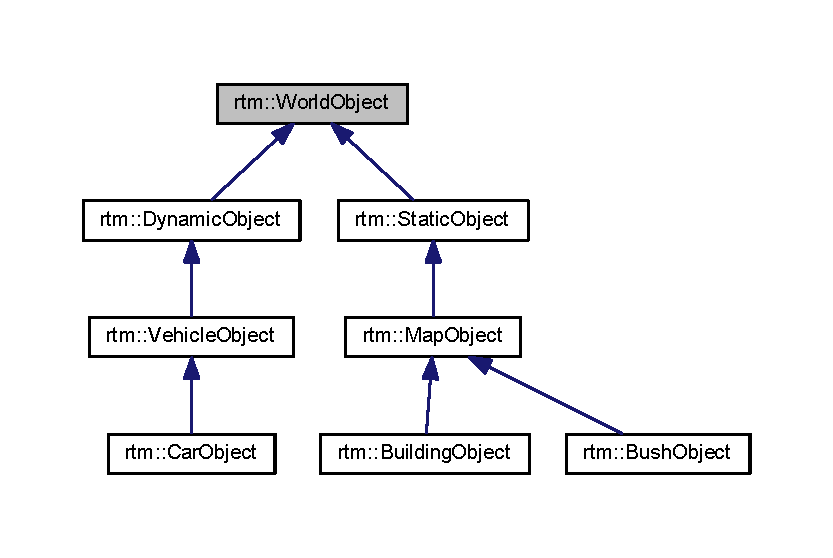
\includegraphics[width=350pt]{classrtm_1_1_world_object__inherit__graph}
\end{center}
\end{figure}
\subsection*{Открытые члены}
\begin{DoxyCompactItemize}
\item 
\mbox{\Hypertarget{classrtm_1_1_world_object_af44479be3cee7dd4de4d197adbb5afab}\label{classrtm_1_1_world_object_af44479be3cee7dd4de4d197adbb5afab}} 
\hyperlink{classrtm_1_1_world_object_af44479be3cee7dd4de4d197adbb5afab}{World\+Object} ()
\begin{DoxyCompactList}\small\item\em Конструктор по умолчанию \end{DoxyCompactList}\item 
\hyperlink{classrtm_1_1_world_object_a1a1196480079afe397f64055f333f83c}{World\+Object} (cocos2d\+::\+Sprite $\ast$const sprite, float x, float y, float angle)
\begin{DoxyCompactList}\small\item\em Конструктор с использованием уже готового спрайта \end{DoxyCompactList}\item 
\hyperlink{classrtm_1_1_world_object_a4462c860b41708d4570352dc3372064e}{World\+Object} (std\+::string const \&filename, float x, float y, float angle)
\begin{DoxyCompactList}\small\item\em Конструктор из файла \end{DoxyCompactList}\item 
\mbox{\Hypertarget{classrtm_1_1_world_object_a06dbc49bfcfa403a842ebe1f316763e0}\label{classrtm_1_1_world_object_a06dbc49bfcfa403a842ebe1f316763e0}} 
virtual \hyperlink{classrtm_1_1_world_object_a06dbc49bfcfa403a842ebe1f316763e0}{$\sim$\+World\+Object} ()=default
\begin{DoxyCompactList}\small\item\em Деструктор по умолчанию \end{DoxyCompactList}\item 
cocos2d\+::\+Sprite $\ast$ \hyperlink{classrtm_1_1_world_object_af0284b8fdc5a7ff8893d020d630a7fe5}{Get\+Sprite} () const
\begin{DoxyCompactList}\small\item\em Функция для получения спрайта \end{DoxyCompactList}\item 
float \hyperlink{classrtm_1_1_world_object_a31f148a74be54e4f1ccbf41fc8424552}{Get\+X\+\_\+} () const
\begin{DoxyCompactList}\small\item\em Функция для получения абсциссы \end{DoxyCompactList}\item 
float \hyperlink{classrtm_1_1_world_object_af558d23ff82794c8ace17b8aeefaf5bb}{Get\+Y\+\_\+} () const
\begin{DoxyCompactList}\small\item\em Функция для получения ординаты \end{DoxyCompactList}\item 
float \hyperlink{classrtm_1_1_world_object_ae9af0e03a3f49720b38ec69191c8d237}{Get\+Angle} () const
\begin{DoxyCompactList}\small\item\em Функция для получения угла поворота \end{DoxyCompactList}\item 
float \hyperlink{classrtm_1_1_world_object_a36a9cf3cce5c76f88164e0c790675a1e}{Get\+Width} () const
\begin{DoxyCompactList}\small\item\em Функция для получения ширины \end{DoxyCompactList}\item 
float \hyperlink{classrtm_1_1_world_object_ac1ab514e4556b3d8b9d4ffda5eba9db2}{Get\+Height} () const
\begin{DoxyCompactList}\small\item\em Функция для получения высоты \end{DoxyCompactList}\end{DoxyCompactItemize}
\subsection*{Защищенные члены}
\begin{DoxyCompactItemize}
\item 
void \hyperlink{classrtm_1_1_world_object_ae8f0605c11c95bf6eae8f42c24fc4130}{Set\+Sprite\+\_\+} (cocos2d\+::\+Sprite $\ast$const sprite)
\begin{DoxyCompactList}\small\item\em Функция для установки спрайта \end{DoxyCompactList}\item 
void \hyperlink{classrtm_1_1_world_object_a66fcf7be3345584be9f06e00a79da559}{Set\+X\+\_\+} (float x)
\begin{DoxyCompactList}\small\item\em Функция для установки абсциссы \end{DoxyCompactList}\item 
void \hyperlink{classrtm_1_1_world_object_a2d9de0f03e711f7b2486889d7336c9d3}{Set\+Y\+\_\+} (float y)
\begin{DoxyCompactList}\small\item\em Функция для установки ординаты \end{DoxyCompactList}\item 
void \hyperlink{classrtm_1_1_world_object_a3185c36d5138dde6f6942b101586cee4}{Set\+Angle\+\_\+} (float angle)
\begin{DoxyCompactList}\small\item\em Функция для установки угла поворота \end{DoxyCompactList}\item 
void \hyperlink{classrtm_1_1_world_object_ad11ace9402b562b5c2aa6817c4b1cc9f}{Set\+Width\+\_\+} (float width)
\begin{DoxyCompactList}\small\item\em Функция для установки ширины \end{DoxyCompactList}\item 
void \hyperlink{classrtm_1_1_world_object_a60904037c13f9cf151cd28f040ac5f02}{Set\+Height\+\_\+} (float height)
\begin{DoxyCompactList}\small\item\em Функция для установки высоты \end{DoxyCompactList}\item 
\mbox{\Hypertarget{classrtm_1_1_world_object_a4adc266618f3aeb94ae55df76f0716dc}\label{classrtm_1_1_world_object_a4adc266618f3aeb94ae55df76f0716dc}} 
virtual void \hyperlink{classrtm_1_1_world_object_a4adc266618f3aeb94ae55df76f0716dc}{Position\+Init\+\_\+} ()
\begin{DoxyCompactList}\small\item\em Функция, выполняемая во время инициализации \end{DoxyCompactList}\item 
\mbox{\Hypertarget{classrtm_1_1_world_object_a1619ffa3020e1cf19c901635fd3c4b88}\label{classrtm_1_1_world_object_a1619ffa3020e1cf19c901635fd3c4b88}} 
virtual void \hyperlink{classrtm_1_1_world_object_a1619ffa3020e1cf19c901635fd3c4b88}{Position\+Update\+\_\+} ()
\begin{DoxyCompactList}\small\item\em Функция, выполняемая во время обновления положения \end{DoxyCompactList}\item 
\mbox{\Hypertarget{classrtm_1_1_world_object_ac1094406fc176bd4ae14dfb3f081b7f5}\label{classrtm_1_1_world_object_ac1094406fc176bd4ae14dfb3f081b7f5}} 
virtual void \hyperlink{classrtm_1_1_world_object_ac1094406fc176bd4ae14dfb3f081b7f5}{On\+X\+Update\+\_\+} ()
\begin{DoxyCompactList}\small\item\em Функция, выполняемая во время обновления абсциссы \end{DoxyCompactList}\item 
\mbox{\Hypertarget{classrtm_1_1_world_object_ad6e57a1a4696307449bdd9376bfcdd75}\label{classrtm_1_1_world_object_ad6e57a1a4696307449bdd9376bfcdd75}} 
virtual void \hyperlink{classrtm_1_1_world_object_ad6e57a1a4696307449bdd9376bfcdd75}{On\+Y\+Update\+\_\+} ()
\begin{DoxyCompactList}\small\item\em Функция, выполняемая во время обновления ординаты \end{DoxyCompactList}\item 
\mbox{\Hypertarget{classrtm_1_1_world_object_aeaf9640864189b88f41a4ea24ef8b5f9}\label{classrtm_1_1_world_object_aeaf9640864189b88f41a4ea24ef8b5f9}} 
virtual void \hyperlink{classrtm_1_1_world_object_aeaf9640864189b88f41a4ea24ef8b5f9}{On\+Angle\+Update\+\_\+} ()
\begin{DoxyCompactList}\small\item\em Функция, выполняемая во время обновления угла поворота \end{DoxyCompactList}\item 
\mbox{\Hypertarget{classrtm_1_1_world_object_acb07848ff4e36ac3b77a6c2aea2f6547}\label{classrtm_1_1_world_object_acb07848ff4e36ac3b77a6c2aea2f6547}} 
virtual void \hyperlink{classrtm_1_1_world_object_acb07848ff4e36ac3b77a6c2aea2f6547}{On\+Width\+Update\+\_\+} ()
\begin{DoxyCompactList}\small\item\em Функция, выполняемая во время обновления ширины \end{DoxyCompactList}\item 
\mbox{\Hypertarget{classrtm_1_1_world_object_a3261c4ad76d199370db74a4fd09ddf29}\label{classrtm_1_1_world_object_a3261c4ad76d199370db74a4fd09ddf29}} 
virtual void \hyperlink{classrtm_1_1_world_object_a3261c4ad76d199370db74a4fd09ddf29}{On\+Height\+Update\+\_\+} ()
\begin{DoxyCompactList}\small\item\em Функция, выполняемая во время обновления высоты \end{DoxyCompactList}\end{DoxyCompactItemize}
\subsection*{Закрытые члены}
\begin{DoxyCompactItemize}
\item 
void \hyperlink{classrtm_1_1_world_object_a57de67f0e2788f0b3226beb2b84a5551}{Set\+Sprite\+X\+\_\+} (float x)
\begin{DoxyCompactList}\small\item\em Функция для установки абсциссы спрайта \end{DoxyCompactList}\item 
void \hyperlink{classrtm_1_1_world_object_a885eff01e5b07ef96194a868ff1fe338}{Set\+Sprite\+Y\+\_\+} (float y)
\begin{DoxyCompactList}\small\item\em Функция для установки ординаты спрайта \end{DoxyCompactList}\item 
void \hyperlink{classrtm_1_1_world_object_a5daee1cc41f0657f33d6790c22614f5e}{Set\+Sprite\+Angle\+\_\+} (float angle)
\begin{DoxyCompactList}\small\item\em Функция для установки угла поворота спрайта \end{DoxyCompactList}\item 
void \hyperlink{classrtm_1_1_world_object_a2a88c51a636b8b8c94320c0f6d66feb7}{Set\+Sprite\+Width\+\_\+} (float width)
\begin{DoxyCompactList}\small\item\em Функция для установки ширины спрайта \end{DoxyCompactList}\item 
void \hyperlink{classrtm_1_1_world_object_a553abd97f4f63659282f1e903dfc074b}{Set\+Sprite\+Height\+\_\+} (float height)
\begin{DoxyCompactList}\small\item\em Функция для установки высоты спрайта \end{DoxyCompactList}\end{DoxyCompactItemize}
\subsection*{Закрытые данные}
\begin{DoxyCompactItemize}
\item 
\mbox{\Hypertarget{classrtm_1_1_world_object_ab371756fde7d223a4ff6fc72d42c9cf0}\label{classrtm_1_1_world_object_ab371756fde7d223a4ff6fc72d42c9cf0}} 
cocos2d\+::\+Sprite $\ast$ \hyperlink{classrtm_1_1_world_object_ab371756fde7d223a4ff6fc72d42c9cf0}{sprite\+\_\+}
\begin{DoxyCompactList}\small\item\em Указатель на спрайт \end{DoxyCompactList}\item 
\mbox{\Hypertarget{classrtm_1_1_world_object_a719b4bdf8eeca018f95ff42d0599944e}\label{classrtm_1_1_world_object_a719b4bdf8eeca018f95ff42d0599944e}} 
float \hyperlink{classrtm_1_1_world_object_a719b4bdf8eeca018f95ff42d0599944e}{x\+\_\+}
\begin{DoxyCompactList}\small\item\em Абсцисса \end{DoxyCompactList}\item 
\mbox{\Hypertarget{classrtm_1_1_world_object_ab66518f51a9b063e94f4e082789fa032}\label{classrtm_1_1_world_object_ab66518f51a9b063e94f4e082789fa032}} 
float \hyperlink{classrtm_1_1_world_object_ab66518f51a9b063e94f4e082789fa032}{prev\+X\+\_\+}
\begin{DoxyCompactList}\small\item\em Абсцисса для отслеживания изменений \end{DoxyCompactList}\item 
\mbox{\Hypertarget{classrtm_1_1_world_object_a5d4541d2f052555a0ce07001da6fd04f}\label{classrtm_1_1_world_object_a5d4541d2f052555a0ce07001da6fd04f}} 
float \hyperlink{classrtm_1_1_world_object_a5d4541d2f052555a0ce07001da6fd04f}{y\+\_\+}
\begin{DoxyCompactList}\small\item\em Ордината \end{DoxyCompactList}\item 
\mbox{\Hypertarget{classrtm_1_1_world_object_aa9b38c50c7900db0fa7dec8c9a8d9086}\label{classrtm_1_1_world_object_aa9b38c50c7900db0fa7dec8c9a8d9086}} 
float \hyperlink{classrtm_1_1_world_object_aa9b38c50c7900db0fa7dec8c9a8d9086}{prev\+Y\+\_\+}
\begin{DoxyCompactList}\small\item\em Ордината для отслеживания изменений \end{DoxyCompactList}\item 
\mbox{\Hypertarget{classrtm_1_1_world_object_aaf64d1d04e4ef1bc481c5f79c99b68ba}\label{classrtm_1_1_world_object_aaf64d1d04e4ef1bc481c5f79c99b68ba}} 
float \hyperlink{classrtm_1_1_world_object_aaf64d1d04e4ef1bc481c5f79c99b68ba}{angle\+\_\+}
\begin{DoxyCompactList}\small\item\em Угол поворота \end{DoxyCompactList}\item 
\mbox{\Hypertarget{classrtm_1_1_world_object_acee095a4e2c8244346f0a7a5208fbd04}\label{classrtm_1_1_world_object_acee095a4e2c8244346f0a7a5208fbd04}} 
float \hyperlink{classrtm_1_1_world_object_acee095a4e2c8244346f0a7a5208fbd04}{prev\+Angle\+\_\+}
\begin{DoxyCompactList}\small\item\em Угол поворота для отслеживания изменений \end{DoxyCompactList}\item 
\mbox{\Hypertarget{classrtm_1_1_world_object_a80da665dd4334ad3dd8a33c7461b8436}\label{classrtm_1_1_world_object_a80da665dd4334ad3dd8a33c7461b8436}} 
float \hyperlink{classrtm_1_1_world_object_a80da665dd4334ad3dd8a33c7461b8436}{width\+\_\+}
\begin{DoxyCompactList}\small\item\em Ширина \end{DoxyCompactList}\item 
\mbox{\Hypertarget{classrtm_1_1_world_object_a9dd43ca401792997b814c174da40cec7}\label{classrtm_1_1_world_object_a9dd43ca401792997b814c174da40cec7}} 
float \hyperlink{classrtm_1_1_world_object_a9dd43ca401792997b814c174da40cec7}{prev\+Width\+\_\+}
\begin{DoxyCompactList}\small\item\em Ширина для отслеживания изменений \end{DoxyCompactList}\item 
\mbox{\Hypertarget{classrtm_1_1_world_object_a0efb406ca0273790ad607e1e87d1ce07}\label{classrtm_1_1_world_object_a0efb406ca0273790ad607e1e87d1ce07}} 
float \hyperlink{classrtm_1_1_world_object_a0efb406ca0273790ad607e1e87d1ce07}{height\+\_\+}
\begin{DoxyCompactList}\small\item\em Высота \end{DoxyCompactList}\item 
\mbox{\Hypertarget{classrtm_1_1_world_object_a1b08d1adfefde6d956f382418c06c49e}\label{classrtm_1_1_world_object_a1b08d1adfefde6d956f382418c06c49e}} 
float \hyperlink{classrtm_1_1_world_object_a1b08d1adfefde6d956f382418c06c49e}{prev\+Height\+\_\+}
\begin{DoxyCompactList}\small\item\em Высота для отслеживания изменений \end{DoxyCompactList}\end{DoxyCompactItemize}


\subsection{Подробное описание}
Класс объекта мира (родитель всех условно объемных объектов) 

\subsection{Конструктор(ы)}
\mbox{\Hypertarget{classrtm_1_1_world_object_a1a1196480079afe397f64055f333f83c}\label{classrtm_1_1_world_object_a1a1196480079afe397f64055f333f83c}} 
\index{rtm\+::\+World\+Object@{rtm\+::\+World\+Object}!World\+Object@{World\+Object}}
\index{World\+Object@{World\+Object}!rtm\+::\+World\+Object@{rtm\+::\+World\+Object}}
\subsubsection{\texorpdfstring{World\+Object()}{WorldObject()}\hspace{0.1cm}{\footnotesize\ttfamily [1/2]}}
{\footnotesize\ttfamily rtm\+::\+World\+Object\+::\+World\+Object (\begin{DoxyParamCaption}\item[{cocos2d\+::\+Sprite $\ast$const}]{sprite,  }\item[{float}]{x,  }\item[{float}]{y,  }\item[{float}]{angle }\end{DoxyParamCaption})}



Конструктор с использованием уже готового спрайта 


\begin{DoxyParams}{Аргументы}
{\em sprite} & указатель на готовый спрайт \\
\hline
{\em x} & абсцисса \\
\hline
{\em y} & ордината \\
\hline
{\em angle} & угол поворота объекта \\
\hline
\end{DoxyParams}
\mbox{\Hypertarget{classrtm_1_1_world_object_a4462c860b41708d4570352dc3372064e}\label{classrtm_1_1_world_object_a4462c860b41708d4570352dc3372064e}} 
\index{rtm\+::\+World\+Object@{rtm\+::\+World\+Object}!World\+Object@{World\+Object}}
\index{World\+Object@{World\+Object}!rtm\+::\+World\+Object@{rtm\+::\+World\+Object}}
\subsubsection{\texorpdfstring{World\+Object()}{WorldObject()}\hspace{0.1cm}{\footnotesize\ttfamily [2/2]}}
{\footnotesize\ttfamily rtm\+::\+World\+Object\+::\+World\+Object (\begin{DoxyParamCaption}\item[{std\+::string const \&}]{filename,  }\item[{float}]{x,  }\item[{float}]{y,  }\item[{float}]{angle }\end{DoxyParamCaption})}



Конструктор из файла 


\begin{DoxyParams}{Аргументы}
{\em filename} & путь к файлу инициализации \\
\hline
{\em x} & абсцисса \\
\hline
{\em y} & ордината \\
\hline
{\em angle} & угол поворота объекта \\
\hline
\end{DoxyParams}


\subsection{Методы}
\mbox{\Hypertarget{classrtm_1_1_world_object_af0284b8fdc5a7ff8893d020d630a7fe5}\label{classrtm_1_1_world_object_af0284b8fdc5a7ff8893d020d630a7fe5}} 
\index{rtm\+::\+World\+Object@{rtm\+::\+World\+Object}!Get\+Sprite@{Get\+Sprite}}
\index{Get\+Sprite@{Get\+Sprite}!rtm\+::\+World\+Object@{rtm\+::\+World\+Object}}
\subsubsection{\texorpdfstring{Get\+Sprite()}{GetSprite()}}
{\footnotesize\ttfamily cocos2d\+::\+Sprite $\ast$ rtm\+::\+World\+Object\+::\+Get\+Sprite (\begin{DoxyParamCaption}{ }\end{DoxyParamCaption}) const}



Функция для получения спрайта 

\begin{DoxyReturn}{Возвращает}
указатель на спрайт 
\end{DoxyReturn}
\mbox{\Hypertarget{classrtm_1_1_world_object_a31f148a74be54e4f1ccbf41fc8424552}\label{classrtm_1_1_world_object_a31f148a74be54e4f1ccbf41fc8424552}} 
\index{rtm\+::\+World\+Object@{rtm\+::\+World\+Object}!Get\+X\+\_\+@{Get\+X\+\_\+}}
\index{Get\+X\+\_\+@{Get\+X\+\_\+}!rtm\+::\+World\+Object@{rtm\+::\+World\+Object}}
\subsubsection{\texorpdfstring{Get\+X\+\_\+()}{GetX\_()}}
{\footnotesize\ttfamily float rtm\+::\+World\+Object\+::\+Get\+X\+\_\+ (\begin{DoxyParamCaption}{ }\end{DoxyParamCaption}) const}



Функция для получения абсциссы 

\begin{DoxyReturn}{Возвращает}
абсцисса 
\end{DoxyReturn}
\mbox{\Hypertarget{classrtm_1_1_world_object_af558d23ff82794c8ace17b8aeefaf5bb}\label{classrtm_1_1_world_object_af558d23ff82794c8ace17b8aeefaf5bb}} 
\index{rtm\+::\+World\+Object@{rtm\+::\+World\+Object}!Get\+Y\+\_\+@{Get\+Y\+\_\+}}
\index{Get\+Y\+\_\+@{Get\+Y\+\_\+}!rtm\+::\+World\+Object@{rtm\+::\+World\+Object}}
\subsubsection{\texorpdfstring{Get\+Y\+\_\+()}{GetY\_()}}
{\footnotesize\ttfamily float rtm\+::\+World\+Object\+::\+Get\+Y\+\_\+ (\begin{DoxyParamCaption}{ }\end{DoxyParamCaption}) const}



Функция для получения ординаты 

\begin{DoxyReturn}{Возвращает}
ордината 
\end{DoxyReturn}
\mbox{\Hypertarget{classrtm_1_1_world_object_ae9af0e03a3f49720b38ec69191c8d237}\label{classrtm_1_1_world_object_ae9af0e03a3f49720b38ec69191c8d237}} 
\index{rtm\+::\+World\+Object@{rtm\+::\+World\+Object}!Get\+Angle@{Get\+Angle}}
\index{Get\+Angle@{Get\+Angle}!rtm\+::\+World\+Object@{rtm\+::\+World\+Object}}
\subsubsection{\texorpdfstring{Get\+Angle()}{GetAngle()}}
{\footnotesize\ttfamily float rtm\+::\+World\+Object\+::\+Get\+Angle (\begin{DoxyParamCaption}{ }\end{DoxyParamCaption}) const}



Функция для получения угла поворота 

\begin{DoxyReturn}{Возвращает}
угол поворота 
\end{DoxyReturn}
\mbox{\Hypertarget{classrtm_1_1_world_object_a36a9cf3cce5c76f88164e0c790675a1e}\label{classrtm_1_1_world_object_a36a9cf3cce5c76f88164e0c790675a1e}} 
\index{rtm\+::\+World\+Object@{rtm\+::\+World\+Object}!Get\+Width@{Get\+Width}}
\index{Get\+Width@{Get\+Width}!rtm\+::\+World\+Object@{rtm\+::\+World\+Object}}
\subsubsection{\texorpdfstring{Get\+Width()}{GetWidth()}}
{\footnotesize\ttfamily float rtm\+::\+World\+Object\+::\+Get\+Width (\begin{DoxyParamCaption}{ }\end{DoxyParamCaption}) const}



Функция для получения ширины 

\begin{DoxyReturn}{Возвращает}
ширина 
\end{DoxyReturn}
\mbox{\Hypertarget{classrtm_1_1_world_object_ac1ab514e4556b3d8b9d4ffda5eba9db2}\label{classrtm_1_1_world_object_ac1ab514e4556b3d8b9d4ffda5eba9db2}} 
\index{rtm\+::\+World\+Object@{rtm\+::\+World\+Object}!Get\+Height@{Get\+Height}}
\index{Get\+Height@{Get\+Height}!rtm\+::\+World\+Object@{rtm\+::\+World\+Object}}
\subsubsection{\texorpdfstring{Get\+Height()}{GetHeight()}}
{\footnotesize\ttfamily float rtm\+::\+World\+Object\+::\+Get\+Height (\begin{DoxyParamCaption}{ }\end{DoxyParamCaption}) const}



Функция для получения высоты 

\begin{DoxyReturn}{Возвращает}
высота 
\end{DoxyReturn}
\mbox{\Hypertarget{classrtm_1_1_world_object_ae8f0605c11c95bf6eae8f42c24fc4130}\label{classrtm_1_1_world_object_ae8f0605c11c95bf6eae8f42c24fc4130}} 
\index{rtm\+::\+World\+Object@{rtm\+::\+World\+Object}!Set\+Sprite\+\_\+@{Set\+Sprite\+\_\+}}
\index{Set\+Sprite\+\_\+@{Set\+Sprite\+\_\+}!rtm\+::\+World\+Object@{rtm\+::\+World\+Object}}
\subsubsection{\texorpdfstring{Set\+Sprite\+\_\+()}{SetSprite\_()}}
{\footnotesize\ttfamily void rtm\+::\+World\+Object\+::\+Set\+Sprite\+\_\+ (\begin{DoxyParamCaption}\item[{cocos2d\+::\+Sprite $\ast$const}]{sprite }\end{DoxyParamCaption})\hspace{0.3cm}{\ttfamily [protected]}}



Функция для установки спрайта 


\begin{DoxyParams}{Аргументы}
{\em sprite} & указатель на спрайт \\
\hline
\end{DoxyParams}
\mbox{\Hypertarget{classrtm_1_1_world_object_a66fcf7be3345584be9f06e00a79da559}\label{classrtm_1_1_world_object_a66fcf7be3345584be9f06e00a79da559}} 
\index{rtm\+::\+World\+Object@{rtm\+::\+World\+Object}!Set\+X\+\_\+@{Set\+X\+\_\+}}
\index{Set\+X\+\_\+@{Set\+X\+\_\+}!rtm\+::\+World\+Object@{rtm\+::\+World\+Object}}
\subsubsection{\texorpdfstring{Set\+X\+\_\+()}{SetX\_()}}
{\footnotesize\ttfamily void rtm\+::\+World\+Object\+::\+Set\+X\+\_\+ (\begin{DoxyParamCaption}\item[{float}]{x }\end{DoxyParamCaption})\hspace{0.3cm}{\ttfamily [protected]}}



Функция для установки абсциссы 


\begin{DoxyParams}{Аргументы}
{\em x} & абсцисса \\
\hline
\end{DoxyParams}
\mbox{\Hypertarget{classrtm_1_1_world_object_a2d9de0f03e711f7b2486889d7336c9d3}\label{classrtm_1_1_world_object_a2d9de0f03e711f7b2486889d7336c9d3}} 
\index{rtm\+::\+World\+Object@{rtm\+::\+World\+Object}!Set\+Y\+\_\+@{Set\+Y\+\_\+}}
\index{Set\+Y\+\_\+@{Set\+Y\+\_\+}!rtm\+::\+World\+Object@{rtm\+::\+World\+Object}}
\subsubsection{\texorpdfstring{Set\+Y\+\_\+()}{SetY\_()}}
{\footnotesize\ttfamily void rtm\+::\+World\+Object\+::\+Set\+Y\+\_\+ (\begin{DoxyParamCaption}\item[{float}]{y }\end{DoxyParamCaption})\hspace{0.3cm}{\ttfamily [protected]}}



Функция для установки ординаты 


\begin{DoxyParams}{Аргументы}
{\em y} & ордината \\
\hline
\end{DoxyParams}
\mbox{\Hypertarget{classrtm_1_1_world_object_a3185c36d5138dde6f6942b101586cee4}\label{classrtm_1_1_world_object_a3185c36d5138dde6f6942b101586cee4}} 
\index{rtm\+::\+World\+Object@{rtm\+::\+World\+Object}!Set\+Angle\+\_\+@{Set\+Angle\+\_\+}}
\index{Set\+Angle\+\_\+@{Set\+Angle\+\_\+}!rtm\+::\+World\+Object@{rtm\+::\+World\+Object}}
\subsubsection{\texorpdfstring{Set\+Angle\+\_\+()}{SetAngle\_()}}
{\footnotesize\ttfamily void rtm\+::\+World\+Object\+::\+Set\+Angle\+\_\+ (\begin{DoxyParamCaption}\item[{float}]{angle }\end{DoxyParamCaption})\hspace{0.3cm}{\ttfamily [protected]}}



Функция для установки угла поворота 


\begin{DoxyParams}{Аргументы}
{\em angle} & угол поворота \\
\hline
\end{DoxyParams}
\mbox{\Hypertarget{classrtm_1_1_world_object_ad11ace9402b562b5c2aa6817c4b1cc9f}\label{classrtm_1_1_world_object_ad11ace9402b562b5c2aa6817c4b1cc9f}} 
\index{rtm\+::\+World\+Object@{rtm\+::\+World\+Object}!Set\+Width\+\_\+@{Set\+Width\+\_\+}}
\index{Set\+Width\+\_\+@{Set\+Width\+\_\+}!rtm\+::\+World\+Object@{rtm\+::\+World\+Object}}
\subsubsection{\texorpdfstring{Set\+Width\+\_\+()}{SetWidth\_()}}
{\footnotesize\ttfamily void rtm\+::\+World\+Object\+::\+Set\+Width\+\_\+ (\begin{DoxyParamCaption}\item[{float}]{width }\end{DoxyParamCaption})\hspace{0.3cm}{\ttfamily [protected]}}



Функция для установки ширины 


\begin{DoxyParams}{Аргументы}
{\em width} & ширина \\
\hline
\end{DoxyParams}
\mbox{\Hypertarget{classrtm_1_1_world_object_a60904037c13f9cf151cd28f040ac5f02}\label{classrtm_1_1_world_object_a60904037c13f9cf151cd28f040ac5f02}} 
\index{rtm\+::\+World\+Object@{rtm\+::\+World\+Object}!Set\+Height\+\_\+@{Set\+Height\+\_\+}}
\index{Set\+Height\+\_\+@{Set\+Height\+\_\+}!rtm\+::\+World\+Object@{rtm\+::\+World\+Object}}
\subsubsection{\texorpdfstring{Set\+Height\+\_\+()}{SetHeight\_()}}
{\footnotesize\ttfamily void rtm\+::\+World\+Object\+::\+Set\+Height\+\_\+ (\begin{DoxyParamCaption}\item[{float}]{height }\end{DoxyParamCaption})\hspace{0.3cm}{\ttfamily [protected]}}



Функция для установки высоты 


\begin{DoxyParams}{Аргументы}
{\em height} & высота \\
\hline
\end{DoxyParams}
\mbox{\Hypertarget{classrtm_1_1_world_object_a57de67f0e2788f0b3226beb2b84a5551}\label{classrtm_1_1_world_object_a57de67f0e2788f0b3226beb2b84a5551}} 
\index{rtm\+::\+World\+Object@{rtm\+::\+World\+Object}!Set\+Sprite\+X\+\_\+@{Set\+Sprite\+X\+\_\+}}
\index{Set\+Sprite\+X\+\_\+@{Set\+Sprite\+X\+\_\+}!rtm\+::\+World\+Object@{rtm\+::\+World\+Object}}
\subsubsection{\texorpdfstring{Set\+Sprite\+X\+\_\+()}{SetSpriteX\_()}}
{\footnotesize\ttfamily void rtm\+::\+World\+Object\+::\+Set\+Sprite\+X\+\_\+ (\begin{DoxyParamCaption}\item[{float}]{x }\end{DoxyParamCaption})\hspace{0.3cm}{\ttfamily [private]}}



Функция для установки абсциссы спрайта 


\begin{DoxyParams}{Аргументы}
{\em x} & абсцисса спрайта \\
\hline
\end{DoxyParams}
\mbox{\Hypertarget{classrtm_1_1_world_object_a885eff01e5b07ef96194a868ff1fe338}\label{classrtm_1_1_world_object_a885eff01e5b07ef96194a868ff1fe338}} 
\index{rtm\+::\+World\+Object@{rtm\+::\+World\+Object}!Set\+Sprite\+Y\+\_\+@{Set\+Sprite\+Y\+\_\+}}
\index{Set\+Sprite\+Y\+\_\+@{Set\+Sprite\+Y\+\_\+}!rtm\+::\+World\+Object@{rtm\+::\+World\+Object}}
\subsubsection{\texorpdfstring{Set\+Sprite\+Y\+\_\+()}{SetSpriteY\_()}}
{\footnotesize\ttfamily void rtm\+::\+World\+Object\+::\+Set\+Sprite\+Y\+\_\+ (\begin{DoxyParamCaption}\item[{float}]{y }\end{DoxyParamCaption})\hspace{0.3cm}{\ttfamily [private]}}



Функция для установки ординаты спрайта 


\begin{DoxyParams}{Аргументы}
{\em y} & ордината спрайта \\
\hline
\end{DoxyParams}
\mbox{\Hypertarget{classrtm_1_1_world_object_a5daee1cc41f0657f33d6790c22614f5e}\label{classrtm_1_1_world_object_a5daee1cc41f0657f33d6790c22614f5e}} 
\index{rtm\+::\+World\+Object@{rtm\+::\+World\+Object}!Set\+Sprite\+Angle\+\_\+@{Set\+Sprite\+Angle\+\_\+}}
\index{Set\+Sprite\+Angle\+\_\+@{Set\+Sprite\+Angle\+\_\+}!rtm\+::\+World\+Object@{rtm\+::\+World\+Object}}
\subsubsection{\texorpdfstring{Set\+Sprite\+Angle\+\_\+()}{SetSpriteAngle\_()}}
{\footnotesize\ttfamily void rtm\+::\+World\+Object\+::\+Set\+Sprite\+Angle\+\_\+ (\begin{DoxyParamCaption}\item[{float}]{angle }\end{DoxyParamCaption})\hspace{0.3cm}{\ttfamily [private]}}



Функция для установки угла поворота спрайта 


\begin{DoxyParams}{Аргументы}
{\em angle} & угол поворота спрайта \\
\hline
\end{DoxyParams}
\mbox{\Hypertarget{classrtm_1_1_world_object_a2a88c51a636b8b8c94320c0f6d66feb7}\label{classrtm_1_1_world_object_a2a88c51a636b8b8c94320c0f6d66feb7}} 
\index{rtm\+::\+World\+Object@{rtm\+::\+World\+Object}!Set\+Sprite\+Width\+\_\+@{Set\+Sprite\+Width\+\_\+}}
\index{Set\+Sprite\+Width\+\_\+@{Set\+Sprite\+Width\+\_\+}!rtm\+::\+World\+Object@{rtm\+::\+World\+Object}}
\subsubsection{\texorpdfstring{Set\+Sprite\+Width\+\_\+()}{SetSpriteWidth\_()}}
{\footnotesize\ttfamily void rtm\+::\+World\+Object\+::\+Set\+Sprite\+Width\+\_\+ (\begin{DoxyParamCaption}\item[{float}]{width }\end{DoxyParamCaption})\hspace{0.3cm}{\ttfamily [private]}}



Функция для установки ширины спрайта 


\begin{DoxyParams}{Аргументы}
{\em width} & ширина спрайта \\
\hline
\end{DoxyParams}
\mbox{\Hypertarget{classrtm_1_1_world_object_a553abd97f4f63659282f1e903dfc074b}\label{classrtm_1_1_world_object_a553abd97f4f63659282f1e903dfc074b}} 
\index{rtm\+::\+World\+Object@{rtm\+::\+World\+Object}!Set\+Sprite\+Height\+\_\+@{Set\+Sprite\+Height\+\_\+}}
\index{Set\+Sprite\+Height\+\_\+@{Set\+Sprite\+Height\+\_\+}!rtm\+::\+World\+Object@{rtm\+::\+World\+Object}}
\subsubsection{\texorpdfstring{Set\+Sprite\+Height\+\_\+()}{SetSpriteHeight\_()}}
{\footnotesize\ttfamily void rtm\+::\+World\+Object\+::\+Set\+Sprite\+Height\+\_\+ (\begin{DoxyParamCaption}\item[{float}]{height }\end{DoxyParamCaption})\hspace{0.3cm}{\ttfamily [private]}}



Функция для установки высоты спрайта 


\begin{DoxyParams}{Аргументы}
{\em height} & высота спрайта \\
\hline
\end{DoxyParams}


Объявления и описания членов классов находятся в файлах\+:\begin{DoxyCompactItemize}
\item 
C\+:/\+Users/\+Vladimir/\+Documents/\+Visual Studio 2017/\+Projects/\+R\+T\+M/\+Classes/World\+Object.\+h\item 
C\+:/\+Users/\+Vladimir/\+Documents/\+Visual Studio 2017/\+Projects/\+R\+T\+M/\+Classes/World\+Object.\+cpp\end{DoxyCompactItemize}

\hypertarget{classrtm_1_1_world_scene}{}\section{Класс rtm\+:\+:World\+Scene}
\label{classrtm_1_1_world_scene}\index{rtm\+::\+World\+Scene@{rtm\+::\+World\+Scene}}


Класс главной сцены, на которой всё и происходит (для отрисовки)  




{\ttfamily \#include $<$World\+Scene.\+h$>$}



Граф наследования\+:rtm\+:\+:World\+Scene\+:
\nopagebreak
\begin{figure}[H]
\begin{center}
\leavevmode
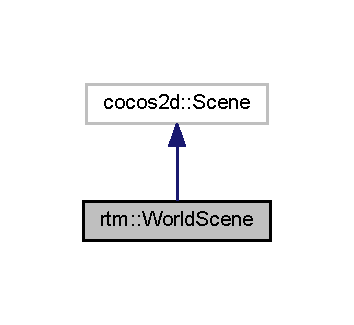
\includegraphics[width=170pt]{classrtm_1_1_world_scene__inherit__graph}
\end{center}
\end{figure}
\subsection*{Открытые члены}
\begin{DoxyCompactItemize}
\item 
\mbox{\Hypertarget{classrtm_1_1_world_scene_a0e7f98986330555b5fcecf218915e623}\label{classrtm_1_1_world_scene_a0e7f98986330555b5fcecf218915e623}} 
\hyperlink{classrtm_1_1_world_scene_a0e7f98986330555b5fcecf218915e623}{$\sim$\+World\+Scene} ()=default
\begin{DoxyCompactList}\small\item\em Деструктор по умолчанию \end{DoxyCompactList}\item 
virtual bool \hyperlink{classrtm_1_1_world_scene_a53da1782e50b99e90831bceb54c69ab9}{init} () override
\begin{DoxyCompactList}\small\item\em Функция для инициализации полей \end{DoxyCompactList}\item 
virtual void \hyperlink{classrtm_1_1_world_scene_a243c2d00cc0e525738b099eea7120fba}{update} (float time) override
\begin{DoxyCompactList}\small\item\em Функция для обновления сцены \end{DoxyCompactList}\item 
cocos2d\+::\+Layer $\ast$ \hyperlink{classrtm_1_1_world_scene_a33b06df7f231db363d6894408e16e225}{Get\+Main\+Layer} () const
\begin{DoxyCompactList}\small\item\em Функция для получения основного слоя, на котором находятся объекты \end{DoxyCompactList}\end{DoxyCompactItemize}
\begin{Indent}\textbf{ Функции для установки фона}\par
\begin{DoxyCompactItemize}
\item 
void \hyperlink{classrtm_1_1_world_scene_accf4ad079366ad6ca9731bff83d937c0}{Set\+Background} (std\+::string const \&filename)
\begin{DoxyCompactList}\small\item\em Функции для установки фона из файла \end{DoxyCompactList}\item 
void \hyperlink{classrtm_1_1_world_scene_a097fa828c003f8757faf1aebdd0e63f1}{Set\+Background} (size\+\_\+t number)
\begin{DoxyCompactList}\small\item\em Функции для установки фона по номеру \end{DoxyCompactList}\end{DoxyCompactItemize}
\end{Indent}
\subsection*{Открытые статические члены}
\begin{DoxyCompactItemize}
\item 
static \hyperlink{classrtm_1_1_world_scene}{World\+Scene} $\ast$ \hyperlink{classrtm_1_1_world_scene_a4d9c6dcf1fc6a02c1d090caed0ad6745}{Create} ()
\begin{DoxyCompactList}\small\item\em Конструктор класса, поддерживающий R\+A\+II. \end{DoxyCompactList}\end{DoxyCompactItemize}
\subsection*{Закрытые члены}
\begin{DoxyCompactItemize}
\item 
\mbox{\Hypertarget{classrtm_1_1_world_scene_ac7b1c0b254cec69702731656e956408c}\label{classrtm_1_1_world_scene_ac7b1c0b254cec69702731656e956408c}} 
void \hyperlink{classrtm_1_1_world_scene_ac7b1c0b254cec69702731656e956408c}{Open\+Map\+\_\+} ()
\begin{DoxyCompactList}\small\item\em Функция открытия карты \end{DoxyCompactList}\item 
\mbox{\Hypertarget{classrtm_1_1_world_scene_acbad351934c371965ee9da74b3dba955}\label{classrtm_1_1_world_scene_acbad351934c371965ee9da74b3dba955}} 
void \hyperlink{classrtm_1_1_world_scene_acbad351934c371965ee9da74b3dba955}{Restart\+\_\+} ()
\begin{DoxyCompactList}\small\item\em Функция перезагрузки карты \end{DoxyCompactList}\item 
\mbox{\Hypertarget{classrtm_1_1_world_scene_aed8f5c4d5a0ff42e806adaf141da0cc7}\label{classrtm_1_1_world_scene_aed8f5c4d5a0ff42e806adaf141da0cc7}} 
void \hyperlink{classrtm_1_1_world_scene_aed8f5c4d5a0ff42e806adaf141da0cc7}{Set\+Default\+Position\+\_\+} ()
\begin{DoxyCompactList}\small\item\em Функция для установки первоначальной позиции просмотра \end{DoxyCompactList}\item 
\mbox{\Hypertarget{classrtm_1_1_world_scene_a60c760a9f665e3863a80d191be7de87b}\label{classrtm_1_1_world_scene_a60c760a9f665e3863a80d191be7de87b}} 
void \hyperlink{classrtm_1_1_world_scene_a60c760a9f665e3863a80d191be7de87b}{Shift\+Up\+\_\+} ()
\begin{DoxyCompactList}\small\item\em Функция сдвига области просмотра вверх \end{DoxyCompactList}\item 
\mbox{\Hypertarget{classrtm_1_1_world_scene_a125e4ae96bd562cc124a369929c49b21}\label{classrtm_1_1_world_scene_a125e4ae96bd562cc124a369929c49b21}} 
void \hyperlink{classrtm_1_1_world_scene_a125e4ae96bd562cc124a369929c49b21}{Shift\+Right\+\_\+} ()
\begin{DoxyCompactList}\small\item\em Функция сдвига области просмотра вправо \end{DoxyCompactList}\item 
\mbox{\Hypertarget{classrtm_1_1_world_scene_a1add96021d1be8d8d7010b54b5cdcd39}\label{classrtm_1_1_world_scene_a1add96021d1be8d8d7010b54b5cdcd39}} 
void \hyperlink{classrtm_1_1_world_scene_a1add96021d1be8d8d7010b54b5cdcd39}{Shift\+Down\+\_\+} ()
\begin{DoxyCompactList}\small\item\em Функция сдвига области просмотра вниз \end{DoxyCompactList}\item 
\mbox{\Hypertarget{classrtm_1_1_world_scene_ad0925929f7cabc77b9ce5fafc9ad46ff}\label{classrtm_1_1_world_scene_ad0925929f7cabc77b9ce5fafc9ad46ff}} 
void \hyperlink{classrtm_1_1_world_scene_ad0925929f7cabc77b9ce5fafc9ad46ff}{Shift\+Left\+\_\+} ()
\begin{DoxyCompactList}\small\item\em Функция сдвига области просмотра влево \end{DoxyCompactList}\item 
\mbox{\Hypertarget{classrtm_1_1_world_scene_a8d27585fd9c96bace0fc38a3f2d4fb35}\label{classrtm_1_1_world_scene_a8d27585fd9c96bace0fc38a3f2d4fb35}} 
void \hyperlink{classrtm_1_1_world_scene_a8d27585fd9c96bace0fc38a3f2d4fb35}{Update\+Position\+\_\+} ()
\begin{DoxyCompactList}\small\item\em Функция для обновления положения главного слоя в зависимости от области просмотра \end{DoxyCompactList}\item 
\mbox{\Hypertarget{classrtm_1_1_world_scene_ada5bb74ead734e654e21186f8f23b997}\label{classrtm_1_1_world_scene_ada5bb74ead734e654e21186f8f23b997}} 
void \hyperlink{classrtm_1_1_world_scene_ada5bb74ead734e654e21186f8f23b997}{Set\+Default\+Scale\+\_\+} ()
\begin{DoxyCompactList}\small\item\em Функция для установки масштаба просмотра по умолчанию \end{DoxyCompactList}\item 
\mbox{\Hypertarget{classrtm_1_1_world_scene_aad634dce96efa5d88d9a2c0383242402}\label{classrtm_1_1_world_scene_aad634dce96efa5d88d9a2c0383242402}} 
void \hyperlink{classrtm_1_1_world_scene_aad634dce96efa5d88d9a2c0383242402}{Increase\+Scale\+\_\+} ()
\begin{DoxyCompactList}\small\item\em Функция для увеличения масштаба просмотра \end{DoxyCompactList}\item 
\mbox{\Hypertarget{classrtm_1_1_world_scene_a9a829874403c855a0550bc67328137eb}\label{classrtm_1_1_world_scene_a9a829874403c855a0550bc67328137eb}} 
void \hyperlink{classrtm_1_1_world_scene_a9a829874403c855a0550bc67328137eb}{Decrease\+Scale\+\_\+} ()
\begin{DoxyCompactList}\small\item\em Функция для уменьшения масштаба просмотра \end{DoxyCompactList}\item 
\mbox{\Hypertarget{classrtm_1_1_world_scene_adc5d821ae3e32726e18548f306e262f9}\label{classrtm_1_1_world_scene_adc5d821ae3e32726e18548f306e262f9}} 
void \hyperlink{classrtm_1_1_world_scene_adc5d821ae3e32726e18548f306e262f9}{Set\+Default\+Speed\+\_\+} ()
\begin{DoxyCompactList}\small\item\em Функция для установки скорости обработки (скорости объектов) по умолчанию \end{DoxyCompactList}\item 
\mbox{\Hypertarget{classrtm_1_1_world_scene_a14462131111d322d70d8b3f790bae9e3}\label{classrtm_1_1_world_scene_a14462131111d322d70d8b3f790bae9e3}} 
void \hyperlink{classrtm_1_1_world_scene_a14462131111d322d70d8b3f790bae9e3}{Increase\+Speed\+\_\+} ()
\begin{DoxyCompactList}\small\item\em Функция для увеличения скорости обработки (скорости объектов) \end{DoxyCompactList}\item 
\mbox{\Hypertarget{classrtm_1_1_world_scene_a44f1fb67e2c1357680e14d143612626f}\label{classrtm_1_1_world_scene_a44f1fb67e2c1357680e14d143612626f}} 
void \hyperlink{classrtm_1_1_world_scene_a44f1fb67e2c1357680e14d143612626f}{Decrease\+Speed\+\_\+} ()
\begin{DoxyCompactList}\small\item\em Функция для уменьшения скорости обработки (скорости объектов) \end{DoxyCompactList}\item 
\hyperlink{namespacertm_a3081db54851f6008db32c1ee28d14ecf}{World\+Controller\+Unique} \& \hyperlink{classrtm_1_1_world_scene_a8995a69857907834953be1bb2ccb2845}{Get\+Map\+\_\+} ()
\begin{DoxyCompactList}\small\item\em Функция для получения контроллера данной сцены \end{DoxyCompactList}\end{DoxyCompactItemize}
\subsection*{Закрытые статические члены}
\begin{DoxyCompactItemize}
\item 
\mbox{\Hypertarget{classrtm_1_1_world_scene_aefb82a92ad3131fc4a6f722ffc492871}\label{classrtm_1_1_world_scene_aefb82a92ad3131fc4a6f722ffc492871}} 
static void \hyperlink{classrtm_1_1_world_scene_aefb82a92ad3131fc4a6f722ffc492871}{Key\+Pressed\+\_\+} (cocos2d\+::\+Event\+Keyboard\+::\+Key\+Code code, cocos2d\+::\+Event $\ast$event)
\begin{DoxyCompactList}\small\item\em Функция-\/обработчик нажатий клавиш клавиатуры \end{DoxyCompactList}\item 
\mbox{\Hypertarget{classrtm_1_1_world_scene_af0c7e2ce255204096ba1547d06c126b3}\label{classrtm_1_1_world_scene_af0c7e2ce255204096ba1547d06c126b3}} 
static void \hyperlink{classrtm_1_1_world_scene_af0c7e2ce255204096ba1547d06c126b3}{Key\+Released\+\_\+} (cocos2d\+::\+Event\+Keyboard\+::\+Key\+Code code, cocos2d\+::\+Event $\ast$event)
\begin{DoxyCompactList}\small\item\em Функция-\/обработчик отпусканий клавиш клавиатуры \end{DoxyCompactList}\end{DoxyCompactItemize}
\subsection*{Закрытые данные}
\begin{DoxyCompactItemize}
\item 
\mbox{\Hypertarget{classrtm_1_1_world_scene_afe6808b7207547ebc943703aef5bc9a3}\label{classrtm_1_1_world_scene_afe6808b7207547ebc943703aef5bc9a3}} 
cocos2d\+::\+Layer $\ast$ \hyperlink{classrtm_1_1_world_scene_afe6808b7207547ebc943703aef5bc9a3}{main\+Layer\+\_\+}
\begin{DoxyCompactList}\small\item\em Основной слой, на котором располагаются объекты \end{DoxyCompactList}\item 
\mbox{\Hypertarget{classrtm_1_1_world_scene_af62b6508563ea62727b1e0de1e5b8f29}\label{classrtm_1_1_world_scene_af62b6508563ea62727b1e0de1e5b8f29}} 
cocos2d\+::\+Layer $\ast$ \hyperlink{classrtm_1_1_world_scene_af62b6508563ea62727b1e0de1e5b8f29}{background\+Layer\+\_\+}
\begin{DoxyCompactList}\small\item\em Слой для фона, находится позади основного \end{DoxyCompactList}\item 
\mbox{\Hypertarget{classrtm_1_1_world_scene_a54e214aa6a90e7f0b642fe18e8b41005}\label{classrtm_1_1_world_scene_a54e214aa6a90e7f0b642fe18e8b41005}} 
cocos2d\+::\+Sprite $\ast$ \hyperlink{classrtm_1_1_world_scene_a54e214aa6a90e7f0b642fe18e8b41005}{background\+\_\+}
\begin{DoxyCompactList}\small\item\em Картинка фона \end{DoxyCompactList}\item 
\mbox{\Hypertarget{classrtm_1_1_world_scene_abe24bd4ebb294d42d0e60294247b9c1f}\label{classrtm_1_1_world_scene_abe24bd4ebb294d42d0e60294247b9c1f}} 
\hyperlink{namespacertm_a3081db54851f6008db32c1ee28d14ecf}{World\+Controller\+Unique} \hyperlink{classrtm_1_1_world_scene_abe24bd4ebb294d42d0e60294247b9c1f}{map\+\_\+}
\begin{DoxyCompactList}\small\item\em Контроллер мира, привязанный к данной сцене \end{DoxyCompactList}\item 
\mbox{\Hypertarget{classrtm_1_1_world_scene_aa4a3b966ceb38ca3cfca6216a379a776}\label{classrtm_1_1_world_scene_aa4a3b966ceb38ca3cfca6216a379a776}} 
float \hyperlink{classrtm_1_1_world_scene_aa4a3b966ceb38ca3cfca6216a379a776}{click\+Time\+\_\+}
\begin{DoxyCompactList}\small\item\em Время, прошедшее с последнего нажатия клавиш перемещения по карте (стрелочек) \end{DoxyCompactList}\item 
\mbox{\Hypertarget{classrtm_1_1_world_scene_a4d34d80b4473cb2e25aa8128d2b8da66}\label{classrtm_1_1_world_scene_a4d34d80b4473cb2e25aa8128d2b8da66}} 
int \hyperlink{classrtm_1_1_world_scene_a4d34d80b4473cb2e25aa8128d2b8da66}{view\+Column\+\_\+}
\begin{DoxyCompactList}\small\item\em Сдвиг по горизонтали при просмотре \end{DoxyCompactList}\item 
\mbox{\Hypertarget{classrtm_1_1_world_scene_a158eecb6b5cf286ba0b21547a506da6c}\label{classrtm_1_1_world_scene_a158eecb6b5cf286ba0b21547a506da6c}} 
int \hyperlink{classrtm_1_1_world_scene_a158eecb6b5cf286ba0b21547a506da6c}{view\+Row\+\_\+}
\begin{DoxyCompactList}\small\item\em Сдвиг по вертикали при просмотре \end{DoxyCompactList}\item 
\mbox{\Hypertarget{classrtm_1_1_world_scene_ab40433e6a3ee550adf611c3023fccf9a}\label{classrtm_1_1_world_scene_ab40433e6a3ee550adf611c3023fccf9a}} 
bool \hyperlink{classrtm_1_1_world_scene_ab40433e6a3ee550adf611c3023fccf9a}{is\+Ctrl\+Pressed\+\_\+}
\begin{DoxyCompactList}\small\item\em Состояние клавиши C\+T\+RL. \end{DoxyCompactList}\item 
\mbox{\Hypertarget{classrtm_1_1_world_scene_a39b1a4e17612768e06446efd16ece59b}\label{classrtm_1_1_world_scene_a39b1a4e17612768e06446efd16ece59b}} 
bool \hyperlink{classrtm_1_1_world_scene_a39b1a4e17612768e06446efd16ece59b}{is\+Alt\+Pressed\+\_\+}
\begin{DoxyCompactList}\small\item\em Состояние клавиши A\+LT. \end{DoxyCompactList}\item 
\mbox{\Hypertarget{classrtm_1_1_world_scene_ac323d4b7f06b591423f14934fc3791e6}\label{classrtm_1_1_world_scene_ac323d4b7f06b591423f14934fc3791e6}} 
bool \hyperlink{classrtm_1_1_world_scene_ac323d4b7f06b591423f14934fc3791e6}{is\+Up\+Arrow\+Pressed\+\_\+}
\begin{DoxyCompactList}\small\item\em Состояние клавиши \char`\"{}вверх\char`\"{}. \end{DoxyCompactList}\item 
\mbox{\Hypertarget{classrtm_1_1_world_scene_a942b2bc8976c5c1949276094fc6d8b6b}\label{classrtm_1_1_world_scene_a942b2bc8976c5c1949276094fc6d8b6b}} 
bool \hyperlink{classrtm_1_1_world_scene_a942b2bc8976c5c1949276094fc6d8b6b}{is\+Right\+Arrow\+Pressed\+\_\+}
\begin{DoxyCompactList}\small\item\em Состояние клавиши \char`\"{}вправо\char`\"{}. \end{DoxyCompactList}\item 
\mbox{\Hypertarget{classrtm_1_1_world_scene_ac097c2d7ff22ce8b847056e3c223a3d6}\label{classrtm_1_1_world_scene_ac097c2d7ff22ce8b847056e3c223a3d6}} 
bool \hyperlink{classrtm_1_1_world_scene_ac097c2d7ff22ce8b847056e3c223a3d6}{is\+Down\+Arrow\+Pressed\+\_\+}
\begin{DoxyCompactList}\small\item\em Состояние клавиши \char`\"{}вниз\char`\"{}. \end{DoxyCompactList}\item 
\mbox{\Hypertarget{classrtm_1_1_world_scene_a882b28aedc636ebc33c8382bbd72a649}\label{classrtm_1_1_world_scene_a882b28aedc636ebc33c8382bbd72a649}} 
bool \hyperlink{classrtm_1_1_world_scene_a882b28aedc636ebc33c8382bbd72a649}{is\+Left\+Arrow\+Pressed\+\_\+}
\begin{DoxyCompactList}\small\item\em Состояние клавиши \char`\"{}влево\char`\"{}. \end{DoxyCompactList}\end{DoxyCompactItemize}
\subsection*{Закрытые статические данные}
\begin{DoxyCompactItemize}
\item 
\mbox{\Hypertarget{classrtm_1_1_world_scene_a166aa392d36d52da9e5788ab0d0db0ee}\label{classrtm_1_1_world_scene_a166aa392d36d52da9e5788ab0d0db0ee}} 
static \hyperlink{classrtm_1_1_world_scene}{World\+Scene} $\ast$ \hyperlink{classrtm_1_1_world_scene_a166aa392d36d52da9e5788ab0d0db0ee}{global\+Scene\+\_\+} \{ nullptr \}
\begin{DoxyCompactList}\small\item\em Основная сцена, к которой адресуются нажатия клавиш и т.\+д. \end{DoxyCompactList}\end{DoxyCompactItemize}


\subsection{Подробное описание}
Класс главной сцены, на которой всё и происходит (для отрисовки) 

\subsection{Методы}
\mbox{\Hypertarget{classrtm_1_1_world_scene_a4d9c6dcf1fc6a02c1d090caed0ad6745}\label{classrtm_1_1_world_scene_a4d9c6dcf1fc6a02c1d090caed0ad6745}} 
\index{rtm\+::\+World\+Scene@{rtm\+::\+World\+Scene}!Create@{Create}}
\index{Create@{Create}!rtm\+::\+World\+Scene@{rtm\+::\+World\+Scene}}
\subsubsection{\texorpdfstring{Create()}{Create()}}
{\footnotesize\ttfamily \hyperlink{classrtm_1_1_world_scene}{rtm\+::\+World\+Scene} $\ast$ rtm\+::\+World\+Scene\+::\+Create (\begin{DoxyParamCaption}{ }\end{DoxyParamCaption})\hspace{0.3cm}{\ttfamily [static]}}



Конструктор класса, поддерживающий R\+A\+II. 

\begin{DoxyReturn}{Возвращает}
указатель на созданный объект 
\end{DoxyReturn}
\mbox{\Hypertarget{classrtm_1_1_world_scene_a53da1782e50b99e90831bceb54c69ab9}\label{classrtm_1_1_world_scene_a53da1782e50b99e90831bceb54c69ab9}} 
\index{rtm\+::\+World\+Scene@{rtm\+::\+World\+Scene}!init@{init}}
\index{init@{init}!rtm\+::\+World\+Scene@{rtm\+::\+World\+Scene}}
\subsubsection{\texorpdfstring{init()}{init()}}
{\footnotesize\ttfamily bool rtm\+::\+World\+Scene\+::init (\begin{DoxyParamCaption}{ }\end{DoxyParamCaption})\hspace{0.3cm}{\ttfamily [override]}, {\ttfamily [virtual]}}



Функция для инициализации полей 

\begin{DoxyReturn}{Возвращает}
true в случае успешной инициализации, иначе false 
\end{DoxyReturn}
\mbox{\Hypertarget{classrtm_1_1_world_scene_a243c2d00cc0e525738b099eea7120fba}\label{classrtm_1_1_world_scene_a243c2d00cc0e525738b099eea7120fba}} 
\index{rtm\+::\+World\+Scene@{rtm\+::\+World\+Scene}!update@{update}}
\index{update@{update}!rtm\+::\+World\+Scene@{rtm\+::\+World\+Scene}}
\subsubsection{\texorpdfstring{update()}{update()}}
{\footnotesize\ttfamily void rtm\+::\+World\+Scene\+::update (\begin{DoxyParamCaption}\item[{float}]{time }\end{DoxyParamCaption})\hspace{0.3cm}{\ttfamily [override]}, {\ttfamily [virtual]}}



Функция для обновления сцены 


\begin{DoxyParams}{Аргументы}
{\em time} & время, прошедшее с момента прошлого обновления \\
\hline
\end{DoxyParams}
\mbox{\Hypertarget{classrtm_1_1_world_scene_a33b06df7f231db363d6894408e16e225}\label{classrtm_1_1_world_scene_a33b06df7f231db363d6894408e16e225}} 
\index{rtm\+::\+World\+Scene@{rtm\+::\+World\+Scene}!Get\+Main\+Layer@{Get\+Main\+Layer}}
\index{Get\+Main\+Layer@{Get\+Main\+Layer}!rtm\+::\+World\+Scene@{rtm\+::\+World\+Scene}}
\subsubsection{\texorpdfstring{Get\+Main\+Layer()}{GetMainLayer()}}
{\footnotesize\ttfamily cocos2d\+::\+Layer $\ast$ rtm\+::\+World\+Scene\+::\+Get\+Main\+Layer (\begin{DoxyParamCaption}{ }\end{DoxyParamCaption}) const}



Функция для получения основного слоя, на котором находятся объекты 

\begin{DoxyReturn}{Возвращает}
основной слой 
\end{DoxyReturn}
\mbox{\Hypertarget{classrtm_1_1_world_scene_accf4ad079366ad6ca9731bff83d937c0}\label{classrtm_1_1_world_scene_accf4ad079366ad6ca9731bff83d937c0}} 
\index{rtm\+::\+World\+Scene@{rtm\+::\+World\+Scene}!Set\+Background@{Set\+Background}}
\index{Set\+Background@{Set\+Background}!rtm\+::\+World\+Scene@{rtm\+::\+World\+Scene}}
\subsubsection{\texorpdfstring{Set\+Background()}{SetBackground()}\hspace{0.1cm}{\footnotesize\ttfamily [1/2]}}
{\footnotesize\ttfamily void rtm\+::\+World\+Scene\+::\+Set\+Background (\begin{DoxyParamCaption}\item[{std\+::string const \&}]{filename }\end{DoxyParamCaption})}



Функции для установки фона из файла 


\begin{DoxyParams}{Аргументы}
{\em filename} & полный путь к файлу с фоном (картинка) \\
\hline
\end{DoxyParams}
\mbox{\Hypertarget{classrtm_1_1_world_scene_a097fa828c003f8757faf1aebdd0e63f1}\label{classrtm_1_1_world_scene_a097fa828c003f8757faf1aebdd0e63f1}} 
\index{rtm\+::\+World\+Scene@{rtm\+::\+World\+Scene}!Set\+Background@{Set\+Background}}
\index{Set\+Background@{Set\+Background}!rtm\+::\+World\+Scene@{rtm\+::\+World\+Scene}}
\subsubsection{\texorpdfstring{Set\+Background()}{SetBackground()}\hspace{0.1cm}{\footnotesize\ttfamily [2/2]}}
{\footnotesize\ttfamily void rtm\+::\+World\+Scene\+::\+Set\+Background (\begin{DoxyParamCaption}\item[{size\+\_\+t}]{number }\end{DoxyParamCaption})}



Функции для установки фона по номеру 


\begin{DoxyParams}{Аргументы}
{\em number} & номер стандартного фона \\
\hline
\end{DoxyParams}
\mbox{\Hypertarget{classrtm_1_1_world_scene_a8995a69857907834953be1bb2ccb2845}\label{classrtm_1_1_world_scene_a8995a69857907834953be1bb2ccb2845}} 
\index{rtm\+::\+World\+Scene@{rtm\+::\+World\+Scene}!Get\+Map\+\_\+@{Get\+Map\+\_\+}}
\index{Get\+Map\+\_\+@{Get\+Map\+\_\+}!rtm\+::\+World\+Scene@{rtm\+::\+World\+Scene}}
\subsubsection{\texorpdfstring{Get\+Map\+\_\+()}{GetMap\_()}}
{\footnotesize\ttfamily \hyperlink{namespacertm_a3081db54851f6008db32c1ee28d14ecf}{rtm\+::\+World\+Controller\+Unique} \& rtm\+::\+World\+Scene\+::\+Get\+Map\+\_\+ (\begin{DoxyParamCaption}{ }\end{DoxyParamCaption})\hspace{0.3cm}{\ttfamily [private]}}



Функция для получения контроллера данной сцены 

\begin{DoxyReturn}{Возвращает}
контроллер сцены 
\end{DoxyReturn}


Объявления и описания членов классов находятся в файлах\+:\begin{DoxyCompactItemize}
\item 
C\+:/\+Users/\+Vladimir/\+Documents/\+Visual Studio 2017/\+Projects/\+R\+T\+M/\+Classes/World\+Scene.\+h\item 
C\+:/\+Users/\+Vladimir/\+Documents/\+Visual Studio 2017/\+Projects/\+R\+T\+M/\+Classes/World\+Scene.\+cpp\end{DoxyCompactItemize}

%--- End generated contents ---

% Index
\backmatter
\newpage
\phantomsection
\clearemptydoublepage
\addcontentsline{toc}{chapter}{Алфавитный указатель}
\printindex

\end{document}
